% =====================================================================================
%  main.tex  --  Physical Review A submission, REVTeX 4.2, two columns.
%
%  Generated from revtex/src/ by revtex/convert.py; this preamble is the only
%  hand-written file in ms/.  Everything else in ms/ is script output, so the
%  conversion can be re-run from the one-column sources at any time.
%
%  MEASURED GEOMETRY (probed with \the\textwidth, not assumed):
%      one-column source   \textwidth = 472.32 pt, body 10.95 pt
%      revtex4-2 aps pra   \textwidth = 510.00 pt, \columnwidth = 246.00 pt, body 10 pt
%  So a float promoted to figure*/table* is 8.0 % WIDER than it was, not 52 % narrower.
%  That is why 35 of the 19+16 floats are starred: it is the assignment that leaves the
%  validated figures at (or above) the size they were validated at.
% =====================================================================================

\documentclass[
  aps,              % APS journal styles
  pra,              % Physical Review A
  10pt,             % PRA's own size; stated explicitly so the class stops warning
                    % "No type size specified, using default 10"
  twocolumn,        % required by PRA
  amsmath,amssymb,  % REVTeX loads them itself, in the order it wants
  groupedaddress,   % NOT superscriptaddress.  With one author and one affiliation the
                    % superscript form prints "Nicolas Bonilla Vargas^{1,*}" over
                    % "^1 Daita AI"; grouped prints the affiliation plainly under the
                    % name, which is APS house style for a single-affiliation paper.
                    % Rendered both and compared (work/vis/g1crop.png).
  nofootinbib,      % keep \footnote out of the reference list (3 footnotes in the text)
  longbibliography, % INERT here: it only affects BibTeX output through apsrev4-2.bst,
                    % and this manuscript ships a hand-written thebibliography.  Kept
                    % so that a later switch to BibTeX needs no option change; delete
                    % it if you prefer the option list to carry nothing inert.
  floatfix          % REVTeX's own fix for deferred double-column floats (31 of them)
]{revtex4-2}

% ---- fonts ---------------------------------------------------------------------
% lmodern is kept: the native pgfplots figures inherit the body font, so dropping it
% would change every label in every figure.  Its metrics are Computer Modern's, so the
% APS page geometry is untouched.
\usepackage[T1]{fontenc}
\usepackage{lmodern}

% ---- maths ---------------------------------------------------------------------
\usepackage{amsthm}
\usepackage{bm}

% ---- graphics and the native figures --------------------------------------------
\usepackage{graphicx}
\usepackage{pgfplots}
\pgfplotsset{compat=1.18}
\usepgfplotslibrary{groupplots,fillbetween}
\usetikzlibrary{backgrounds,fadings,arrows.meta,decorations.pathreplacing}
\pgfplotsset{table/search path={figs}}
\pgfplotsset{
  paperaxis/.style={
    tick align=outside, tick pos=left, line width=0.5pt,
    grid style={line width=0.3pt, draw=black!12},
    legend style={draw=black!25, fill=white, fill opacity=0.9, text opacity=1, rounded corners=1pt},
  }
}
\graphicspath{{figs/}}

% The native figures were drawn and validated against the *article 11pt* size ladder.
% revtex4-2 aps is a 10pt class, so \scriptsize would fall 8->7pt and \footnotesize
% 9->8pt inside every figure, shrinking labels that no one has inspected at 7pt.  The
% ladder is restored to the validated values, and only inside floats.  (Body text is
% untouched: this is \AtBeginEnvironment-scoped, not global.)
\makeatletter
\newcommand{\figladder}{%
  \renewcommand{\tiny}{\@setfontsize\tiny{6}{7}}%
  \renewcommand{\scriptsize}{\@setfontsize\scriptsize{8}{9.5}}%
  \renewcommand{\footnotesize}{\@setfontsize\footnotesize{9}{11}}%
  \renewcommand{\small}{\@setfontsize\small{10}{12}}%
  \renewcommand{\normalsize}{\@setfontsize\normalsize{10.95}{13.6}}%
  \renewcommand{\large}{\@setfontsize\large{12}{14}}%
}
\makeatother
\usepackage{etoolbox}
% \figladder redefines the size COMMANDS; it does not change the size in force.
% Measured with \f@size: the ambient inside a float is 10.95pt under article 11pt
% and 9pt under revtex4-2, so every label that carries no explicit size command
% silently lost 17.8 %.  \normalsize -- which \figladder has just redefined to
% 10.95/13.6 -- puts it back.  tikzpicture-scoped: REVTeX's own 9pt caption, which
% is APS house style, is deliberately NOT touched.
\AtBeginEnvironment{tikzpicture}{\figladder\normalsize}

% ---- sectioning ----------------------------------------------------------------
% revtex4-2 ships secnumdepth=4.  The 39 \paragraph heads of this manuscript are
% run-in labels, not numbered units, and the class was lettering them a., b., c.
% (restarting each section) -- labels that appear in no source file.  3 keeps
% section/subsection/subsubsection numbered and stops there, as the article did.
\setcounter{secnumdepth}{3}

% ---- tables --------------------------------------------------------------------
% array.sty is deliberately NOT loaded: revtex4-2 4.2f (2022) + array.sty 2.6n
% (2025-09-25) is broken here -- any p/m/b column raises "Extra \or", because REVTeX's
% \@mkpream@relax predates array's \@startpbox@action / \insert@pcolumn protection.
% Exactly one table used an array-only feature and convert.py rewrote it.
\usepackage{booktabs}

% ---- typography ----------------------------------------------------------------
\usepackage{microtype}
\usepackage[dvipsnames]{xcolor}
\frenchspacing
\sloppy                         % 246pt columns: without it the overfull count explodes

% ---- float placement in two columns ---------------------------------------------
% 31 of the 35 floats are double-column, and a figure* can only reach the top of a
% later page.  These are the standard loosened fractions plus their double-column
% twins, which do not exist in a one-column document.
\setcounter{topnumber}{2}
\setcounter{bottomnumber}{1}
\setcounter{totalnumber}{3}
\setcounter{dbltopnumber}{2}
\renewcommand{\topfraction}{0.92}
\renewcommand{\bottomfraction}{0.60}
\renewcommand{\textfraction}{0.06}
\renewcommand{\floatpagefraction}{0.80}
\renewcommand{\dbltopfraction}{0.92}
\renewcommand{\dblfloatpagefraction}{0.70}

% ---- theorem environments -------------------------------------------------------
% \newcommand, not \providecommand: if a future REVTeX release defines any of these,
% the run must FAIL LOUDLY rather than silently keep a different definition.  Checked
% on revtex4-2 4.2f: \ket, \braket, theorem, proposition and conjecture are all unused
% by the class.
\newtheorem{theorem}{Theorem}
\newtheorem{proposition}{Proposition}
\newcommand{\braket}[1]{\langle #1 \rangle}
\newcommand{\ket}[1]{\lvert #1 \rangle}

% ---- hyperref -------------------------------------------------------------------
% Loaded last, and after REVTeX, which is hyperref-aware.  caption.sty and titlesec
% are NOT loaded: both patch machinery revtex4-2 owns, and APS wants REVTeX's own
% caption and section styling anyway.
\usepackage[colorlinks=true,allcolors=blue,breaklinks=true]{hyperref}
\hypersetup{
  pdftitle={Captured weight and boundary leakage bound the error of sample-based spectral functions},
  pdfauthor={Nicolas Bonilla Vargas},
  pdfkeywords={sample-based quantum diagonalization, QSCI, spectral functions, a posteriori error bound, Hubbard model, quantum simulation}
}

\begin{document}

% No \\ here: REVTeX puts the title into the PDF bookmark string, where \\ is not a
% legal token (that was the last of the eleven "Token not allowed in a PDF string"
% warnings).  REVTeX breaks the title on its own.
\title{Captured weight and boundary leakage bound the error of
sample-based spectral functions}

% --------------------------------------------------------------------------------
%  AUTHOR BLOCK.  The one-column version carried
%    \author{Nicol\'as Bonilla Vargas\thanks{M.Sc. Physics, Universidad Nacional de
%    Colombia; M.Sc. Applied Data Science & AI, SRH University Heidelberg / Munich;
%    Daita AI.  ngbonillav@unal.edu.co}}
%  REVTeX redefines \thanks (it is \@AF@join, the affiliation-joining macro), so that
%  form is not merely unidiomatic here, it is wrong.  The e-mail becomes \email and
%  the employer becomes \affiliation.  The two degrees are NOT affiliations and REVTeX
%  has no field for them; they are dropped.  \affiliation also wants a postal address.
%  *** BOTH POINTS NEED NICOLAS'S DECISION BEFORE SUBMISSION. ***
% --------------------------------------------------------------------------------
\author{Nicol\'as Bonilla Vargas}
\email{ngbonillav@unal.edu.co}
\affiliation{Daita AI}

\date{\today}

\begin{abstract}
Sample-based quantum diagonalization is moving from energies to dynamics. Given the subspace the shots
populated, how wrong is the spectral function built on it? We prove a two-sided bound on the relative
$L_1$ error of Rayleigh--Ritz reconstruction: with $w$ the captured Born weight of the probe, the error
is at least $1-w$ and at most
$(1+\sqrt{w})\bigl(\sqrt{1-w}+\widehat\Lambda(\eta)/\eta\bigr)$, $\widehat\Lambda$ the normalized
coupling of $H$ across the subspace boundary at resolution $\eta$, from the Ritz vectors in hand. Shots
buy the first term down, not the second. On the subspace that \emph{is} the probe's Born support, where
that term vanishes identically, the relative error is still $0.33$--$0.43$ at $\eta=0.18\,t$ and
$0.90$--$1.15$ at $0.05\,t$, against a ceiling of $2$.

We retract the weight-only bound of versions~1--2 of this preprint: an analytic counterexample forces
its constant to the trivial value; none of $606$ subspaces violates the replacement. On Hubbard sectors
up to dimension $731\,808$ it is worse than the trivial bound at every published fraction, at all four
sizes, by $2.8$--$4.9$, converged in depth at $L=12$, so those reconstructions are uncertified, though
independent code recovers those fractions to $7\%$. The obstruction is structural: at $L=8$ the probe's
Krylov space touches every determinant of the sector. What survives is a calibration: over sixteen
$(L,\eta)$ cells whose true errors span five decades, the bound crosses the trivial one at a true
relative error of $1.2$--$7.3\times10^{-3}$, median $2.8\times10^{-3}$, computed without the answer.

No orbital-rotation invariant substitutes for it: one-body fermionic magic collapses to
$4\,\mathrm{tr}[\gamma(1-\gamma)]$, constant along an orbit on which the determinant support runs from
$O(K)$ to $2^{K}$ at bond dimension $2$, and on fibers on which our bound separates. Within each of six
$(L,N)$ strata its rank correlation with that support is exactly $-1$, exact $p=3.3\times10^{-13}$;
both pooled coefficients are withdrawn. We claim no quantum advantage.
\end{abstract}

\maketitle

% =====================================================================================
%  Sec. 1 -- THE OPERATIONAL QUESTION.  Replaces paper/introduction.tex in full.
%
%  WRITTEN LAST, against the numbers that came out.  Every quantity quoted here is
%  quoted somewhere else in the manuscript with its provenance; this section adds no
%  measurement of its own.  Measured length: 2.1 pages in the real preamble.
%
%  EXTERNAL LABELS USED (all owned by other sections; reconcile at integration):
%    sec:method     Sec. 2, the primitive; what is sampled and what is exact [exists, method.tex]
%    sec:leakage    Sec. 3, the two budgets / the leakage bound              [Sec. 3, not yet written]
%    thm:leakage    the two-sided bound of Sec. 3                           [Sec. 3, not yet written]
%    sec:retraction Sec. 3.1, retraction of Theorem 1(iii)                  [sec_3_1.tex]
%    sec:moments    Sec. 4, moment exactness                                [sec_4.tex]
%    thm:moments, prop:shots                                                [sec_4.tex]
%    sec:frontier   Sec. 5, the non-vacuity threshold, measured             [Sec. 5, not yet written]
%    sec:nogo       Sec. 6, the obstruction and its witness                 [sec_6.tex]
%    sec:nogo:chi   Sec. 6.5, the statistics the right way up               [sec_6.tex]
%    thm:witness, prop:leakinv, eq:collapse                                 [sec_6.tex]
%    sec:prices     Sec. 7, the three prices                                [sec_7.tex]
%    sec:physics    Sec. 8, the two gaps                                    [sec_8.tex]
%    tab:gaps                                                               [sec_8.tex]
%    sec:honest     Sec. 9, hardware, scope, priority                       [exists, discussion.tex]
%    fig:thm1iii-violation  new Fig. N3, Appendix B                         [p2_figs, caption written]
%    fig:gapscaling         new Fig. N2                                     [p2_figs, caption written]
%  This file defines only: sec:intro.
%
%  *** SEVEN \cite KEYS USED HERE DO NOT EXIST IN paper/bibliography.tex ***
%  They are real papers whose identifier fields are verified in this project's
%  state-of-the-art review; the TITLES are not verified here and must be pulled from
%  arXiv/Crossref before the \bibitem entries are written.  Do not guess a title.
%    \cite{patel2026}       Patel, Rangi, Tam, arXiv:2609.09147 (8 Sep 2026)
%    \cite{benthien2007}    Benthien, Jeckelmann, PRB 75, 205128 (2007),
%                           DOI 10.1103/PhysRevB.75.205128   [ALSO requested by sec_8.tex]
%    \cite{vilchez2025}     Vilchez-Estevez, Santos, Wang, Gambetta, PRB 112, 045143 (2025),
%                           DOI 10.1103/ydfw-k83n
%    \cite{granet2026akw}   Granet et al. (Quantinuum), arXiv:2605.01440 (2026)
%    \cite{lee2026sqw}      Lee, ..., Kandala, Banerjee, arXiv:2603.15608 (2026)
%    \cite{millar2026}      Millar et al., arXiv:2607.02673 (2026)
%    \cite{leonebittel2026} Leone, Bittel, arXiv:2607.29670 (31 Jul 2026)
%                           [ALSO requested by sec_6.tex.  Do NOT reuse \cite{bittel2025},
%                            which is Bittel-Mele-Eisert-Leone, arXiv:2409.17953.]
%  Existing keys reused here, all verified present in bibliography.tex:
%    quantinuum_dsf2026 (= Granet et al., arXiv:2607.07138), tarabunga2026, nocera2016.
%
%  GREP NOTES for the mechanical audit of this file:
%   (a) The arXiv identifier of this preprint appears NOWHERE in this file.  It is named
%       once in the manuscript, in Sec. 3.1, and once is the rule.
%   (b) The banned unity argument -- that one half of the paper could not be published on
%       its own -- is NOT made here in any form, and must not be reintroduced: it is a fact
%       about the arXiv calendar, not about the paper.  The join between the two halves is
%       made only where it is measured: the "+" of the bound, evaluated on S* = supp(phi).
%   (c) The words "decoupled" and "decoupling" appear nowhere in this file.  The measured
%       relation between F_1 and the support is a deterministic monotone one with an
%       unstable sign (Sec. 6.5), which is a different statement.
%   (d) No claim of quantum advantage is made; the explicit disclaimer is the seventh
%       paragraph and must survive copy-editing.
%   (e) The word "sampled" is used only where a budget is declared or where the object
%       is named as the infinite-shot limit of the declared protocol (Sec. 7).  The
%       fraction of the sector is the "published fraction" everywhere -- the name of
%       Sec. 5's table and of Sec. 7.5, which forbids calling it sampled without a shot
%       count.  "sampled fraction" was still used in seven places (the abstract among
%       them) until 2026-09-19; it is now used in none.  Generic uses say "sector
%       fraction", the phrase Table XI already carried.
% =====================================================================================

\section{The operational question}
\label{sec:intro}

A sample-based quantum calculation returns a list of bitstrings. Diagonalizing the Hamiltonian inside
the span of the configurations they name yields an energy, and---as this work and several others
show---a frequency-resolved response as well. What it does not yield is a statement of how wrong that
response is. This paper addresses the question a user is left with once the shots are spent:
\emph{given the subspace those shots populated, how wrong is the spectral function built on it?} The
answer has a positive part, statements that hold on any subspace, and a negative part, a measurement
showing that the resulting certificate is not informative at the sector fractions at which sampling
operates.

The positive part consists of three results. First, a two-sided a posteriori bound
(Theorem~\ref{thm:leakage}): for Rayleigh--Ritz reconstruction on any orthogonal projector, the $L_1$
error of the broadened spectral function lies between the Born weight of the probe that the subspace
failed to capture and that weight plus the Hamiltonian coupling that leaks across the boundary of the
subspace at the resolution $\eta$, a quantity with a closed form in the Ritz pairs the reconstruction
already produces. Second, the captured weight alone cannot play that role: an analytic counterexample
forces the constant of any bound indexed on it to its trivial value, and on the probe's own Born
support, where the captured weight is exactly one, the relative error is still $0.43$ at $L=6$ and
$0.35$ at $L=8$ at $\eta=0.18\,t$ on the periodic rings ($0.28$ on the open chain of
Sec.~\ref{sec:moments}; the two lattices are never pooled). Third, what the subspace structure does
guarantee is moment exactness: a subspace containing the order-$K$ Krylov space reproduces the spectral
moments through order $2K+1$ and no further (Theorem~\ref{thm:moments}), and a non-circular count gives
the shots that capture every high-probability configuration (Proposition~\ref{prop:shots}).

The negative part is measured. Evaluated on the subspaces of the resource scan, at five sizes up to a
sector of dimension $10\,306\,296$, the leakage branch of the bound is worse than the trivial bound at
every operating fraction of the resource scan, by factors of $1.66$ to $8.61$, and at $L=12$ that
verdict is converged in Krylov depth. The reconstructions at those fractions are therefore, at
present, uncertified; the one drawn at $85\%$ of its sector, Fig.~\ref{fig:akwsampled}, is certified,
loosely (Sec.~\ref{sec:frontier}). The reconstructions themselves are not in question: an independent
implementation recovers the acceptance fractions of the scan to under $2\%$. Two further measurements
locate what remains. The crossing of the trivial bound occurs at a true relative error between
$1.2\times10^{-3}$ and $7.3\times10^{-3}$ over sixteen $(L,\eta)$ cells whose true errors span five
decades, so the certificate is a calibrated a posteriori risk tracker, although a two-constant rule in
the missed weight, fitted out of sample, localizes the same crossing more tightly on eleven of fourteen
splits. And in the determinant basis in which the device measures, the Krylov space of the probe has
coordinate support on every determinant that the reflection about the seed site allows, measured from
$L=6$ to $L=14$, so at full captured weight only a subspace holding all of them has zero leakage; a
momentum-resolved probe confines that support to one momentum block, $1/L$ of the sector
(Sec.~\ref{sec:frontier:obstruction}).

The second half of the paper asks whether the certificate can be replaced by an a priori predictor
computed from the state before any circuit runs. The natural candidates are the efficiently
measurable monotones of fermionic non-Gaussianity, and on number-conserving states the one-body member
collapses to the single invariant $\mathcal F_1=4\,\mathrm{tr}[\gamma(1-\gamma)]$
(Eq.~\eqref{eq:collapse}). An invariant of the occupation spectrum cannot see a boundary: along a
geminal orbit every order of it is fixed while the determinant support runs from $O(K)$ to $2^{K}$ at
bond dimension $2$ (Theorem~\ref{thm:witness}), and on fibers where every invariant and the captured
weight are frozen the subspace-aware certificate still separates a non-vacuous value from the trivial
bound (Proposition~\ref{prop:leakinv}). Within the six $(L,N)$ strata of the Hubbard interaction sweep
the rank correlation of $\mathcal F_1$ with the determinant support is exactly $-1$ (exact permutation
$p=3.3\times10^{-13}$ against independent orderings), a deterministic monotone relation whose sign
reverses between families, as an orbital invariant compared with a basis-dependent count must
(Sec.~\ref{sec:nogo}). Sections~\ref{sec:prices} and~\ref{sec:physics} then price the method in
support, resolution and shots, and check the full-sector references against the opposite finite-size
scaling of the charge and spin gaps of the Hubbard chain.

Four bodies of work bound what is new here. \emph{(i)}~Patel, Rangi and Tam~\cite{patel2026}
construct Green's functions from sampled Krylov subspaces for dynamical mean-field
theory~\cite{dmft1996}, independently and concurrently, and cite this work as ``a closely related
sample-based approach to dynamical spectral functions, constructed directly from bitstring-sampled
subspaces''; we make no priority claim against it. \emph{(ii)}~Classical dynamical DMRG arrived
first: Benthien and Jeckelmann~\cite{benthien2007} computed all three momentum-resolved channels
reported here, for the half-filled extended Hubbard chain at $L=90$--$120$, nineteen years ago, and
correction-vector DMRG treats the Hubbard chain at $L=48$, the Heisenberg chain at $L=64$ and the
$t$--$J$ ladder at $48\times2$ sites~\cite{nocera2016}. \emph{(iii)}~Frequency-resolved responses of
correlated lattice models have been measured on devices far larger than ours: a retarded spin Green's
function of the Fermi--Hubbard chain at up to $30$ qubits~\cite{vilchez2025}, an
angle-resolved-photoemission-like $A(k,\omega)$ on a $27$-site chain at $54$
qubits~\cite{granet2026akw}, $S(q,\omega)$ benchmarked against a copper-sulfate
crystal~\cite{quantinuum_dsf2026} and on $50$ qubits against neutron scattering in
$\mathrm{KCuF_3}$~\cite{lee2026sqw}, and quench spectroscopy of $L=101$ spins~\cite{millar2026}. Our
device run spans its entire sector, so its agreement with exact diagonalization is exact by coverage
rather than a test of the method (Sec.~\ref{sec:honest}). \emph{(iv)}~The division between
Gaussian-invariant and basis-dependent quantities is due to Tarabunga \emph{et al.}~\cite{tarabunga2026},
six weeks before this work first appeared, and to Leone and Bittel~\cite{leonebittel2026}, seventeen
days before; the priority for it is theirs, and what this work adds is a constructive instance and its
extension from the determinant support to the leakage. \emph{We claim no quantum advantage in this
paper}: the one quantitative statement it makes about its own cost---that the basis-dependent bond
dimension tracks the determinant support---argues, wherever that bond dimension is small, for a tensor
network rather than for a sampler (Sec.~\ref{sec:honest}).

The paper is organized as follows. Section~\ref{sec:method} fixes the sampling primitive and states
which reconstructions carry a shot budget and which are full-sector references. Section~\ref{sec:leakage}
proves the bound and shows that no bound on the captured weight alone can replace it;
Sec.~\ref{sec:moments} states what the subspace structure certifies; Sec.~\ref{sec:frontier} evaluates
the certificate; Sec.~\ref{sec:nogo} addresses a priori predictors; Secs.~\ref{sec:prices}
and~\ref{sec:physics} price the method and validate the references; and Sec.~\ref{sec:honest} reports
the device runs, the molecular suite and the region without advantage. The systems are the half-filled
one-dimensional Hubbard model at $U/t=8$, rings and open chains at $L=4$ to $14$, and nineteen molecular
active spaces. Three different counts share the symbol $\mathcal S$ and are kept apart: the static
ground-state support of Sec.~\ref{sec:nogo}, the dynamical support of Sec.~\ref{sec:prices}, and the set
of configurations the sampler returned, the $\mathcal S$ of Theorem~\ref{thm:leakage}. Proofs, full
tables and extended discussions are in the Supplemental Material, cited as Sec.~S$n$.


% =====================================================================================
%  Sec. 2 -- One sampling primitive, four channels: what is reconstructed from shots.
%
%  REPLACES release/paper/method.tex IN FULL.  It keeps that file's three labels
%  (sec:method, eq:lehmann, eq:green), which are referenced from results.tex,
%  hardware.tex, sec_3_1.tex, sec_4.tex and sec_8.tex, and keeps its whole citation
%  lineage.  It drops the closing sentence of method.tex (lines 82-88) that invoked the
%  retracted Theorem 1(iii), and installs in its place the drop-in agreed in sec_3_1.tex.
%
%  LABELS DEFINED HERE:  sec:method (kept)  eq:lehmann (kept)  eq:green (kept)
%                        sec:method:krylov  sec:method:rr  sec:method:provenance
%                        sec:method:budgets  eq:ritz  tab:provenance
%
%  EXTERNAL LABELS USED (must exist in the v3 tree):
%    thm:leakage  eq:twobudget  sec:leakage  sec:retraction        [Sec. 3]
%    sec:moments  thm:moments   prop:shots                         [Sec. 4, sec_4.tex]
%    sec:frontier                                                  [Sec. 5]
%    sec:nogo                                                      [Sec. 6, sec_6.tex]
%    sec:prices   tab:finiteshot                                   [Sec. 7, sec_7.tex]
%    sec:honest                                                    [discussion.tex, EXISTS]
%    fig:circ fig:method fig:hero fig:heron fig:lattice fig:akwsampled
%    fig:sqw fig:spin fig:scaling  tab:molecules                   [all EXIST in the tree]
%
%  FLOAT MOVED, CAPTION UNCHANGED: the fig:circ float is reproduced at the end of this
%  file exactly as it stands at hardware.tex:19-28, because Sec. 2 is now where it is
%  first referenced and it must land on the same page spread.
%  *** DELETE the float from hardware.tex when this file is installed, or \label{fig:circ}
%      is defined twice. ***
%
%  %TODO(results.tex:85): the clause "not the exact target of Fig.~\ref{fig:lattice}, but
%  the \emph{sampled} output" in the caption of fig:akwsampled is superseded by the
%  rebuilt caption (p2_figs/fig5_caption.tex) and by Table~\ref{tab:provenance} here.  It
%  must not survive anywhere in the v3 tree.
%
%  %TODO(abstract): the published abstract of v1-v2 reads, verbatim (checked against the
%  deposited submission tarball), "we reconstruct, from sampled subspaces, the
%  single-particle spectral function A(omega) and its momentum-resolved form A(k,omega);
%  the same primitive TARGETS the neutral-sector dynamical structure factors S(q,omega)
%  and S^zz(q,omega)".  Only the A(k,omega) half of the first clause is wrong, and this
%  section is its repair; the "targets" clause is already correct and must not be turned
%  into a confession that was never owed.  See the report.
%
%  DEPOSIT, checked 2026-09-18: DISCHARGED.  release/data/sampled_honest.json and
%  release/data/honest_sampling.json are both present, with sampled_honest.py and
%  honest_sampling_scaling.py in release/src/.  The shot budgets this table quotes are
%  regenerable from the deposit.
% =====================================================================================

\section{One sampling primitive, four channels: what is reconstructed from shots, and what is not}
\label{sec:method}

This section states the measurement primitive, fixes the one definition the rest of the paper turns on,
and then says --- channel by channel, figure by figure --- which objects here were reconstructed from a
finite number of measurements and which are full-sector references computed classically. Versions~1
and~2 of this preprint (arXiv:2608.16436) drew that line nowhere in the text, and one clause of the
abstract they carry draws it in the wrong place. It is drawn here, before any result is quoted.

\subsection{Construction}
For a Hamiltonian $\hat H$ with $N$-electron ground state $\lvert 0\rangle$ of energy $E_0$, the
single-particle spectral function has an electron-addition and an electron-removal branch,
\begin{equation}
\begin{aligned}
A_{p}(\omega)=&\sum_{n}\bigl|\langle n^{N+1}\lvert \hat c^\dagger_p\rvert 0\rangle\bigr|^{2}\,
\delta\!\bigl(\omega-(E^{N+1}_n-E_0)\bigr)\\
+&\sum_{m}\bigl|\langle m^{N-1}\lvert \hat c_p\rvert 0\rangle\bigr|^{2}\,
\delta\!\bigl(\omega-(E_0-E^{N-1}_m)\bigr),
\end{aligned}
\label{eq:lehmann}
\end{equation}
energies measured from $E_0$; the chemical potential $\mu=\tfrac12(E^{N+1}_0-E^{N-1}_0)$ places the
Fermi level mid-gap for the particle--hole-symmetric Hubbard model at half filling. The subspace is
built in three steps. \emph{(1)}~Prepare the response seeds
$\lvert\phi^{\pm}\rangle=\hat c^{\dagger}_p\lvert 0\rangle,\ \hat c_p\lvert 0\rangle$ in the
$(N{\pm}1)$ sectors. \emph{(2)}~Time-evolve each, $\lvert\phi^{\pm}(t_k)\rangle=e^{-i\hat H
t_k}\lvert\phi^{\pm}\rangle$, and measure computational-basis bitstrings at each of the $K{+}1$
snapshots; the union of the \emph{distinct} bitstrings returned is the determinant subspace
$\mathcal S^{\pm}$. \emph{(3)}~Form $\hat H_{\mathcal S^{\pm}}=P_{\mathcal S^{\pm}}\hat H P_{\mathcal
S^{\pm}}$, diagonalize it as $\sum_m \tilde E^{\pm}_m\lvert\tilde m^{\pm}\rangle\langle\tilde
m^{\pm}\rvert$, and evaluate the Lehmann sum inside $\mathcal S^{\pm}$. The retarded Green's function is
then assembled entirely on the classical processor,
\begin{widetext}
\begin{equation}
G_{pq}(\omega)=\sum_{m}\frac{\langle 0\lvert \hat c_p\rvert\tilde m^{+}\rangle\langle\tilde m^{+}\lvert \hat
c^\dagger_q\rvert 0\rangle}{\omega-(\tilde E^{+}_m-E_0)+i\eta}
+\sum_{m}\frac{\langle 0\lvert \hat c^{\dagger}_q\rvert\tilde m^{-}\rangle\langle\tilde m^{-}\lvert \hat
c_p\rvert 0\rangle}{\omega-(E_0-\tilde E^{-}_m)+i\eta},
\label{eq:green}
\end{equation}
\end{widetext}
whose imaginary part is the Lorentzian-broadened $A_{pq}(\omega)$ at resolution $\eta$. The seed selects
the channel: charged seeds $\hat c^\dagger_q\lvert 0\rangle$ in the $(N{\pm}1)$ sectors give $A(\omega)$
and, by Fourier transform of $G_{pq}$, $A(k,\omega)$; number-conserving density and spin seeds
$\hat n_q\lvert 0\rangle,\ \hat S^z_q\lvert 0\rangle$ in the neutral $N$ sector give $S(q,\omega)$ and
$S^{zz}(q,\omega)$. The processor measures \emph{only} bitstrings. Figure~\ref{fig:circ} schematizes the
primitive --- what one circuit and one readout can address; Table~\ref{tab:provenance} states separately
what was actually run for each channel here.

\subsection{Relation to quantum subspace and Krylov methods}\label{sec:method:krylov}
In exact arithmetic the span of the time-evolved seeds is the order-$K$ polynomial Krylov
space~\cite{shen2023,kirby2023}, and diagonalizing $\hat H$ inside a subspace containing it is the route
of quantum subspace expansion~\cite{mcclean2017qse}, filter diagonalization~\cite{parrish2019} and
real-time quantum Krylov algorithms~\cite{cortesgray2022}, whose error theory is now
characterized~\cite{epperly2022}. What distinguishes the present method is that these states are used
not to \emph{estimate matrix elements}~\cite{bauer2016,endo2020,rungger2020,greenediniz2024,bespalova2025,onqse2024}
--- the step requiring Hadamard tests or quantum equation-of-motion measurements on the device --- but
as a \emph{sampling distribution} selecting a determinant
subspace~\cite{robledomoreno2025,kanno2023,skqd2025,teqsci2024,extsqd2025,adaptqsci,shirakawa2025},
extended since to embedded fragments and to auxiliary-field
post-processing~\cite{shajan2024,danilov2025}, and here lifted to the $(N{\pm}1)$ manifold and to a
frequency-resolved observable. That lineage stops at
energies and, at most, discrete levels: the closest published results are a QSCI quasiparticle band
structure returning discrete poles~\cite{ohgoe2025}, a molecular spectrum built from a neutral-sector
autocorrelation with classically projected long-time dynamics~\cite{santini2025}, and, from the
measured-overlap side rather than the sampled one, a dynamical structure factor of a Kitaev spin
liquid obtained by quantum subspace expansion~\cite{umeano2025}, or a hybrid quantum--classical
framework for many-fermion response and structure~\cite{du2026}. Closest on lattice models, Nogaki
\emph{et al.}~\cite{nogaki2025} apply symmetry-adapted SQD to ground-state \emph{energies}, and Wray
\emph{et al.}~\cite{wray2025} measure how SQD converges on a variable-length cuprate chain. The readout
is that of SQD, the circuits are those of sample-based Krylov
diagonalization~\cite{skqd2025,yoshioka2025,piccinelli2025}, and all dynamical information is assembled
classically through Eq.~\eqref{eq:green} by one continued-fraction
resolvent~\cite{haydock1972,golub2010}.

\subsection{What the subspace reconstruction is: Rayleigh--Ritz, not restriction}\label{sec:method:rr}
Step~\emph{(3)} is the definition the rest of this paper turns on, and versions~1--2 never stated it.
With $P_{\mathcal S}$ the orthogonal projector onto the span of the determinants in $\mathcal S$ and
$\phi$ the seed,
\begin{widetext}
\begin{equation}
A_{\mathcal S}(\omega)=\frac{\eta}{\pi}\,
\bigl\lVert\,\bigl(\omega+E_0+i\eta-H_{\mathcal S}\bigr)^{-1}P_{\mathcal S}\phi\,\bigr\rVert^{2},
\qquad H_{\mathcal S}=P_{\mathcal S}\hat HP_{\mathcal S},
\label{eq:ritz}
\end{equation}
\end{widetext}
the spectral function of the \emph{Rayleigh--Ritz operator} $P_{\mathcal S}\hat HP_{\mathcal S}$, whose
poles are the Ritz values $\tilde E_m$ of Eq.~\eqref{eq:green} --- not eigenvalues of $\hat H$ --- and
not the restriction of $A$ to a subset of its own eigenpairs. The reproduction repository computes
exactly this, at the small sizes by forming and diagonalizing the submatrix $\hat H[\mathcal S,\mathcal
S]$ and at the large ones by a matrix-free restricted matrix--vector product inside the same continued
fraction; the consequence is the mechanism of this paper: \emph{spectral weight the subspace retains is
not kept in place, it is moved in $\omega$}. Truncation does not delete Lehmann poles, it displaces every surviving one, so the
weight a subspace captures cannot by itself bound how far the reconstruction has moved --- which is why
the weight-only bound of versions~1--2 is retracted in Sec.~\ref{sec:retraction} and replaced, in
Theorem~\ref{thm:leakage}, by a bound carrying a second term indexed on the coupling
$P_{\mathcal S}\hat HQ_{\mathcal S}$ across the boundary of $\mathcal S$, with $Q_{\mathcal S}$ the
complementary projector --- exactly what Eq.~\eqref{eq:ritz} discards. Two corollaries are
used later. A determinant acts on $A_{\mathcal S}$ through $H_{\mathcal S}$ even carrying no seed
amplitude: at sector fraction $0.85$, $30.2\%$ of the selected determinants at $L=6$ and $36.9\%$ at
$L=8$ lie outside $\operatorname{supp}(\phi)$, add exactly nothing to the captured weight, and still
move the Ritz spectrum. And on the smallest subspace of \emph{unit} captured weight, $\mathcal
S^{\star}=\operatorname{supp}(\phi)$ of size exactly $(\tfrac12+\tfrac1L)\dim$, the relative $L_1$ error
of Eq.~\eqref{eq:ritz} is still $0.43$ at $L=6$ and $0.33$ at $L=8$ at $\eta=0.18\,t$
(Sec.~\ref{sec:retraction}).

\subsection{Provenance: what was reconstructed from shots, channel by channel}\label{sec:method:provenance}
Table~\ref{tab:provenance} gives, for every dynamical object in this paper, the subspace it was built on
and the measurements that built it. Three readings versions~1--2 permitted are corrected with it.

\paragraph{The neutral channels are references, not reconstructions.} $S(q,\omega)$ and
$S^{zz}(q,\omega)$ are computed here by a continued fraction over the \emph{entire} $N$-particle sector
of $853\,776$ determinants at $L=12$, at recursion depth $n_\ell=200$: no subspace is selected and no
shot is drawn, and the generating scripts say so in their own headers. The abstract of versions~1--2
states that the primitive \emph{targets} these two channels --- what Fig.~\ref{fig:circ} asserts, and
what the seed algebra supports --- and does not state that they were reconstructed from measurements;
they were not, nor were the $A(k,\omega)$ of Fig.~\ref{fig:lattice} or the $\mathrm{N_2}$ series of
Fig.~\ref{fig:hero}. A reference at finite recursion depth is not the exact spectral function either, so
its depth is quoted with it, and we quote no error that lies within a factor $20$ of the drift of its
own reference.

\paragraph{What the Born ranking is, and what it is not.} The two objects versions~1--2 described as
sampled without a budget --- Fig.~\ref{fig:akwsampled}(a,b) and the dashed curve of
Fig.~\ref{fig:scaling}(b) --- select $\mathcal S$ by sorting the accumulated Born weight
$\sum_{k}|\langle d\,|\,e^{-i\hat Ht_k}\phi\rangle|^{2}$ of the evolved state over the $K{+}1$ snapshots
and keeping the top fraction. That weight is the distribution the device draws from, not the
ground-state amplitudes and not the exact Lehmann residues, so the ranking is \emph{not} a clairvoyant
oracle: the repository contains one of those, in \texttt{amortized\_recovery.py}, and labels it as such
there. It is the infinite-shot limit $T\to\infty$ of the declared protocol, approached from above in
error by any finite budget --- at matched subspace size finite sampling is worse by $1.50\pm0.25$ at
$L=6$ and $1.96\pm0.12$ at $L=8$ (Table~\ref{tab:finiteshot}) --- and in that limit it selects nothing
the device could never return: no determinant it ranks carries exactly zero accumulated weight at
$L=6,8,10$ or $12$, and at $L=12$ no determinant of the whole sector does. What it is not is a
finite-shot experiment, and it must not be called one. The
replacement is measured and quoted with its budget: at $L=8$, $T=2.60\times10^{6}$ shots over $K{+}1=19$
snapshots reach sector fraction $0.835\pm0.0025$ at relative $L_1$ error $(4.81\pm0.27)\times10^{-3}$
over eight independent shot streams (Fig.~\ref{fig:akwsampled}(c)), and the measured ladder from
$2.4\times10^{4}$ to $1.9\times10^{7}$ shots for $L=6$ to $L=12$ is Fig.~\ref{fig:scaling}(c) and
Table~\ref{tab:shots}. \textbf{Declared gap:} no finite-shot run exists for the literal configuration of
Fig.~\ref{fig:akwsampled}(a,b) --- $\eta=0.18\,t$, $K=16$ snapshots, all sixteen momentum channels.
Panel~(c) is a measured surrogate at one seed and one resolution, not the same experiment, and nothing
here extrapolates from the one to the other.

\paragraph{What the a posteriori checks establish.} The branch sum rules $\int A_p^{\pm}\,d\omega$ are
identities of the ground state, not measurements of a reconstruction. Integrated on the grid the figures
use, at $L=6$ and $\eta=0.15\,t$, the exact and reconstructed addition branches carry $0.48659$ and
$0.48647$ --- agreement to $2.4\times10^{-4}$ relative, both falling $2.7\%$ short of the analytic
$1-\langle\hat n_p\rangle=0.5$ because Lorentzian tails of width $\eta$ leave the finite frequency
window. That is a genuine consistency check on a zeroth moment, and not an error bound. The certificate
is the two-sided bound of Theorem~\ref{thm:leakage}, and where it is non-vacuous is measured, not
asserted, in Sec.~\ref{sec:frontier} --- an essential property given that the classical hardness of a
specific instance is empirical rather than a theorem (Sec.~\ref{sec:honest}). What is guaranteed in
advance is narrower and survives intact: a subspace containing the order-$K$ Krylov space reproduces
that branch's exact spectral moments through order $2K{+}1$, and is realized with high probability by a
shot budget polynomial in the target support and independent of the Hilbert-space dimension
(Theorem~\ref{thm:moments} and Prop.~\ref{prop:shots}, Sec.~\ref{sec:moments}).

\subsection{The two budgets}\label{sec:method:budgets}
The two halves of this paper are the two terms of one inequality. With $Q_{\mathcal S}$ the projector
complementary to $P_{\mathcal S}$ and
$w_{\mathcal S}=\lVert P_{\mathcal S}\phi\rVert^{2}/\lVert\phi\rVert^{2}$, the upper branch of
Eq.~\eqref{eq:twobudget} reads
\begin{widetext}
\begin{equation*}
\lVert A-A_{\mathcal S}\rVert_{1}\ \le\ \bigl(\lVert\phi\rVert+\lVert P_{\mathcal S}\phi\rVert\bigr)
\Bigl(\ \underbrace{\lVert Q_{\mathcal S}\phi\rVert}_{\text{what shots buy}}
\ +\ \underbrace{\Lambda_{\mathcal S}(\eta)/\eta}_{\text{what they do not}}\ \Bigr).
\end{equation*}
\end{widetext}
The captured-weight term $\lVert Q_{\mathcal S}\phi\rVert=\lVert\phi\rVert\sqrt{1-w_{\mathcal S}}$ is
what shots buy:
it vanishes as the sampler exhausts the Born support of the probe, and Table~\ref{tab:provenance} prices
that exhaustion in measurements. The leakage term $\Lambda_{\mathcal S}(\eta)/\eta$ is what they do not
buy. On the subspace that \emph{is} that support --- $\mathcal S^{\star}=\operatorname{supp}(\phi)$, of
size exactly $(\tfrac12+\tfrac1L)\dim$, fixed by the probe and not by any ranking, so that
$w_{\mathcal S}=1$ exactly by construction, with no tie-breaking and no zero-amplitude padding --- the
weight term is identically zero and the relative error is still $0.43$ at $L=6$ and $0.33$ at $L=8$ at
$\eta=0.18\,t$, rising to $1.15$ and $0.90$ at $\eta=0.05\,t$. $\Lambda_{\mathcal S}(\eta)$ is defined
by the resolvent at resolution $\eta$ and exists only inside the spectral half of this work: the
obstruction theorem of Sec.~\ref{sec:nogo} takes it as its subject and would have no subject without
Sec.~\ref{sec:leakage}. Conversely, Sec.~\ref{sec:leakage} leaves open precisely the question
Sec.~\ref{sec:nogo} answers --- whether the a posteriori certificate can be replaced by an a priori
predictor computed from the state. Neither half can be removed without leaving the other incomplete in
a way we can name.

% -------------------------------------------------------------------------------------
%  THE PROVENANCE TABLE
% -------------------------------------------------------------------------------------
\begin{table*}[tp]\centering\small
\caption{\textbf{Provenance of every dynamical object in this paper: the subspace it was built on, and
the measurements that built it.} ``Full sector'' means no subspace selection of any kind --- the
continued fraction runs on the whole sector at the stated recursion depth $n_\ell$, so the row is a
reference against which reconstructions are scored, not a reconstruction. ``Observed bitstrings'' means
the subspace is the union of the distinct bitstrings actually returned by $T$ draws split evenly over
the $K{+}1$ snapshots, which is the protocol of Sec.~\ref{sec:method}; one \emph{stream} is one
independent pseudorandom realization of that draw. ``Born ranking'' means the subspace is the top
fraction of the sector under the accumulated Born weight of the evolved state, which is the
$T\to\infty$ limit of the same protocol and carries no shot budget. Sector dimensions are exact; budgets
are per channel and per stream.}
\label{tab:provenance}
\setlength{\tabcolsep}{4pt}
\setlength{\parskip}{0pt}
\renewcommand{\arraystretch}{1.15}
\begin{tabular}{@{}p{0.225\linewidth}p{0.115\linewidth}p{0.315\linewidth}p{0.225\linewidth}@{}}
\toprule
\raggedright \textbf{Channel and system} & \raggedright \textbf{Shown in} & \raggedright \textbf{Determinant subspace} & \raggedright \textbf{Shots $T$}\tabularnewline
\midrule
\raggedright $A(\omega)$; Hubbard $L{=}6$, $U/t{=}8$, $\eta{=}0.15\,t$; $\dim=300$
 & \raggedright Fig.~\ref{fig:method}
 & \raggedright observed bitstrings; $|\mathcal S|=245$ of $300$ in panel~(a), $242.5$ on average in panel~(b)
 & \raggedright $5.2\times10^{4}$ per stream ($4\times10^{3}$ at each of $13$ snapshots, $K{=}12$), $8$ streams\tabularnewline
\raggedright $A(\omega)$, orbital projected; $19$ molecules at dissociation; $\dim=2$--$300$
 & \raggedright Table~\ref{tab:molecules}
 & \raggedright observed bitstrings; the fraction $|\mathcal S|/D$ is the last column of that table
 & \raggedright $2.16\times10^{5}$ per molecule ($8\times10^{3}$ at each of $27$ snapshots, $K{=}26$), one stream\tabularnewline
\raggedright $A(\omega)$; $\mathrm{N_2}$ along dissociation, CAS$(6,6)$
 & \raggedright Fig.~\ref{fig:hero}(a)
 & \raggedright full CAS sector
 & \raggedright none\tabularnewline
\raggedright $A(\omega)$; hardware, \texttt{ibm\_fez}, $L{=}6$, $U/t{=}4$, $\eta{=}0.15\,t$; $\dim=300$
 & \raggedright Fig.~\ref{fig:heron}(a)
 & \raggedright recovered from device bitstrings; $|\mathcal S|=300$ of $300$, the entire sector, so the agreement
   with the exact curve is exact by coverage and is not a fidelity measurement
 & \raggedright $5\times10^{4}$, pooled over the $t{=}0$ reference and $K{=}7$ evolution circuits\tabularnewline
\midrule
\raggedright $A(k,\omega)$; $L{=}12$, $\eta{=}0.18\,t$; $\dim=731\,808$
 & \raggedright Fig.~\ref{fig:lattice}
 & \raggedright full sector, $n_\ell=150$ per momentum
 & \raggedright none\tabularnewline
\raggedright $A(k,\omega)$; $L{=}8$, $\eta{=}0.18\,t$; $\dim=3920$
 & \raggedright Fig.~\ref{fig:akwsampled}(a,b)
 & \raggedright Born ranking, $3332$ of $3920$ per channel, over $K{=}16$ snapshots
 & \raggedright none attached; the $T\to\infty$ limit. Declared gap, see text\tabularnewline
\raggedright $A(\omega)$; $L{=}8$, $\eta{=}0.15\,t$; $\dim=3920$
 & \raggedright Fig.~\ref{fig:akwsampled}(c)
 & \raggedright observed bitstrings; sector fraction $0.835\pm0.0025$ at the largest budget
 & \raggedright up to $2.60\times10^{6}$ over $19$ snapshots ($K{=}18$), $8$ streams\tabularnewline
\midrule
\raggedright $S(q,\omega)$; $L{=}12$, $\eta{=}0.18\,t$; $\dim=853\,776$
 & \raggedright Fig.~\ref{fig:sqw}
 & \raggedright full $N$-particle sector, $n_\ell=200$
 & \raggedright none\tabularnewline
\raggedright $S^{zz}(q,\omega)$; $L{=}12$, $\eta{=}0.10\,t$; $\dim=853\,776$
 & \raggedright Fig.~\ref{fig:spin}
 & \raggedright full $N$-particle sector, $n_\ell=200$
 & \raggedright none\tabularnewline
\midrule
\raggedright Required sector fraction versus $L$; $L{=}4$--$14$, $\eta{=}0.15\,t$
 & \raggedright Fig.~\ref{fig:scaling}(b,c)
 & \raggedright both selections, plotted together: Born ranking (open squares) and observed bitstrings (filled
   circles)
 & \raggedright measured: $2.4\times10^{4}$, $2.6\times10^{5}$, $3.1\times10^{6}$, $1.9\times10^{7}$ at
   $L=6,8,10,12$ (Table~\ref{tab:shots}, $4$--$6$ seeds per size)\tabularnewline
\bottomrule
\end{tabular}
\end{table*}

% -------------------------------------------------------------------------------------
%  FLOAT MOVED HERE FROM hardware.tex:19-28, CAPTION UNCHANGED.
%  *** DELETE IT FROM hardware.tex WHEN THIS FILE IS INSTALLED. ***
% -------------------------------------------------------------------------------------
\begin{figure*}[tp]\centering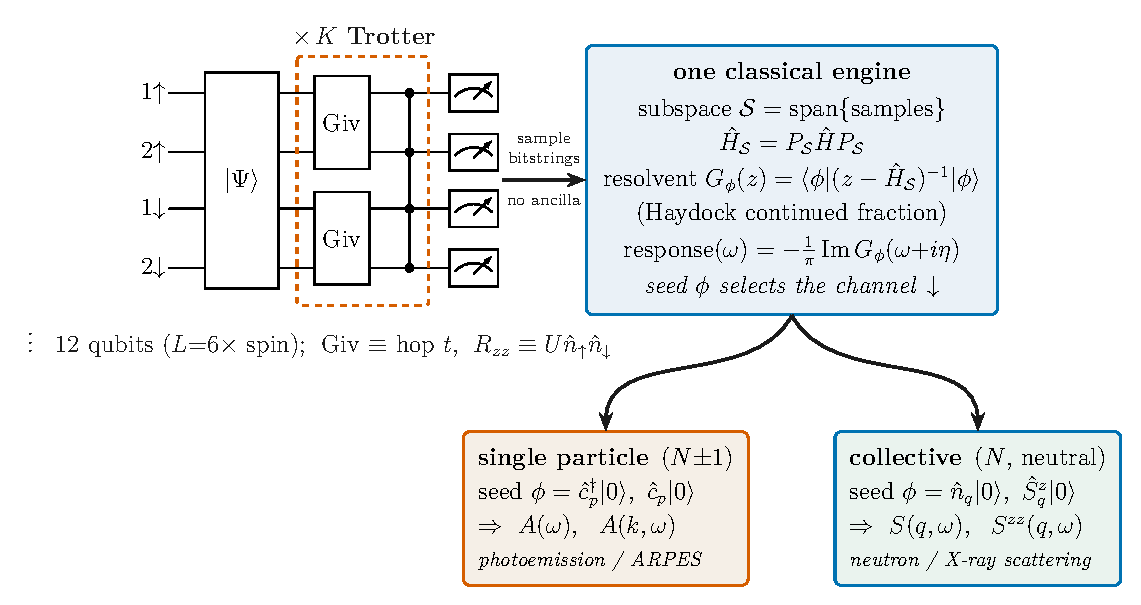
\includegraphics[width=\linewidth]{figs/fig_circuit.pdf}
\caption{\textbf{One sampling primitive, four dynamical responses.} A shallow, ancilla-free
circuit---state preparation and a Trotter layer repeated $K$ times (Givens rotations for the hopping
$t$, native $R_{zz}$ for the on-site $U\hat n_\uparrow\hat n_\downarrow$)---is measured in the
computational basis; no Hadamard test or controlled unitary is run on the device. The sampled
bitstrings define a sector-specific subspace $\mathcal S$ and feed a single classical engine---a Haydock
continued-fraction resolvent~\cite{haydock1972} $G_\phi(z)=\langle\phi|(z-\hat H_{\mathcal S})^{-1}|\phi\rangle$, whose
single-particle case ($\phi=\hat c^\dagger_p|0\rangle$) is the Green's function of
Eq.~\eqref{eq:green}. The seed $\phi$ then selects the channel: particle addition/removal seeds
$\hat c^{\dagger}_p|0\rangle,\hat c_p|0\rangle$ in the $(N{\pm}1)$ sectors give the single-particle
spectral functions $A(\omega)$ and $A(k,\omega)$ (photoemission/ARPES), while number-conserving density
and spin seeds $\hat n_q|0\rangle,\hat S^z_q|0\rangle$ in the $N$ sector give the dynamical structure
factors $S(q,\omega)$ and $S^{zz}(q,\omega)$ (neutron~\cite{squires2012} and resonant inelastic
X-ray~\cite{ament2011} scattering)---all from \emph{one} sampling
primitive, the seed selecting the sector and hence the subspace. The four channels are realized in Figs.~\ref{fig:method} ($A(\omega)$),
\ref{fig:lattice} ($A(k,\omega)$), \ref{fig:sqw} ($S(q,\omega)$), and \ref{fig:spin}
($S^{zz}(q,\omega)$).}\label{fig:circ}\end{figure*}

% carried verbatim from the v2 tree (results.tex); NOT part of this session's deliverable.
\begin{figure*}[tp]\centering% native \input fragment (fig:method) — fonts = document body (11pt) exactly
\definecolor{inkPrim}{HTML}{1B1B1B}\definecolor{inkMute}{HTML}{6E6E6E}\definecolor{clExact}{HTML}{1F3A5F}
\definecolor{coral}{HTML}{F0653F}\definecolor{gridClr}{HTML}{ECEAE5}\definecolor{thm}{HTML}{2E7D5B}
\begin{tikzpicture}[font=\rmfamily]
\begin{groupplot}[
  group style={group size=2 by 1, horizontal sep=1.9cm},
  width=7.7cm, height=5.9cm, paperaxis,
  label style={font=\small}, tick label style={font=\footnotesize},
  axis line style={inkPrim, line width=0.6pt}, tick style={inkPrim, line width=0.6pt},
  title style={yshift=1pt},
]
% ---- (a) A(w): exact vs bitstring-sampled ----
\nextgroupplot[
  xlabel={frequency \; $\omega/t$}, ylabel={$A(\omega)$},
  title={(a)\quad reconstruction of $A(\omega)$ from $5.2\times10^{4}$ shots},
  xmin=3, xmax=14, ymin=0, ymax=0.50, ymajorgrids, y grid style={gridClr},
  legend style={draw=none, fill=white, fill opacity=0.75, text opacity=1, at={(0.985,0.985)}, anchor=north east}, legend cell align=left,
]
  \addplot[draw=none, fill=clExact, fill opacity=0.16, forget plot] table[x=w,y=Aex]{aw_method.dat} \closedcycle;
  \addplot[clExact, line width=1.3pt] table[x=w,y=Aex]{aw_method.dat}; \addlegendentry{exact}
  \addplot[coral, line width=1.1pt, dash pattern=on 3pt off 2.2pt] table[x=w,y=Asm]{aw_method.dat}; \addlegendentry{bitstring-sampled}
  \node[anchor=north east, align=right, inkPrim] at (rel axis cs:0.985,0.56)
     {rel-$L_1=0.017$\\[-1pt] $\int_W\! A_{\mathcal S}=0.4865$};
% ---- (b) convergence: the measured curve only.  The dashed 'geometric (Thm 1)' series
%      and the rho ~ 1.7 label are REMOVED: Sec. 4.2 withdraws that fit and its
%      attribution to the moment theorem. ----
\nextgroupplot[
  xlabel={Krylov order \; $K$ \; (time-evolution steps)}, ylabel={rel-$L_1$ error},
  title={(b)\quad error versus Krylov order},
  xmin=-0.4, xmax=12.4, ymode=log, ymin=0.013, ymax=2.6, ymajorgrids, y grid style={gridClr},
  ytick={0.02,0.05,0.1,0.2,0.5}, yticklabels={$2\%$,$5\%$,$10\%$,$20\%$,$50\%$},
  legend style={draw=none, fill=white, fill opacity=0.85, text opacity=1, at={(0.985,0.985)}, anchor=north east}, legend cell align=left,
]
  \fill[inkMute, fill opacity=0.06] (axis cs:-0.4,0.013) rectangle (axis cs:4,2.6);
  \node[inkPrim, anchor=center, align=center] at (axis cs:1.75,0.19) {discovery\\ regime};
  \addplot[name path=lo, draw=none, forget plot] coordinates {(0,0.5495) (1,0.5169) (2,0.5125) (3,0.5072) (4,0.3953) (5,0.1346) (6,0.0822) (7,0.0481) (8,0.0297) (9,0.0227) (10,0.0191) (11,0.0172) (12,0.0132)};
  \addplot[name path=hi, draw=none, forget plot] coordinates {(0,0.6261) (1,0.6267) (2,0.5807) (3,0.5948) (4,0.4793) (5,0.1820) (6,0.1081) (7,0.0713) (8,0.0402) (9,0.0307) (10,0.0275) (11,0.0259) (12,0.0239)};
  \addplot[coral, fill opacity=0.16, forget plot] fill between[of=lo and hi];
  \addplot[coral, line width=1.3pt, mark=*, mark size=2.2pt,
           mark options={fill=coral, draw=white, line width=0.4pt}] coordinates {(0,0.5878) (1,0.5718) (2,0.5466) (3,0.5510) (4,0.4373) (5,0.1583) (6,0.0951) (7,0.0597) (8,0.0350) (9,0.0267) (10,0.0233) (11,0.0216) (12,0.0185)}; \addlegendentry{sampled (8 seeds)}
\end{groupplot}
\end{tikzpicture}

\caption{\textbf{The method validated at $L=6$, and its error against Krylov order.} \textbf{(a)}~The
bitstring-sampled single-particle spectral function reproduces the exact $A(\omega)$ (Hubbard $L=6$,
$U/t=8$; broadening $\eta=0.15\,t$) to relative-$L_1$ $0.017$---the exact (filled) and reconstructed
(dashed) curves are indistinguishable. The analytic addition-branch sum rule $\int A^{+}\,d\omega=1-\langle n_p\rangle=0.5$ is an identity of
the ground state and not a check on the reconstruction; integrated over the plotted window the exact
and reconstructed curves give $0.486588$ and $0.486471$, agreeing with each other to
$2.4\times10^{-4}$ relative and both falling $2.7\%$ short of $0.5$ because Lorentzian tails leave the
window (Sec.~\ref{sec:physics}). \textbf{(b)}~Convergence of the relative-$L_1$ error with
the Krylov order $K$ (number of time-evolution steps sampled), seed-averaged over eight independent
runs (band $=$ standard deviation), $\eta=0.15\,t$, so the budget is $T=4000(K{+}1)$ and reaches
$5.2\times10^{4}$ at $K=12$. The error falls by a factor $32$ across the thirteen points, from $0.59$
at $K=0$ to $0.0185$ at $K=12$, with one non-monotone step at $K=3$ inside the discovery phase, while
the mean subspace returned grows from $75$ to $242$ determinants of the $300$-dimensional sector. No
geometric rate is fitted to the window $4\le K\le9$ here (Sec.~\ref{sec:moments:notbuy}): one is
not implied by moment exactness, and inside that window the decay in $K$ is confounded with the growth
of $|\mathcal S|$.}\label{fig:method}\end{figure*}

\begin{figure*}[tp]\centering
% Fig. 5 REBUILT 2026-09-18 -- honest labelling of the sampling limit.
% Panels (a),(b): release/data/sampled_akw_L8.json.  sampled_akw.py:47 ranks by the EXACT Born
%   distribution of the time-evolved state, so this is the T->infinity limit of the declared
%   protocol, NOT a finite-shot experiment.  Labelled as such in the title, legend and caption.
% Panel (c): scratchpad/p2_calc/sampled_honest.json, results[L=8]['shot_sweep'] -- the measured
%   finite-shot sweep, 8 seeds, +-1 s.d. band.  DIFFERENT configuration (eta=0.15t, K=18 slices,
%   local seed c^dag_{0,up}, addition branch only): declared in the caption.  No extrapolation.
% Every coordinate and every printed number is emitted by make_fig5_honest.py from those JSONs.
\definecolor{akExact}{HTML}{1B1B1B}\definecolor{akSamp}{HTML}{D55E00}\definecolor{akInk}{HTML}{1B1B1B}\definecolor{akShot}{HTML}{0072B2}
\begin{tikzpicture}
\begin{axis}[name=pa, width=14.05cm, height=6.3cm, paperaxis,
  title={(a)~exact $A(k,\omega)$ versus the reconstruction on the top-$85\%$ Born subspace},
  title style={at={(0,1)},anchor=south west,font=\normalsize\bfseries,yshift=15pt},
  label style={font=\normalsize}, tick label style={font=\footnotesize},
  xlabel={$\omega-E_0\ (t)$}, ylabel={$A(k,\omega)$ (offset by $k$)},
  xmin=-9,xmax=9, ymin=-0.3,ymax=2.85, ytick=\empty, xtick={-8,-6,-4,-2,0,2,4,6,8},
  legend style={font=\footnotesize,at={(1,1.005)},anchor=south east,legend columns=2,draw=none,fill=none,/tikz/every even column/.append style={column sep=10pt}},legend cell align=left]
\addplot[akExact,line width=1.2pt,fill=akExact,fill opacity=0.06] coordinates {(-9.000,0.0007) (-8.970,0.0007) (-8.940,0.0007) (-8.910,0.0007) (-8.880,0.0007) (-8.850,0.0007) (-8.820,0.0007) (-8.790,0.0007) (-8.760,0.0007) (-8.730,0.0007) (-8.699,0.0007) (-8.669,0.0007) (-8.639,0.0007) (-8.609,0.0007) (-8.579,0.0007) (-8.549,0.0008) (-8.519,0.0008) (-8.489,0.0008) (-8.459,0.0008) (-8.429,0.0008) (-8.399,0.0008) (-8.369,0.0008) (-8.339,0.0008) (-8.309,0.0008) (-8.279,0.0008) (-8.249,0.0008) (-8.219,0.0008) (-8.189,0.0008) (-8.159,0.0008) (-8.129,0.0008) (-8.098,0.0008) (-8.068,0.0008) (-8.038,0.0008) (-8.008,0.0008) (-7.978,0.0008) (-7.948,0.0008) (-7.918,0.0008) (-7.888,0.0008) (-7.858,0.0009) (-7.828,0.0009) (-7.798,0.0009) (-7.768,0.0009) (-7.738,0.0009) (-7.708,0.0009) (-7.678,0.0009) (-7.648,0.0009) (-7.618,0.0009) (-7.588,0.0009) (-7.558,0.0009) (-7.528,0.0009) (-7.497,0.0009) (-7.467,0.0009) (-7.437,0.0009) (-7.407,0.0009) (-7.377,0.0009) (-7.347,0.0009) (-7.317,0.0010) (-7.287,0.0010) (-7.257,0.0010) (-7.227,0.0010) (-7.197,0.0010) (-7.167,0.0010) (-7.137,0.0010) (-7.107,0.0010) (-7.077,0.0010) (-7.047,0.0010) (-7.017,0.0011) (-6.987,0.0011) (-6.957,0.0011) (-6.927,0.0011) (-6.896,0.0011) (-6.866,0.0011) (-6.836,0.0011) (-6.806,0.0011) (-6.776,0.0011) (-6.746,0.0011) (-6.716,0.0011) (-6.686,0.0011) (-6.656,0.0011) (-6.626,0.0011) (-6.596,0.0011) (-6.566,0.0011) (-6.536,0.0012) (-6.506,0.0012) (-6.476,0.0012) (-6.446,0.0012) (-6.416,0.0012) (-6.386,0.0012) (-6.356,0.0012) (-6.326,0.0012) (-6.295,0.0012) (-6.265,0.0013) (-6.235,0.0013) (-6.205,0.0013) (-6.175,0.0013) (-6.145,0.0013) (-6.115,0.0013) (-6.085,0.0013) (-6.055,0.0014) (-6.025,0.0014) (-5.995,0.0014) (-5.965,0.0014) (-5.935,0.0014) (-5.905,0.0014) (-5.875,0.0015) (-5.845,0.0015) (-5.815,0.0015) (-5.785,0.0015) (-5.755,0.0015) (-5.725,0.0016) (-5.694,0.0016) (-5.664,0.0016) (-5.634,0.0017) (-5.604,0.0017) (-5.574,0.0017) (-5.544,0.0017) (-5.514,0.0017) (-5.484,0.0017) (-5.454,0.0018) (-5.424,0.0018) (-5.394,0.0018) (-5.364,0.0018) (-5.334,0.0018) (-5.304,0.0018) (-5.274,0.0018) (-5.244,0.0018) (-5.214,0.0018) (-5.184,0.0019) (-5.154,0.0019) (-5.124,0.0019) (-5.093,0.0019) (-5.063,0.0019) (-5.033,0.0020) (-5.003,0.0020) (-4.973,0.0020) (-4.943,0.0020) (-4.913,0.0021) (-4.883,0.0021) (-4.853,0.0021) (-4.823,0.0021) (-4.793,0.0022) (-4.763,0.0022) (-4.733,0.0022) (-4.703,0.0023) (-4.673,0.0023) (-4.643,0.0023) (-4.613,0.0023) (-4.583,0.0024) (-4.553,0.0024) (-4.523,0.0024) (-4.492,0.0025) (-4.462,0.0025) (-4.432,0.0026) (-4.402,0.0026) (-4.372,0.0026) (-4.342,0.0027) (-4.312,0.0027) (-4.282,0.0027) (-4.252,0.0028) (-4.222,0.0028) (-4.192,0.0029) (-4.162,0.0029) (-4.132,0.0030) (-4.102,0.0030) (-4.072,0.0031) (-4.042,0.0031) (-4.012,0.0032) (-3.982,0.0032) (-3.952,0.0033) (-3.922,0.0033) (-3.891,0.0034) (-3.861,0.0034) (-3.831,0.0035) (-3.801,0.0036) (-3.771,0.0036) (-3.741,0.0037) (-3.711,0.0037) (-3.681,0.0038) (-3.651,0.0039) (-3.621,0.0040) (-3.591,0.0040) (-3.561,0.0041) (-3.531,0.0042) (-3.501,0.0043) (-3.471,0.0044) (-3.441,0.0045) (-3.411,0.0045) (-3.381,0.0046) (-3.351,0.0047) (-3.321,0.0048) (-3.290,0.0049) (-3.260,0.0050) (-3.230,0.0051) (-3.200,0.0052) (-3.170,0.0054) (-3.140,0.0055) (-3.110,0.0056) (-3.080,0.0057) (-3.050,0.0059) (-3.020,0.0060) (-2.990,0.0062) (-2.960,0.0064) (-2.930,0.0066) (-2.900,0.0068) (-2.870,0.0070) (-2.840,0.0072) (-2.810,0.0075) (-2.780,0.0077) (-2.750,0.0079) (-2.720,0.0081) (-2.689,0.0083) (-2.659,0.0084) (-2.629,0.0086) (-2.599,0.0087) (-2.569,0.0089) (-2.539,0.0091) (-2.509,0.0093) (-2.479,0.0095) (-2.449,0.0097) (-2.419,0.0100) (-2.389,0.0103) (-2.359,0.0106) (-2.329,0.0109) (-2.299,0.0112) (-2.269,0.0116) (-2.239,0.0119) (-2.209,0.0123) (-2.179,0.0128) (-2.149,0.0132) (-2.119,0.0137) (-2.088,0.0142) (-2.058,0.0147) (-2.028,0.0153) (-1.998,0.0159) (-1.968,0.0166) (-1.938,0.0173) (-1.908,0.0180) (-1.878,0.0188) (-1.848,0.0196) (-1.818,0.0205) (-1.788,0.0215) (-1.758,0.0226) (-1.728,0.0237) (-1.698,0.0250) (-1.668,0.0263) (-1.638,0.0278) (-1.608,0.0294) (-1.578,0.0311) (-1.548,0.0329) (-1.518,0.0349) (-1.487,0.0371) (-1.457,0.0395) (-1.427,0.0421) (-1.397,0.0451) (-1.367,0.0483) (-1.337,0.0520) (-1.307,0.0562) (-1.277,0.0609) (-1.247,0.0663) (-1.217,0.0724) (-1.187,0.0794) (-1.157,0.0874) (-1.127,0.0968) (-1.097,0.1078) (-1.067,0.1207) (-1.037,0.1359) (-1.007,0.1541) (-0.977,0.1760) (-0.947,0.2024) (-0.917,0.2344) (-0.886,0.2733) (-0.856,0.3204) (-0.826,0.3771) (-0.796,0.4437) (-0.766,0.5187) (-0.736,0.5969) (-0.706,0.6682) (-0.676,0.7182) (-0.646,0.7339) (-0.616,0.7105) (-0.586,0.6553) (-0.556,0.5824) (-0.526,0.5054) (-0.496,0.4333) (-0.466,0.3702) (-0.436,0.3171) (-0.406,0.2734) (-0.376,0.2376) (-0.346,0.2085) (-0.316,0.1849) (-0.285,0.1656) (-0.255,0.1500) (-0.225,0.1373) (-0.195,0.1269) (-0.165,0.1187) (-0.135,0.1121) (-0.105,0.1070) (-0.075,0.1032) (-0.045,0.1007) (-0.015,0.0992) (0.015,0.0988) (0.045,0.0995) (0.075,0.1012) (0.105,0.1041) (0.135,0.1082) (0.165,0.1137) (0.195,0.1208) (0.225,0.1297) (0.255,0.1409) (0.285,0.1546) (0.316,0.1716) (0.346,0.1925) (0.376,0.2183) (0.406,0.2501) (0.436,0.2890) (0.466,0.3365) (0.496,0.3933) (0.526,0.4590) (0.556,0.5306) (0.586,0.6010) (0.616,0.6583) (0.646,0.6887) (0.676,0.6832) (0.706,0.6433) (0.736,0.5799) (0.766,0.5069) (0.796,0.4351) (0.826,0.3703) (0.856,0.3147) (0.886,0.2682) (0.917,0.2297) (0.947,0.1981) (0.977,0.1721) (1.007,0.1506) (1.037,0.1327) (1.067,0.1176) (1.097,0.1050) (1.127,0.0942) (1.157,0.0850) (1.187,0.0771) (1.217,0.0703) (1.247,0.0643) (1.277,0.0591) (1.307,0.0545) (1.337,0.0504) (1.367,0.0468) (1.397,0.0435) (1.427,0.0406) (1.457,0.0380) (1.487,0.0357) (1.518,0.0335) (1.548,0.0316) (1.578,0.0298) (1.608,0.0282) (1.638,0.0267) (1.668,0.0253) (1.698,0.0241) (1.728,0.0229) (1.758,0.0218) (1.788,0.0208) (1.818,0.0199) (1.848,0.0191) (1.878,0.0182) (1.908,0.0175) (1.938,0.0168) (1.968,0.0161) (1.998,0.0155) (2.028,0.0149) (2.058,0.0144) (2.088,0.0139) (2.119,0.0134) (2.149,0.0129) (2.179,0.0125) (2.209,0.0121) (2.239,0.0117) (2.269,0.0113) (2.299,0.0109) (2.329,0.0106) (2.359,0.0103) (2.389,0.0100) (2.419,0.0097) (2.449,0.0094) (2.479,0.0092) (2.509,0.0089) (2.539,0.0087) (2.569,0.0084) (2.599,0.0082) (2.629,0.0080) (2.659,0.0078) (2.689,0.0076) (2.720,0.0074) (2.750,0.0072) (2.780,0.0071) (2.810,0.0069) (2.840,0.0068) (2.870,0.0066) (2.900,0.0065) (2.930,0.0063) (2.960,0.0062) (2.990,0.0060) (3.020,0.0059) (3.050,0.0058) (3.080,0.0057) (3.110,0.0056) (3.140,0.0054) (3.170,0.0053) (3.200,0.0052) (3.230,0.0051) (3.260,0.0050) (3.290,0.0050) (3.321,0.0049) (3.351,0.0048) (3.381,0.0047) (3.411,0.0046) (3.441,0.0045) (3.471,0.0045) (3.501,0.0044) (3.531,0.0043) (3.561,0.0042) (3.591,0.0042) (3.621,0.0041) (3.651,0.0040) (3.681,0.0040) (3.711,0.0039) (3.741,0.0039) (3.771,0.0038) (3.801,0.0037) (3.831,0.0037) (3.861,0.0036) (3.891,0.0036) (3.922,0.0035) (3.952,0.0035) (3.982,0.0034) (4.012,0.0034) (4.042,0.0034) (4.072,0.0033) (4.102,0.0033) (4.132,0.0032) (4.162,0.0032) (4.192,0.0032) (4.222,0.0031) (4.252,0.0031) (4.282,0.0030) (4.312,0.0030) (4.342,0.0030) (4.372,0.0029) (4.402,0.0029) (4.432,0.0029) (4.462,0.0029) (4.492,0.0028) (4.523,0.0028) (4.553,0.0028) (4.583,0.0027) (4.613,0.0027) (4.643,0.0027) (4.673,0.0027) (4.703,0.0027) (4.733,0.0026) (4.763,0.0026) (4.793,0.0026) (4.823,0.0026) (4.853,0.0025) (4.883,0.0025) (4.913,0.0025) (4.943,0.0025) (4.973,0.0025) (5.003,0.0025) (5.033,0.0024) (5.063,0.0024) (5.093,0.0024) (5.124,0.0024) (5.154,0.0024) (5.184,0.0024) (5.214,0.0024) (5.244,0.0023) (5.274,0.0023) (5.304,0.0023) (5.334,0.0023) (5.364,0.0023) (5.394,0.0023) (5.424,0.0023) (5.454,0.0023) (5.484,0.0023) (5.514,0.0023) (5.544,0.0023) (5.574,0.0023) (5.604,0.0022) (5.634,0.0022) (5.664,0.0022) (5.694,0.0022) (5.725,0.0022) (5.755,0.0022) (5.785,0.0022) (5.815,0.0022) (5.845,0.0022) (5.875,0.0022) (5.905,0.0022) (5.935,0.0022) (5.965,0.0022) (5.995,0.0022) (6.025,0.0022) (6.055,0.0022) (6.085,0.0022) (6.115,0.0022) (6.145,0.0023) (6.175,0.0023) (6.205,0.0023) (6.235,0.0023) (6.265,0.0023) (6.295,0.0023) (6.326,0.0023) (6.356,0.0023) (6.386,0.0023) (6.416,0.0023) (6.446,0.0024) (6.476,0.0024) (6.506,0.0024) (6.536,0.0024) (6.566,0.0024) (6.596,0.0025) (6.626,0.0025) (6.656,0.0025) (6.686,0.0025) (6.716,0.0026) (6.746,0.0026) (6.776,0.0026) (6.806,0.0026) (6.836,0.0027) (6.866,0.0027) (6.896,0.0028) (6.927,0.0028) (6.957,0.0029) (6.987,0.0029) (7.017,0.0030) (7.047,0.0030) (7.077,0.0031) (7.107,0.0032) (7.137,0.0033) (7.167,0.0034) (7.197,0.0035) (7.227,0.0036) (7.257,0.0038) (7.287,0.0039) (7.317,0.0041) (7.347,0.0043) (7.377,0.0046) (7.407,0.0048) (7.437,0.0050) (7.467,0.0052) (7.497,0.0052) (7.528,0.0052) (7.558,0.0051) (7.588,0.0050) (7.618,0.0049) (7.648,0.0049) (7.678,0.0049) (7.708,0.0049) (7.738,0.0049) (7.768,0.0049) (7.798,0.0050) (7.828,0.0051) (7.858,0.0052) (7.888,0.0053) (7.918,0.0055) (7.948,0.0056) (7.978,0.0058) (8.008,0.0060) (8.038,0.0062) (8.068,0.0064) (8.098,0.0067) (8.129,0.0070) (8.159,0.0073) (8.189,0.0076) (8.219,0.0080) (8.249,0.0084) (8.279,0.0088) (8.309,0.0092) (8.339,0.0097) (8.369,0.0101) (8.399,0.0105) (8.429,0.0110) (8.459,0.0115) (8.489,0.0120) (8.519,0.0126) (8.549,0.0133) (8.579,0.0141) (8.609,0.0150) (8.639,0.0160) (8.669,0.0171) (8.699,0.0183) (8.730,0.0197) (8.760,0.0213) (8.790,0.0231) (8.820,0.0251) (8.850,0.0274) (8.880,0.0301) (8.910,0.0331) (8.940,0.0367) (8.970,0.0409) (9.000,0.0457)} \closedcycle;
\addplot[akSamp,line width=1.1pt,dash pattern=on 4pt off 2.5pt] coordinates {(-9.000,0.0007) (-8.970,0.0007) (-8.940,0.0007) (-8.910,0.0007) (-8.880,0.0007) (-8.850,0.0007) (-8.820,0.0007) (-8.790,0.0007) (-8.760,0.0007) (-8.730,0.0007) (-8.699,0.0007) (-8.669,0.0007) (-8.639,0.0007) (-8.609,0.0007) (-8.579,0.0008) (-8.549,0.0008) (-8.519,0.0008) (-8.489,0.0008) (-8.459,0.0008) (-8.429,0.0008) (-8.399,0.0008) (-8.369,0.0008) (-8.339,0.0008) (-8.309,0.0008) (-8.279,0.0008) (-8.249,0.0008) (-8.219,0.0008) (-8.189,0.0008) (-8.159,0.0008) (-8.129,0.0008) (-8.098,0.0008) (-8.068,0.0008) (-8.038,0.0008) (-8.008,0.0008) (-7.978,0.0008) (-7.948,0.0008) (-7.918,0.0008) (-7.888,0.0008) (-7.858,0.0008) (-7.828,0.0008) (-7.798,0.0008) (-7.768,0.0009) (-7.738,0.0009) (-7.708,0.0009) (-7.678,0.0009) (-7.648,0.0009) (-7.618,0.0009) (-7.588,0.0009) (-7.558,0.0009) (-7.528,0.0009) (-7.497,0.0009) (-7.467,0.0009) (-7.437,0.0009) (-7.407,0.0009) (-7.377,0.0009) (-7.347,0.0010) (-7.317,0.0010) (-7.287,0.0010) (-7.257,0.0010) (-7.227,0.0010) (-7.197,0.0010) (-7.167,0.0010) (-7.137,0.0010) (-7.107,0.0010) (-7.077,0.0010) (-7.047,0.0010) (-7.017,0.0010) (-6.987,0.0011) (-6.957,0.0011) (-6.927,0.0011) (-6.896,0.0011) (-6.866,0.0011) (-6.836,0.0011) (-6.806,0.0011) (-6.776,0.0011) (-6.746,0.0011) (-6.716,0.0011) (-6.686,0.0011) (-6.656,0.0011) (-6.626,0.0011) (-6.596,0.0011) (-6.566,0.0011) (-6.536,0.0012) (-6.506,0.0012) (-6.476,0.0012) (-6.446,0.0012) (-6.416,0.0012) (-6.386,0.0012) (-6.356,0.0012) (-6.326,0.0012) (-6.295,0.0013) (-6.265,0.0013) (-6.235,0.0013) (-6.205,0.0013) (-6.175,0.0013) (-6.145,0.0013) (-6.115,0.0013) (-6.085,0.0013) (-6.055,0.0014) (-6.025,0.0014) (-5.995,0.0014) (-5.965,0.0014) (-5.935,0.0014) (-5.905,0.0015) (-5.875,0.0015) (-5.845,0.0015) (-5.815,0.0015) (-5.785,0.0015) (-5.755,0.0016) (-5.725,0.0016) (-5.694,0.0016) (-5.664,0.0017) (-5.634,0.0017) (-5.604,0.0017) (-5.574,0.0017) (-5.544,0.0017) (-5.514,0.0017) (-5.484,0.0017) (-5.454,0.0017) (-5.424,0.0017) (-5.394,0.0017) (-5.364,0.0018) (-5.334,0.0018) (-5.304,0.0018) (-5.274,0.0018) (-5.244,0.0018) (-5.214,0.0018) (-5.184,0.0019) (-5.154,0.0019) (-5.124,0.0019) (-5.093,0.0019) (-5.063,0.0019) (-5.033,0.0020) (-5.003,0.0020) (-4.973,0.0020) (-4.943,0.0020) (-4.913,0.0021) (-4.883,0.0021) (-4.853,0.0021) (-4.823,0.0021) (-4.793,0.0022) (-4.763,0.0022) (-4.733,0.0022) (-4.703,0.0023) (-4.673,0.0023) (-4.643,0.0023) (-4.613,0.0023) (-4.583,0.0024) (-4.553,0.0024) (-4.523,0.0024) (-4.492,0.0025) (-4.462,0.0025) (-4.432,0.0026) (-4.402,0.0026) (-4.372,0.0026) (-4.342,0.0027) (-4.312,0.0027) (-4.282,0.0027) (-4.252,0.0028) (-4.222,0.0028) (-4.192,0.0029) (-4.162,0.0029) (-4.132,0.0030) (-4.102,0.0030) (-4.072,0.0031) (-4.042,0.0031) (-4.012,0.0032) (-3.982,0.0032) (-3.952,0.0033) (-3.922,0.0033) (-3.891,0.0034) (-3.861,0.0034) (-3.831,0.0035) (-3.801,0.0036) (-3.771,0.0036) (-3.741,0.0037) (-3.711,0.0037) (-3.681,0.0038) (-3.651,0.0039) (-3.621,0.0040) (-3.591,0.0040) (-3.561,0.0041) (-3.531,0.0042) (-3.501,0.0043) (-3.471,0.0044) (-3.441,0.0045) (-3.411,0.0046) (-3.381,0.0046) (-3.351,0.0047) (-3.321,0.0048) (-3.290,0.0049) (-3.260,0.0050) (-3.230,0.0051) (-3.200,0.0052) (-3.170,0.0054) (-3.140,0.0055) (-3.110,0.0056) (-3.080,0.0057) (-3.050,0.0059) (-3.020,0.0060) (-2.990,0.0062) (-2.960,0.0064) (-2.930,0.0066) (-2.900,0.0068) (-2.870,0.0070) (-2.840,0.0072) (-2.810,0.0075) (-2.780,0.0077) (-2.750,0.0079) (-2.720,0.0081) (-2.689,0.0083) (-2.659,0.0084) (-2.629,0.0086) (-2.599,0.0087) (-2.569,0.0089) (-2.539,0.0091) (-2.509,0.0093) (-2.479,0.0095) (-2.449,0.0097) (-2.419,0.0100) (-2.389,0.0103) (-2.359,0.0106) (-2.329,0.0109) (-2.299,0.0112) (-2.269,0.0116) (-2.239,0.0119) (-2.209,0.0123) (-2.179,0.0128) (-2.149,0.0132) (-2.119,0.0137) (-2.088,0.0142) (-2.058,0.0147) (-2.028,0.0153) (-1.998,0.0159) (-1.968,0.0166) (-1.938,0.0173) (-1.908,0.0180) (-1.878,0.0188) (-1.848,0.0196) (-1.818,0.0206) (-1.788,0.0215) (-1.758,0.0226) (-1.728,0.0237) (-1.698,0.0250) (-1.668,0.0263) (-1.638,0.0278) (-1.608,0.0294) (-1.578,0.0311) (-1.548,0.0329) (-1.518,0.0349) (-1.487,0.0371) (-1.457,0.0395) (-1.427,0.0422) (-1.397,0.0451) (-1.367,0.0484) (-1.337,0.0521) (-1.307,0.0563) (-1.277,0.0610) (-1.247,0.0663) (-1.217,0.0724) (-1.187,0.0795) (-1.157,0.0875) (-1.127,0.0969) (-1.097,0.1079) (-1.067,0.1208) (-1.037,0.1361) (-1.007,0.1544) (-0.977,0.1763) (-0.947,0.2027) (-0.917,0.2348) (-0.886,0.2738) (-0.856,0.3210) (-0.826,0.3778) (-0.796,0.4445) (-0.766,0.5196) (-0.736,0.5978) (-0.706,0.6689) (-0.676,0.7187) (-0.646,0.7339) (-0.616,0.7102) (-0.586,0.6547) (-0.556,0.5816) (-0.526,0.5046) (-0.496,0.4326) (-0.466,0.3696) (-0.436,0.3167) (-0.406,0.2730) (-0.376,0.2373) (-0.346,0.2083) (-0.316,0.1847) (-0.285,0.1655) (-0.255,0.1498) (-0.225,0.1371) (-0.195,0.1268) (-0.165,0.1186) (-0.135,0.1120) (-0.105,0.1069) (-0.075,0.1032) (-0.045,0.1006) (-0.015,0.0992) (0.015,0.0988) (0.045,0.0994) (0.075,0.1012) (0.105,0.1041) (0.135,0.1082) (0.165,0.1137) (0.195,0.1208) (0.225,0.1298) (0.255,0.1409) (0.285,0.1547) (0.316,0.1717) (0.346,0.1926) (0.376,0.2184) (0.406,0.2502) (0.436,0.2892) (0.466,0.3366) (0.496,0.3934) (0.526,0.4592) (0.556,0.5308) (0.586,0.6012) (0.616,0.6584) (0.646,0.6886) (0.676,0.6829) (0.706,0.6429) (0.736,0.5795) (0.766,0.5065) (0.796,0.4347) (0.826,0.3699) (0.856,0.3144) (0.886,0.2679) (0.917,0.2295) (0.947,0.1980) (0.977,0.1720) (1.007,0.1505) (1.037,0.1326) (1.067,0.1176) (1.097,0.1049) (1.127,0.0942) (1.157,0.0850) (1.187,0.0771) (1.217,0.0702) (1.247,0.0643) (1.277,0.0590) (1.307,0.0544) (1.337,0.0504) (1.367,0.0467) (1.397,0.0435) (1.427,0.0406) (1.457,0.0380) (1.487,0.0357) (1.518,0.0335) (1.548,0.0316) (1.578,0.0298) (1.608,0.0282) (1.638,0.0267) (1.668,0.0253) (1.698,0.0241) (1.728,0.0229) (1.758,0.0218) (1.788,0.0208) (1.818,0.0199) (1.848,0.0190) (1.878,0.0182) (1.908,0.0175) (1.938,0.0168) (1.968,0.0161) (1.998,0.0155) (2.028,0.0149) (2.058,0.0144) (2.088,0.0139) (2.119,0.0134) (2.149,0.0129) (2.179,0.0125) (2.209,0.0121) (2.239,0.0117) (2.269,0.0113) (2.299,0.0109) (2.329,0.0106) (2.359,0.0103) (2.389,0.0100) (2.419,0.0097) (2.449,0.0094) (2.479,0.0092) (2.509,0.0089) (2.539,0.0087) (2.569,0.0084) (2.599,0.0082) (2.629,0.0080) (2.659,0.0078) (2.689,0.0076) (2.720,0.0074) (2.750,0.0072) (2.780,0.0071) (2.810,0.0069) (2.840,0.0067) (2.870,0.0066) (2.900,0.0064) (2.930,0.0063) (2.960,0.0062) (2.990,0.0060) (3.020,0.0059) (3.050,0.0058) (3.080,0.0057) (3.110,0.0056) (3.140,0.0054) (3.170,0.0053) (3.200,0.0052) (3.230,0.0051) (3.260,0.0050) (3.290,0.0050) (3.321,0.0049) (3.351,0.0048) (3.381,0.0047) (3.411,0.0046) (3.441,0.0045) (3.471,0.0045) (3.501,0.0044) (3.531,0.0043) (3.561,0.0042) (3.591,0.0042) (3.621,0.0041) (3.651,0.0040) (3.681,0.0040) (3.711,0.0039) (3.741,0.0039) (3.771,0.0038) (3.801,0.0037) (3.831,0.0037) (3.861,0.0036) (3.891,0.0036) (3.922,0.0035) (3.952,0.0035) (3.982,0.0034) (4.012,0.0034) (4.042,0.0034) (4.072,0.0033) (4.102,0.0033) (4.132,0.0032) (4.162,0.0032) (4.192,0.0032) (4.222,0.0031) (4.252,0.0031) (4.282,0.0030) (4.312,0.0030) (4.342,0.0030) (4.372,0.0029) (4.402,0.0029) (4.432,0.0029) (4.462,0.0029) (4.492,0.0028) (4.523,0.0028) (4.553,0.0028) (4.583,0.0027) (4.613,0.0027) (4.643,0.0027) (4.673,0.0027) (4.703,0.0027) (4.733,0.0026) (4.763,0.0026) (4.793,0.0026) (4.823,0.0026) (4.853,0.0025) (4.883,0.0025) (4.913,0.0025) (4.943,0.0025) (4.973,0.0025) (5.003,0.0025) (5.033,0.0024) (5.063,0.0024) (5.093,0.0024) (5.124,0.0024) (5.154,0.0024) (5.184,0.0024) (5.214,0.0024) (5.244,0.0023) (5.274,0.0023) (5.304,0.0023) (5.334,0.0023) (5.364,0.0023) (5.394,0.0023) (5.424,0.0023) (5.454,0.0023) (5.484,0.0023) (5.514,0.0023) (5.544,0.0023) (5.574,0.0023) (5.604,0.0022) (5.634,0.0022) (5.664,0.0022) (5.694,0.0022) (5.725,0.0022) (5.755,0.0022) (5.785,0.0022) (5.815,0.0022) (5.845,0.0022) (5.875,0.0022) (5.905,0.0022) (5.935,0.0022) (5.965,0.0022) (5.995,0.0022) (6.025,0.0022) (6.055,0.0022) (6.085,0.0022) (6.115,0.0022) (6.145,0.0023) (6.175,0.0023) (6.205,0.0023) (6.235,0.0023) (6.265,0.0023) (6.295,0.0023) (6.326,0.0023) (6.356,0.0023) (6.386,0.0023) (6.416,0.0023) (6.446,0.0024) (6.476,0.0024) (6.506,0.0024) (6.536,0.0024) (6.566,0.0024) (6.596,0.0025) (6.626,0.0025) (6.656,0.0025) (6.686,0.0025) (6.716,0.0026) (6.746,0.0026) (6.776,0.0026) (6.806,0.0026) (6.836,0.0027) (6.866,0.0027) (6.896,0.0028) (6.927,0.0028) (6.957,0.0029) (6.987,0.0029) (7.017,0.0030) (7.047,0.0030) (7.077,0.0031) (7.107,0.0032) (7.137,0.0033) (7.167,0.0034) (7.197,0.0035) (7.227,0.0036) (7.257,0.0037) (7.287,0.0039) (7.317,0.0041) (7.347,0.0043) (7.377,0.0046) (7.407,0.0048) (7.437,0.0050) (7.467,0.0052) (7.497,0.0052) (7.528,0.0052) (7.558,0.0051) (7.588,0.0050) (7.618,0.0049) (7.648,0.0049) (7.678,0.0049) (7.708,0.0049) (7.738,0.0049) (7.768,0.0049) (7.798,0.0050) (7.828,0.0051) (7.858,0.0052) (7.888,0.0053) (7.918,0.0055) (7.948,0.0056) (7.978,0.0058) (8.008,0.0060) (8.038,0.0062) (8.068,0.0064) (8.098,0.0067) (8.129,0.0070) (8.159,0.0073) (8.189,0.0076) (8.219,0.0080) (8.249,0.0084) (8.279,0.0088) (8.309,0.0092) (8.339,0.0097) (8.369,0.0101) (8.399,0.0105) (8.429,0.0110) (8.459,0.0114) (8.489,0.0120) (8.519,0.0126) (8.549,0.0133) (8.579,0.0141) (8.609,0.0150) (8.639,0.0160) (8.669,0.0171) (8.699,0.0183) (8.730,0.0197) (8.760,0.0213) (8.790,0.0231) (8.820,0.0251) (8.850,0.0274) (8.880,0.0300) (8.910,0.0331) (8.940,0.0366) (8.970,0.0408) (9.000,0.0456)};
\addlegendentry{exact (Haydock)}
\addlegendentry{top-$85\%$ Born subspace, infinite-shot limit $T\rightarrow\infty$}
\node[akInk,font=\footnotesize,anchor=west] at (axis cs:-8.75,0.1550) {$k{=}0$};
\addplot[akExact,line width=1.2pt,fill=akExact,fill opacity=0.06] coordinates {(-9.000,0.7711) (-8.970,0.7711) (-8.940,0.7711) (-8.910,0.7711) (-8.880,0.7711) (-8.850,0.7711) (-8.820,0.7711) (-8.790,0.7711) (-8.760,0.7711) (-8.730,0.7711) (-8.699,0.7711) (-8.669,0.7711) (-8.639,0.7711) (-8.609,0.7711) (-8.579,0.7711) (-8.549,0.7712) (-8.519,0.7712) (-8.489,0.7712) (-8.459,0.7712) (-8.429,0.7712) (-8.399,0.7712) (-8.369,0.7712) (-8.339,0.7712) (-8.309,0.7712) (-8.279,0.7712) (-8.249,0.7712) (-8.219,0.7712) (-8.189,0.7712) (-8.159,0.7712) (-8.129,0.7712) (-8.098,0.7712) (-8.068,0.7712) (-8.038,0.7712) (-8.008,0.7712) (-7.978,0.7712) (-7.948,0.7712) (-7.918,0.7712) (-7.888,0.7712) (-7.858,0.7713) (-7.828,0.7713) (-7.798,0.7713) (-7.768,0.7713) (-7.738,0.7713) (-7.708,0.7713) (-7.678,0.7713) (-7.648,0.7713) (-7.618,0.7713) (-7.588,0.7713) (-7.558,0.7713) (-7.528,0.7713) (-7.497,0.7713) (-7.467,0.7713) (-7.437,0.7713) (-7.407,0.7713) (-7.377,0.7713) (-7.347,0.7713) (-7.317,0.7713) (-7.287,0.7713) (-7.257,0.7714) (-7.227,0.7714) (-7.197,0.7714) (-7.167,0.7714) (-7.137,0.7714) (-7.107,0.7714) (-7.077,0.7714) (-7.047,0.7714) (-7.017,0.7715) (-6.987,0.7715) (-6.957,0.7715) (-6.927,0.7715) (-6.896,0.7715) (-6.866,0.7715) (-6.836,0.7715) (-6.806,0.7715) (-6.776,0.7715) (-6.746,0.7715) (-6.716,0.7715) (-6.686,0.7715) (-6.656,0.7715) (-6.626,0.7715) (-6.596,0.7715) (-6.566,0.7715) (-6.536,0.7715) (-6.506,0.7715) (-6.476,0.7715) (-6.446,0.7715) (-6.416,0.7715) (-6.386,0.7715) (-6.356,0.7716) (-6.326,0.7716) (-6.295,0.7716) (-6.265,0.7716) (-6.235,0.7716) (-6.205,0.7716) (-6.175,0.7716) (-6.145,0.7716) (-6.115,0.7717) (-6.085,0.7717) (-6.055,0.7717) (-6.025,0.7717) (-5.995,0.7717) (-5.965,0.7717) (-5.935,0.7717) (-5.905,0.7717) (-5.875,0.7717) (-5.845,0.7718) (-5.815,0.7718) (-5.785,0.7718) (-5.755,0.7718) (-5.725,0.7718) (-5.694,0.7718) (-5.664,0.7718) (-5.634,0.7719) (-5.604,0.7719) (-5.574,0.7719) (-5.544,0.7719) (-5.514,0.7719) (-5.484,0.7719) (-5.454,0.7720) (-5.424,0.7720) (-5.394,0.7720) (-5.364,0.7720) (-5.334,0.7721) (-5.304,0.7721) (-5.274,0.7721) (-5.244,0.7721) (-5.214,0.7721) (-5.184,0.7722) (-5.154,0.7722) (-5.124,0.7722) (-5.093,0.7723) (-5.063,0.7723) (-5.033,0.7723) (-5.003,0.7723) (-4.973,0.7724) (-4.943,0.7724) (-4.913,0.7724) (-4.883,0.7724) (-4.853,0.7725) (-4.823,0.7725) (-4.793,0.7725) (-4.763,0.7726) (-4.733,0.7726) (-4.703,0.7726) (-4.673,0.7727) (-4.643,0.7727) (-4.613,0.7728) (-4.583,0.7728) (-4.553,0.7729) (-4.523,0.7729) (-4.492,0.7730) (-4.462,0.7730) (-4.432,0.7731) (-4.402,0.7731) (-4.372,0.7732) (-4.342,0.7732) (-4.312,0.7733) (-4.282,0.7734) (-4.252,0.7734) (-4.222,0.7735) (-4.192,0.7736) (-4.162,0.7737) (-4.132,0.7737) (-4.102,0.7738) (-4.072,0.7739) (-4.042,0.7740) (-4.012,0.7741) (-3.982,0.7742) (-3.952,0.7743) (-3.922,0.7744) (-3.891,0.7746) (-3.861,0.7747) (-3.831,0.7748) (-3.801,0.7750) (-3.771,0.7751) (-3.741,0.7753) (-3.711,0.7755) (-3.681,0.7757) (-3.651,0.7759) (-3.621,0.7761) (-3.591,0.7763) (-3.561,0.7765) (-3.531,0.7768) (-3.501,0.7771) (-3.471,0.7774) (-3.441,0.7777) (-3.411,0.7781) (-3.381,0.7785) (-3.351,0.7789) (-3.321,0.7794) (-3.290,0.7799) (-3.260,0.7805) (-3.230,0.7811) (-3.200,0.7818) (-3.170,0.7826) (-3.140,0.7834) (-3.110,0.7844) (-3.080,0.7855) (-3.050,0.7868) (-3.020,0.7882) (-2.990,0.7898) (-2.960,0.7917) (-2.930,0.7938) (-2.900,0.7964) (-2.870,0.7993) (-2.840,0.8029) (-2.810,0.8071) (-2.780,0.8121) (-2.750,0.8182) (-2.720,0.8256) (-2.689,0.8345) (-2.659,0.8453) (-2.629,0.8580) (-2.599,0.8727) (-2.569,0.8886) (-2.539,0.9043) (-2.509,0.9172) (-2.479,0.9248) (-2.449,0.9255) (-2.419,0.9200) (-2.389,0.9108) (-2.359,0.9007) (-2.329,0.8916) (-2.299,0.8845) (-2.269,0.8790) (-2.239,0.8742) (-2.209,0.8688) (-2.179,0.8620) (-2.149,0.8538) (-2.119,0.8448) (-2.088,0.8358) (-2.058,0.8277) (-2.028,0.8205) (-1.998,0.8144) (-1.968,0.8094) (-1.938,0.8052) (-1.908,0.8017) (-1.878,0.7988) (-1.848,0.7964) (-1.818,0.7943) (-1.788,0.7926) (-1.758,0.7911) (-1.728,0.7899) (-1.698,0.7888) (-1.668,0.7879) (-1.638,0.7871) (-1.608,0.7865) (-1.578,0.7860) (-1.548,0.7855) (-1.518,0.7852) (-1.487,0.7850) (-1.457,0.7848) (-1.427,0.7847) (-1.397,0.7847) (-1.367,0.7847) (-1.337,0.7849) (-1.307,0.7851) (-1.277,0.7853) (-1.247,0.7857) (-1.217,0.7862) (-1.187,0.7867) (-1.157,0.7874) (-1.127,0.7882) (-1.097,0.7892) (-1.067,0.7903) (-1.037,0.7916) (-1.007,0.7932) (-0.977,0.7951) (-0.947,0.7974) (-0.917,0.8002) (-0.886,0.8034) (-0.856,0.8074) (-0.826,0.8123) (-0.796,0.8182) (-0.766,0.8254) (-0.736,0.8341) (-0.706,0.8444) (-0.676,0.8562) (-0.646,0.8690) (-0.616,0.8813) (-0.586,0.8909) (-0.556,0.8956) (-0.526,0.8939) (-0.496,0.8865) (-0.466,0.8753) (-0.436,0.8628) (-0.406,0.8507) (-0.376,0.8399) (-0.346,0.8307) (-0.316,0.8231) (-0.285,0.8170) (-0.255,0.8120) (-0.225,0.8079) (-0.195,0.8047) (-0.165,0.8021) (-0.135,0.8000) (-0.105,0.7984) (-0.075,0.7972) (-0.045,0.7964) (-0.015,0.7957) (0.015,0.7953) (0.045,0.7950) (0.075,0.7948) (0.105,0.7946) (0.135,0.7943) (0.165,0.7940) (0.195,0.7937) (0.225,0.7935) (0.255,0.7934) (0.285,0.7934) (0.316,0.7936) (0.346,0.7939) (0.376,0.7943) (0.406,0.7949) (0.436,0.7956) (0.466,0.7965) (0.496,0.7975) (0.526,0.7987) (0.556,0.8000) (0.586,0.8015) (0.616,0.8033) (0.646,0.8052) (0.676,0.8075) (0.706,0.8100) (0.736,0.8129) (0.766,0.8162) (0.796,0.8200) (0.826,0.8243) (0.856,0.8293) (0.886,0.8351) (0.917,0.8418) (0.947,0.8497) (0.977,0.8590) (1.007,0.8700) (1.037,0.8831) (1.067,0.8988) (1.097,0.9178) (1.127,0.9408) (1.157,0.9689) (1.187,1.0031) (1.217,1.0444) (1.247,1.0935) (1.277,1.1501) (1.307,1.2115) (1.337,1.2715) (1.367,1.3198) (1.397,1.3448) (1.427,1.3393) (1.457,1.3048) (1.487,1.2510) (1.518,1.1895) (1.548,1.1292) (1.578,1.0750) (1.608,1.0286) (1.638,0.9898) (1.668,0.9579) (1.698,0.9316) (1.728,0.9100) (1.758,0.8922) (1.788,0.8773) (1.818,0.8649) (1.848,0.8545) (1.878,0.8457) (1.908,0.8381) (1.938,0.8317) (1.968,0.8261) (1.998,0.8212) (2.028,0.8170) (2.058,0.8132) (2.088,0.8100) (2.119,0.8071) (2.149,0.8045) (2.179,0.8021) (2.209,0.8001) (2.239,0.7982) (2.269,0.7965) (2.299,0.7950) (2.329,0.7936) (2.359,0.7924) (2.389,0.7912) (2.419,0.7901) (2.449,0.7892) (2.479,0.7883) (2.509,0.7875) (2.539,0.7867) (2.569,0.7860) (2.599,0.7854) (2.629,0.7848) (2.659,0.7842) (2.689,0.7837) (2.720,0.7832) (2.750,0.7828) (2.780,0.7824) (2.810,0.7820) (2.840,0.7816) (2.870,0.7813) (2.900,0.7809) (2.930,0.7806) (2.960,0.7804) (2.990,0.7801) (3.020,0.7798) (3.050,0.7796) (3.080,0.7794) (3.110,0.7792) (3.140,0.7790) (3.170,0.7788) (3.200,0.7786) (3.230,0.7785) (3.260,0.7783) (3.290,0.7782) (3.321,0.7781) (3.351,0.7779) (3.381,0.7778) (3.411,0.7777) (3.441,0.7776) (3.471,0.7775) (3.501,0.7774) (3.531,0.7773) (3.561,0.7773) (3.591,0.7772) (3.621,0.7771) (3.651,0.7771) (3.681,0.7770) (3.711,0.7770) (3.741,0.7769) (3.771,0.7769) (3.801,0.7769) (3.831,0.7768) (3.861,0.7768) (3.891,0.7768) (3.922,0.7768) (3.952,0.7768) (3.982,0.7768) (4.012,0.7768) (4.042,0.7768) (4.072,0.7768) (4.102,0.7768) (4.132,0.7768) (4.162,0.7768) (4.192,0.7768) (4.222,0.7769) (4.252,0.7769) (4.282,0.7770) (4.312,0.7770) (4.342,0.7771) (4.372,0.7771) (4.402,0.7772) (4.432,0.7772) (4.462,0.7773) (4.492,0.7774) (4.523,0.7775) (4.553,0.7776) (4.583,0.7777) (4.613,0.7778) (4.643,0.7779) (4.673,0.7780) (4.703,0.7782) (4.733,0.7783) (4.763,0.7784) (4.793,0.7786) (4.823,0.7788) (4.853,0.7789) (4.883,0.7791) (4.913,0.7793) (4.943,0.7796) (4.973,0.7798) (5.003,0.7800) (5.033,0.7803) (5.063,0.7806) (5.093,0.7809) (5.124,0.7812) (5.154,0.7815) (5.184,0.7819) (5.214,0.7823) (5.244,0.7827) (5.274,0.7831) (5.304,0.7836) (5.334,0.7841) (5.364,0.7847) (5.394,0.7852) (5.424,0.7859) (5.454,0.7866) (5.484,0.7873) (5.514,0.7881) (5.544,0.7890) (5.574,0.7899) (5.604,0.7910) (5.634,0.7921) (5.664,0.7933) (5.694,0.7947) (5.725,0.7962) (5.755,0.7978) (5.785,0.7996) (5.815,0.8017) (5.845,0.8039) (5.875,0.8065) (5.905,0.8093) (5.935,0.8125) (5.965,0.8161) (5.995,0.8202) (6.025,0.8249) (6.055,0.8304) (6.085,0.8366) (6.115,0.8439) (6.145,0.8524) (6.175,0.8625) (6.205,0.8744) (6.235,0.8886) (6.265,0.9057) (6.295,0.9264) (6.326,0.9516) (6.356,0.9822) (6.386,1.0193) (6.416,1.0640) (6.446,1.1165) (6.476,1.1758) (6.506,1.2376) (6.536,1.2941) (6.566,1.3339) (6.596,1.3463) (6.626,1.3277) (6.656,1.2837) (6.686,1.2253) (6.716,1.1635) (6.746,1.1055) (6.776,1.0546) (6.806,1.0116) (6.836,0.9759) (6.866,0.9466) (6.896,0.9225) (6.927,0.9027) (6.957,0.8863) (6.987,0.8727) (7.017,0.8613) (7.047,0.8516) (7.077,0.8435) (7.107,0.8365) (7.137,0.8305) (7.167,0.8254) (7.197,0.8209) (7.227,0.8170) (7.257,0.8136) (7.287,0.8106) (7.317,0.8080) (7.347,0.8057) (7.377,0.8037) (7.407,0.8019) (7.437,0.8003) (7.467,0.7989) (7.497,0.7977) (7.528,0.7967) (7.558,0.7958) (7.588,0.7951) (7.618,0.7945) (7.648,0.7940) (7.678,0.7937) (7.708,0.7935) (7.738,0.7934) (7.768,0.7935) (7.798,0.7937) (7.828,0.7939) (7.858,0.7942) (7.888,0.7945) (7.918,0.7948) (7.948,0.7950) (7.978,0.7953) (8.008,0.7956) (8.038,0.7962) (8.068,0.7970) (8.098,0.7981) (8.129,0.7997) (8.159,0.8016) (8.189,0.8041) (8.219,0.8071) (8.249,0.8110) (8.279,0.8158) (8.309,0.8216) (8.339,0.8289) (8.369,0.8377) (8.399,0.8481) (8.429,0.8600) (8.459,0.8726) (8.489,0.8842) (8.519,0.8927) (8.549,0.8958) (8.579,0.8924) (8.609,0.8837) (8.639,0.8718) (8.669,0.8590) (8.699,0.8469) (8.730,0.8362) (8.760,0.8272) (8.790,0.8197) (8.820,0.8135) (8.850,0.8084) (8.880,0.8043) (8.910,0.8008) (8.940,0.7980) (8.970,0.7956) (9.000,0.7936)} \closedcycle;
\addplot[akSamp,line width=1.1pt,dash pattern=on 4pt off 2.5pt] coordinates {(-9.000,0.7711) (-8.970,0.7711) (-8.940,0.7711) (-8.910,0.7711) (-8.880,0.7711) (-8.850,0.7711) (-8.820,0.7711) (-8.790,0.7711) (-8.760,0.7711) (-8.730,0.7711) (-8.699,0.7711) (-8.669,0.7711) (-8.639,0.7711) (-8.609,0.7711) (-8.579,0.7712) (-8.549,0.7712) (-8.519,0.7712) (-8.489,0.7712) (-8.459,0.7712) (-8.429,0.7712) (-8.399,0.7712) (-8.369,0.7712) (-8.339,0.7712) (-8.309,0.7712) (-8.279,0.7712) (-8.249,0.7712) (-8.219,0.7712) (-8.189,0.7712) (-8.159,0.7712) (-8.129,0.7712) (-8.098,0.7712) (-8.068,0.7712) (-8.038,0.7712) (-8.008,0.7712) (-7.978,0.7713) (-7.948,0.7713) (-7.918,0.7713) (-7.888,0.7713) (-7.858,0.7713) (-7.828,0.7713) (-7.798,0.7713) (-7.768,0.7713) (-7.738,0.7713) (-7.708,0.7713) (-7.678,0.7713) (-7.648,0.7713) (-7.618,0.7713) (-7.588,0.7713) (-7.558,0.7713) (-7.528,0.7713) (-7.497,0.7713) (-7.467,0.7713) (-7.437,0.7713) (-7.407,0.7713) (-7.377,0.7713) (-7.347,0.7713) (-7.317,0.7714) (-7.287,0.7714) (-7.257,0.7714) (-7.227,0.7714) (-7.197,0.7714) (-7.167,0.7714) (-7.137,0.7714) (-7.107,0.7714) (-7.077,0.7714) (-7.047,0.7714) (-7.017,0.7715) (-6.987,0.7715) (-6.957,0.7714) (-6.927,0.7714) (-6.896,0.7714) (-6.866,0.7714) (-6.836,0.7714) (-6.806,0.7714) (-6.776,0.7714) (-6.746,0.7715) (-6.716,0.7715) (-6.686,0.7715) (-6.656,0.7715) (-6.626,0.7715) (-6.596,0.7715) (-6.566,0.7715) (-6.536,0.7715) (-6.506,0.7715) (-6.476,0.7715) (-6.446,0.7715) (-6.416,0.7715) (-6.386,0.7715) (-6.356,0.7716) (-6.326,0.7716) (-6.295,0.7716) (-6.265,0.7716) (-6.235,0.7716) (-6.205,0.7716) (-6.175,0.7716) (-6.145,0.7716) (-6.115,0.7716) (-6.085,0.7716) (-6.055,0.7717) (-6.025,0.7717) (-5.995,0.7717) (-5.965,0.7717) (-5.935,0.7717) (-5.905,0.7717) (-5.875,0.7717) (-5.845,0.7717) (-5.815,0.7718) (-5.785,0.7718) (-5.755,0.7718) (-5.725,0.7718) (-5.694,0.7718) (-5.664,0.7718) (-5.634,0.7719) (-5.604,0.7719) (-5.574,0.7719) (-5.544,0.7719) (-5.514,0.7719) (-5.484,0.7719) (-5.454,0.7720) (-5.424,0.7720) (-5.394,0.7720) (-5.364,0.7720) (-5.334,0.7721) (-5.304,0.7721) (-5.274,0.7721) (-5.244,0.7721) (-5.214,0.7721) (-5.184,0.7722) (-5.154,0.7722) (-5.124,0.7722) (-5.093,0.7722) (-5.063,0.7723) (-5.033,0.7723) (-5.003,0.7723) (-4.973,0.7723) (-4.943,0.7724) (-4.913,0.7724) (-4.883,0.7724) (-4.853,0.7725) (-4.823,0.7725) (-4.793,0.7725) (-4.763,0.7726) (-4.733,0.7726) (-4.703,0.7726) (-4.673,0.7727) (-4.643,0.7727) (-4.613,0.7728) (-4.583,0.7728) (-4.553,0.7729) (-4.523,0.7729) (-4.492,0.7730) (-4.462,0.7730) (-4.432,0.7731) (-4.402,0.7731) (-4.372,0.7732) (-4.342,0.7732) (-4.312,0.7733) (-4.282,0.7734) (-4.252,0.7734) (-4.222,0.7735) (-4.192,0.7736) (-4.162,0.7737) (-4.132,0.7737) (-4.102,0.7738) (-4.072,0.7739) (-4.042,0.7740) (-4.012,0.7741) (-3.982,0.7742) (-3.952,0.7743) (-3.922,0.7744) (-3.891,0.7746) (-3.861,0.7747) (-3.831,0.7748) (-3.801,0.7750) (-3.771,0.7751) (-3.741,0.7753) (-3.711,0.7755) (-3.681,0.7757) (-3.651,0.7759) (-3.621,0.7761) (-3.591,0.7763) (-3.561,0.7766) (-3.531,0.7768) (-3.501,0.7771) (-3.471,0.7774) (-3.441,0.7777) (-3.411,0.7781) (-3.381,0.7785) (-3.351,0.7789) (-3.321,0.7794) (-3.290,0.7799) (-3.260,0.7805) (-3.230,0.7811) (-3.200,0.7818) (-3.170,0.7826) (-3.140,0.7835) (-3.110,0.7845) (-3.080,0.7856) (-3.050,0.7868) (-3.020,0.7882) (-2.990,0.7899) (-2.960,0.7918) (-2.930,0.7939) (-2.900,0.7965) (-2.870,0.7995) (-2.840,0.8030) (-2.810,0.8072) (-2.780,0.8123) (-2.750,0.8185) (-2.720,0.8259) (-2.689,0.8349) (-2.659,0.8457) (-2.629,0.8586) (-2.599,0.8733) (-2.569,0.8893) (-2.539,0.9048) (-2.509,0.9176) (-2.479,0.9249) (-2.449,0.9253) (-2.419,0.9196) (-2.389,0.9103) (-2.359,0.9002) (-2.329,0.8912) (-2.299,0.8842) (-2.269,0.8788) (-2.239,0.8741) (-2.209,0.8687) (-2.179,0.8619) (-2.149,0.8536) (-2.119,0.8446) (-2.088,0.8356) (-2.058,0.8275) (-2.028,0.8203) (-1.998,0.8143) (-1.968,0.8093) (-1.938,0.8051) (-1.908,0.8016) (-1.878,0.7987) (-1.848,0.7963) (-1.818,0.7943) (-1.788,0.7926) (-1.758,0.7911) (-1.728,0.7899) (-1.698,0.7888) (-1.668,0.7879) (-1.638,0.7871) (-1.608,0.7865) (-1.578,0.7860) (-1.548,0.7855) (-1.518,0.7852) (-1.487,0.7850) (-1.457,0.7848) (-1.427,0.7847) (-1.397,0.7847) (-1.367,0.7847) (-1.337,0.7849) (-1.307,0.7851) (-1.277,0.7853) (-1.247,0.7857) (-1.217,0.7862) (-1.187,0.7867) (-1.157,0.7874) (-1.127,0.7882) (-1.097,0.7892) (-1.067,0.7903) (-1.037,0.7917) (-1.007,0.7933) (-0.977,0.7952) (-0.947,0.7975) (-0.917,0.8003) (-0.886,0.8036) (-0.856,0.8076) (-0.826,0.8125) (-0.796,0.8184) (-0.766,0.8257) (-0.736,0.8344) (-0.706,0.8448) (-0.676,0.8567) (-0.646,0.8694) (-0.616,0.8816) (-0.586,0.8911) (-0.556,0.8956) (-0.526,0.8937) (-0.496,0.8861) (-0.466,0.8748) (-0.436,0.8623) (-0.406,0.8502) (-0.376,0.8395) (-0.346,0.8304) (-0.316,0.8229) (-0.285,0.8167) (-0.255,0.8118) (-0.225,0.8078) (-0.195,0.8046) (-0.165,0.8020) (-0.135,0.8000) (-0.105,0.7984) (-0.075,0.7972) (-0.045,0.7963) (-0.015,0.7957) (0.015,0.7953) (0.045,0.7950) (0.075,0.7948) (0.105,0.7945) (0.135,0.7942) (0.165,0.7940) (0.195,0.7937) (0.225,0.7935) (0.255,0.7934) (0.285,0.7934) (0.316,0.7936) (0.346,0.7939) (0.376,0.7943) (0.406,0.7949) (0.436,0.7956) (0.466,0.7965) (0.496,0.7975) (0.526,0.7987) (0.556,0.8000) (0.586,0.8016) (0.616,0.8033) (0.646,0.8053) (0.676,0.8076) (0.706,0.8101) (0.736,0.8130) (0.766,0.8163) (0.796,0.8201) (0.826,0.8245) (0.856,0.8295) (0.886,0.8353) (0.917,0.8420) (0.947,0.8499) (0.977,0.8593) (1.007,0.8703) (1.037,0.8835) (1.067,0.8993) (1.097,0.9184) (1.127,0.9416) (1.157,0.9698) (1.187,1.0042) (1.217,1.0457) (1.247,1.0951) (1.277,1.1519) (1.307,1.2134) (1.337,1.2731) (1.367,1.3209) (1.397,1.3451) (1.427,1.3386) (1.457,1.3034) (1.487,1.2492) (1.518,1.1876) (1.548,1.1275) (1.578,1.0735) (1.608,1.0273) (1.638,0.9888) (1.668,0.9570) (1.698,0.9309) (1.728,0.9094) (1.758,0.8917) (1.788,0.8769) (1.818,0.8646) (1.848,0.8542) (1.878,0.8454) (1.908,0.8379) (1.938,0.8315) (1.968,0.8259) (1.998,0.8211) (2.028,0.8169) (2.058,0.8131) (2.088,0.8099) (2.119,0.8070) (2.149,0.8044) (2.179,0.8021) (2.209,0.8000) (2.239,0.7982) (2.269,0.7965) (2.299,0.7950) (2.329,0.7936) (2.359,0.7923) (2.389,0.7912) (2.419,0.7901) (2.449,0.7892) (2.479,0.7883) (2.509,0.7874) (2.539,0.7867) (2.569,0.7860) (2.599,0.7854) (2.629,0.7848) (2.659,0.7842) (2.689,0.7837) (2.720,0.7832) (2.750,0.7828) (2.780,0.7823) (2.810,0.7820) (2.840,0.7816) (2.870,0.7812) (2.900,0.7809) (2.930,0.7806) (2.960,0.7803) (2.990,0.7801) (3.020,0.7798) (3.050,0.7796) (3.080,0.7794) (3.110,0.7792) (3.140,0.7790) (3.170,0.7788) (3.200,0.7786) (3.230,0.7785) (3.260,0.7783) (3.290,0.7782) (3.321,0.7780) (3.351,0.7779) (3.381,0.7778) (3.411,0.7777) (3.441,0.7776) (3.471,0.7775) (3.501,0.7774) (3.531,0.7773) (3.561,0.7773) (3.591,0.7772) (3.621,0.7771) (3.651,0.7771) (3.681,0.7770) (3.711,0.7770) (3.741,0.7769) (3.771,0.7769) (3.801,0.7769) (3.831,0.7768) (3.861,0.7768) (3.891,0.7768) (3.922,0.7768) (3.952,0.7768) (3.982,0.7768) (4.012,0.7768) (4.042,0.7768) (4.072,0.7768) (4.102,0.7768) (4.132,0.7768) (4.162,0.7768) (4.192,0.7768) (4.222,0.7769) (4.252,0.7769) (4.282,0.7770) (4.312,0.7770) (4.342,0.7771) (4.372,0.7771) (4.402,0.7772) (4.432,0.7772) (4.462,0.7773) (4.492,0.7774) (4.523,0.7775) (4.553,0.7776) (4.583,0.7777) (4.613,0.7778) (4.643,0.7779) (4.673,0.7780) (4.703,0.7781) (4.733,0.7783) (4.763,0.7784) (4.793,0.7786) (4.823,0.7788) (4.853,0.7789) (4.883,0.7791) (4.913,0.7793) (4.943,0.7796) (4.973,0.7798) (5.003,0.7800) (5.033,0.7803) (5.063,0.7806) (5.093,0.7809) (5.124,0.7812) (5.154,0.7815) (5.184,0.7819) (5.214,0.7823) (5.244,0.7827) (5.274,0.7831) (5.304,0.7836) (5.334,0.7841) (5.364,0.7846) (5.394,0.7852) (5.424,0.7859) (5.454,0.7865) (5.484,0.7873) (5.514,0.7881) (5.544,0.7889) (5.574,0.7899) (5.604,0.7909) (5.634,0.7920) (5.664,0.7933) (5.694,0.7946) (5.725,0.7961) (5.755,0.7978) (5.785,0.7996) (5.815,0.8016) (5.845,0.8039) (5.875,0.8064) (5.905,0.8092) (5.935,0.8124) (5.965,0.8160) (5.995,0.8201) (6.025,0.8248) (6.055,0.8302) (6.085,0.8364) (6.115,0.8437) (6.145,0.8521) (6.175,0.8621) (6.205,0.8740) (6.235,0.8882) (6.265,0.9052) (6.295,0.9257) (6.326,0.9507) (6.356,0.9811) (6.386,1.0181) (6.416,1.0625) (6.446,1.1148) (6.476,1.1739) (6.506,1.2358) (6.536,1.2926) (6.566,1.3330) (6.596,1.3464) (6.626,1.3287) (6.656,1.2852) (6.686,1.2271) (6.716,1.1653) (6.746,1.1071) (6.776,1.0560) (6.806,1.0127) (6.836,0.9769) (6.866,0.9474) (6.896,0.9232) (6.927,0.9032) (6.957,0.8868) (6.987,0.8730) (7.017,0.8616) (7.047,0.8519) (7.077,0.8437) (7.107,0.8367) (7.137,0.8307) (7.167,0.8255) (7.197,0.8210) (7.227,0.8171) (7.257,0.8137) (7.287,0.8107) (7.317,0.8081) (7.347,0.8058) (7.377,0.8037) (7.407,0.8019) (7.437,0.8004) (7.467,0.7990) (7.497,0.7978) (7.528,0.7967) (7.558,0.7958) (7.588,0.7951) (7.618,0.7945) (7.648,0.7940) (7.678,0.7937) (7.708,0.7935) (7.738,0.7934) (7.768,0.7935) (7.798,0.7936) (7.828,0.7939) (7.858,0.7942) (7.888,0.7945) (7.918,0.7947) (7.948,0.7950) (7.978,0.7952) (8.008,0.7956) (8.038,0.7961) (8.068,0.7970) (8.098,0.7981) (8.129,0.7996) (8.159,0.8015) (8.189,0.8039) (8.219,0.8070) (8.249,0.8108) (8.279,0.8155) (8.309,0.8214) (8.339,0.8286) (8.369,0.8373) (8.399,0.8477) (8.429,0.8595) (8.459,0.8721) (8.489,0.8838) (8.519,0.8924) (8.549,0.8957) (8.579,0.8926) (8.609,0.8841) (8.639,0.8723) (8.669,0.8595) (8.699,0.8473) (8.730,0.8366) (8.760,0.8275) (8.790,0.8199) (8.820,0.8137) (8.850,0.8086) (8.880,0.8044) (8.910,0.8009) (8.940,0.7981) (8.970,0.7957) (9.000,0.7937)};
\node[akInk,font=\footnotesize,anchor=west] at (axis cs:-8.75,0.9256) {$k{=}\pi/2$};
\addplot[akExact,line width=1.2pt,fill=akExact,fill opacity=0.06] coordinates {(-9.000,1.5416) (-8.970,1.5416) (-8.940,1.5416) (-8.910,1.5416) (-8.880,1.5416) (-8.850,1.5416) (-8.820,1.5416) (-8.790,1.5416) (-8.760,1.5416) (-8.730,1.5416) (-8.699,1.5416) (-8.669,1.5416) (-8.639,1.5416) (-8.609,1.5416) (-8.579,1.5416) (-8.549,1.5416) (-8.519,1.5416) (-8.489,1.5416) (-8.459,1.5416) (-8.429,1.5416) (-8.399,1.5416) (-8.369,1.5416) (-8.339,1.5416) (-8.309,1.5416) (-8.279,1.5416) (-8.249,1.5417) (-8.219,1.5417) (-8.189,1.5417) (-8.159,1.5417) (-8.129,1.5417) (-8.098,1.5417) (-8.068,1.5417) (-8.038,1.5417) (-8.008,1.5417) (-7.978,1.5417) (-7.948,1.5417) (-7.918,1.5417) (-7.888,1.5417) (-7.858,1.5417) (-7.828,1.5417) (-7.798,1.5417) (-7.768,1.5417) (-7.738,1.5417) (-7.708,1.5417) (-7.678,1.5418) (-7.648,1.5418) (-7.618,1.5418) (-7.588,1.5418) (-7.558,1.5418) (-7.528,1.5417) (-7.497,1.5417) (-7.467,1.5418) (-7.437,1.5418) (-7.407,1.5418) (-7.377,1.5418) (-7.347,1.5418) (-7.317,1.5418) (-7.287,1.5418) (-7.257,1.5418) (-7.227,1.5418) (-7.197,1.5418) (-7.167,1.5418) (-7.137,1.5418) (-7.107,1.5418) (-7.077,1.5419) (-7.047,1.5419) (-7.017,1.5419) (-6.987,1.5419) (-6.957,1.5420) (-6.927,1.5420) (-6.896,1.5420) (-6.866,1.5420) (-6.836,1.5420) (-6.806,1.5420) (-6.776,1.5420) (-6.746,1.5420) (-6.716,1.5420) (-6.686,1.5419) (-6.656,1.5419) (-6.626,1.5419) (-6.596,1.5419) (-6.566,1.5419) (-6.536,1.5419) (-6.506,1.5419) (-6.476,1.5419) (-6.446,1.5419) (-6.416,1.5420) (-6.386,1.5420) (-6.356,1.5420) (-6.326,1.5420) (-6.295,1.5420) (-6.265,1.5420) (-6.235,1.5420) (-6.205,1.5420) (-6.175,1.5420) (-6.145,1.5420) (-6.115,1.5420) (-6.085,1.5420) (-6.055,1.5421) (-6.025,1.5421) (-5.995,1.5421) (-5.965,1.5421) (-5.935,1.5421) (-5.905,1.5421) (-5.875,1.5421) (-5.845,1.5421) (-5.815,1.5421) (-5.785,1.5422) (-5.755,1.5422) (-5.725,1.5422) (-5.694,1.5422) (-5.664,1.5422) (-5.634,1.5422) (-5.604,1.5422) (-5.574,1.5423) (-5.544,1.5423) (-5.514,1.5423) (-5.484,1.5423) (-5.454,1.5423) (-5.424,1.5423) (-5.394,1.5424) (-5.364,1.5424) (-5.334,1.5424) (-5.304,1.5424) (-5.274,1.5424) (-5.244,1.5425) (-5.214,1.5425) (-5.184,1.5425) (-5.154,1.5425) (-5.124,1.5425) (-5.093,1.5426) (-5.063,1.5426) (-5.033,1.5426) (-5.003,1.5426) (-4.973,1.5427) (-4.943,1.5427) (-4.913,1.5427) (-4.883,1.5428) (-4.853,1.5428) (-4.823,1.5428) (-4.793,1.5429) (-4.763,1.5429) (-4.733,1.5429) (-4.703,1.5430) (-4.673,1.5430) (-4.643,1.5431) (-4.613,1.5431) (-4.583,1.5431) (-4.553,1.5432) (-4.523,1.5432) (-4.492,1.5433) (-4.462,1.5433) (-4.432,1.5434) (-4.402,1.5435) (-4.372,1.5435) (-4.342,1.5436) (-4.312,1.5436) (-4.282,1.5437) (-4.252,1.5438) (-4.222,1.5439) (-4.192,1.5439) (-4.162,1.5440) (-4.132,1.5441) (-4.102,1.5442) (-4.072,1.5443) (-4.042,1.5444) (-4.012,1.5445) (-3.982,1.5447) (-3.952,1.5448) (-3.922,1.5449) (-3.891,1.5451) (-3.861,1.5452) (-3.831,1.5454) (-3.801,1.5456) (-3.771,1.5458) (-3.741,1.5460) (-3.711,1.5462) (-3.681,1.5465) (-3.651,1.5468) (-3.621,1.5471) (-3.591,1.5474) (-3.561,1.5478) (-3.531,1.5482) (-3.501,1.5487) (-3.471,1.5492) (-3.441,1.5498) (-3.411,1.5505) (-3.381,1.5513) (-3.351,1.5522) (-3.321,1.5532) (-3.290,1.5544) (-3.260,1.5558) (-3.230,1.5574) (-3.200,1.5594) (-3.170,1.5617) (-3.140,1.5645) (-3.110,1.5679) (-3.080,1.5721) (-3.050,1.5771) (-3.020,1.5830) (-2.990,1.5899) (-2.960,1.5974) (-2.930,1.6049) (-2.900,1.6113) (-2.870,1.6151) (-2.840,1.6153) (-2.810,1.6119) (-2.780,1.6059) (-2.750,1.5988) (-2.720,1.5916) (-2.689,1.5852) (-2.659,1.5797) (-2.629,1.5751) (-2.599,1.5715) (-2.569,1.5685) (-2.539,1.5662) (-2.509,1.5644) (-2.479,1.5630) (-2.449,1.5620) (-2.419,1.5612) (-2.389,1.5607) (-2.359,1.5604) (-2.329,1.5602) (-2.299,1.5603) (-2.269,1.5606) (-2.239,1.5610) (-2.209,1.5615) (-2.179,1.5623) (-2.149,1.5632) (-2.119,1.5643) (-2.088,1.5657) (-2.058,1.5673) (-2.028,1.5691) (-1.998,1.5713) (-1.968,1.5739) (-1.938,1.5769) (-1.908,1.5804) (-1.878,1.5846) (-1.848,1.5896) (-1.818,1.5955) (-1.788,1.6026) (-1.758,1.6112) (-1.728,1.6216) (-1.698,1.6342) (-1.668,1.6497) (-1.638,1.6684) (-1.608,1.6910) (-1.578,1.7176) (-1.548,1.7478) (-1.518,1.7796) (-1.487,1.8091) (-1.457,1.8305) (-1.427,1.8381) (-1.397,1.8298) (-1.367,1.8079) (-1.337,1.7782) (-1.307,1.7463) (-1.277,1.7161) (-1.247,1.6896) (-1.217,1.6670) (-1.187,1.6483) (-1.157,1.6329) (-1.127,1.6203) (-1.097,1.6099) (-1.067,1.6013) (-1.037,1.5941) (-1.007,1.5881) (-0.977,1.5830) (-0.947,1.5787) (-0.917,1.5750) (-0.886,1.5719) (-0.856,1.5691) (-0.826,1.5667) (-0.796,1.5647) (-0.766,1.5628) (-0.736,1.5612) (-0.706,1.5598) (-0.676,1.5585) (-0.646,1.5573) (-0.616,1.5563) (-0.586,1.5554) (-0.556,1.5546) (-0.526,1.5539) (-0.496,1.5533) (-0.466,1.5527) (-0.436,1.5522) (-0.406,1.5518) (-0.376,1.5513) (-0.346,1.5509) (-0.316,1.5505) (-0.285,1.5500) (-0.255,1.5496) (-0.225,1.5492) (-0.195,1.5488) (-0.165,1.5485) (-0.135,1.5482) (-0.105,1.5479) (-0.075,1.5476) (-0.045,1.5474) (-0.015,1.5472) (0.015,1.5470) (0.045,1.5468) (0.075,1.5467) (0.105,1.5465) (0.135,1.5464) (0.165,1.5463) (0.195,1.5462) (0.225,1.5461) (0.255,1.5460) (0.285,1.5460) (0.316,1.5460) (0.346,1.5460) (0.376,1.5461) (0.406,1.5461) (0.436,1.5462) (0.466,1.5463) (0.496,1.5464) (0.526,1.5463) (0.556,1.5462) (0.586,1.5460) (0.616,1.5458) (0.646,1.5455) (0.676,1.5453) (0.706,1.5451) (0.736,1.5449) (0.766,1.5448) (0.796,1.5446) (0.826,1.5445) (0.856,1.5444) (0.886,1.5443) (0.917,1.5443) (0.947,1.5442) (0.977,1.5441) (1.007,1.5441) (1.037,1.5440) (1.067,1.5440) (1.097,1.5439) (1.127,1.5439) (1.157,1.5438) (1.187,1.5438) (1.217,1.5438) (1.247,1.5437) (1.277,1.5437) (1.307,1.5437) (1.337,1.5436) (1.367,1.5436) (1.397,1.5436) (1.427,1.5436) (1.457,1.5436) (1.487,1.5435) (1.518,1.5435) (1.548,1.5435) (1.578,1.5435) (1.608,1.5435) (1.638,1.5435) (1.668,1.5435) (1.698,1.5434) (1.728,1.5434) (1.758,1.5434) (1.788,1.5434) (1.818,1.5434) (1.848,1.5434) (1.878,1.5434) (1.908,1.5434) (1.938,1.5434) (1.968,1.5434) (1.998,1.5434) (2.028,1.5434) (2.058,1.5434) (2.088,1.5434) (2.119,1.5434) (2.149,1.5434) (2.179,1.5434) (2.209,1.5434) (2.239,1.5434) (2.269,1.5434) (2.299,1.5434) (2.329,1.5434) (2.359,1.5434) (2.389,1.5434) (2.419,1.5434) (2.449,1.5434) (2.479,1.5434) (2.509,1.5434) (2.539,1.5434) (2.569,1.5434) (2.599,1.5434) (2.629,1.5434) (2.659,1.5435) (2.689,1.5435) (2.720,1.5435) (2.750,1.5435) (2.780,1.5435) (2.810,1.5435) (2.840,1.5435) (2.870,1.5435) (2.900,1.5436) (2.930,1.5436) (2.960,1.5436) (2.990,1.5436) (3.020,1.5436) (3.050,1.5436) (3.080,1.5436) (3.110,1.5437) (3.140,1.5437) (3.170,1.5437) (3.200,1.5437) (3.230,1.5437) (3.260,1.5438) (3.290,1.5438) (3.321,1.5438) (3.351,1.5438) (3.381,1.5439) (3.411,1.5439) (3.441,1.5439) (3.471,1.5439) (3.501,1.5440) (3.531,1.5440) (3.561,1.5440) (3.591,1.5441) (3.621,1.5441) (3.651,1.5441) (3.681,1.5441) (3.711,1.5442) (3.741,1.5442) (3.771,1.5443) (3.801,1.5443) (3.831,1.5443) (3.861,1.5444) (3.891,1.5444) (3.922,1.5444) (3.952,1.5445) (3.982,1.5445) (4.012,1.5446) (4.042,1.5446) (4.072,1.5447) (4.102,1.5447) (4.132,1.5448) (4.162,1.5448) (4.192,1.5449) (4.222,1.5449) (4.252,1.5450) (4.282,1.5450) (4.312,1.5451) (4.342,1.5452) (4.372,1.5452) (4.402,1.5453) (4.432,1.5454) (4.462,1.5454) (4.492,1.5455) (4.523,1.5456) (4.553,1.5457) (4.583,1.5457) (4.613,1.5458) (4.643,1.5459) (4.673,1.5460) (4.703,1.5461) (4.733,1.5462) (4.763,1.5463) (4.793,1.5464) (4.823,1.5465) (4.853,1.5466) (4.883,1.5467) (4.913,1.5468) (4.943,1.5469) (4.973,1.5470) (5.003,1.5472) (5.033,1.5473) (5.063,1.5474) (5.093,1.5476) (5.124,1.5477) (5.154,1.5479) (5.184,1.5480) (5.214,1.5482) (5.244,1.5484) (5.274,1.5485) (5.304,1.5487) (5.334,1.5489) (5.364,1.5491) (5.394,1.5493) (5.424,1.5495) (5.454,1.5498) (5.484,1.5500) (5.514,1.5502) (5.544,1.5505) (5.574,1.5508) (5.604,1.5511) (5.634,1.5514) (5.664,1.5517) (5.694,1.5520) (5.725,1.5524) (5.755,1.5527) (5.785,1.5531) (5.815,1.5535) (5.845,1.5540) (5.875,1.5544) (5.905,1.5549) (5.935,1.5554) (5.965,1.5559) (5.995,1.5565) (6.025,1.5571) (6.055,1.5578) (6.085,1.5585) (6.115,1.5592) (6.145,1.5600) (6.175,1.5609) (6.205,1.5618) (6.235,1.5628) (6.265,1.5638) (6.295,1.5650) (6.326,1.5662) (6.356,1.5675) (6.386,1.5690) (6.416,1.5706) (6.446,1.5723) (6.476,1.5742) (6.506,1.5763) (6.536,1.5786) (6.566,1.5812) (6.596,1.5840) (6.626,1.5872) (6.656,1.5907) (6.686,1.5947) (6.716,1.5991) (6.746,1.6042) (6.776,1.6100) (6.806,1.6167) (6.836,1.6243) (6.866,1.6332) (6.896,1.6436) (6.927,1.6558) (6.957,1.6702) (6.987,1.6874) (7.017,1.7081) (7.047,1.7331) (7.077,1.7633) (7.107,1.8001) (7.137,1.8447) (7.167,1.8983) (7.197,1.9611) (7.227,2.0317) (7.257,2.1052) (7.287,2.1719) (7.317,2.2182) (7.347,2.2319) (7.377,2.2090) (7.407,2.1565) (7.437,2.0879) (7.467,2.0157) (7.497,1.9483) (7.528,1.8894) (7.558,1.8400) (7.588,1.7992) (7.618,1.7660) (7.648,1.7390) (7.678,1.7170) (7.708,1.6992) (7.738,1.6848) (7.768,1.6732) (7.798,1.6638) (7.828,1.6563) (7.858,1.6504) (7.888,1.6460) (7.918,1.6429) (7.948,1.6409) (7.978,1.6400) (8.008,1.6402) (8.038,1.6414) (8.068,1.6437) (8.098,1.6472) (8.129,1.6520) (8.159,1.6582) (8.189,1.6661) (8.219,1.6759) (8.249,1.6881) (8.279,1.7030) (8.309,1.7214) (8.339,1.7440) (8.369,1.7718) (8.399,1.8059) (8.429,1.8478) (8.459,1.8987) (8.489,1.9596) (8.519,2.0299) (8.549,2.1064) (8.579,2.1812) (8.609,2.2417) (8.639,2.2731) (8.669,2.2662) (8.699,2.2228) (8.730,2.1549) (8.760,2.0772) (8.790,2.0009) (8.820,1.9322) (8.850,1.8733) (8.880,1.8241) (8.910,1.7835) (8.940,1.7501) (8.970,1.7226) (9.000,1.6998)} \closedcycle;
\addplot[akSamp,line width=1.1pt,dash pattern=on 4pt off 2.5pt] coordinates {(-9.000,1.5416) (-8.970,1.5416) (-8.940,1.5416) (-8.910,1.5416) (-8.880,1.5416) (-8.850,1.5416) (-8.820,1.5416) (-8.790,1.5416) (-8.760,1.5416) (-8.730,1.5416) (-8.699,1.5416) (-8.669,1.5416) (-8.639,1.5416) (-8.609,1.5416) (-8.579,1.5416) (-8.549,1.5416) (-8.519,1.5416) (-8.489,1.5416) (-8.459,1.5416) (-8.429,1.5416) (-8.399,1.5416) (-8.369,1.5416) (-8.339,1.5416) (-8.309,1.5416) (-8.279,1.5417) (-8.249,1.5417) (-8.219,1.5417) (-8.189,1.5417) (-8.159,1.5417) (-8.129,1.5417) (-8.098,1.5417) (-8.068,1.5417) (-8.038,1.5417) (-8.008,1.5417) (-7.978,1.5417) (-7.948,1.5417) (-7.918,1.5417) (-7.888,1.5417) (-7.858,1.5417) (-7.828,1.5417) (-7.798,1.5417) (-7.768,1.5418) (-7.738,1.5418) (-7.708,1.5418) (-7.678,1.5418) (-7.648,1.5418) (-7.618,1.5418) (-7.588,1.5417) (-7.558,1.5417) (-7.528,1.5417) (-7.497,1.5417) (-7.467,1.5418) (-7.437,1.5418) (-7.407,1.5418) (-7.377,1.5418) (-7.347,1.5418) (-7.317,1.5418) (-7.287,1.5418) (-7.257,1.5418) (-7.227,1.5418) (-7.197,1.5418) (-7.167,1.5418) (-7.137,1.5419) (-7.107,1.5419) (-7.077,1.5419) (-7.047,1.5419) (-7.017,1.5419) (-6.987,1.5420) (-6.957,1.5420) (-6.927,1.5420) (-6.896,1.5420) (-6.866,1.5420) (-6.836,1.5420) (-6.806,1.5419) (-6.776,1.5419) (-6.746,1.5419) (-6.716,1.5419) (-6.686,1.5419) (-6.656,1.5419) (-6.626,1.5419) (-6.596,1.5419) (-6.566,1.5419) (-6.536,1.5419) (-6.506,1.5419) (-6.476,1.5419) (-6.446,1.5419) (-6.416,1.5419) (-6.386,1.5420) (-6.356,1.5420) (-6.326,1.5420) (-6.295,1.5420) (-6.265,1.5420) (-6.235,1.5420) (-6.205,1.5420) (-6.175,1.5420) (-6.145,1.5420) (-6.115,1.5420) (-6.085,1.5420) (-6.055,1.5421) (-6.025,1.5421) (-5.995,1.5421) (-5.965,1.5421) (-5.935,1.5421) (-5.905,1.5421) (-5.875,1.5421) (-5.845,1.5421) (-5.815,1.5421) (-5.785,1.5422) (-5.755,1.5422) (-5.725,1.5422) (-5.694,1.5422) (-5.664,1.5422) (-5.634,1.5422) (-5.604,1.5422) (-5.574,1.5423) (-5.544,1.5423) (-5.514,1.5423) (-5.484,1.5423) (-5.454,1.5423) (-5.424,1.5423) (-5.394,1.5424) (-5.364,1.5424) (-5.334,1.5424) (-5.304,1.5424) (-5.274,1.5424) (-5.244,1.5425) (-5.214,1.5425) (-5.184,1.5425) (-5.154,1.5425) (-5.124,1.5425) (-5.093,1.5426) (-5.063,1.5426) (-5.033,1.5426) (-5.003,1.5427) (-4.973,1.5427) (-4.943,1.5427) (-4.913,1.5427) (-4.883,1.5428) (-4.853,1.5428) (-4.823,1.5428) (-4.793,1.5429) (-4.763,1.5429) (-4.733,1.5429) (-4.703,1.5430) (-4.673,1.5430) (-4.643,1.5431) (-4.613,1.5431) (-4.583,1.5431) (-4.553,1.5432) (-4.523,1.5432) (-4.492,1.5433) (-4.462,1.5433) (-4.432,1.5434) (-4.402,1.5435) (-4.372,1.5435) (-4.342,1.5436) (-4.312,1.5436) (-4.282,1.5437) (-4.252,1.5438) (-4.222,1.5439) (-4.192,1.5439) (-4.162,1.5440) (-4.132,1.5441) (-4.102,1.5442) (-4.072,1.5443) (-4.042,1.5444) (-4.012,1.5445) (-3.982,1.5447) (-3.952,1.5448) (-3.922,1.5449) (-3.891,1.5451) (-3.861,1.5452) (-3.831,1.5454) (-3.801,1.5456) (-3.771,1.5458) (-3.741,1.5460) (-3.711,1.5463) (-3.681,1.5465) (-3.651,1.5468) (-3.621,1.5471) (-3.591,1.5475) (-3.561,1.5478) (-3.531,1.5483) (-3.501,1.5487) (-3.471,1.5493) (-3.441,1.5499) (-3.411,1.5505) (-3.381,1.5513) (-3.351,1.5522) (-3.321,1.5532) (-3.290,1.5544) (-3.260,1.5558) (-3.230,1.5575) (-3.200,1.5594) (-3.170,1.5618) (-3.140,1.5646) (-3.110,1.5681) (-3.080,1.5722) (-3.050,1.5773) (-3.020,1.5832) (-2.990,1.5901) (-2.960,1.5977) (-2.930,1.6052) (-2.900,1.6115) (-2.870,1.6152) (-2.840,1.6153) (-2.810,1.6117) (-2.780,1.6057) (-2.750,1.5985) (-2.720,1.5914) (-2.689,1.5850) (-2.659,1.5795) (-2.629,1.5750) (-2.599,1.5714) (-2.569,1.5684) (-2.539,1.5661) (-2.509,1.5643) (-2.479,1.5630) (-2.449,1.5619) (-2.419,1.5612) (-2.389,1.5606) (-2.359,1.5603) (-2.329,1.5602) (-2.299,1.5603) (-2.269,1.5605) (-2.239,1.5610) (-2.209,1.5615) (-2.179,1.5623) (-2.149,1.5632) (-2.119,1.5643) (-2.088,1.5657) (-2.058,1.5673) (-2.028,1.5692) (-1.998,1.5714) (-1.968,1.5739) (-1.938,1.5769) (-1.908,1.5805) (-1.878,1.5847) (-1.848,1.5897) (-1.818,1.5956) (-1.788,1.6028) (-1.758,1.6114) (-1.728,1.6218) (-1.698,1.6345) (-1.668,1.6499) (-1.638,1.6687) (-1.608,1.6914) (-1.578,1.7181) (-1.548,1.7483) (-1.518,1.7801) (-1.487,1.8095) (-1.457,1.8307) (-1.427,1.8381) (-1.397,1.8295) (-1.367,1.8075) (-1.337,1.7777) (-1.307,1.7458) (-1.277,1.7157) (-1.247,1.6892) (-1.217,1.6667) (-1.187,1.6481) (-1.157,1.6327) (-1.127,1.6201) (-1.097,1.6097) (-1.067,1.6011) (-1.037,1.5940) (-1.007,1.5880) (-0.977,1.5829) (-0.947,1.5786) (-0.917,1.5750) (-0.886,1.5718) (-0.856,1.5691) (-0.826,1.5667) (-0.796,1.5646) (-0.766,1.5628) (-0.736,1.5612) (-0.706,1.5597) (-0.676,1.5585) (-0.646,1.5573) (-0.616,1.5563) (-0.586,1.5554) (-0.556,1.5546) (-0.526,1.5539) (-0.496,1.5533) (-0.466,1.5527) (-0.436,1.5522) (-0.406,1.5517) (-0.376,1.5513) (-0.346,1.5509) (-0.316,1.5505) (-0.285,1.5500) (-0.255,1.5496) (-0.225,1.5492) (-0.195,1.5488) (-0.165,1.5485) (-0.135,1.5482) (-0.105,1.5479) (-0.075,1.5476) (-0.045,1.5474) (-0.015,1.5472) (0.015,1.5470) (0.045,1.5468) (0.075,1.5467) (0.105,1.5465) (0.135,1.5464) (0.165,1.5463) (0.195,1.5462) (0.225,1.5461) (0.255,1.5460) (0.285,1.5460) (0.316,1.5460) (0.346,1.5460) (0.376,1.5461) (0.406,1.5462) (0.436,1.5462) (0.466,1.5463) (0.496,1.5464) (0.526,1.5463) (0.556,1.5462) (0.586,1.5460) (0.616,1.5458) (0.646,1.5455) (0.676,1.5453) (0.706,1.5451) (0.736,1.5449) (0.766,1.5448) (0.796,1.5446) (0.826,1.5445) (0.856,1.5444) (0.886,1.5443) (0.917,1.5443) (0.947,1.5442) (0.977,1.5441) (1.007,1.5441) (1.037,1.5440) (1.067,1.5440) (1.097,1.5439) (1.127,1.5439) (1.157,1.5438) (1.187,1.5438) (1.217,1.5438) (1.247,1.5437) (1.277,1.5437) (1.307,1.5437) (1.337,1.5436) (1.367,1.5436) (1.397,1.5436) (1.427,1.5436) (1.457,1.5436) (1.487,1.5435) (1.518,1.5435) (1.548,1.5435) (1.578,1.5435) (1.608,1.5435) (1.638,1.5435) (1.668,1.5435) (1.698,1.5434) (1.728,1.5434) (1.758,1.5434) (1.788,1.5434) (1.818,1.5434) (1.848,1.5434) (1.878,1.5434) (1.908,1.5434) (1.938,1.5434) (1.968,1.5434) (1.998,1.5434) (2.028,1.5434) (2.058,1.5434) (2.088,1.5434) (2.119,1.5434) (2.149,1.5434) (2.179,1.5434) (2.209,1.5434) (2.239,1.5434) (2.269,1.5434) (2.299,1.5434) (2.329,1.5434) (2.359,1.5434) (2.389,1.5434) (2.419,1.5434) (2.449,1.5434) (2.479,1.5434) (2.509,1.5434) (2.539,1.5434) (2.569,1.5434) (2.599,1.5434) (2.629,1.5434) (2.659,1.5435) (2.689,1.5435) (2.720,1.5435) (2.750,1.5435) (2.780,1.5435) (2.810,1.5435) (2.840,1.5435) (2.870,1.5435) (2.900,1.5435) (2.930,1.5436) (2.960,1.5436) (2.990,1.5436) (3.020,1.5436) (3.050,1.5436) (3.080,1.5436) (3.110,1.5437) (3.140,1.5437) (3.170,1.5437) (3.200,1.5437) (3.230,1.5437) (3.260,1.5438) (3.290,1.5438) (3.321,1.5438) (3.351,1.5438) (3.381,1.5439) (3.411,1.5439) (3.441,1.5439) (3.471,1.5439) (3.501,1.5440) (3.531,1.5440) (3.561,1.5440) (3.591,1.5441) (3.621,1.5441) (3.651,1.5441) (3.681,1.5441) (3.711,1.5442) (3.741,1.5442) (3.771,1.5443) (3.801,1.5443) (3.831,1.5443) (3.861,1.5444) (3.891,1.5444) (3.922,1.5444) (3.952,1.5445) (3.982,1.5445) (4.012,1.5446) (4.042,1.5446) (4.072,1.5447) (4.102,1.5447) (4.132,1.5448) (4.162,1.5448) (4.192,1.5449) (4.222,1.5449) (4.252,1.5450) (4.282,1.5450) (4.312,1.5451) (4.342,1.5452) (4.372,1.5452) (4.402,1.5453) (4.432,1.5454) (4.462,1.5454) (4.492,1.5455) (4.523,1.5456) (4.553,1.5457) (4.583,1.5457) (4.613,1.5458) (4.643,1.5459) (4.673,1.5460) (4.703,1.5461) (4.733,1.5462) (4.763,1.5463) (4.793,1.5464) (4.823,1.5465) (4.853,1.5466) (4.883,1.5467) (4.913,1.5468) (4.943,1.5469) (4.973,1.5470) (5.003,1.5472) (5.033,1.5473) (5.063,1.5474) (5.093,1.5476) (5.124,1.5477) (5.154,1.5479) (5.184,1.5480) (5.214,1.5482) (5.244,1.5483) (5.274,1.5485) (5.304,1.5487) (5.334,1.5489) (5.364,1.5491) (5.394,1.5493) (5.424,1.5495) (5.454,1.5498) (5.484,1.5500) (5.514,1.5502) (5.544,1.5505) (5.574,1.5508) (5.604,1.5511) (5.634,1.5514) (5.664,1.5517) (5.694,1.5520) (5.725,1.5524) (5.755,1.5527) (5.785,1.5531) (5.815,1.5535) (5.845,1.5540) (5.875,1.5544) (5.905,1.5549) (5.935,1.5554) (5.965,1.5559) (5.995,1.5565) (6.025,1.5571) (6.055,1.5578) (6.085,1.5585) (6.115,1.5592) (6.145,1.5600) (6.175,1.5609) (6.205,1.5618) (6.235,1.5628) (6.265,1.5638) (6.295,1.5650) (6.326,1.5662) (6.356,1.5675) (6.386,1.5690) (6.416,1.5706) (6.446,1.5723) (6.476,1.5742) (6.506,1.5763) (6.536,1.5786) (6.566,1.5812) (6.596,1.5840) (6.626,1.5871) (6.656,1.5907) (6.686,1.5946) (6.716,1.5991) (6.746,1.6042) (6.776,1.6100) (6.806,1.6166) (6.836,1.6243) (6.866,1.6331) (6.896,1.6435) (6.927,1.6557) (6.957,1.6701) (6.987,1.6873) (7.017,1.7080) (7.047,1.7329) (7.077,1.7631) (7.107,1.7999) (7.137,1.8444) (7.167,1.8979) (7.197,1.9607) (7.227,2.0313) (7.257,2.1048) (7.287,2.1715) (7.317,2.2179) (7.347,2.2317) (7.377,2.2090) (7.407,2.1567) (7.437,2.0881) (7.467,2.0159) (7.497,1.9485) (7.528,1.8896) (7.558,1.8401) (7.588,1.7993) (7.618,1.7660) (7.648,1.7390) (7.678,1.7171) (7.708,1.6993) (7.738,1.6848) (7.768,1.6732) (7.798,1.6638) (7.828,1.6563) (7.858,1.6504) (7.888,1.6460) (7.918,1.6429) (7.948,1.6409) (7.978,1.6400) (8.008,1.6401) (8.038,1.6413) (8.068,1.6436) (8.098,1.6471) (8.129,1.6519) (8.159,1.6581) (8.189,1.6660) (8.219,1.6758) (8.249,1.6879) (8.279,1.7028) (8.309,1.7212) (8.339,1.7437) (8.369,1.7714) (8.399,1.8055) (8.429,1.8473) (8.459,1.8982) (8.489,1.9589) (8.519,2.0291) (8.549,2.1056) (8.579,2.1806) (8.609,2.2413) (8.639,2.2731) (8.669,2.2666) (8.699,2.2235) (8.730,2.1558) (8.760,2.0781) (8.790,2.0017) (8.820,1.9330) (8.850,1.8739) (8.880,1.8246) (8.910,1.7839) (8.940,1.7504) (8.970,1.7229) (9.000,1.7000)};
\node[akInk,font=\footnotesize,anchor=west] at (axis cs:-8.75,1.6961) {$k{=}\pi$};
\end{axis}
\begin{axis}[name=pb, width=6.0cm, height=6.0cm, paperaxis,
  at={(pa.south west)}, anchor=north west, yshift=-2.5cm,
  title={(b)~per-momentum error},
  title style={at={(0,1)},anchor=south west,font=\normalsize\bfseries,yshift=15pt},
  label style={font=\normalsize}, tick label style={font=\footnotesize},
  xlabel={$k/\pi$}, ylabel={relative-$L_1$},
  xmin=-0.12,xmax=2.15, ymin=0, ymax=0.0092, xtick={0,0.5,1,1.5},
  ytick={0,0.001,0.002,0.003}, scaled y ticks=false,
  yticklabel style={/pgf/number format/fixed,/pgf/number format/precision=3},
  ymajorgrids, grid style={draw=black!10}]
\addplot[akSamp,only marks,mark=*,mark size=2.6pt,mark options={fill=akSamp,draw=white,line width=0.6pt}] coordinates {(0.000,0.000855) (0.250,0.002257) (0.500,0.003283) (0.750,0.002222) (1.000,0.001110) (1.250,0.002222) (1.500,0.003283) (1.750,0.002257)};
\node[akInk,font=\scriptsize,anchor=north west,align=left] at (axis cs:-0.08,0.0090) {infinite-shot limit $T\rightarrow\infty$\\all 8 momenta, both branches\\mean $2.19\times10^{-3}$\\max $3.28\times10^{-3}$};
\end{axis}
\begin{axis}[name=pc, width=6.5cm, height=6.0cm, paperaxis,
  at={(pb.south east)}, anchor=south west, xshift=1.75cm,
  title={(c)~measured finite-shot cost},
  title style={at={(0,1)},anchor=south west,font=\normalsize\bfseries,yshift=15pt},
  label style={font=\normalsize}, tick label style={font=\footnotesize},
  xmode=log, ymode=log, xlabel={total shots $T$}, ylabel={relative-$L_1$},
  xmin=8, xmax=9e6, ymin=2.4e-3, ymax=14.0,
  xtick={10,1000,100000,10000000}, ytick={0.001,0.01,0.1,1},
  ymajorgrids, xmajorgrids, grid style={draw=black!10},
  extra x ticks={19,133,988,7030,50502,362558,2603190},
  extra x tick labels={0.005,0.025,0.090,0.229,0.426,0.658,0.835},
  extra x tick style={xticklabel pos=upper, xtick style={draw=none}, grid=none, xticklabel style={font=\tiny,akShot}}]
\addplot[draw=none,fill=akShot,fill opacity=0.28,forget plot] coordinates {(19,1.02868) (133,0.99651) (988,0.956701) (7030,0.548242) (50502,0.257694) (362558,0.0372788) (2603190,0.00507723) (2603190,0.00454382) (362558,0.0340776) (50502,0.241752) (7030,0.515154) (988,0.910065) (133,0.847068) (19,0.967804)} \closedcycle;
\addplot[akShot,line width=1.1pt,mark=*,mark size=2.2pt,mark options={fill=akShot,draw=white,line width=0.6pt},error bars/.cd,y dir=both,y explicit,error bar style={akShot,line width=0.6pt},error mark options={akShot,mark size=1.6pt}] coordinates {(19,0.998244) +- (0,0.0304402) (133,0.921789) +- (0,0.0747207) (988,0.933383) +- (0,0.0233181) (7030,0.531698) +- (0,0.0165439) (50502,0.249723) +- (0,0.00797129) (362558,0.0356782) +- (0,0.00160057) (2603190,0.00481053) +- (0,0.000266703)};
\addplot[akInk,densely dotted,line width=0.8pt,forget plot] coordinates {(8,0.05) (9e6,0.05)};
\node[akInk,font=\tiny,anchor=south west] at (axis cs:9.5,0.058) {acceptance threshold 0.05};
\node[akShot,font=\tiny,anchor=north west,align=left] at (axis cs:9.5,8.2) {upper axis: sector fraction reached\\8 seeds; band and bars $\pm1$ s.d.};
\node[akInk,font=\scriptsize,anchor=south west,align=left] at (axis cs:10,2.55e-3) {$T=2.60\times10^{6}$ shots:\\$|\mathcal S|/\dim=0.835\pm0.0025$\\rel-$L_1=(4.81\pm0.27)\times10^{-3}$};
% D14: real tick marks for the upper (fraction) axis.  paperaxis puts ticks on the
% left/bottom only, so these are drawn outward at the top frame.  X positions come
% from the same budgets Ts and the same log limits as the labels; 2.2pt is layout.
\draw[akShot,line width=0.4pt] (rel axis cs:0.062081,1) -- (rel axis cs:0.062081,1.021);
\draw[akShot,line width=0.4pt] (rel axis cs:0.201740,1) -- (rel axis cs:0.201740,1.021);
\draw[akShot,line width=0.4pt] (rel axis cs:0.345664,1) -- (rel axis cs:0.345664,1.021);
\draw[akShot,line width=0.4pt] (rel axis cs:0.486497,1) -- (rel axis cs:0.486497,1.021);
\draw[akShot,line width=0.4pt] (rel axis cs:0.628016,1) -- (rel axis cs:0.628016,1.021);
\draw[akShot,line width=0.4pt] (rel axis cs:0.769488,1) -- (rel axis cs:0.769488,1.021);
\draw[akShot,line width=0.4pt] (rel axis cs:0.910970,1) -- (rel axis cs:0.910970,1.021);
\end{axis}
\end{tikzpicture}

%% Caption for fig_akw_sampled_honest.tex.  Drop-in replacement for the caption of
%% fig:akwsampled in results.tex (the label is kept so every \ref still resolves).
\caption{\textbf{The momentum-resolved spectral function on a Born-ranked subspace, and what that
subspace costs in shots.}
\textbf{(a)}~Exact Haydock $A(k,\omega)$ (solid, shaded) and the reconstruction obtained by
diagonalising the top-85\% of the $(N{\pm}1)$ sector under the time-averaged Born weight of the
evolved state (dashed), at three momenta ($k=0,\pi/2,\pi$; Hubbard chain, $L=8$, $U/t=8$,
$\eta=0.18\,t$, $K=16$ time slices, $\delta t=0.5$; curves offset vertically by $k$).
The subspace is $3332$ of the $3920$ determinants of each channel. The ranking in
\texttt{src/sampled\_akw.py} is taken on the \emph{exact} Born distribution, so panels (a) and (b)
are the \textbf{infinite-shot limit} $T\rightarrow\infty$ of the protocol, not a finite-shot experiment;
no shot budget is attached to them.
\textbf{(b)}~Relative-$L_1$ error of that reconstruction at all 8 physical momenta, addition and
removal branch summed: mean $2.19\times10^{-3}$, maximum $3.28\times10^{-3}$.
\textbf{(c)}~What a finite shot budget buys, measured. Same chain and the same sector dimension
($L=8$, $\dim(N{+}1)=3920$) but a separate run: local seed $c^{\dagger}_{0\uparrow}\ket{\Psi_0}$,
$\eta=0.15\,t$, $K=18$ time slices, $T$ shots split evenly over the 19 snapshots, subspace
= the support observed in those $T$ shots, 8 independent seeds. Markers are the seed mean; the
shaded band and the error bars are $\pm1$ s.d.\ over the 8 seeds (at most $8.1\%$ of the
mean at any budget, hence thinner than the line). Upper axis: the sector fraction $|\mathcal S|/\dim$
reached at that budget; the dotted line is the acceptance threshold rel-$L_1=0.05$ used by the
resource scan. At the largest budget measured, $T=2.60\times10^{6}$ shots, the observed subspace covers
$0.835\pm0.0025$ of the sector and the reconstruction reaches
rel-$L_1=(4.81\pm0.27)\times10^{-3}$.
\textbf{The shot budget of (a)--(b), measured.} Panel (c) is at another resolution and seed, so the
configuration of (a)--(b) was run at finite shots separately: same $\eta=0.18\,t$ and $K=16$, all 8
momenta, both branches, the subspace being the determinants observed in $T$ multinomial draws per
channel, 4 seeds, $32$ (channel, seed) pairs. At
$T=5.2\times10^{6}$ shots per channel---$8.3\times10^{7}$ over the 16 channels---the reconstruction
reaches rel-$L_1=(2.11\pm0.26)\times10^{-3}$, maximum $2.57\times10^{-3}$: panel~(b)'s accuracy. It
reaches it on a \emph{larger} subspace, covering $0.882$ of the addition sector against the $0.850$ of
(a)--(b), so the budget buys that accuracy together with three extra points of fraction, and not the
accuracy at the fraction this figure announces. At half the budget, $T=2.6\times10^{6}$, the observed
subspace covers $0.839$---just under the $0.850$ of (a)--(b)---and the error is
$(6.12\pm0.50)\times10^{-3}$, a factor $2.80$ above (b). That factor, and not the $2.05$ transferred
from Table~\ref{tab:finiteshot} ($L=8$, $\eta=0.15\,t$, $|\mathcal S|=2180$), is the finite-shot
penalty at this configuration; the transferred value understated it by $27\%$.}
\label{fig:akwsampled}

\end{figure*}

% carried from the v2 tree (results.tex); the depth/quadrature clause was corrected in v3 to match Sec. 8.
\begin{figure*}[tp]\centering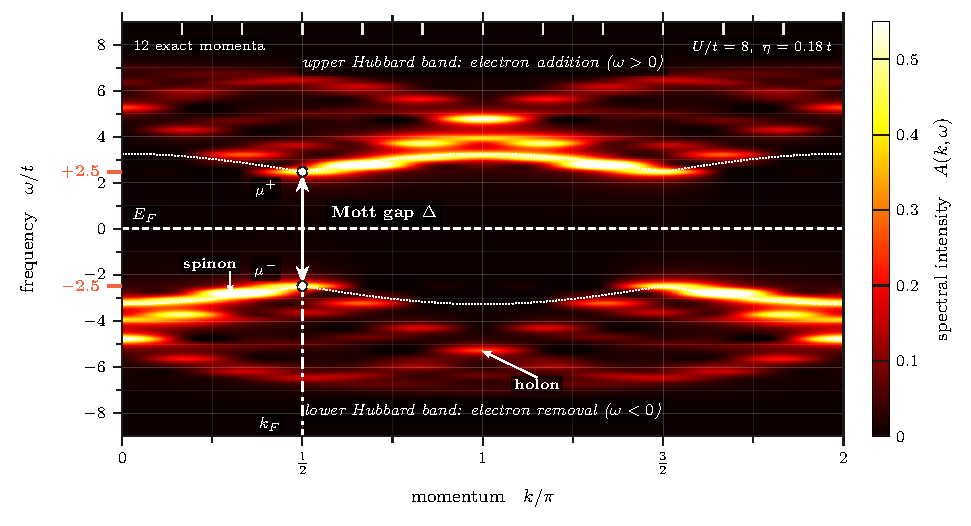
\includegraphics[width=\linewidth]{figs/fig_akw_native.pdf}
\caption{\textbf{Momentum-resolved spectral function: the dynamical target.} The
single-particle spectral function $A(k,\omega)$ of the half-filled Hubbard chain ($U/t=8$, $L=12$,
Lorentzian broadening $\eta=0.18\,t$), computed from the resolvent $\langle\phi|(z-\hat H)^{-1}|\phi\rangle$ by a
Haydock continued fraction~\cite{haydock1972} of depth $n_\ell=150$ over the full $(N{\pm}1)$ sectors---a
finite-depth continued fraction, that is a $150$-node Gauss quadrature of the spectral
measure~\cite{golub2010} and not the Lehmann sum; versions~1--2 called it exact and
Sec.~\ref{sec:physics} withdraws that word---the frequency- and momentum-resolved
observable that sample-based diagonalization targets but its energy-only output cannot itself deliver.
The two dispersing Hubbard bands---electron removal (lower, $\omega<0$; photoemission) and electron
addition (upper, $\omega>0$; inverse photoemission)---are separated by the correlation-driven
\emph{Mott gap} $\Delta=\mu^{+}-\mu^{-}=4.97\,t$ between the highest occupied state ($\mu^{-}$, lower
edge) and the lowest unoccupied state ($\mu^{+}$, upper edge), obtained from the exact $(N{\pm}1)$
ground-state energies (ticks at $\pm2.484\,t$); the broadened spectral peaks of the plotted $A(k_F,\omega)$
sit slightly wider, at $\pm2.49\,t$ (a $4.99\,t$ splitting), the $\sim\!0.02\,t$ excess being the
$\eta=0.18\,t$ Lorentzian broadening; the thermodynamic Lieb--Wu value~\cite{liebwu1968} is $4.68\,t$, the
$L=12$ excess being finite-size. The gap is \emph{direct} at the
Fermi momentum $k_F=\pi/2$. Particle--hole symmetry places the Fermi level at mid-gap ($\omega=0$),
verified to double-precision round-off, and each momentum obeys the analytic spectral sum rule
$\int A(k,\omega)\,d\omega=1$ (the plotted broadened grid recovers it to $\sim\!2\%$ within the $\pm9t$ window).
The lower Hubbard band is not a single quasiparticle branch but \emph{spin--charge separated}:
a narrow spinon branch (bandwidth $\pi J/2=0.79\,t$~\cite{descloizeaux1962}, $J=4t^2/U$; dashed,
validated against the exact peak dispersion to ${<}0.1\,t$) rides a broad holon (charge, ${\sim}4t$)
band---the hallmark fractionalization of the 1D Mott insulator~\cite{liebwu1968}. At $L=12$ that
structure is three to seven poles per momentum (Table~\ref{tab:poles}); the words appropriate to the
thermodynamic limit are not used for it.
The momentum axis is a periodic cubic-spline interpolation of the $12$ physical momenta (ticks, top).
Faithfully \emph{sampling} this full momentum-resolved observable---as opposed to the ground-state
energy---requires a large fraction of the $(N{+}1)$ sector (Fig.~\ref{fig:scaling}), the cost
quantified in Sec.~\ref{sec:prices}.}\label{fig:lattice}\end{figure*}


% =====================================================================================
%  Sec. 3 -- THE TWO BUDGETS.  The central theorem of the paper.  WRITTEN 2026-09-18.
%
%  This file did not exist until now.  thm:leakage, sec:leakage and eq:twobudget were
%  referenced 37, 17 and 7 times across the other nine sections and were defined
%  nowhere; app:counterex was referenced three times and defined nowhere.  All four
%  are defined here.
%
%  LABELS DEFINED HERE (and nowhere else):
%      sec:leakage  eq:lehmannA  eq:ritz3  eq:lambda  eq:twobudget  thm:leakage
%      eq:split  app:counterex
%  Sec. 3.1 (sec_3_1.tex, the retraction) is a SUBSECTION of this section and is
%  \input at the end of the [BODY] block.
%
%  PROVENANCE.  The statement, the three hypotheses and the numerical audit are those
%  adjudicated in P2_FRONTERA.md Sec. 4; the proof below is the one the evaluator
%  release/src/leakage_certificate.py realises, step for step, and its four rungs are
%  the four rungs whose contributions Sec. 5.5 measures (44 / 38 / 11 / 4.6 per cent).
%  The closed form of Lambda and the kernel 2 i eta / (Delta + 2 i eta) were re-derived
%  independently for this file by contour integration and agree with the form the code
%  evaluates.
%
%  VERIFIED FOR THIS FILE, on the 378 rows of the three deposited certificate scans
%  (release/data/cert_akw.json, cert_stress.json, cert_teqsci.json), by a script that
%  shares nothing with the one that wrote them:
%      - lower bound holds on 378 of 378;
%      - upper bound holds on 378 of 378; after removing the 2 rows that reproduce the
%        target to double-precision round-off (relative L1 <= 1e-10, where no ratio is
%        defined) the largest ratio error/bound is 0.9999999997;
%      - the exclusion lemma K_S >= 0 <=> w_S = 1 holds on 378 of 378, with 357 rows
%        at K_S = -1 and 21 at w_S = 1 exactly;
%      - the retracted bound of Sec. 3.1 fails on 219 of the 219 finite-ratio rows with
%        w_S >= 0.99, mildest factor 2.00, plus 19 rows where it is identically zero.
%
%  RESOLVED 2026-09-18: lowdin1962, feshbach1958 and saad2011 are in the bibliography and
%  were checked against Crossref (saad2011 is the SIAM *revised* edition, not a "2nd ed.").
%  This section additionally cites, since the novelty paragraph was rewritten:
%  paige1976, beattie2005, temple1928, weinstein1934, kato1949, frommersimoncini2008,
%  jialv2015, frommerschweitzer2016, oliveira2026 -- all present, all verified.
% =====================================================================================

% ======================================= [BODY] ======================================

\section{Two budgets: the missed weight and the boundary}
\label{sec:leakage}

The object a sample-based calculation delivers is a subspace, and the object a user wants is an error
bar on the response built inside it. This section proves the bound that connects them. It is two-sided,
it holds for \emph{any} orthogonal projector and therefore for any set of configurations a sampler
might return, and its upper branch separates into two terms with different economics: the first is fixed by the captured weight and vanishes once the probe's support is held; the second is not controlled by the weight, although it falls as the subspace grows. Everything after it is an evaluation of that
separation --- Sec.~\ref{sec:frontier} measures where the resulting certificate says something,
Sec.~\ref{sec:nogo} shows that no invariant of the state can replace it, and Sec.~\ref{sec:prices}
prices both terms in shots.

\subsection{The objects}

Fix the $(N{\pm}1)$ sector, let $H$ be the Hamiltonian restricted to it, $E_0$ the ground-state energy
of the $N$-electron sector, and let $\phi$ be the probe --- $\hat c^{\dagger}_p\ket{\Psi_0}$ or
$\hat c_p\ket{\Psi_0}$ for the charged channels, $\hat n_q\ket{\Psi_0}$ or $\hat S^{z}_q\ket{\Psi_0}$
for the neutral ones. Write $z=\omega+E_0+i\eta$ and $R(z)=(z-H)^{-1}$. The $\eta$-broadened spectral
function of Eq.~\eqref{eq:green} is
\begin{widetext}
\begin{equation}
A(\omega)\;=\;\frac{\eta}{\pi}\,\bigl\lVert R(z)\phi\bigr\rVert^{2},
\qquad\text{so that}\qquad
\int_{\mathbb R}A(\omega)\,d\omega\;=\;\lVert\phi\rVert^{2}
\label{eq:lehmannA}
\end{equation}
\end{widetext}
for every $\eta>0$, the sum rule holding because the Poisson kernel integrates to one on each Lehmann
pole. Let $P$ be an orthogonal projector on the sector, $Q=I-P$, and
\begin{widetext}
\begin{equation}
\phi_P=P\phi,\quad \phi_Q=Q\phi,\quad
w_P=\frac{\lVert\phi_P\rVert^{2}}{\lVert\phi\rVert^{2}},\quad
H_P=PHP,\quad R_P(z)=(z-H_P)^{-1}\big|_{\operatorname{ran}P},
\label{eq:ritz3}
\end{equation}
\end{widetext}
with Ritz pairs $H_P\ket{\tilde m}=\tilde E_m\ket{\tilde m}$ and $c_m=\braket{\tilde m|\phi}$. The
reconstruction of Eq.~\eqref{eq:ritz} is $A_P(\omega)=(\eta/\pi)\lVert R_P(z)\phi_P\rVert^{2}$, and it
obeys the same sum rule with $\lVert\phi_P\rVert^{2}$ on the right. When $P=P_{\mathcal S}$ is diagonal
in the determinant basis --- the only case a device produces --- we write $S$ for the configuration set
and $w_S$, $\Lambda_S$ for the quantities below.

The magnitude the theorem is indexed on is the Hamiltonian coupling that crosses the boundary of the
subspace, averaged over the resolution window rather than over the spectrum. With
$g_m=QH\ket{\tilde m}$,
\begin{widetext}
\begin{equation}
\Lambda_P(\eta)^{2}\;:=\;\frac{\eta}{\pi}\int_{\mathbb R}
\bigl\lVert QH\,R_P(z)\,\phi_P\bigr\rVert^{2}d\omega
\;=\;\sum_{m,m'}c_m\bar c_{m'}\,\braket{g_{m'},g_m}\,
\frac{2i\eta}{(\tilde E_{m'}-\tilde E_m)+2i\eta},
\label{eq:lambda}
\end{equation}
\end{widetext}
the second equality being exact and proved below; the sum is real, the $(m,m')$ and $(m',m)$ terms
being complex conjugates. Two features of Eq.~\eqref{eq:lambda} carry the practical content of this
paper. It is assembled from objects the reconstruction has already produced --- the Ritz vectors and
their coefficients --- plus one matrix--vector product $H\ket{\tilde m}$ per Ritz vector, so evaluating
it costs a small multiple of the diagonalization that produced $A_P$ and \emph{does not require} $A$.
And it vanishes exactly when $\operatorname{span}(S)$ contains $\mathcal K(H,\phi_P)$, the Krylov space of the retained part of the probe: $QHR_P(z)\phi_P$ vanishes for every $z$ exactly when $\mathcal K(H_P,\phi_P)$ is invariant under $H$, and it then coincides with $\mathcal K(H,\phi_P)$. For a subspace that holds the whole probe, $w_P=1$, the condition is that $\operatorname{span}(S)$ contain $\mathcal K(H,\phi)$ itself---far more demanding than it looks, as Sec.~\ref{sec:frontier:obstruction} measures.

\subsection{The bound}

\begin{theorem}[a posteriori leakage certificate]
\label{thm:leakage}
Let $H=H^{\dagger}$ act on the $(N{\pm}1)$ sector, let $\eta>0$, let $P$ be \emph{any} orthogonal
projector on that sector, and let $A$, $A_P$, $w_P$ and $\Lambda_P(\eta)$ be as in
Eqs.~\eqref{eq:lehmannA}--\eqref{eq:lambda}. Then
\begin{widetext}
\begin{equation}
\lVert\phi\rVert^{2}\bigl(1-w_P\bigr)
\;\le\;\lVert A-A_P\rVert_{1}\;\le\;
\min\Bigl\{\,\lVert\phi\rVert^{2}\bigl(1+w_P\bigr),\;
\bigl(\lVert\phi\rVert+\lVert\phi_P\rVert\bigr)
\bigl(\,\underbrace{\lVert\phi_Q\rVert}_{\text{missed weight}}
+\underbrace{\Lambda_P(\eta)/\eta}_{\text{boundary leakage}}\,\bigr)\Bigr\},
\label{eq:twobudget}
\end{equation}
% The restatement below used to sit in a SECOND widetext, with this clause as column
% text between the two.  That gave the output routine a legal break inside the theorem,
% and it took it: the hypothesis and Eq. (7) closed one page while the normalised form
% appeared on the next, behind Fig. 2 and its ten-line caption.  One widetext, no break
% point -- and two fewer horizontal rules on the page.
\noindent equivalently, dividing by $\lVert\phi\rVert^{2}$ and writing
$\widehat\Lambda_P=\Lambda_P/\lVert\phi\rVert$,
\begin{equation*}
1-w_P\;\le\;\frac{\lVert A-A_P\rVert_{1}}{\lVert\phi\rVert^{2}}\;\le\;
\min\Bigl\{\,1+w_P,\;\bigl(1+\sqrt{w_P}\bigr)
\bigl(\sqrt{1-w_P}+\widehat\Lambda_P(\eta)/\eta\bigr)\Bigr\}.
\end{equation*}
\end{widetext}
\end{theorem}


\noindent Three hypotheses carry it, each a property of the \emph{pipeline} that produced $A_P$ rather
than of the inequality: \emph{(H1)} $A$ and $A_P$ are referred to the same $E_0$; \emph{(H2)} the $L_1$
norm is taken over the whole line and normalized by $\lVert\phi\rVert^{2}$; \emph{(H3)} $A$ is the exact
spectral function of the full sector. Each is load-bearing and each is checked against this paper's own
pipeline in Sec.~\ref{app:hyp}; the proof, from the Feshbach--L\"owdin split of the resolvent
(Eq.~\eqref{eq:split}) and Cauchy--Schwarz in $\omega$, is in Sec.~\ref{sm:leakage}.

\subsection{What the two branches are, and what they are not}

\paragraph{What the weight does not control.} The first summand of the leakage branch, $\lVert\phi_Q\rVert=\lVert\phi\rVert\sqrt{1-w_P}$, is the Born weight of the probe the subspace failed to hold: it vanishes once the sampler holds the probe's Born support, and Table~\ref{tab:provenance} prices that purchase channel by channel. The second, $\Lambda_P(\eta)/\eta$, reads the off-diagonal block $PHQ$, and the captured weight does not control it: along the sampler's ranking it falls as $S$ grows (Sec.~\ref{sec:frontier}), but a subspace can hold the whole probe and still leak. Section~\ref{sec:retraction} turns this from a reading into a measurement: on
$\mathcal S^{\star}=\operatorname{supp}(\phi)$, where the first summand vanishes identically and by
construction, the relative $L_1$ error remains of order one, against a ceiling of $2$.

\paragraph{A certificate, not an error estimate.} The gap between the bound and the measured error is
large, and it is not the accident of a constant. At \emph{fixed} $P$ the looseness is stable --- within
$\pm17\%$ ($L=6$) and $\pm25\%$ ($L=8$) over a decade in $\eta$ --- but across subspaces it varies by a
factor $51$, and at the threshold where the leakage branch first improves on the trivial one it is
$3\times10^{2}$ to $2.4\times10^{3}$ (Sec.~\ref{sec:frontier:calib}). Eq.~\eqref{eq:twobudget} is therefore an exclusion, not an error
estimate; Sec.~\ref{sec:frontier} reports what it excludes, and at what fraction of the sector.

\paragraph{Only one of the two terms is a posteriori.} $\Lambda_P(\eta)$ is computable from $H$,
$\operatorname{ran}P$, $\phi$ and the Ritz vectors alone. The weight term is not: $w_P$ needs the exact
decomposition of the probe norm, and estimating it against an already-truncated $\Psi_0$ is biased in
the optimistic direction. The complete bound is therefore \emph{not} evaluable by a user who does not
already have the answer, and we never claim that it is; Sec.~\ref{sec:frontier:calib} gives the
conservative substitution that makes the decision itself a posteriori in the regime where it is used.

\paragraph{Prior art, and what is new.} Nothing in the proof is new as analysis. The split is L\"owdin
partitioning~\cite{lowdin1962}, the algebra of the Feshbach projection~\cite{feshbach1958}; Rayleigh--Ritz
and Krylov error analysis for resolvents and matrix
functions~\cite{saad2011,golub2010,epperly2022,temple1928,weinstein1934,kato1949,paige1976,beattie2005}
contains every rung of its steps, and the integration step is the reduced-basis bound on a Galerkin
projection with inf--sup constant $\eta$~\cite{rozza2008,hesthaven2016}. A posteriori estimates for Krylov
approximations to matrix functions are due to Frommer and Simoncini, Jia and Lv, and Frommer and
Schweitzer~\cite{frommersimoncini2008,jialv2015,frommerschweitzer2016}, with Lanczos and
stochastic-Lanczos-quadrature versions~\cite{chen2022lanczos,xuchen2025block,chen2021slq}; on quantum
Krylov, Oliveira, Ziems and Glaser assess reliability without knowledge of the true
spectrum~\cite{oliveira2026}; and a response-targeted selection criterion for classical selected
configuration interaction is Reinholdt, Kjellgren and Kongsted's~\cite{reinholdt2026lr}. The priority
for the a posteriori framing is theirs. What we add is the conjunction of three things: a closed form
for $\Lambda_P(\eta)$ from the Ritz pairs on a subspace of \emph{coordinates}, with no Krylov structure,
invariance or gap assumption; a bound two-sided on the same object; and a measured calibration of where
it crosses the trivial bound (Sec.~\ref{sec:frontier:calib}). Whether it is useful at the fractions
sampling reaches is answered, in the negative, in Sec.~\ref{sec:frontier}; the full comparison with that
literature is in Sec.~\ref{sm:leakage}.

% =====================================================================================
%  Sec. 3.1 -- Retraction of Theorem 1(iii).  Goes INSIDE Sec. 3 (Theorem B), in the body.
%  Supersedes: theorem_b2.tex lines 45-49 (the (iii) statement) and the (iii) clause of
%              the proof sketch, theorem_b2.tex lines 60-65;
%              method.tex lines 82-88 ("the genuine certificate ...");
%              discussion.tex lines 32-36 ("its error is bounded by the captured spectral weight").
%  Drop-in replacements for the latter two are appended, commented out, at the end of this file.
%
%  EXTERNAL LABELS USED HERE (must exist in the v3 tree -- see the report):
%    thm:leakage    Theorem B, the two-sided replacement            [Sec. 3, new; agreed]
%    sec:frontier   where the certificate's non-vacuity is mapped   [Sec. 5, new; agreed]
%    sec:moments    moment exactness, the surviving part (i)        [Sec. 4, defined in sec_4.tex]
%    sec:nogo       the orbital-invariance obstruction              [Sec. 6, defined in sec_6.tex]
%    app:counterex  counterexamples + the 292-subspace sweep        [Appendix B, NOT YET DEFINED]
%    fig:violation  new Fig. N3, violation vs fraction and vs eta   [Appendix B, NOT YET DEFINED]
%    sec:prices     the three prices                                [Sec. 7, defined in sec_7.tex]
%    tab:fracgrid   frac(L,eta) grid                                [Sec. 7, defined in sec_7.tex]
%    sec:method, sec:honest, fig:akwsampled, fig:scaling            [already in the tree]
%  This file defines only sec:retraction, eq:weightonly, eq:exclusion, eq:mu2.
%  Sec. 3's own label is sec:leakage -- agreed across sec_4.tex, sec_6.tex and sec_7.tex.
%  The obsolete alternative "sec:budgets" is used NOWHERE; do not reintroduce it.
%  NO \cite key exists for this preprint itself; arXiv:2608.16436 is given in prose.
%
%  %TODO(Sec. 3): three hypotheses of Theorem B are NOT stated in this file because they belong to
%  the theorem's own statement, which Sec. 3 owns.  They are load-bearing and a referee finds them by
%  reading step (1) of the proof.  They must appear in the statement, not in a reply:
%    (a) the published relative L1 is normalized by the in-window integral of |A_exact|, not by
%        ||phi||^2 (inflation ~1.027 at L=8);
%    (b) the "exact" reference of the resource scan is recomputed at the SAME n_l as the subspaces,
%        so the published relative L1 is ||A_K^full - A_K^S||, not ||A - A_K^S||;
%    (c) the theorem assumes A and A_P share E_0.  In the flagship point an origin error of
%        3.5e-4 t alone reproduces the whole certified error, and in a real shot-based pipeline E_0 is
%        itself estimated on a sampled subspace.  It has never been tested that way.
% =====================================================================================

\subsection{The captured weight is not the controlling magnitude}
\label{sec:retraction}

The certificate one would want for a sampled reconstruction indexes the error on the captured
weight alone,
\begin{equation}
\lVert A-A_S\rVert_{1}\;\le\;2\lVert\phi\rVert^{2}(1-w_S)\;+\;C\,\rho^{-K_S},
\label{eq:weightonly}
\end{equation}
with $w_S=\lVert P_S\phi\rVert^{2}/\lVert\phi\rVert^{2}$ and $K_S$ the largest Krylov order
contained in $\operatorname{span}(S)$ (we set $K_S=-1$ when $\phi\notin\operatorname{span}(S)$).
It is false, for every constant $C$ and every $\rho$, and it fails hardest in exactly the regime
a sampling experiment aims for. 

\paragraph{A two-level counterexample forces the trivial constant.}
Take $H=\big(\begin{smallmatrix}0&g\\ g&0\end{smallmatrix}\big)$, $\phi=e_0$, $S=\{0\}$, $E_0=0$. Then
$P_S\phi=\phi$, so $w_S=1$ exactly and the weight term vanishes identically; and
$\mathcal K_0=\operatorname{span}\{\phi\}\subseteq\operatorname{span}(S)$ while
$\mathcal K_1\not\subseteq\operatorname{span}(S)$, so $K_S=0$ exactly and the second term is the bare
constant $C$. The exact $A$ is a pair of Lorentzians of weight $\tfrac12$ at $\pm g$; the
reconstruction, built on $H_S=P_SHP_S=0$, is one Lorentzian of weight $1$ at the origin, so
$\lVert A-A_S\rVert_{1}\to2\lVert\phi\rVert^{2}$ as $g/\eta\to\infty$. Since $g$ is free,
\eqref{eq:weightonly} requires $C\ge2\lVert\phi\rVert^{2}$: false if $C$ is a constant, vacuous if it may depend on the instance. The same holds at every Krylov order: on a chain of $K+2$ sites with $\phi=e_0$ and $S$ its first $K+1$ sites, $w_S=1$ and $K_S=K$, and the exact and reconstructed spectra have strictly interlacing poles, so the same limit requires $C\rho^{-K}\ge2\lVert\phi\rVert^{2}$ for every $K$, which no fixed $C$ satisfies when $\rho>1$. With $w_S<1$ strictly the weight term alone fails without bound: in a three-level family its violation diverges as $\varepsilon^{-2}$ in the amplitude $\varepsilon$ of the discarded component (Sec.~\ref{app:counterex}). By contrast
$\lVert A-A_S\rVert_{1}\le\lVert\phi\rVert^{2}(1+w_S)$ holds for every $S$ under no hypothesis at all,
$A$ and $A_S$ being nonnegative with known integrals: that trivial bound is the only surviving member of
the family \eqref{eq:weightonly}, and Theorem~\ref{thm:leakage} keeps it explicitly, as the first branch
of its minimum.
\paragraph{The violation is systematic, and worst where the reconstruction is best.} In a pooled sweep
of $606$ subspaces from five Hamiltonian families the weight-only bound fails on $468$, and on all $363$
with $w_S\ge0.99$, the mildest by a factor $2.10$ (Fig.~\ref{fig:thm1iii-violation}); in a
first sweep it failed on $126$ of $126$ such subspaces. In the
configuration of Fig.~\ref{fig:akwsampled} its median violation factor rises from $18.5$ to $29.9$
between sector fractions $0.50$ and $0.95$ while the measured error falls by three orders of magnitude.
The sweep and its declared limits are in Sec.~\ref{sm:leakage}; the conclusion does not depend on it,
the counterexample being analytic.

\paragraph{Why it fails.} The reconstruction is Rayleigh--Ritz on $H_S=P_SHP_S$, not a restriction of
$A$ to a subset of its eigenpairs: weight the subspace keeps is \emph{displaced} in $\omega$, not
discarded, and the two-level example is the extreme case. What the integrals do give is the lower bound
$\lVert\phi\rVert^{2}(1-w_S)\le\lVert A-A_S\rVert_{1}$, with $0$ violations across the $606$ subspaces,
the left-hand half of Theorem~\ref{thm:leakage}.

\paragraph{The two terms are mutually exclusive, and one is off at every operating point here.}
$S$ is a set of determinants, so $P_S$ is diagonal in the working basis and
$P_S\phi=\phi\iff\operatorname{supp}(\phi)\subseteq S\iff w_S=1$, while $K_S\ge0$ means precisely
$\phi=H^{0}\phi\in\operatorname{span}(S)$. Hence the exclusion lemma
\begin{equation}
K_S\ \ge\ 0\qquad\Longleftrightarrow\qquad w_S\ =\ 1 ,
\label{eq:exclusion}
\end{equation}
verified with $0$ discrepancies across the $378$ deposited subspaces, of which $357$ have $K_S=-1$ (Sec.~\ref{app:counterex}). The two terms of
\eqref{eq:weightonly} are therefore never both informative: either $w_S=1$ and the whole bound is the
second term --- the two-level counterexample --- or $K_S=-1$ and $C\rho^{-K_S}=C\rho$, an undefined
constant with no decay in it. Counting settles which branch applies here. The seed is
$\phi=\hat c^{\dagger}_{0\uparrow}\ket{\Psi_0}$ at half filling, so $\operatorname{supp}(\phi)$ lies in the set of $(N{+}1)$ determinants with orbital $0\!\uparrow$ occupied, a fraction $n_\uparrow/L=\tfrac12+\tfrac1L$ of the sector, and fills it except where symmetry zeroes an amplitude of $\Psi_0$. By \eqref{eq:exclusion}, $K_S\ge0$ demands $|S|\ge\lvert\operatorname{supp}(\phi)\rvert$, a floor of $0.571$ at $L=8$ ($2237$ of $3920$), $0.600$ at $L=10$, and above $0.54$ at $L=12$ and $14$ at any amplitude threshold from $10^{-12}$ to $10^{-10}$, against the sector fractions $0.5561$, $0.3625$, $0.1700$, $0.0800$
at which the resource scan of Sec.~\ref{sec:prices} operates (Fig.~\ref{fig:scaling}; the coarser
replication grid of Table~\ref{tab:fracgrid} reads $0.180$ at $L=12$ for the same operating point).
From $L=8$ on, every operating point of that scan lies below its own floor, so $K_S=-1$ by counting
alone, with no
numerics, no ranking and no protocol, and any point below the same line inherits the verdict
(Sec.~\ref{app:counterex}). 
Theorem~\ref{thm:leakage} carries no such
bookkeeping and is held to the opposite standard. Its two terms are defined and simultaneously active
for every $S$; the weight term is the half this work cannot compute without $\Psi_0$ ---
$\lVert\phi_Q\rVert=\lVert\phi\rVert\sqrt{1-w_S}$, and estimating $w_S$ against an already-truncated
$\Psi_0$ is biased optimistically --- while $\Lambda_S(\eta)$ is an \emph{a posteriori} quantity
assembled from the Ritz vectors the reconstruction already forms plus one matrix--vector product, and is
evaluated, subspace by subspace, in Sec.~\ref{sec:frontier}.

\paragraph{The magnitude, not the constant.}
Two measurements at the same, exactly unit, captured weight show that \eqref{eq:weightonly} was indexed
not on a bad constant but on the wrong quantity. First, let $S^\star=\operatorname{supp}(\phi)$, the
smallest determinant subspace of unit captured weight --- fixed by the seed, with no ranking, no
tie-breaking and no zero-amplitude padding --- of size $(\tfrac12+\tfrac1L)D$ at $L=6$ and $0.571\,D$ at $L=8$, where $426$ of the $4900$ ground-state amplitudes vanish by symmetry. Its weight term
is identically zero, and its relative $L_1$ error is $0.43$ at $L=6$ and $0.35$ at $L=8$ on the periodic rings at $\eta=0.18t$, rising to $1.15$ and $0.73$ at $\eta=0.05t$, against a hard ceiling of $1+w_S=2$.
Second, $S^\star$ is the $K=0$ rung of the Krylov ladder
$S_K=\bigcup_{a\le K}\operatorname{supp}(H^{a}\phi)$, every rung of which contains $\phi$ and so carries
$w_S=1$ identically, while its moment reach grows: $S_K$ reproduces the exact spectral moments through
order $2K{+}1$ --- to the $10^{-15}$ level, failing as it must at $2K{+}2$ --- whereas coordinate
subspaces of the same size drawn at random miss already $\mu_0$, in all of $300$ draws
(Sec.~\ref{sec:moments}). Along a family of constant, exactly unit captured weight the error therefore
runs from order unity to moment-exact through order $2K{+}1$. The captured weight, identical on every
rung, does not order them.

What does is elementary. Writing $\mu_j,\mu^{S}_j$ for the moments of the unbroadened measures of
Sec.~\ref{sec:moments}, every determinant subspace with $w_S=1$ reproduces $\mu_0$ and $\mu_1$ exactly,
and the first moment that can fail is $\mu_2$, with deficit
\begin{equation}
\mu_2-\mu^{S}_2\;=\;\lVert Q_S H P_S\phi\rVert^{2},\qquad Q_S=I-P_S ,
\label{eq:mu2}
\end{equation}
the squared coupling of the Hamiltonian across the boundary of $S$ ($E_0$ drops out because
$Q_S\phi=0$), zero exactly when $S$ also holds $\operatorname{supp}(H\phi)$ --- the $K_S\ge1$ condition.
That boundary coupling is the magnitude the replacement is indexed on: it controls the leakage term
through $\Lambda_S(\eta)\le\lVert P_SHQ_S\rVert\,\lVert\phi_S\rVert$, and Theorem~\ref{thm:leakage}
averages it over the resolution window rather than over the spectrum. The captured weight says what the
subspace \emph{contains}; the error is set by what the Hamiltonian does to the seed at the subspace's
\emph{edge}. Both halves of this paper follow from that displacement: Sec.~\ref{sec:frontier} measures
where the boundary term is small enough for the certificate to say something, and Sec.~\ref{sec:nogo}
shows why no orbital-rotation invariant can predict it in advance.

% =====================================================================================
%  DROP-IN REPLACEMENTS FOR THE TWO SURVIVING INVOCATIONS (not part of Sec. 3.1;
%  move into the target files -- do not compile from here).
%
%  (1) method.tex, replacing the sentence at lines 82-88 ("These zeroth-moment checks are not
%      themselves an error bound; the genuine certificate is ... (Sec.~\ref{sec:honest})."):
%
% These zeroth-moment checks are not themselves an error bound. The certificate is the two-sided
% bound of Theorem~\ref{thm:leakage}, which splits the $L_1$ error into the Born weight the subspace
% failed to capture and the Hamiltonian coupling leaking across its boundary at resolution $\eta$;
% only the first of the two is bought by drawing more bitstrings. A weight-only bound appeared in
% versions~1 and~2 of this preprint and is retracted in Sec.~\ref{sec:retraction}. Where the
% certificate is non-vacuous is measured, not asserted, in Sec.~\ref{sec:frontier} --- an essential
% property given that the classical hardness of a specific instance is empirical rather than a
% theorem (Sec.~\ref{sec:honest}).
%
%  (2) discussion.tex, replacing lines 32-36 ("On the positive side, Theorem~\ref{thm:b2}
%      (Sec.~\ref{app:b2}) guarantees ... bounded by the captured spectral weight."):
%
% On the positive side, moment exactness (Sec.~\ref{sec:moments}) guarantees that a subspace
% containing the order-$K$ Krylov space reproduces the exact spectral moments through order $2K{+}1$
% and is captured with a polynomial shot budget, and Theorem~\ref{thm:leakage} certifies the
% reconstruction two-sidedly: from below by the captured weight, from above by that weight together
% with the boundary leakage. The error is \emph{not} bounded by the captured spectral weight alone ---
% a subspace holding the entire Born support of the seed, of unit weight by construction, still
% carries a relative $L_1$ error of $0.28$ to $0.43$ at $\eta=0.18t$, the lower end on the open chain
% of the method validation and the upper on the periodic ring (Sec.~\ref{sec:retraction}).
%
%  INTEGRATION NOTE: after these two replacements are made, \ref{thm:b2} must appear NOWHERE in the
%  live tree.  Its parts (i) and (ii) become Theorem~\ref{thm:moments} and Prop.~\ref{prop:shots}
%  (Sec. 4), its part (iii) is retracted here, and its corollary becomes Conjecture~\ref{conj:geom}.
%  The only occurrence of the string thm:b2 in this file is inside the quotation above, which is the
%  OLD sentence being replaced.
% =====================================================================================





% =====================================================================================
% Sec. 4 -- WHAT THE STRUCTURE DOES CERTIFY: MOMENT EXACTNESS
%
% Replaces, in paper/theorem_b2.tex: the statement of Theorem 1 parts (i) and (ii)
% (lines 18-50, up to the start of part (iii)), the proof sketch of (i) and (ii)
% (lines 52-60), and the composition paragraph (lines 68-76).
% Part (iii) is retracted in sec_3_1.tex and does not appear here.
%
% This file contains TWO blocks, separated by the marked rule below:
%   [BODY]     -> main body, after Sec. 3 (the two budgets / Theorem B).
%   [APPENDIX] -> after \appendix, replacing the first appendix of theorem_b2.tex.
%
% External labels used here (owned by other sections -- reconcile at integration):
%   sec:leakage    = Sec. 3, the two-budget decomposition   [label spelling taken from sec_6.tex]
%   thm:leakage    = Theorem B, the leakage bound           [Sec. 3, agreed across sections]
%   sec:retraction = Sec. 3.1, retraction of Thm 1(iii)     [defined in sec_3_1.tex]
%   sec:frontier   = Sec. 5, where the certificate is non-vacuous  [Sec. 5, not yet written]
%   sec:prices     = Sec. 7, the three prices               [defined in sec_7.tex]
%   eq:supportexp  = |S| ~ e^{1.05 L}                       [defined in sec_7.tex]
%   sec:method     = Sec. 2                                 [label already exists in method.tex]
% This file defines: sec:moments, sec:moments:exact/notbuy/shots, thm:moments, conj:geom,
%   prop:shots, tab:moments, eq:momex, eq:rrsplit, eq:shots, app:moments(+:exact/sharp/conj/shots).
%
% PROVENANCE.  Table~\ref{tab:moments}: rows K=0,1 from p2_texto/final_out.txt (six independent
%   implementations), row K=2 from p2_texto/bc2_out.txt (the corrected run; see app:moments:sharp
%   for why the earlier one is discarded).  Negative control: p2_texto/control_out.txt, 300 draws,
%   seed 20260918.  Two-level toy series of app:moments:conj: p2_texto/toy_out.txt.  The rho ~ 1.7
%   paragraph of sec:moments:notbuy: release/data/method_max.json (shots=4000, NSEEDS=8, dt=0.4)
%   and release/src/spectral_validation_max.py:225.
% *** DEPOSIT GAP, corrected and escalated 2026-09-21.  This note used to read "the four .txt
%   artifacts above live in the author's working tree, NOT in release/".  That was too kind and
%   is now false: the four .txt files AND the four scripts that produced them (verify_final.py,
%   verify_bc2.py, verify_control.py, verify_toy.py) exist NOWHERE -- searched across release/
%   and the whole working tree on 2026-09-21.  Table~\ref{tab:moments} and the negative control
%   are therefore not regenerable from the deposit.
%
%   That fact is no longer left to this comment, because arXiv publishes the LaTeX source and a
%   limitation a reader can only find by downloading the .tex is a limitation that was hidden.
%   It is now declared where this project declares gaps: COVERAGE_GAP_V3 in src/verify.py, which
%   prints it by name on every run, and docs/DATA_AVAILABILITY.md.
%
%   It is also cheap to close, and closing it is the real fix: the table is L = 6, sector
%   dimension 300, exact diagonalization of the (N+1, Sz=+1) sector (see sec_4_app.tex:53).
%   Rewrite the four scripts against that construction, deposit them with their outputs, and
%   assert the three rows in verify.py.  release/data/method_max.json, which the rho ~ 1.7
%   paragraph uses, IS deposited and is unaffected. ***
% =====================================================================================

% `conjecture' environment, declared defensively so this file can be dropped in whether
% or not main.tex already declares one.
\makeatletter
\@ifundefined{c@conjecture}{\newtheorem{conjecture}{Conjecture}}{}
\makeatother

% ======================================= [BODY] ======================================

\section{What the structure does certify: moment exactness}
\label{sec:moments}

Section~\ref{sec:retraction} rules out an error bound indexed on the captured weight. It rules out nothing about the construction itself. One structural guarantee does hold, and
it is the one that says what a Krylov-adequate subspace actually buys: a finite list of spectral
moments, exactly. We state it with the proof the code realizes, measure its exact reach, and separate
it from two claims that attach themselves to it and do not follow from it.

\subsection{The statement that survives, and the proof it actually has}
\label{sec:moments:exact}

Write $\mathcal K_K=\operatorname{span}\{\phi,H\phi,\dots,H^{K}\phi\}$ for the order-$K$ Krylov space
of the seed $\ket{\phi}=\hat c^{\dagger}_{p}\ket{0}$, and let $d\mu$ and $d\mu_{\mathcal S}$ be the
unbroadened Stieltjes measures whose Lorentzian convolutions are the exact $A$ and the reconstruction
$A_{\mathcal S}$, the Lehmann sum evaluated inside $\operatorname{span}(\mathcal S)$ as in
Sec.~\ref{sec:method} (Sec.~\ref{app:moments}).

\begin{theorem}[Moment exactness]
\label{thm:moments}
Let $P$ be the orthogonal projector onto $\operatorname{span}(\mathcal S)$ and $H_{\mathcal S}=PHP$.
If $\operatorname{span}(\mathcal S)\supseteq\mathcal K_K$, then
\begin{widetext}
\begin{equation}
\int \omega^{j}\,d\mu_{\mathcal S}(\omega)\;=\;\int \omega^{j}\,d\mu(\omega)
\;=\;\braket{\phi|(H-E_0)^{j}|\phi},\qquad 0\le j\le 2K+1 .
\label{eq:momex}
\end{equation}
\end{widetext}
\end{theorem}

\begin{proof}
Because $\mathcal K_K\subseteq\operatorname{span}(\mathcal S)$ we have $PH^{a}\phi=H^{a}\phi$ for
$0\le a\le K$, whence by induction $H_{\mathcal S}^{\,b}\phi=P H^{b}\phi$ for $0\le b\le K+1$. Then for
any $a\le K$ and $b\le K+1$, using only $P=P^{\dagger}=P^{2}$ and $H=H^{\dagger}$,
\begin{widetext}
\begin{equation}
\braket{\phi|H_{\mathcal S}^{\,a+b}|\phi}=\braket{H_{\mathcal S}^{\,a}\phi|H_{\mathcal S}^{\,b}\phi}
=\braket{H^{a}\phi|P H^{b}\phi}=\braket{P H^{a}\phi|H^{b}\phi}=\braket{\phi|H^{a+b}|\phi},
\label{eq:rrsplit}
\end{equation}
\end{widetext}
and every $j\le 2K+1$ is such an $a+b$. Both measures are shifted by the same $E_0$, so the identity
survives term by term in the binomial expansion of $(H-E_0)^{j}$.
\end{proof}

\noindent The proof is three lines of Rayleigh--Ritz. It does not identify $A_{\mathcal S}$ with a
Gaussian-quadrature rule, which is not the object built here: every reconstruction diagonalizes
$P_{\mathcal S}HP_{\mathcal S}$ on a coordinate subspace, so $d\mu_{\mathcal S}$ carries
$|\mathcal S|$ nodes, not $K+1$ (Sec.~\ref{sm:moments}).

Table~\ref{tab:moments} measures Eq.~\eqref{eq:momex} on the construction this work uses---the union of
the determinant supports of $\{\phi,H\phi,\dots,H^{K}\phi\}$---for the open Hubbard chain at $L=6$,
$U/t=8$, in the $(N{+}1,S_z{=}{+}1)$ sector of dimension $D=300$. Through order $2K+1$ the moments
agree to a relative $10^{-14}$; at order $2K{+}2$ they part company by eleven orders of magnitude at
$K=0$ and seven at $K=1$. The order $2K+1$ is the exact reach of the construction, not merely a
sufficient claim, and the two rows that exhibit that reach are the two on which the ladder has not yet
filled the sector.

\begin{table*}[tp]\centering\small
\caption{\textbf{Moment exactness and its exact reach.} Open Hubbard chain, $L=6$, $U/t=8$; seed
$\ket{\phi}=\hat c^{\dagger}_{0\uparrow}\ket{0}$; $(N{+}1,S_z{=}{+}1)$ sector of dimension $D=300$;
$\mathcal S=\bigcup_{a\le K}\operatorname{supp}(H^{a}\phi)$. The largest Krylov order inside
$\operatorname{span}(\mathcal S)$, $K_{\mathcal S}$, and the captured Born weight $w_{\mathcal S}$ are
measured, not assumed. $\epsilon_j$ is the \emph{relative} discrepancy of the $j$-th moment, quoted as
the largest value over six equivalent implementations of the same identity; the absolute discrepancy at
order $2K{+}2$ follows in parentheses. Only relative residues are quoted below that order, because
$\mu_j$ spans five decades between $j=0$ and $j=6$ and the absolute roundoff residue is
route-dependent (Sec.~\ref{app:moments:sharp}). At $K=2$ the ladder has filled the sector, so
$\operatorname{span}(\mathcal S)$ carries every eigenvector of nonzero Lehmann weight,
$A_{\mathcal S}=A$ identically, and there is no order-$2K{+}2$ failure to exhibit; that row is kept to
mark where the ladder terminates, and its single entry is the roundoff level of the moments.}
\label{tab:moments}
\begin{tabular}{cccccc}\hline\hline
$K$ & $|\mathcal S|$ & $|\mathcal S|/D$ & $w_{\mathcal S}$ & $K_{\mathcal S}$ &
$\max_{j\le 2K+1}\epsilon_j\ \longrightarrow\ \epsilon_{2K+2}$ (absolute) \\ \hline
$0$ & $200$ & $0.667$ & $1$ & $0$ &
$1.8\times10^{-15}\ \longrightarrow\ 9.5\times10^{-4}$\ \ $(3.10\times10^{-2})$ \\
$1$ & $280$ & $0.933$ & $1$ & $1$ &
$3.2\times10^{-15}\ \longrightarrow\ 6.0\times10^{-8}$\ \ $(1.34\times10^{-4})$ \\
$2$ & $300$ & $1.000$ & $1$ & full sector &
$7.5\times10^{-15}\ \longrightarrow\ $ no failure: $A_{\mathcal S}=A$ \\
\hline\hline\end{tabular}
\end{table*}

A negative control fixes what the table is about. Over $300$ coordinate subspaces of the \emph{same}
size $|\mathcal S|=200$---two thirds of the sector---drawn uniformly from it, every single draw fails
already at the zeroth moment, against $4\times10^{-16}$ for the Krylov-support subspace of identical
size (Sec.~\ref{app:moments:sharp}). What
Theorem~\ref{thm:moments} certifies is \emph{which} determinants the subspace holds, not \emph{how
many}---a structural property, decidable from the subspace alone, before any exact reference exists.

One caveat of scale belongs with the table. The ladder terminates once the subspace contains the cyclic
subspace generated by $\phi$, and there the reconstruction is exact: at $L=6$ that is $K=2$ on the open
chain, and already $K=1$ on the periodic rings of Sec.~\ref{sec:prices}, where it stalls at $296$ of
$300$ determinants with $A_{\mathcal S}=A$ to $10^{-14}$ (Sec.~\ref{app:moments:sharp}). Three rows is
all this validation system has, and we claim nothing about the large-$K$ behaviour of
$\lVert A-A_{\mathcal K_K}\rVert_1$. Within the reach it covers, the identity is exact and sharp at the
next order.

\subsection{What moment exactness does not buy}
\label{sec:moments:notbuy}
Moment exactness is a list of $2K+2$ linear identities, and the $L_1$ distance between two
Lorentzian-broadened measures is not a finite linear functional of them, so geometric convergence in the
Krylov order does not follow from it. We state that claim as what it is.

\begin{conjecture}[Geometric convergence in the Krylov order]
\label{conj:geom}
Fix $\eta>0$ and let $A_{\mathcal K_K}$ be the Rayleigh--Ritz reconstruction on $\mathcal K_K$. Are
there $C(\eta)<\infty$ and $\rho(\eta)>1$, uniform over a class of Hamiltonians containing the models
studied here, such that $\lVert A-A_{\mathcal K_K}\rVert_{1}\le C(\eta)\,\rho(\eta)^{-K}$ for every
$K$?
\end{conjecture}

\noindent The two-level family of Sec.~\ref{sec:retraction} already forces $C(\eta)\ge2\lVert\phi\rVert^{2}$
at $K=0$, so any content the conjecture has must be carried by $\rho(\eta)^{-K}$ alone. Nor is
Eq.~\eqref{eq:momex} an error bound: for a coordinate subspace, containing $\mathcal K_K$ forces
$w_{\mathcal S}=1$, and at unit captured weight the error is $O(1)$---$0.28$ on the open chain of
Table~\ref{tab:moments} at $\eta=0.18\,t$, and up to $0.43$ on the periodic rings
(Sec.~\ref{sec:leakage}). The panel of Fig.~\ref{fig:method} read against the conjecture, and the full
discussion, are in Sec.~\ref{sm:moments}.

\subsection{The shot count}
\label{sec:moments:shots}

Proposition~\ref{prop:shots} counts the shots that populate such a subspace. Bitstrings are
drawn from the time-averaged Born mixture
$p(x)=\tfrac{1}{K+1}\sum_{k=0}^{K}\lvert\braket{x|e^{-iHt_k}\phi}\rvert^{2}/\lVert\phi\rVert^{2}$, and
the target is to capture every configuration with $p(x)\ge\varepsilon$ at confidence $1-\delta$. The natural answer, $T=O(\varepsilon^{-1}\log(|\mathcal S|/\delta))$, is circular:
$|\mathcal S|$ is the random output of the very $T$ draws the bound is meant to fix.

A non-circular form costs nothing. With $\mathcal N_\varepsilon=\{x:p(x)\ge\varepsilon\}$, each member contributing at
least $\varepsilon$ to a probability distribution, $|\mathcal N_\varepsilon|\le1/\varepsilon$
\emph{deterministically}; a union bound over $\mathcal N_\varepsilon$ of the event ``$x$ never drawn in
$T$ trials'' then gives
$\Pr[\mathcal N_\varepsilon\not\subseteq\mathcal S]\le\varepsilon^{-1}e^{-\varepsilon T}$, so
\begin{equation}
T\;\ge\;\varepsilon^{-1}\log\!\bigl(1/(\varepsilon\delta)\bigr)
\label{eq:shots}
\end{equation}
suffices (Prop.~\ref{prop:shots}). This is non-circular, and wherever the sampler returns more than
$\varepsilon^{-1}$ distinct configurations its logarithm is the smaller of the two as well.

The parameter $\varepsilon$ thresholds a Born probability, not a spectral accuracy: even at
$w_{\mathcal S}=1$ the error is $O(1)$, so capturing the high-probability configurations is a statement
about the sampler, not about the spectrum; what the resulting subspace costs is priced in
Sec.~\ref{sec:prices} (Sec.~\ref{sm:moments} gives the two compositions of the bound this work does not
make).



% =====================================================================================
%  Sec. 5 -- WHAT THE CERTIFICATE CAN AND CANNOT ASSERT:
%            THE NON-VACUITY THRESHOLD OF THE LEAKAGE BOUND
%
%  NEW section; no predecessor in the v2 tree.  It resolves the live internal contradiction
%  between discussion.tex:55-58 ("demands a large fraction of the sector") and
%  results.tex:253-256 ("falls to 8 per cent"), today two opposite arguments in one paper.
%
%  This file contains TWO blocks, separated by the marked rule near the end, on the pattern
%  sec_4.tex already uses:
%    [BODY]     -> main body, after Sec. 4.  Measured: 4.1 pages at the main.tex preamble
%                  (11pt a4, margin 2.2cm, \textwidth 472.32pt), three tables included.
%                  For calibration, sec_7.tex -- also labelled "approx. 3 pp" in the plan --
%                  measures 4.0 pages in the same preamble.
%    [APPENDIX] -> after \appendix: the pipeline audit, ~1.1 pages.  NOT body text.  It
%                  carries (H1)-(H3) of the leakage bound checked against this pipeline, the
%                  ranking/tie/support declaration, and the anatomy of the displacement.
%                  If Sec. 3 ends up stating the three hypotheses with the theorem -- see the
%                  %TODO already standing in sec_3_1.tex -- this appendix becomes the pipeline
%                  CHECK of hypotheses stated there, and only its first sentence needs
%                  rewording.  Do not delete it: (H1) and (H3) are the two a referee attacks
%                  first, and neither is checked anywhere else in the manuscript.
%
%  HEADING.  The mandated heading names "Theorem B".  That name does not exist in the v3
%  numbering (the theorem is \ref{thm:leakage}, numbered by \newtheorem in main.tex), and a
%  \ref inside \section is copied into the PDF bookmarks and warns.  The heading is kept
%  verbatim except that "Theorem B" reads "the leakage bound"; the framing paragraph names
%  Theorem~\ref{thm:leakage} in its first line.  ONE-WORD INTEGRATION DECISION: if Sec. 3
%  does christen it "Theorem B" in prose, restore the original heading.
%
%  NEW labels introduced here (none exist in the v2 tree):
%     sec:frontier                (owned here; already referenced from sec_3_1.tex,
%                                  sec_4.tex, sec_6.tex, sec_7.tex)
%     sec:frontier:hyp, sec:frontier:threshold, sec:frontier:certified,
%     sec:frontier:calib, sec:frontier:obstruction
%     eq:tau, tab:thresholds, tab:shotfrontier, tab:certified
%     app:hyp  (the appendix block at the end of this file)
%
%  EXTERNAL labels used (owned elsewhere -- reconcile in one pass at integration):
%     sec:leakage    Sec. 3, the two-budget decomposition        [Sec. 3, NOT YET WRITTEN]
%     thm:leakage    Theorem B, the leakage bound                [Sec. 3, NOT YET WRITTEN]
%     eq:twobudget   the two-sided bound displayed in Sec. 3     [Sec. 3, NOT YET WRITTEN]
%     sec:retraction Sec. 3.1                                    [sec_3_1.tex]
%     sec:nogo       Sec. 6                                      [sec_6.tex]
%     sec:prices     Sec. 7                                      [sec_7.tex]
%     tab:shots      Sec. 7, the measured shot budgets           [sec_7.tex]
%     sec:physics    Sec. 8                                      [sec_8.tex]
%     fig:akwsampled, fig:scaling                                [rebuilt; MANIFIESTO F5 / F12]
%     fig:thm1iii-violation   appendix figure N3                 [MANIFIESTO N3]
%     app:counterex  Appendix B, counterexamples + pooled sweep  [NOT YET DEFINED]
%
%  tau(w_S) is DEFINED here, Eq.~\eqref{eq:tau}.  sec_6.tex currently re-derives the same
%  expression inline inside Prop.~\ref{prop:leakinv}; at integration that inline definition
%  should point here instead.  The two agree.
%
%  FIGURE THAT DOES NOT EXIST.  The plan lists a new figure N1 (the certified region in the
%  (fraction, eta) plane).  IT HAS NOT BEEN BUILT and is NOT referenced anywhere below; the
%  section is self-contained on its three tables.  See the report: it can be built from the
%  same 204-row sweep and would carry the convergence flags of Table~\ref{tab:thresholds} as
%  hatching rather than as footnote marks.  Do NOT add a \ref to it until it exists.
%
%  PROVENANCE.  Every number below is from the C3 sweep (204 evaluations: out/C3_grid.json,
%  the 54 pt_*.json point files, ties.json, validation.json, verdict_frontier.json) and the
%  four adversarial re-runs (atk2/z_*.json, z_suppK_L8.log, z_fine_L8.log, z_rank_L6.json),
%  as adjudicated in P2_FRONTERA.md.  Where a report and the adjudication disagree, the
%  adjudication is used.
%  *** %TODO(deposit), narrowed 2026-09-18 after listing release/: the leakage evaluator IS
%  deposited (src/leakage_certificate.py, src/leakage_certificate_suite.py) and so are the
%  606-subspace scans (data/cert_akw.json, cert_stress.json, cert_teqsci.json,
%  cert_frontier_6-8.json, cert_frontier_10.json, leakage_certificate_selftest.json).
%  RESOLVED 2026-09-19, and the resolution is recorded rather than the note deleted,
%  because what it used to say is the opposite of the truth and someone reading the old
%  wording could weaken the (correct) Data Availability Statement to match it.
%  The note read: "WHAT IS STILL MISSING is the 204-row frontier sweep itself --
%  C3_grid.json, the 54 pt_*.json point files, ties.json, validation.json,
%  verdict_frontier.json and the four adversarial re-runs -- i.e. the source of every
%  number in Sections 5.2 to 5.5.  This section is still the one part of the paper a
%  reader cannot regenerate."  Every item on that list is now deposited AND versioned:
%  data/c3_frontier/ holds C3_grid.json, ties.json, validation.json,
%  verdict_frontier.json, all 54 pt_*.json and adversarial/ (5 files), for 82 files
%  under git.  Sections 5.2 to 5.5 regenerate from the deposit.  Verified by listing
%  the tree and by `git ls-files data/c3_frontier/`, not by reading this comment. ***
%  *** %TODO(calc): there is NO finite-shot run at the literal configuration of this section.
%  Every subspace here is the T -> infinity limit of the declared protocol; that is stated in
%  Sec. 5.1 and must not be dropped anywhere these tables are quoted. ***
% =====================================================================================

% ======================================= [BODY] ======================================

\section{What the certificate can and cannot assert: the non-vacuity threshold of the leakage bound}
\label{sec:frontier}

Throughout this section $\mathrm{FR}^{\ast}$ is the \emph{non-vacuity threshold of the certificate of
Theorem~\ref{thm:leakage}}: the sector fraction above which the leakage branch of the bound first
improves on the trivial bound $\lVert\phi\rVert^{2}(1+w_S)$. It is a property of the inequality chain
that proves the theorem, not a frontier of the method: at $L=8$, $\eta=0.18\,t$ the acceptance
criterion of this paper, a relative $L_1$ error of $0.05$, is reached at $\mathrm{FR}\approx0.52$, while
the certificate does not reach $0.05$ until $\mathrm{FR}\approx0.98$.

Non-vacuity is a condition on one number. With $\widehat\Lambda_S=\Lambda_S/\lVert\phi\rVert$, the
leakage branch of Eq.~\eqref{eq:twobudget} improves on the trivial branch exactly when
\begin{widetext}
\begin{equation}
\frac{\widehat\Lambda_S(\eta)}{\eta}\;<\;\tau(w_S)\;:=\;\frac{1+w_S}{1+\sqrt{w_S}}-\sqrt{1-w_S},
\qquad \tau(1)=1 ,
\label{eq:tau}
\end{equation}
\end{widetext}
so a subspace holding the entire Born weight of the probe certifies something as soon as its leakage,
in units of the resolution it was asked for, drops below unity. This section is that one comparison,
made $204$ times.

\subsection{What is evaluated}
\label{sec:frontier:hyp}

We evaluate Theorem~\ref{thm:leakage} on the subspaces of Fig.~\ref{fig:scaling} at $L=6$, $8$, $10$ and
$12$, with the ranking protocol of Sec.~\ref{sec:prices}, over fractions
$0.20$--$0.95$ and $\eta=0.10$--$0.25\,t$: $204$ evaluations, of which $187$ are converged in Krylov
depth, and no row flagged not converged is quoted. To that grid we add twenty evaluations at the
published subspaces themselves, at the integer counts $246$, $2180$, $19\,183$, $124\,407$ and
$824\,504$ at $L=6$--$14$, all passing the depth test. The subspaces are the $T\to\infty$ limit of the
protocol, not finite-shot draws. What is certified is the object the code forms, the reorthogonalized
Krylov reconstruction $A_{\mathcal K}$ at a declared depth, against a reference whose drift is declared,
and no measured error within a factor $20$ of that drift is quoted. The protocol, the controls and the
costs are in Secs.~\ref{sm:frontier} and~\ref{app:hyp}.

\subsection{The threshold, measured: at every published fraction the certificate is vacuous}
\label{sec:frontier:threshold}

Evaluated on the published subspaces themselves, the
leakage branch of the bound exceeds the trivial bound $\lVert\phi\rVert^{2}(1+w_S)$ at all five sizes
and all four resolutions, by factors running from $1.66$ ($L=6$, $\eta=0.25\,t$) to $8.61$ ($L=14$,
$\eta=0.10\,t$), and by $2.40$ to $4.61$ at the $\eta=0.18\,t$ of the momentum-resolved channel;
Table~\ref{tab:published} carries the twenty values. They are monotone in both
arguments---rising with $L$ at every resolution, falling with $\eta$ at every size---so the trend runs
against us: the certificate is furthest from saying anything at the largest sector and the finest
resolution, which is where the method is aimed.

The largest classically converged case carries the evidence. At $L=12$ and the published
subspace---$\lvert S\rvert=124\,407$ of $731\,808$ determinants---$w_S=0.998622$, so
Eq.~\eqref{eq:tau} asks for $\widehat\Lambda_S/\eta<\tau(w_S)=0.9625$; the measured value is $4.236$
at $\eta=0.18\,t$, converged in depth (Sec.~\ref{sm:frontier}). Over the $606$ live subspaces of the
pooled sweep the leakage branch is the smaller of the two on only $61$. \textbf{The reconstructions at
the operating fractions of the resource scan---Fig.~\ref{fig:scaling} and the operating points of
Secs.~\ref{sec:prices} and~\ref{sec:physics}---are therefore, at present, uncertified.}
Fig.~\ref{fig:akwsampled}, drawn at $85\%$ of its sector, is the exception: there the certificate of
the depth-$500$ Krylov reconstruction is non-vacuous in all sixteen channels, at a relative bound of
$0.77$--$1.75$ against the trivial $2$, and loose, $350$--$900$ times the true error
(\texttt{cert\_akw.json}). The $L=14$ row rests on the stored ground-state checkpoint and was not
re-ranked; its caveats are in Sec.~\ref{sm:frontier}.

\begin{table*}[tp]\centering\small
\caption{\textbf{The certificate on the subspaces this paper publishes, including the size the sweep
never reached.} Each row is Theorem~\ref{thm:leakage} evaluated at the integer determinant count
$\lvert\mathcal S\rvert=\mathrm{round}(\mathrm{frac}\times\dim)$ that Fig.~\ref{fig:scaling} reports,
not at the nearest point of the grid of Table~\ref{tab:thresholds}. Columns~$5$--$8$ are the vacuity
factor---the leakage branch of Eq.~\eqref{eq:twobudget} over the trivial branch
$\lVert\phi\rVert^{2}(1+w_S)$---so a value above $1$ means the certificate says nothing the trivial
bound does not. All twenty evaluations are the $T\to\infty$ limit of the ranking protocol and pass
the depth test; controls and costs are in Sec.~\ref{app:hyp}. The last column is the measured
relative $L_1$ error at the resolution and against the threshold that \emph{define} the published
fraction ($\eta=0.15\,t$, rel-$L_1<0.05$), from code sharing neither reference, normalization nor
recursion depth with the scan that produced the fractions. At $L=14$ the count is one determinant above the deposited $824\,503$ and the ranking was not re-run; see the text. The $L=14$ row is taken at the deepest recursion run, depth $250$, where the depth indicator is $0.045$ and the factor at $\eta=0.10\,t$ still falls by $0.17\%$ between depths $200$ and $250$ ($8.627\to8.613$); the vacuity is not at risk.}\label{tab:published}
\setlength{\tabcolsep}{6pt}
\begin{tabular}{lcccccccc}
\toprule
 & & \multicolumn{2}{c}{published subspace} & \multicolumn{4}{c}{vacuity factor at $\eta/t=$} & rel-$L_1$\\
\cmidrule(lr){3-4}\cmidrule(lr){5-8}
$L$ & $\dim(N{+}1)$ & fraction & $\lvert\mathcal S\rvert$ & $0.10$ & $0.15$ & $0.18$ & $0.25$ & at $\eta=0.15\,t$\\
\midrule
$6$  & $300$          & $0.8200$ & $246$      & $4.54$ & $2.94$ & $2.40$ & $1.66$ & $0.0477$\\
$8$  & $3\,920$       & $0.5561$ & $2\,180$   & $5.65$ & $3.69$ & $3.05$ & $2.17$ & $0.0478$\\
$10$ & $52\,920$      & $0.3625$ & $19\,183$  & $6.50$ & $4.28$ & $3.54$ & $2.52$ & $0.0484$\\
$12$ & $731\,808$     & $0.1700$ & $124\,407$ & $8.04$ & $5.20$ & $4.27$ & $3.00$ & $0.0485$\\
$14$ & $10\,306\,296$ & $0.0800$ & $824\,504$ & $8.61$ & $5.59$ & $4.61$ & $3.26$ & $0.0463$\\
\bottomrule
\end{tabular}
\end{table*}

Two controls come with the table. Applying this paper's own acceptance criterion to the same sweep, with
code sharing neither reference, normalization nor recursion depth with the scan, returns the reported
fractions to under $2\%$ (Table~\ref{tab:thresholds}), and the last column of
Table~\ref{tab:published} evaluates the defining criterion at the published subspaces themselves,
$0.0463$--$0.0485$ against the threshold $0.05$. What fails is the certification of those fractions,
not the reconstruction and not the curve. In shots the gap to the non-vacuous band is a budget: reaching it multiplies the shots per
snapshot needed for the marginal determinant by $7.5$--$10$ at $L=8$ and by $20$--$35$ at $L=12$
(Table~\ref{tab:shotfrontier}).

\subsection{The strongest certified statements, and what this paper's own criterion would cost}
\label{sec:frontier:certified}

What the sweep does certify, at each size the strongest statement whose bracket is converged, is
collected in Table~\ref{tab:certified}: at $L=12$, $60\%$ of a $731\,808$-dimensional sector gives
relative $L_1\le0.717$, a factor $2.8$ below the trivial cap, tightening to $\le0.218$ at $70\%$ and
$\eta=0.25\,t$. At the acceptance criterion this paper uses everywhere
else, relative $L_1<0.05$, the certificate requires at least $0.98$ of the sector at $L=8$, the crossing
lying in $[0.977,0.983]$, and on our grid it is not reached at all at $L=6$, $10$ or $12$: at the
accuracy this paper accepts elsewhere, Theorem~\ref{thm:leakage} does not certify the operating points
of Fig.~\ref{fig:scaling}, and the shot cost of the regime where it would exceeds the saving that figure
reports.

\subsection{Where the certificate is informative, and where it is not}
\label{sec:frontier:calib}

One positive result survives the sweep. Across all sixteen $(L,\eta)$ cells the crossing of the trivial
bound occurs at a true relative $L_1$ error of $1.2\times10^{-3}$ to $7.3\times10^{-3}$, median
$2.8\times10^{-3}$: a spread of $5.9$ over true errors spanning five decades, and in every cell at least
$47$ times the drift of our own reference. The spread is a drift, not scatter, and it runs the
conservative way in $L$: the larger the system, the smaller the true error at which the certificate
first says anything. $\widehat\Lambda_S(\eta)/\eta$ is therefore a calibrated a posteriori risk
tracker, computed from $H$, $S$, $\phi$ and $\eta$ alone, with four limits (Sec.~\ref{sm:frontier}).
It locates one error level per cell and is not an error estimate. The comparison needs $\tau(w_S)$,
which a user can discharge only conservatively: an assumed floor $w_S\ge0.995$ gives $\tau\ge0.9280$, at
the cost of at most $7\%$ in the threshold. Sixteen cells are the whole of the evidence, and no
extrapolation to $L=14$ is made. And a two-constant rule in $1-w_S$, fitted on some sizes and tested
on the others, localizes the crossing error more tightly than the certificate on eleven of the
fourteen train/test splits (\texttt{null\_ws7.py}), so we claim no superiority for the certificate as a
tracker against the captured weight. What distinguishes it is that it is an inequality with a proof,
whose decision survives replacing $w_S$ by a floor, while the fitted rule asks for $1-w_S$ to
$10^{-5}$--$10^{-4}$ and, stripped of its second parameter, is the looser of the two on thirteen of the
fourteen splits.

\subsection{Where the threshold comes from}
\label{sec:frontier:obstruction}

Measured rung by rung along the chain of inequalities that proves Theorem~\ref{thm:leakage}, at $L=8$,
the displacement of the threshold is $44\%$ the pointwise step to a Hilbert-space distance, $38\%$ the
operator-norm step $\lVert R(z)\rVert\le1/\eta$, $11\%$ the Feshbach/Minkowski split and $4.6\%$
Cauchy--Schwarz in $\omega$, whose total margin for tightening is a factor $1.05$ typically and $3.29$
at worst. The subspace adds one structural fact. For a subspace holding the whole probe, $\Lambda_S=0$
requires $\operatorname{span}(S)\supseteq\mathcal K(H,\phi)$, and the reflection $j\to-j$ about the
seed site commutes with $H$ and has $\phi$ as an eigenvector, so every vector of $\mathcal K$ vanishes on
the reflection-fixed determinants of the opposite parity---$4$, $18$, $48$, $200$ and $600$ at
$L=6$--$14$---while a reflection-projected power iteration (\texttt{z\_suppK\_sym.py}) finds every other
determinant in the support: $296$, $3902$, $52\,872$, $731\,608$ and $10\,305\,696$ at $L=6$--$14$. At
full captured weight, therefore, no coordinate subspace short of all of them has zero leakage. That is a
statement that $\Lambda_S\neq0$, not about its size; the vacuity at the published fractions, all below
full captured weight, is the measurement of Table~\ref{tab:published} and not a deduction from it. Nor
is the ranking the weak link: a Krylov-diagonal oracle ranking gives a \emph{worse} certificate than the
Born ranking at $L=6$, $\eta=0.18\,t$, at every fraction checked from $0.50$ on. At full captured weight
the leakage branch is of first order in the boundary coupling and the error of second, and the product
$\Lambda_P\tilde\Lambda_P/\eta^{2}$ is itself an a posteriori certificate of second order
(Sec.~\ref{sm:frontier}); every published fraction lies below full captured weight, and whether a
certificate of second order exists there is open. Finally, for the momentum-resolved probe of
Fig.~\ref{fig:akwsampled} the Krylov space lies inside one momentum block of exactly $\dim(N{+}1)/L$
determinants, on which the certificate becomes non-vacuous at $48$--$50$ of $50$ determinants ($L=6$)
and $455$--$483$ of $490$ ($L=8$) (\texttt{z\_kblock.py}), a factor $5$--$7$ fewer than the determinant
basis requires; the gain is $1/L$ against an exponential, and whether the support fills the block at
$L\ge10$ is unmeasured.



% =============================================================================
%  Sec. 6 -- No shortcut to the boundary: the obstruction and its witness
%  Replaces paper/resource.tex.  Promotes the geminal witness (Thm.~\ref{thm:witness})
%  and Fig.~\ref{fig:witness} out of Appendix B into the body.
%
%  EXTERNAL LABELS ASSUMED -- rename in one pass if the integrator chose others:
%    sec:leakage   Sec. 3, the two-budget bound (Theorem B)
%    thm:leakage   Theorem B itself
%    eq:twobudget  the two-sided bound displayed in Sec. 3
%    sec:frontier  Sec. 5, where the certificate is non-vacuous (measured)
%    sec:prices    Sec. 7, the three prices (support, resolution, shots)
%    app:theorem   appendix: coefficient-insensitivity obstruction  (EXISTING label)
%    app:witness   appendix: witness proof + angle sweep            (EXISTING label, reused)
%    app:stats     appendix: the full stratified statistics
%    app:repro     appendix: per-species reproducibility table      (EXISTING label)
%    tab:molecules fig:decoupling fig:master fig:ladder fig:witness (EXISTING labels)
%
%  MISSING BIBLIOGRAPHY KEY, now cited in PROSE in Sec. 6.3 (not commented out) so that the
%    priority acknowledgement is actually made:  Leone & Bittel, arXiv:2607.29670.
%    `bittel2025' is a DIFFERENT paper (Bittel-Mele-Eisert-Leone, arXiv:2409.17953) and must not be
%    used for it.  See the inline %TODO(bib) at the point of use.
%
%  PROVENANCE OF THE INFERENTIAL BLOCK OF SEC. 6.5.  Every stratified coefficient, permutation
%  p-value, tie count, bootstrap interval and dependent-correlation test quoted there is from
%  p2_calc/stats_resource.json (generated 2026-09-18T11:55:05Z; inputs data/cost_vs_ent.json,
%  data/resource_master.json, data/n19_suite.json; seeds 20260918/19/20; 1e6 cluster permutations,
%  2e4 cluster bootstraps; its six control values reproduce the published Spearman coefficients to
%  <1e-4).  The chi-versus-leakage measurements of Sec. 6.5 (the matched pair, the K=3 control and
%  the 58-point equal-(chi,|S|) subfamily) are from the C1 gate record, section (e).
%  DEPOSIT, checked 2026-09-18: DISCHARGED.  release/data/stats_resource.json and
%  release/src/stats_resource.py are both present.  One caveat survives and is NOT a deposit
%  question: stats_resource.py resolves its output path relative to --root, which is the
%  repository, so re-running it overwrites the deposited file in place.
%
%  Labels retired by this rewrite: prop:chibound (chi <= |S| is demoted to a
%  footnote observation).  Repoint the surviving \ref{prop:chibound} in the
%  appendix file before building.
%
%  APPENDIX MATERIAL for this section (witness proof + angle-sweep table) is at
%  the END of this file, below the banner.  It is NOT body text.
% =============================================================================

\section{No shortcut to the boundary: an obstruction and its witness}
\label{sec:nogo}

Section~\ref{sec:leakage} leaves one question open: can the a posteriori certificate be replaced by an
a priori predictor computed from the state before any circuit runs? The natural candidates are the
monotones of fermionic non-Gaussianity, efficiently measurable from two-point functions
(Sec.~\ref{sm:nogo} reviews them). None can play that role, for either term of
Eq.~\eqref{eq:twobudget}: not for the static determinant support $|\mathcal S|_{\varepsilon_w}$ of the
ground state that the shots must populate, and not for the leakage $\Lambda_S(\eta)/\eta$ of the
coordinate subspace the sampler returned. What replaces the predictor is the measured map of
Sec.~\ref{sec:frontier}.

\subsection{The collapse: one-body magic is a single 1-RDM invariant}
\label{sec:nogo:collapse}

We work with the fermionic AntiFlatness (FAF)~\cite{sierant2026},
\begin{widetext}
\begin{equation}
\mathcal F_k \;=\; 2n_{\rm o}-\tfrac12\,\mathrm{tr}\bigl[(\Gamma^{\top}\Gamma)^k\bigr] \;=\; 2n_{\rm o}-\sum_{j=1}^{2n_{\rm o}}\lambda_j^{2k},
\qquad \Gamma_{mn}=-\tfrac{i}{2}\langle[\gamma_m,\gamma_n]\rangle,
\label{eq:faf}
\end{equation}
\end{widetext}
with $\Gamma$ the $4n_{\rm o}\times4n_{\rm o}$ Majorana covariance matrix, $\{\lambda_j\}\in[0,1]$ the
moduli of its eigenvalue pairs $\pm i\lambda_j$, and $2n_{\rm o}$ the number of spin-orbital \emph{modes}
(twice the spatial-orbital count), distinct from the electron number of the $(N\pm1)$ sectors. Each
$\mathcal F_k$ vanishes if and only if the state is Gaussian and is invariant under Gaussian
(free-fermion) unitaries by construction~\cite{sierant2026}; the index $k$ is a hierarchy of correlator
orders, efficiently measurable from two-point functions~\cite{sierant2026,bittel2025,tarabunga2026}.

On the number-conserving states of electronic structure the anomalous correlators $\langle c_ic_j\rangle$
vanish, so $\Gamma$ is fixed by the one-particle reduced density matrix $\gamma$ and its singular values
are $\lambda_i=|2g_i-1|$, with $g_i\in[0,1]$ the natural spin-orbital occupations. The $k=1$ member then
reduces to a single 1-RDM invariant,
\begin{widetext}
\begin{equation}
\boxed{\;\mathcal F_1 \;=\; \sum_i\bigl[1-(2g_i-1)^2\bigr] \;=\; 4\sum_i g_i(1-g_i)
\;=\; 4\,\mathrm{tr}[\gamma(1-\gamma)]\;,}
\label{eq:collapse}
\end{equation}
\end{widetext}
exact on any number-conserving state and verified state by state to $10^{-13}$ on the $38$ molecular
ground states of this work. For spin-restricted natural orbitals it equals $2N_{\mathrm u}$, the
effectively-unpaired-electron index~\cite{takatsuka1978,staroverov2000}, and
$\mathrm{tr}[\gamma(1-\gamma)]$ is the one-body-entanglement linear entropy~\cite{gigena2020}. The
algebra is an immediate number-conserving specialization of the antiflatness of
Ref.~\cite{sierant2026}, noted independently for interacting-integrable eigenstates~\cite{swietek2026};
what we carry forward is its consequence. Being a function of the occupation spectrum alone,
$\mathcal F_1$ is invariant under orbital rotations (the spin-polarized cases and the dictionary are in
Sec.~\ref{sm:nogo}).

\subsection{The geminal witness, and what an invariant cannot certify}
\label{sec:nogo:witness}

The obstruction is not a continuity artifact. For the \emph{raw} determinant support---the unthresholded
Slater rank---no continuous functional of a fixed set of reduced density matrices can lower-bound the
count at all, rank being coefficient-insensitive and not lower-semicontinuous, like the CP tensor
rank~\cite{desilvalim2008}; that argument (Sec.~\ref{app:theorem}) does \emph{not} transfer to the
operative, coefficient-\emph{sensitive} $|\mathcal S|_{\varepsilon_w}$, which collapses to $1$ along the same
path as the functionals. What obstructs the operative quantities is a symmetry, exhibited by a family
whose amplitudes are $\Theta(1)$ and therefore threshold-robust: an antisymmetrized product of $K$
strongly orthogonal singlet geminals (perfect-pairing / generalized-valence-bond),
\begin{equation}
\ket{\Psi_K}\;=\;\bigotimes_{i=1}^{K}\Bigl(\cos\theta\,\hat b^{\dagger}_{i\uparrow}\hat b^{\dagger}_{i\downarrow}
+\sin\theta\,\hat a^{\dagger}_{i\uparrow}\hat a^{\dagger}_{i\downarrow}\Bigr)\ket{0},
\label{eq:apsg}
\end{equation}
on $2K$ spatial orbitals ($4K$ modes, $N=2K$ electrons), each geminal occupying a disjoint
bonding/antibonding pair $(b_i,a_i)$.

\begin{theorem}[Geminal orbit witness]\label{thm:witness}
At maximal pairing $\theta=\pi/4$ the family \eqref{eq:apsg} satisfies, exactly,
\begin{widetext}
\begin{equation}
\mathcal F_1=2N_{\mathrm u}=4K,\qquad \mathcal F_2=4K,\qquad
|\mathcal S|_{\mathrm{pair}}=2^{K},\qquad \chi=2,
\end{equation}
\end{widetext}
with $\mathcal F_{1,2}$ the order-$1$ and order-$2$ antiflatness of Eq.~\eqref{eq:faf},
$|\mathcal S|_{\mathrm{pair}}$ the determinant support in the pairing basis, and $\chi$ the minimal
matrix-product-state bond dimension. One-body magic, higher-order magic and determinant support therefore
all diverge with $K$ while, in the localized (pairing) basis, the state remains a bond-dimension-$2$
tensor network---representable, contractible and Born-samplable in $O(K)$: magic of every order is
unbounded at fixed $O(1)$ simulation cost.
\end{theorem}

\noindent The proof is four block-diagonal computations (Sec.~\ref{app:witness}), and all four values
are reproduced by exact diagonalization for $K=1,\dots,4$ (Fig.~\ref{fig:witness}). The orbit is the
argument: $\mathcal F_k$ is invariant under number-conserving orbital rotations~\cite{sierant2026}, so
the whole orbit $\{U\ket{\Psi_K}\}$ carries the same $(\mathcal F_1,\mathcal F_2)=(4K,4K)$ while the
cost in the fixed computational basis runs from $O(K)$ to exponential. A Gaussian-invariant fermionic
magic therefore neither lower-bounds the cost nor determines it. The same orbit reaches the second
budget of Eq.~\eqref{eq:twobudget}, where an invariant upper bound on the leakage exists but is useless:

\begin{proposition}[Fibers on which every orbital-rotation invariant gives a vacuous leakage certificate]
\label{prop:leakinv}
Let $\mathcal U_U$ be the Gaussian unitary implementing $U\in\mathrm U(n_{\rm o})$, and let the same
physical problem written in the rotated orbital basis be
$(H_U,\Psi_U,\phi_U)=(\mathcal U_U^{\dagger}H\mathcal U_U,\,\mathcal U_U^{\dagger}\Psi,\,
\mathcal U_U^{\dagger}\phi)$, the determinant basis---in which the device measures, and of which $S$ is a
coordinate subspace---held fixed. Along this orbit the spectrum of $H$, $E_0$, $\lVert\phi\rVert^{2}$,
every Lehmann weight and hence $A(\omega)$ pointwise are constant, as is every orbital-rotation invariant
of the state, in particular $\mathcal F_1=4\,\mathrm{tr}[\gamma(1-\gamma)]$ and all
$\mathcal F_k$. $\Lambda_S(\eta)/\eta$ is not. An upper bound on $\Lambda_S(\eta)/\eta$ is available from
invariants alone---combining $\Lambda_S\le\lVert P_SHQ_S\rVert\,\lVert\phi_S\rVert$ with
$\lVert Q_SHP_S\rVert=\lVert Q_S(H-c)P_S\rVert\le\min_c\lVert H-c\rVert$ gives
$\Lambda_S(\eta)/\eta\le(W/2)\lVert\phi\rVert\sqrt{w_S}/\eta$, $W$ the spectral width of the $(N\pm1)$
sector---but it is vacuous by a factor of at least $W/2\eta$, which grows extensively with system size.
That this is the best such bound can be seen at fixed invariants: any
$B(\text{invariants},|\mathcal S|,w_S)$ valid for $\Lambda_S(\eta)/\eta$ is constant on a fiber of fixed
arguments and must therefore exceed the fiber maximum. In the geminal family $\mathrm{APSG}(\pi/4)$ on
$2K$ orbitals with $H=\varepsilon\hat N-g\sum_iA^{\dagger}_iA_i+\delta h$ we exhibit fibers
($K=2,3,4$; $\delta=0.01$; $\eta=0.10$; $|\mathcal S|=2^{K-1}$; spectrum, Lehmann weights and all
$\mathcal F_k$ matched to $10^{-14}$, $w_S$ to $2.2\times10^{-16}$) whose endpoints carry
$\widehat\Lambda_S(\eta)/\eta=0.237$ and $2.326$, $0.323$ and $2.336$, $0.391$ and $2.346$. Since the
larger value exceeds $\tau(w_S)=(1+w_S)/(1+\sqrt{w_S})-\sqrt{1-w_S}=0.795$, the resolution above which
the leakage branch of Theorem~\ref{thm:leakage} no longer improves on the trivial bound
$\lVert\phi\rVert^{2}(1+w_S)$, every valid invariant bound is vacuous on these fibers---while the
subspace-aware certificate is non-vacuous at the aligned endpoint ($0.856$ against a trivial $1.962$).
The statement is one of non-determination and non-vacuity, not of non-existence: invariants do not fail
to bound the leakage, they fail to bound it usefully.
\end{proposition}

\noindent The fibers (Table~\ref{tab:fiber}), an exhaustive search over the $276$ subspaces of that
size at $K=2$, and four limits of the exhibit---a matched pair at one angle, a margin over the trivial
bound that shrinks from $2.29$ to $1.69$ between $K=2$ and $K=4$, a small-leakage endpoint realized
only by the stabilizer of the state, and sector dimensions of at most $3920$---are in
Sec.~\ref{sm:nogo}.

\paragraph{The cost side: a bilateral obstruction whose sign is not stable.} Unlike $\mathcal F_1$, the
determinant support is basis dependent, and both directions of the decoupling are realized
(Fig.~\ref{fig:decoupling}): a free-fermion ground state has $\mathcal F_1=0$ and a site-basis support
of $35$, $336$, $3496$ and $37361$ at $L=4$--$10$; along a Hubbard chain raising $U$ raises
$\mathcal F_1$ while lowering $|\mathcal S|_{\varepsilon_w}$; across the nineteen molecules the two rise
together. Within each of the six $(L,N)$ strata of the Hubbard sweep the rank correlation of
$\mathcal F_1$ with $|\mathcal S|_{\varepsilon_w}$ is exactly $-1$ (stratified Kendall $\tau=-1.000$,
exact one-sided permutation $p=3.35\times10^{-13}$ against independent orderings within each stratum,
a null that six strata sharing one mechanism do not satisfy), while it is $+1.000$ in the chain and
ladder families and $+0.86$ across the molecules: an excellent rank predictor whose sign reverses
between families, as an orbital invariant compared with a basis-dependent count must. The bond
dimension $\chi$, a rigorous floor on the raw support, tracks the thresholded one better (mean
within-stratum $\rho=0.948$), but it is itself basis dependent, measured rather than predicted, and
blind to the leakage. The division between Gaussian-invariant and basis-dependent quantities is due to
Tarabunga \emph{et al.}~\cite{tarabunga2026} and to Leone and Bittel~\cite{leonebittel2026}; what the
construction adds is a family on which every order of the invariant is maximal at $O(K)$ cost, and
fibers on which the invariants are frozen while the certificate of Theorem~\ref{thm:leakage} still
separates. The stratified statistics, the molecular set, which does not discriminate, and the two
families where $\mathcal F_1$ wins are in Secs.~\ref{sm:nogo} and~\ref{app:stats}.


% ============================================================================
% Captions for the two rebuilt resource figures.  Every number below is taken
% from p2_figs/figure_numbers.json, which make_figs.py writes only after all
% 36 self-verification checks pass.  Nothing here is typed by hand.
% ============================================================================

% ---------------------------------------------------------------- FIGURE 1
\begin{figure*}[tp]\centering
% ===== fig:decoupling (REBUILT 2026-09-18) -- native pgfplots, no external .dat, no hand-typed numbers.
% Emitted by p2_figs/make_figs.py from data/cost_vs_ent.json, data/n19_suite.json,
% data/resource_master.json and p2_calc/stats_resource.json; all statistics re-verified at emit time.
\definecolor{dcCov}{HTML}{E8543A}\definecolor{dcMrf}{HTML}{10A87B}\definecolor{dcIon}{HTML}{2E6FE0}
\definecolor{dcTrend}{HTML}{9A9A9A}\definecolor{dcPool}{HTML}{6E6E6E}\definecolor{inkPrim}{HTML}{1B1B1B}
\definecolor{scAh}{HTML}{D55E00}\definecolor{scAd}{HTML}{F0A868}\definecolor{scBh}{HTML}{00755E}\definecolor{scBd}{HTML}{5FC2A5}\definecolor{scCh}{HTML}{1B4F9C}\definecolor{scCd}{HTML}{79AEE8}
\begin{tikzpicture}
\begin{groupplot}[group style={group size=2 by 2, horizontal sep=1.8cm, vertical sep=2.05cm},
  width=7.45cm, height=5.6cm, paperaxis,
  title style={at={(0,1)},anchor=south west,font=\small\bfseries,yshift=2pt},
  label style={font=\normalsize}, tick label style={font=\footnotesize},
  ymajorgrids, grid style={draw=black!8}]
% ---- (a) molecules: F1 and |S| rise together (the regime where F1 looks predictive) ----
\nextgroupplot[title={(a)~molecules: they rise together},
  xlabel={$\mathcal F_1=4\,\mathrm{tr}[\gamma(1{-}\gamma)]$}, ylabel={determinant support $|\mathcal S|$},
  ymode=log, xmin=-0.9, xmax=12.29, ymin=0.62, ymax=460, enlarge x limits=false]
\addplot[dcTrend,line width=1pt,dashed,domain=0.000:11.377,samples=60,forget plot] {2^(0.4736*x+0.8502)};
\addplot[only marks,mark=*,mark size=1.9pt,draw=white,line width=0.4pt,fill=dcCov] coordinates {(0.0380,1) (2.5114,2) (0.0008,1) (3.4603,4) (0.0676,1) (3.9849,2) (0.6882,8) (8.1924,46) (0.8474,7) (11.3765,80) (0.0392,1) (3.7542,6) (0.0068,1) (6.9358,13) (0.0803,1) (10.2890,68) (0.2515,2) (5.1131,11) (0.5214,9) (7.7351,91)};
\addplot[only marks,mark=*,mark size=1.9pt,draw=white,line width=0.4pt,fill=dcMrf] coordinates {(4.7428,13) (8.0009,6) (0.0127,1) (3.7026,5) (1.6728,11) (6.0001,4) (1.3066,27) (5.9378,9) (0.7900,5) (7.4487,25)};
\addplot[only marks,mark=*,mark size=1.9pt,draw=white,line width=0.4pt,fill=dcIon] coordinates {(0.0021,1) (0.0750,2) (0.0000,1) (0.0007,1) (0.5181,5) (0.5731,3) (0.0353,1) (0.3864,2)};
\node[inkPrim,font=\scriptsize,anchor=north west,align=left] at (rel axis cs:0.02,0.97) {Pearson $r=0.80$ on $\log_2|\mathcal S|$\\Spearman $\rho=0.862$ ($n=38$)};
% ---- (b) the six (L,N) strata against F1 ----
\nextgroupplot[title={(b)~Hubbard: $\mathcal F_1$ runs backwards},
  xlabel={one-body magic $\mathcal F_1$}, ylabel={determinant support $|\mathcal S|$},
  ymode=log, xmin=-0.9, xmax=20.2, ymin=40, ymax=900000, enlarge x limits=false]
\addplot[scAh,mark=*,mark size=2.1pt,line width=1.0pt,mark options={fill=scAh,draw=scAh}] coordinates {(0.6258,330) (2.2316,312) (5.9132,260) (9.6047,147) (11.2997,68)};
\addplot[scAd,mark=o,mark size=2.1pt,line width=1.0pt,mark options={fill=scAd,draw=scAd}] coordinates {(0.3396,200) (1.1047,196) (2.8100,188) (4.9945,168) (6.5809,143)};
\addplot[scBh,mark=square*,mark size=2.0pt,line width=1.0pt,mark options={fill=scBh,draw=scBh}] coordinates {(0.8020,3395) (2.9184,3120) (7.8807,2176) (12.8163,880) (15.0697,327)};
\addplot[scBd,mark=square,mark size=2.0pt,line width=1.0pt,mark options={fill=scBd,draw=scBd}] coordinates {(0.4855,2342) (1.6348,2272) (4.3683,2041) (7.9600,1600) (10.4394,1091)};
\addplot[scCh,mark=triangle*,mark size=2.6pt,line width=1.0pt,mark options={fill=scCh,draw=scCh}] coordinates {(0.9724,35678) (3.6002,30975) (9.8568,17732) (16.0306,5084) (18.8404,1476)};
\addplot[scCd,mark=triangle,mark size=2.6pt,line width=1.0pt,mark options={fill=scCd,draw=scCd}] coordinates {(0.6329,26503) (2.1803,25235) (5.9969,21203) (11.0065,13832) (14.3023,7527)};
\node[inkPrim,font=\scriptsize,anchor=north west,align=left] at (rel axis cs:0.02,0.97) {$U=1\to16$ along each curve\\within each sweep: $\rho=-1.000$\\pooled ($n=30$): $\rho=-0.109$ (withdrawn)};
% ---- (c) the same six strata against chi ----
\nextgroupplot[title={(c)~Hubbard: $\chi$ runs forwards},
  xlabel={minimal bond dimension $\chi$},
  ylabel={determinant support $|\mathcal S|$},
  ymode=log, xmin=2.6, xmax=18.4, ymin=40, ymax=900000, enlarge x limits=false,
  legend style={at={(1.16,-0.46)},anchor=north,legend columns=6,draw=black!25,font=\footnotesize},
  legend cell align=left]
\addplot[scAh,mark=*,mark size=2.1pt,line width=1.0pt,mark options={fill=scAh,draw=scAh}] coordinates {(12,330) (10,312) (6,260) (5,147) (4,68)};
\addlegendentry{$(6{,}6)$}
\addplot[scAd,mark=o,mark size=2.1pt,line width=1.0pt,mark options={fill=scAd,draw=scAd}] coordinates {(11,200) (10,196) (9,188) (9,168) (9,143)};
\addlegendentry{$(6{,}4)$}
\addplot[scBh,mark=square*,mark size=2.0pt,line width=1.0pt,mark options={fill=scBh,draw=scBh}] coordinates {(11,3395) (11,3120) (8,2176) (8,880) (7,327)};
\addlegendentry{$(8{,}8)$}
\addplot[scBd,mark=square,mark size=2.0pt,line width=1.0pt,mark options={fill=scBd,draw=scBd}] coordinates {(16,2342) (16,2272) (15,2041) (14,1600) (13,1091)};
\addlegendentry{$(8{,}6)$}
\addplot[scCh,mark=triangle*,mark size=2.6pt,line width=1.0pt,mark options={fill=scCh,draw=scCh}] coordinates {(17,35678) (14,30975) (10,17732) (6,5084) (6,1476)};
\addlegendentry{$(10{,}10)$}
\addplot[scCd,mark=triangle,mark size=2.6pt,line width=1.0pt,mark options={fill=scCd,draw=scCd}] coordinates {(13,26503) (13,25235) (13,21203) (11,13832) (9,7527)};
\addlegendentry{$(10{,}8)$}
\node[inkPrim,font=\scriptsize,anchor=north west,align=left] at (rel axis cs:0.02,0.97) {$\chi$ falls as $U$ rises\\within each sweep: $\rho=0.894$ to $1.000$\\pooled ($n=30$): $\rho=+0.569$ (withdrawn)};
% ---- (d) Simpson panel ----
\nextgroupplot[title={(d)~stratified vs pooled},
  xlabel={stratum $(L,N)$}, ylabel={Spearman $\rho$ vs $|\mathcal S|$},
  xmin=0.45, xmax=6.55, ymin=-1.42, ymax=1.95, ytick={-1,-0.5,0,0.5,1},
  xtick={1,2,3,4,5,6}, xticklabels={$(6{,}6)$,$(6{,}4)$,$(8{,}8)$,$(8{,}6)$,$(10{,}10)$,$(10{,}8)$},
  x tick label style={font=\scriptsize,rotate=30,anchor=east}, ymajorgrids=false]
\addplot[dcPool,densely dashed,line width=0.9pt,forget plot] coordinates {(0.45,0.5692) (6.55,0.5692)};
\addplot[dcPool,densely dashed,line width=0.9pt,forget plot] coordinates {(0.45,-0.1088) (6.55,-0.1088)};
\addplot[only marks,mark=*,mark size=2.4pt,scAh,mark options={fill=scAh,draw=white,line width=0.4pt},forget plot] coordinates {(1,1.0000)};
\addplot[only marks,mark=square*,mark size=2.3pt,scAh,mark options={fill=scAh,draw=white,line width=0.4pt},forget plot] coordinates {(1,-1.0000)};
\addplot[only marks,mark=*,mark size=2.4pt,scAd,mark options={fill=scAd,draw=white,line width=0.4pt},forget plot] coordinates {(2,0.8944)};
\addplot[only marks,mark=square*,mark size=2.3pt,scAd,mark options={fill=scAd,draw=white,line width=0.4pt},forget plot] coordinates {(2,-1.0000)};
\addplot[only marks,mark=*,mark size=2.4pt,scBh,mark options={fill=scBh,draw=white,line width=0.4pt},forget plot] coordinates {(3,0.9487)};
\addplot[only marks,mark=square*,mark size=2.3pt,scBh,mark options={fill=scBh,draw=white,line width=0.4pt},forget plot] coordinates {(3,-1.0000)};
\addplot[only marks,mark=*,mark size=2.4pt,scBd,mark options={fill=scBd,draw=white,line width=0.4pt},forget plot] coordinates {(4,0.9747)};
\addplot[only marks,mark=square*,mark size=2.3pt,scBd,mark options={fill=scBd,draw=white,line width=0.4pt},forget plot] coordinates {(4,-1.0000)};
\addplot[only marks,mark=*,mark size=2.4pt,scCh,mark options={fill=scCh,draw=white,line width=0.4pt},forget plot] coordinates {(5,0.9747)};
\addplot[only marks,mark=square*,mark size=2.3pt,scCh,mark options={fill=scCh,draw=white,line width=0.4pt},forget plot] coordinates {(5,-1.0000)};
\addplot[only marks,mark=*,mark size=2.4pt,scCd,mark options={fill=scCd,draw=white,line width=0.4pt},forget plot] coordinates {(6,0.8944)};
\addplot[only marks,mark=square*,mark size=2.3pt,scCd,mark options={fill=scCd,draw=white,line width=0.4pt},forget plot] coordinates {(6,-1.0000)};
\node[inkPrim,font=\scriptsize,anchor=north west] at (rel axis cs:0.02,0.995) {$\bullet$\; $\rho(\chi,|\mathcal S|)$ per stratum};
% D12: this key used to sit at the bottom-left, corner-to-corner with the (6,6) datum.
\node[inkPrim,font=\scriptsize,anchor=north west] at (rel axis cs:0.02,0.90) {$\blacksquare$\; $\rho(\mathcal F_1,|\mathcal S|)$ per stratum};
\node[dcPool,font=\scriptsize,anchor=north west] at (rel axis cs:0.035,0.578) {pooled ($n=30$): $\rho=+0.569$ (withdrawn)};
\node[dcPool,font=\scriptsize,anchor=north west] at (rel axis cs:0.035,0.377) {pooled ($n=30$): $\rho=-0.109$ (withdrawn)};
\end{groupplot}
\end{tikzpicture}

\caption{\label{fig:decoupling}\textbf{Inside every stratum one-body magic $\mathcal F_1$ orders the
static determinant support $|\mathcal S|$ perfectly and with the sign inverted; what fails is the
\emph{pooled} coefficient, not $\mathcal F_1$.}
\textbf{(a)}~Nineteen molecular active spaces at equilibrium and at dissociation ($38$ points):
in the static-correlation regime $\mathcal F_1$ and $|\mathcal S|$ rise together
(Pearson $r=0.80$ on $\log_2|\mathcal S|$; Spearman $\rho=0.862$). The grey dashed line is the least-squares fit $\log_2|\mathcal S|=0.474\,\mathcal F_1+0.850$ over those same points, a guide to that correlation and not a model of the cost.
\textbf{(b)}~The Hubbard interaction sweep is not one cloud of $30$ points but six strata
$(L,N)$ of five on-site repulsions $U=1,2,4,8,16$; one curve per stratum. Inside every one of
the six, raising $U$ raises $\mathcal F_1$ and lowers $|\mathcal S|$, and does so with a perfect
rank reversal: $\rho(\mathcal F_1,|\mathcal S|)=-1.000$ in all six. Pooling across strata
collapses the coefficient to $\rho=-0.109$; that collapse is a Simpson reversal, not an absence
of signal.
\textbf{(c)}~The same six strata against the minimal bond dimension: $\rho(\chi,|\mathcal S|)$
runs from $+0.894$ to $+1.000$ within strata, with a mean of $0.948$, and does not change sign between
them. Its pooled coefficient, like $\mathcal F_1$'s, is a Simpson reversal and is not used: pooling six
deterministic five-point sweeps destroys within-stratum structure whichever way the result falls, and
it fell in our favour on one of the two.
\textbf{(d)}~The six within-stratum coefficients against the two pooled ones. Stratified, the
$\mathcal F_1$ evidence is one-sided and exact: Kendall $\tau=-1.000$ with $0$ concordant of
$60$ within-stratum pairs and no ties, one-sided exact permutation $p=3.3\times10^{-13}$ over
the $(5!)^6=2.99\times10^{12}$ within-stratum relabellings. The reading
``$\rho=-0.11$ ($n=30$, $p\approx0.56$, not significant)'' is the pooled number and should be
replaced by the stratified test.
Two limits of this evidence, which the stratified test does not remove. First, the five points
of a stratum are a deterministic monotone sweep in $U$, so the effective number of independent
observations is $6$, not $30$; the exact $p$ counts relabellings, not independent samples.
Second, this is a statement about rank direction only: inside a fixed sweep $\mathcal F_1$
orders the five costs \emph{perfectly}, so the claim is not that $\mathcal F_1$ is uninformative
about $|\mathcal S|$ but that its sign is not stable---inverted here, positive over the
molecular set of panel~(a)---which is exactly what an orbital invariant compared against a
basis-dependent cost must do.}
\end{figure*}

% ---------------------------------------------------------------- FIGURE 2
\begin{figure*}[tp]\centering
% ===== fig:master (REBUILT 2026-09-18) -- 74 exact ground states, native pgfplots.
% Emitted by p2_figs/make_figs.py from data/resource_master.json and p2_calc/stats_resource.json.
% No hand-typed numbers: every coordinate, coefficient and interval is read from those files.
\definecolor{rmMol}{HTML}{0072B2}\definecolor{rmHub}{HTML}{E69F00}
\definecolor{rmChn}{HTML}{009E73}\definecolor{rmLad}{HTML}{D55E00}\definecolor{rmInk}{HTML}{1B1B1B}
\definecolor{rmGrey}{HTML}{6E6E6E}
\begin{tikzpicture}
\begin{groupplot}[group style={group size=2 by 2, horizontal sep=1.8cm, vertical sep=2.05cm},
  width=7.45cm, height=5.6cm, paperaxis,
  title style={at={(0,1)},anchor=south west,font=\small\bfseries,yshift=2pt},
  label style={font=\normalsize}, tick label style={font=\footnotesize},
  legend style={font=\scriptsize,draw=black!25,fill=white,fill opacity=0.92,text opacity=1},
  legend cell align=left]
% ---- (a) |S| vs chi, with the eleven molecular floor points marked ----
\nextgroupplot[title={(a)~cost tracks $\chi$}, xmode=log, ymode=log,
  xlabel={minimal bond dimension $\chi$}, ylabel={determinant support $|\mathcal S|$},
  xmin=0.8,xmax=70,ymin=0.50,ymax=900000, ymajorgrids,xmajorgrids, grid style={draw=black!8},
  legend to name=fig2legend, legend columns=3, legend style={draw=black!25,/tikz/every even column/.append style={column sep=11pt}}]
\addplot[only marks,mark=*,mark size=1.9pt,rmMol,mark options={fill=rmMol,draw=white,line width=0.3pt}] coordinates {(2,2) (4,2) (4,4) (2,2) (2,5) (2,3) (14,8) (30,46) (7,7) (32,80) (11,13) (2,6) (8,6) (13,13) (42,68) (4,2) (8,11) (8,9) (36,91) (2,2) (4,5) (4,11) (2,4) (17,27) (7,9) (11,5) (7,25)};
\addlegendentry{molecules, $|\mathcal S|>1$ ($\times27$)}
\addplot[only marks,mark=o,mark size=2.2pt,rmMol,line width=0.8pt] coordinates {(1,1) (1,1) (1,1) (2,1) (1,1) (1,1) (1,1) (1,1) (4,1) (1,1) (1,1)};
\addlegendentry{molecules at the floor $|\mathcal S|=1$ ($\times11$)}
\addplot[only marks,mark=square*,mark size=1.9pt,rmHub,mark options={fill=rmHub,draw=white,line width=0.3pt}] coordinates {(12,330) (10,312) (6,260) (5,147) (4,68) (11,200) (10,196) (9,188) (9,168) (9,143) (11,3395) (11,3120) (8,2176) (8,880) (7,327) (16,2342) (16,2272) (15,2041) (14,1600) (13,1091) (17,35678) (14,30975) (10,17732) (6,5084) (6,1476) (13,26503) (13,25235) (13,21203) (11,13832) (9,7527)};
\addlegendentry{Hubbard sweep ($\times30$)}
\addplot[only marks,mark=triangle*,mark size=2.2pt,rmChn,mark options={fill=rmChn,draw=white,line width=0.3pt}] coordinates {(5,147) (8,880) (6,5084)};
\addlegendentry{chain ($\times3$)}
\addplot[only marks,mark=diamond*,mark size=2.2pt,rmLad,mark options={fill=rmLad,draw=white,line width=0.3pt}] coordinates {(13,224) (38,1479) (38,11375)};
\addlegendentry{2-leg ladder ($\times3$)}
\addplot[rmInk,densely dashed,line width=0.9pt,mark=none,forget plot] coordinates {(2,2) (2,4) (2,8) (2,16) (2,32)};
\node[rmInk,font=\scriptsize,anchor=west] at (axis cs:2.15,120000) {witness: $\chi{=}2,\;|\mathcal S|{=}2^{K}$};
\node[rmInk,font=\scriptsize,anchor=south east] at (rel axis cs:0.98,0.02) {pooled $\rho=+0.722$};
% ---- (b) |S| vs F1, same 74 points, same marking ----
\nextgroupplot[title={(b)~$\mathcal F_1$ does not}, ymode=log,
  xlabel={one-body magic $\mathcal F_1$}, ylabel={determinant support $|\mathcal S|$},
  xmin=-1.2,xmax=23,ymin=0.50,ymax=900000, ymajorgrids, grid style={draw=black!8}]
\addplot[only marks,mark=*,mark size=1.9pt,rmMol,mark options={fill=rmMol,draw=white,line width=0.3pt}] coordinates {(2.5114,2) (0.0750,2) (3.4603,4) (3.9849,2) (0.5181,5) (0.5731,3) (0.6882,8) (8.1924,46) (0.8474,7) (11.3765,80) (4.7428,13) (8.0009,6) (3.7542,6) (6.9358,13) (10.2890,68) (0.2515,2) (5.1131,11) (0.5214,9) (7.7351,91) (0.3864,2) (3.7026,5) (1.6728,11) (6.0001,4) (1.3066,27) (5.9378,9) (0.7900,5) (7.4487,25)};
\addplot[only marks,mark=o,mark size=2.2pt,rmMol,line width=0.8pt] coordinates {(0.0380,1) (0.0021,1) (0.0008,1) (0.0676,1) (0.0000,1) (0.0007,1) (0.0392,1) (0.0068,1) (0.0803,1) (0.0353,1) (0.0127,1)};
\addplot[only marks,mark=square*,mark size=1.9pt,rmHub,mark options={fill=rmHub,draw=white,line width=0.3pt}] coordinates {(0.6258,330) (2.2316,312) (5.9132,260) (9.6047,147) (11.2997,68) (0.3396,200) (1.1047,196) (2.8100,188) (4.9945,168) (6.5809,143) (0.8020,3395) (2.9184,3120) (7.8807,2176) (12.8163,880) (15.0697,327) (0.4855,2342) (1.6348,2272) (4.3683,2041) (7.9600,1600) (10.4394,1091) (0.9724,35678) (3.6002,30975) (9.8568,17732) (16.0306,5084) (18.8404,1476) (0.6329,26503) (2.1803,25235) (5.9969,21203) (11.0065,13832) (14.3023,7527)};
\addplot[only marks,mark=triangle*,mark size=2.2pt,rmChn,mark options={fill=rmChn,draw=white,line width=0.3pt}] coordinates {(9.6047,147) (12.8163,880) (16.0306,5084)};
\addplot[only marks,mark=diamond*,mark size=2.2pt,rmLad,mark options={fill=rmLad,draw=white,line width=0.3pt}] coordinates {(9.6948,224) (12.9107,1479) (16.0889,11375)};
\node[rmInk,font=\scriptsize,anchor=north west,align=left] at (rel axis cs:0.02,0.97) {pooled $\rho=+0.599$ over the same 74 rows\\Hubbard branch: $U\!\uparrow\;\Rightarrow\;\mathcal F_1\!\uparrow,\;|\mathcal S|\!\downarrow$};
% ---- (c) the four coefficients, the intervals the deposit supports, and the tie ceiling ----
\nextgroupplot[title={(c)~coefficients; intervals for $n{=}38$ only},
  xlabel={Spearman $\rho$ against $|\mathcal S|$}, ylabel={},
  xmin=-0.03,xmax=1.03,ymin=-1.55,ymax=5.45, xtick={0,0.25,0.5,0.75,1},
  ytick={1,2,3,4}, yticklabels={{$\mathcal F_1$, $n{=}74$},{$\chi$, $n{=}74$},{$\mathcal F_1$, $n{=}38$},{$\chi$, $n{=}38$}},
  y tick label style={font=\scriptsize}, ymajorgrids=false, xmajorgrids, grid style={draw=black!8}]
\addplot[rmGrey,densely dashed,line width=0.9pt,forget plot] coordinates {(0.9863,0.45) (0.9863,4.45)};
\addplot[rmMol,line width=1.0pt,forget plot] coordinates {(0.8051,4) (0.9589,4)};
\addplot[rmMol,line width=1.0pt,forget plot] coordinates {(0.8051,3.87) (0.8051,4.13)};
\addplot[rmMol,line width=1.0pt,forget plot] coordinates {(0.9589,3.87) (0.9589,4.13)};
\addplot[rmLad,line width=1.0pt,forget plot] coordinates {(0.7091,3) (0.9294,3)};
\addplot[rmLad,line width=1.0pt,forget plot] coordinates {(0.7091,2.87) (0.7091,3.13)};
\addplot[rmLad,line width=1.0pt,forget plot] coordinates {(0.9294,2.87) (0.9294,3.13)};
\addplot[only marks,mark=*,mark size=2.4pt,rmMol,mark options={fill=rmMol,draw=white,line width=0.4pt},forget plot] coordinates {(0.9011,4)};
\addplot[only marks,mark=*,mark size=2.4pt,rmLad,mark options={fill=rmLad,draw=white,line width=0.4pt},forget plot] coordinates {(0.8618,3)};
\addplot[only marks,mark=*,mark size=2.4pt,rmMol,mark options={fill=rmMol,draw=white,line width=0.4pt},forget plot] coordinates {(0.7224,2)};
\addplot[only marks,mark=*,mark size=2.4pt,rmLad,mark options={fill=rmLad,draw=white,line width=0.4pt},forget plot] coordinates {(0.5992,1)};
\node[rmGrey,font=\scriptsize,anchor=east] at (axis cs:0.9863,5.05) {tie ceiling $0.986$\;};
\node[rmInk,font=\scriptsize,anchor=west] at (axis cs:-0.01,-0.40) {$n{=}38$: $\Delta\rho=0.039$ ($t=0.94$, $p=0.35$)};
\node[rmInk,font=\scriptsize,anchor=west] at (axis cs:-0.01,-1.15) {$n{=}74$: $\Delta\rho=0.123$ ($t=1.50$, $p=0.14$)};
% ---- (d) the molecular coefficient in rank space: the eleven-point tied block ----
\nextgroupplot[title={(d)~the 38 molecules in rank space},
  xlabel={midrank of $|\mathcal S|$}, ylabel={midrank of the predictor},
  xmin=0,xmax=40,ymin=0,ymax=59, xmajorgrids, ymajorgrids, grid style={draw=black!8},
  ytick={0,10,20,30,40},
  legend style={at={(0.98,0.985)},anchor=north east,font=\scriptsize}]
\addplot[rmGrey,densely dashed,line width=0.8pt,forget plot] coordinates {(1,1) (38,38)};
\addplot[rmGrey,line width=0.7pt,forget plot] coordinates {(6.0,25.0) (6.0,41.5)};
\addplot[only marks,mark=*,mark size=1.9pt,rmMol,mark options={fill=rmMol,draw=white,line width=0.3pt}] coordinates {(6.0,5.0) (14.0,13.5) (6.0,5.0) (14.0,20.5) (6.0,5.0) (18.5,20.5) (6.0,13.5) (14.0,13.5) (6.0,5.0) (6.0,5.0) (21.0,13.5) (17.0,13.5) (26.0,33.0) (35.0,35.0) (25.0,25.0) (37.0,36.0) (31.5,30.5) (23.5,13.5) (6.0,5.0) (23.5,28.0) (6.0,5.0) (31.5,32.0) (6.0,20.5) (36.0,38.0) (14.0,20.5) (29.5,28.0) (27.5,28.0) (38.0,37.0) (6.0,5.0) (14.0,13.5) (6.0,5.0) (21.0,20.5) (29.5,20.5) (18.5,13.5) (34.0,34.0) (27.5,25.0) (21.0,30.5) (33.0,25.0)};
\addlegendentry{$\chi$, $\rho=0.901$}
\addplot[only marks,mark=square*,mark size=1.9pt,rmLad,mark options={fill=rmLad,draw=white,line width=0.3pt}] coordinates {(6.0,8.0) (14.0,23.0) (6.0,4.0) (14.0,11.0) (6.0,3.0) (18.5,24.0) (6.0,10.0) (14.0,27.0) (6.0,1.0) (6.0,2.0) (21.0,15.0) (17.0,17.0) (26.0,18.0) (35.0,36.0) (25.0,20.0) (37.0,38.0) (31.5,28.0) (23.5,35.0) (6.0,9.0) (23.5,26.0) (6.0,5.0) (31.5,32.0) (6.0,12.0) (36.0,37.0) (14.0,13.0) (29.5,29.0) (27.5,16.0) (38.0,34.0) (6.0,7.0) (14.0,14.0) (6.0,6.0) (21.0,25.0) (29.5,22.0) (18.5,31.0) (34.0,21.0) (27.5,30.0) (21.0,19.0) (33.0,33.0)};
\addlegendentry{$\mathcal F_1$, $\rho=0.862$}
\node[rmInk,font=\scriptsize,anchor=north west,align=left] at (rel axis cs:0.02,0.985) {11 of 38 tied at $|\mathcal S|=1$\\midrank $6.0$: $|\rho|\le 0.986$};
% ---- D13: the grey rule marks the block of tied midranks; it now carries a label ----
\node[rmGrey,font=\scriptsize,anchor=west] at (axis cs:7.1,33.0) {tied block};
\end{groupplot}
\node[anchor=north,yshift=-1.25cm] at (group c1r2.south east) {\ref*{fig2legend}};
\end{tikzpicture}

\caption{\label{fig:master}\textbf{The resource thesis over the $74$ deposited rows
($71$ distinct exact ground states).} Nineteen molecules at equilibrium and dissociation, a
$30$-point Hubbard interaction sweep, and a matched chain/two-leg-ladder pair; all by exact
diagonalization.
\textbf{(a)}~The determinant support tracks the minimal bond dimension in every family (pooled
Spearman $\rho=+0.722$ over all $74$ rows, $+0.746$ over the $71$ distinct states---see
\emph{Provenance} below), with the geminal witness $\chi{=}2$, $|\mathcal S|{=}2^{K}$ the
deliberately loose lower bound. Open circles are the $11$ of $38$ molecular points pinned at the
floor $|\mathcal S|=1$---$29\%$ of the molecular set---where the support cannot resolve anything
and from which both molecular coefficients draw much of their leverage.
\textbf{(b)}~One-body magic does not ($\rho=+0.599$ over the same rows, $+0.592$ over the $71$
distinct states): the Hubbard branch runs
the wrong way ($U\!\uparrow$ raises $\mathcal F_1$ and lowers $|\mathcal S|$) and the
chain/ladder pair sits at $\mathcal F_1$ values agreeing to within $0.9\%$ while $|\mathcal S|$
differs by $1.52$, $1.68$ and $2.24\times$.
\textbf{(c)}~The two coefficients with the intervals the deposited data actually support. Bars
are $95\%$ cluster bootstrap intervals over the $19$ molecules ($B=20\,000$, cluster $=$
molecule): $\chi$ gives $0.901$ $[0.805,0.959]$, $\mathcal F_1$ gives $0.862$ $[0.709,0.929]$.
\emph{The molecular comparison does not resolve the two resources}: $\Delta\rho=0.039$,
Williams $t=0.94$ on $35$ df, $p=0.35$ (Steiger $z=0.94$), bootstrap $95\%$ CI of the difference
$[-0.070,+0.189]$; neither does the pooled comparison ($\Delta\rho=0.123$, $t=1.50$, $p=0.14$).
The $n=74$ entries are point estimates---only the difference was resampled. The dashed line is
the ceiling $|\rho|\le0.986$ imposed by the ties in $|\mathcal S|$, against which $\chi$ reaches
$91\%$ and $\mathcal F_1$ $87\%$ of what is attainable. What discriminates between the two
candidate resources is therefore not this figure but the stratified Hubbard sweep of
Fig.~\ref{fig:decoupling}(b,d).
\textbf{(d)}~The same $38$ molecular points in the rank space in which a Spearman coefficient is
actually computed, against the identity line. The $11$ floor points share midrank $6.0$---the
vertical block at the left---which is the origin of the ceiling quoted in~(c).
\emph{Provenance and caveats.} The three ``chain'' rows are the same states as the $U=8$
half-filled entries of the Hubbard sweep (identical $|\mathcal S|$ and $\chi$, identical
$\mathcal F_1$ to the precision at which they are stored), re-plotted as the ladder's matched
partner; the $74$ rows are therefore $71$ distinct states and three of them enter the pooled
coefficients twice. Recomputed over the $71$ distinct states the pooled coefficients are
$\rho(\chi,|\mathcal S|)=+0.746$ and $\rho(\mathcal F_1,|\mathcal S|)=+0.592$. The $38$
molecular points are $19$ molecules $\times$ $2$ geometries, i.e.\ dependent pairs (effective
$n\approx31.3$), which is why every molecular interval here is clustered by molecule.}
\end{figure*}

% carried verbatim from the v2 tree (results.tex); NOT part of this session's deliverable.
\begin{figure*}[tp]\centering% G1 (landmark): chain vs 2-leg ladder at MATCHED one-body magic F1 -- exact ED (ladder_vs_chain.json).
% At matched F1 the ladder's minimal bond dimension chi and required (N+-1) fraction diverge from the
% chain's: the cost is governed by entanglement (chi), not F1 -- a controlled resource contrast
% (a width-38 ladder is still classically near-exact for DMRG; no beyond-classical claim).
\definecolor{ldChain}{HTML}{0072B2}\definecolor{ldLad}{HTML}{D55E00}\definecolor{ldInk}{HTML}{1B1B1B}
\begin{tikzpicture}
\begin{groupplot}[group style={group size=2 by 1, horizontal sep=1.9cm},
  width=8.0cm, height=6.0cm, paperaxis,
  xmin=10.5, xmax=21.5, xtick={12,16,20}, xtick align=outside,
  title style={at={(0,1)},anchor=south west,font=\normalsize\bfseries,yshift=2pt},
  label style={font=\normalsize}, tick label style={font=\normalsize},
  legend style={font=\footnotesize,draw=black!25,fill=white,fill opacity=0.9,text opacity=1},legend cell align=left]
% ---------- (a) minimal bond dimension chi ----------
\nextgroupplot[title={(a)~minimal bond dimension $\chi$},
  xlabel={qubits $\;2L$}, ylabel={$\chi$ (min.\ MPS bond dim.)}, ymin=0, ymax=48,
  ytick={0,10,20,30,40}, ymajorgrids, grid style={draw=black!10},
  legend pos=north west]
\addplot[ldLad,line width=1.5pt,mark=*,mark size=3pt,mark options={fill=ldLad,draw=white,line width=0.8pt}]
  coordinates {(12,13)(16,38)(20,38)}; \addlegendentry{2-leg ladder}
\addplot[ldChain,line width=1.5pt,mark=square*,mark size=2.8pt,mark options={fill=ldChain,draw=white,line width=0.8pt}]
  coordinates {(12,5)(16,8)(20,6)}; \addlegendentry{chain}
\node[ldInk,font=\scriptsize,anchor=north east] at (axis cs:21.3,46.5) {$\mathcal F_1$ matched};
\node[ldInk,font=\scriptsize,anchor=south] at (axis cs:16,41.0) {$\times4.8$};
% ---------- (b) required (N+-1) fraction ----------
\nextgroupplot[title={(b)~sampled $(N{\pm}1)$ fraction},
  xlabel={qubits $\;2L$}, ylabel={$|\mathcal S|/D$ for rel-$L_1<0.05$}, ymin=0, ymax=1.0,
  xmin=10.5, xmax=17.5, xtick={12,16}, ytick={0,0.25,0.5,0.75,1}, ymajorgrids, grid style={draw=black!10},
  legend pos=south west]
\addplot[ldLad,line width=1.5pt,mark=*,mark size=3pt,mark options={fill=ldLad,draw=white,line width=0.8pt}]
  coordinates {(12,0.807)(16,0.626)}; \addlegendentry{2-leg ladder}
\addplot[ldChain,line width=1.5pt,mark=square*,mark size=2.8pt,mark options={fill=ldChain,draw=white,line width=0.8pt}]
  coordinates {(12,0.717)(16,0.426)}; \addlegendentry{chain}
\node[ldInk,font=\scriptsize,anchor=north east] at (axis cs:17.3,0.97) {same $\mathcal F_1$};
\end{groupplot}
\end{tikzpicture}

\caption{\textbf{The cost is tracked by entanglement, not one-body magic---a controlled chain-versus-ladder
contrast.} A two-leg Hubbard ladder versus a chain of the \emph{same} site count (half filling,
$U/t=8$; exact diagonalization). At matched fermionic magic $\mathcal F_1$ (open chain vs.\ ladder: $9.60/9.69$,
$12.82/12.91$, $16.03/16.09$ at $12/16/20$ qubits---$\mathcal F_1$ is a geometry-blind one-body invariant)
the ladder's perpendicular cut has an area-law boundary of two rather than one. \textbf{(a)}~Its minimal
matrix-product-state bond dimension $\chi$ is far larger; the chain-to-ladder ratio grows over
$12\to20$ qubits ($\times2.6,\times4.8,\times6.3$), the ladder $\chi$ saturating at $38$ while the chain
$\chi$ stays small and does \emph{not} grow ($5,8,6$ at $12/16/20$ qubits---non-monotone, with no systematic
increase over this range, consistent with the at most logarithmic entanglement growth of the spin
sector of the one-dimensional chain)---the reported $\chi$ are threshold-truncated Schmidt ranks. \textbf{(b)}~The response-targeted $(N{\pm}1)$ fraction needed for spectral
relative-$L_1<0.05$ is correspondingly higher for the ladder (these union $(N{\pm}1)$ response fractions
differ from the single-sector $(N{+}1)$ $A(\omega)$ fractions of Fig.~\ref{fig:scaling}, a different
observable). Same one-body magic, higher cost: the
determinant support is lower-bounded in the raw count and empirically tracked by the basis-dependent
bond dimension $\chi$ (Sec.~\ref{sec:nogo:chi}), not by $\mathcal F_1$. A ladder of this width
($\chi\!\approx\!38$) remains classically near-exact for dynamical DMRG; it is a resource contrast and
no claim of advantage is attached to it.}\label{fig:ladder}\end{figure*}


% =====================================================================
%  Sec. 7 -- Three prices: support, resolution, and shots
%  Replaces the subsection "Scaling of the sampling cost with system size"
%  of the former paper/results.tex (lines 251-299 of the v2 tree).
%
%  NEW \label's introduced here (none exist in the v2 tree):
%      sec:prices, eq:supportexp, tab:fracgrid, tab:shots, tab:finiteshot
%  \cite keys: none new are needed in this section.
%  External labels used: sec:leakage, sec:moments, conj:geom, app:moments:conj,
%      sec:frontier, sec:method, fig:scaling.
%      *** \ref{thm:b2} has been REMOVED from this file: Sec. 4 withdraws the
%      corollary that sentence invoked, and theorem_b2.tex is superseded. ***
%  FLOAT rebuilt in parallel, NOT written here:
%      \ref{fig:scaling} -- the unlabelled shaded band and its inked label at
%      fig_scaling2_native.tex:21,30 removed; finite-shot band with +-sigma
%      added; secondary shot axis; |S| = 19183 / 824503.
%
%  PROVENANCE OF THE FINITE-SHOT NUMBERS (Sec. 7.3 and 7.4).  TWO runs, and they
%  are named as two throughout:
%    run A  release/data/sampled_honest.json  (sampled_honest.py, 2026-09-18T11:57Z,
%           8 seeds 20260918..20260925, L = 4, 6, 8 only, K=18, dt=0.5, eta=0.15t,
%           n_l=260, 600-point grid).
%    run B  release/data/honest_sampling.json (honest_sampling_scaling.py,
%           2026-09-18T19:07Z, seeds 7001.., L = 4..12, 4 seeds per size and 6 at
%           L=10, same protocol, nl_exact=260 / nl_sub=150).
%  BOTH ARE NOW DEPOSITED, with their generating scripts in release/src/; the
%  %TODO(deposit) that stood here is discharged.  The earlier version of this
%  section said that nothing was measured above L=8.  That was wrong: run B
%  measures L=10 and L=12, and its L=6 and L=8 budgets agree with run A's to
%  0.2% and 3.2%.  Table tab:shots now carries five measured rows.
% =====================================================================

\section{Three prices: support, resolution, and shots}\label{sec:prices}

Three axes are priced here: the determinant support the sampler must populate, the resolution
$\eta$ at which the response is asked for, and the shot budget $T$ that populates it. It is easy to
price the first two and to quote the second as though it were a property of the model. It is not.
This section states which of the three exponents belongs to the Hubbard chain and which belongs to
the question we put to it, and prices the third, which is usually left unpriced.

\paragraph{One symbol, three counts.} $|\mathcal S|_\eta$ here is \emph{dynamical}: the number of
determinants needed for the reconstruction of $A(\omega)$ to reach relative $L_1<\mathrm{thr}$ at
resolution $\eta$ and recursion depth $n_\ell$, so it depends on all three
(\texttt{scaling\_lanczos\_mf.py}, \texttt{stage\_frac}: $\mathrm{thr}=0.05$, $\eta=0.15\,t$,
$n_\ell=150$). It is not the static ground-state support $|\mathcal S|_{\varepsilon_w}$ of
Sec.~\ref{sec:nogo}, nor the returned set $S$ of Theorem~\ref{thm:leakage}; the three coincide only
by accident, and no statement here transfers to the other two.

\subsection{The support exponent, and what does and does not survive a change of resolution}

Across $L=4$--$14$ ($8$ to $28$ qubits, half-filled \emph{periodic} rings at $U/t=8$; the three largest
sizes reached by matrix-free Lanczos/Haydock and validated against dense diagonalization at $L\le8$),
the determinant support needed to reconstruct $A(\omega)$ to relative $L_1<0.05$ at $\eta=0.15\,t$ and
$n_\ell=150$ grows exponentially,
\begin{widetext}
\begin{equation}
|\mathcal S|_{\eta=0.15} \;=\; 22,\;246,\;2180,\;19183,\;124407,\;824503
\;\;\Longrightarrow\;\; |\mathcal S|_\eta\sim e^{1.05\,L}\quad(L=4\text{--}14,\ R^{2}=0.998),
\label{eq:supportexp}
\end{equation}
\end{widetext}
more slowly than the $(N{+}1)$ sector itself,
$\dim = 24,\,300,\,3920,\,52920,\,731808,\,10306296\sim e^{1.30\,L}$. Restricting the same fit to
$L=4$--$12$, the five sizes Table~\ref{tab:fracgrid} covers, gives $1.082$ at $R^{2}=0.998$; we quote
the fit range with the exponent throughout, because it matters at the second decimal. The same caution
applies to the object fitted: $1.082$ is the fit to the published points, while the $1.090$ in the
bottom block of Table~\ref{tab:fracgrid} is the fit to that table's own coarser replication grid at the
same resolution. They are two fits to two datasets and the difference is theirs, not a rounding.

\paragraph{The two exponents are one exponent.} It would be convenient to report that the support
exponent, unlike the fraction exponent, is resolution-independent. It is not, and the arithmetic is
immediate: the fraction \emph{is} the support divided by the sector dimension --- exactly, to the last
digit, at all six sizes --- and the sector dimension does not depend on $\eta$. The two exponents
therefore differ by a constant,
$b_{|\mathcal S|}(\eta)-b_{\rm frac}(\eta)=b_{\dim}=1.291$ on $L=4$--$12$, and they move together:
across the decade $\eta=0.05\to0.50\,t$ both shift by $0.148$ in absolute value
(Table~\ref{tab:fracgrid}). There is one resolution-dependent exponent in this analysis, and quoting
the fraction and the support separately reports it twice.

What differs is the base it is measured against, and that is not cosmetic. On the fraction exponent
$0.148$ is three quarters of the quantity itself: $e^{-0.13\,L}$ becomes $e^{-0.27\,L}$, and the
headline changes qualitatively with a choice the model does not make. On the support exponent the same
$0.148$ carries it from $1.165$ to $1.017$---a seventh of its own value, $13\%$ measured against the
larger end and $15\%$ against the smaller---and ``exponential in $L$ with an exponent near one''
survives at every resolution in the decade. We therefore report the support, and we report it for two reasons, neither of which is
stability: it is the absolute resource a device has to populate, and it is not divided by a sector
dimension that grows for a reason---the combinatorics of the Hilbert space---that has nothing to do
with the method. The fraction is reported as the derived, resolution-dependent quantity that it is,
with its full grid attached.

\subsection{The sector fraction is a property of the question, not of the model}

\begin{table*}[tp]\centering\small
\caption{\textbf{Sector fraction required for relative $L_1<0.05$, versus system size and resolution.}
Same ground state, same time-evolution ranking (protocol $K=18$, $dt=0.5$, $16$ substeps, $19$
snapshots; \texttt{scaling\_lanczos\_mf.py}), same threshold, same depth $n_\ell=150$; only $\eta$
changes. The scan over subspace size in this replication is coarser than the bisection that produced
the published points, and returns the smallest scanned fraction meeting the threshold, so the
$\eta=0.15\,t$ column is an upper bound on them: against the published $0.9167$, $0.8200$, $0.5561$,
$0.3625$, $0.1700$ it reads $0.917$, $0.820$, $0.560$, $0.380$, $0.180$, agreeing at the two smallest
sizes and standing $0.7\%$, $4.8\%$ and $5.9\%$ high at the three largest. The same granularity is why
the fraction exponent of this column, $-0.2012$, is not identical to the $-0.2093$ obtained by fitting
the published points themselves over $L=4$--$12$. Bottom block: least-squares exponents. \emph{Both}
fit windows are given for the support, because the choice moves the third digit and this work
criticizes exactly that elsewhere in this section. The fraction exponent moves by a factor $2.2$ over
the decade, from $-0.1266$ to $-0.2743$, while the support exponent moves from $1.165$ to $1.017$; in
absolute value both move by $0.148$, which is the whole content of the
comparison.}\label{tab:fracgrid}
\begin{tabular}{lcccccccc}
\toprule
 & \multicolumn{8}{c}{$\eta/t$}\\
\cmidrule(lr){2-9}
$L$ & $0.05$ & $0.075$ & $0.10$ & $0.15$ & $0.18$ & $0.25$ & $0.35$ & $0.50$\\
\midrule
$4$  & $0.917$ & $0.917$ & $0.917$ & $0.917$ & $0.917$ & $0.917$ & $0.917$ & $0.875$\\
$6$  & $0.900$ & $0.890$ & $0.870$ & $0.820$ & $0.800$ & $0.730$ & $0.680$ & $0.630$\\
$8$  & $0.740$ & $0.680$ & $0.640$ & $0.560$ & $0.540$ & $0.480$ & $0.420$ & $0.380$\\
$10$ & $0.520$ & $0.480$ & $0.440$ & $0.380$ & $0.340$ & $0.260$ & $0.220$ & $0.200$\\
$12$ & $0.340$ & $0.280$ & $0.240$ & $0.180$ & $0.160$ & $0.140$ & $0.120$ & $0.100$\\
\midrule
fraction exponent, $L{=}4$--$12$ & $-0.1266$ & --- & $-0.1681$ & $-0.2012$ & --- & $-0.2395$ & --- & $-0.2743$\\
$R^{2}$                          & $0.904$   & --- & $0.918$   & $0.929$   & --- & $0.970$   & --- & $0.982$\\
support exponent, $L{=}4$--$12$  & $1.165$   & --- & $1.123$   & $1.090$   & --- & $1.052$   & --- & $1.017$\\
$R^{2}$                          & $0.999$   & --- & $0.999$   & $0.998$   & --- & $0.999$   & --- & $0.999$\\
support exponent, $L{=}6$--$12$  & $1.136$   & --- & $1.088$   & $1.053$   & --- & $1.022$   & --- & $0.992$\\
\bottomrule
\end{tabular}
\end{table*}

The headline these numbers offer---that the fraction needed for a fixed spectral accuracy falls
from $0.92$ at $L=4$ to $0.08$ at $L=14$, as $e^{-0.25\,L}$---is tunable, and no headline of that form
is claimed here. Over the decade of $\eta$ the fraction exponent moves by a factor $2.2$, from
$-0.1266$ at $\eta=0.05\,t$ to $-0.2743$ at $\eta=0.50\,t$. At $\eta=0.50\,t$ the fraction at $L=12$
is already $0.10$, a quarter above the $L=14$ value at the resolution used throughout this work and
reached two sizes earlier: any headline of this form is reachable by choosing the broadening.

Nor is the fraction exponential even at fixed $\eta$. The local logarithmic slopes between consecutive
published points are $-0.056$, $-0.194$, $-0.214$, $-0.379$, $-0.377$---a factor $6.8$ across five
intervals, steepening monotonically over the first four. The quoted $R^{2}=0.94$ is a straight line
drawn through a curve of increasing slope, and the fitted exponent depends on where the fit stops:
$L=4$--$10$ gives $-0.159$, $L=4$--$12$ gives $-0.209$, and the published $-0.2477$ requires reaching
$L=14$.

The mechanism that makes the fraction move with $\eta$ is available without derivation, and
Sec.~\ref{sec:moments} states it as Conjecture~\ref{conj:geom} rather than as a theorem:
the polynomial-approximation route to a geometric rate in the Krylov order places the kernel poles at
$\omega\pm i\eta$, so any such rate approaches $1$ as $\eta\to0^{+}$ and any prefactor diverges
(App.~\ref{app:moments:conj}). At finer resolution more Krylov order---hence more of the sector---is
needed for the same $L_1$ error. We use that as a mechanism and not as a bound: no $C(\eta)$ or
$\rho(\eta)$ is exhibited anywhere in this work, and none is needed to read Table~\ref{tab:fracgrid},
which is a measurement.

One further constraint has to be declared rather than inherited. The reference against which the
threshold is applied is itself a finite-depth Lanczos computation, recomputed at the same depth as the
subspaces so that the comparison is internally consistent ($n_\ell=150$;
\texttt{scaling\_lanczos\_mf.py}). Two consequences follow, and both belong in the open. First, the
published relative $L_1$ is a distance between two depth-$150$ objects, not between the reconstruction
and the exact $A$. Second, that reference drifts with depth, and the drift is resolution-dependent:
between $n_\ell=100$ and $n_\ell=200$ at $L=12$ the relative $L_1$ change of the reference
\emph{alone} is $11.1\%$ at $\eta=0.05\,t$, $3.0\%$ at $\eta=0.10\,t$, $0.93\%$ at $\eta=0.15\,t$ and
$0.05\%$ at $\eta=0.25\,t$. At the depth used here the protocol is self-consistent only for
$\eta\gtrsim0.15\,t$---which is exactly where the published column sits, at the margin, and it is
\emph{below} that margin, at $\eta=0.10\,t$, that Fig.~\ref{fig:spin} is drawn.

The fraction is therefore reported as a declared window rather than as a number: only for
$\eta\ge0.15\,t$ at $n_\ell=150$, with the full $\mathrm{frac}(L,\eta)$ grid of
Table~\ref{tab:fracgrid} published beside it.

\subsection{The third price: shots}

Populating a subspace by measurement is a coupon-collector problem on the Born distribution of the
time-evolved seed, so the budget exceeds the support it buys. Table~\ref{tab:shots} reports that budget
\emph{measured}, by multinomial sampling of the declared protocol, at the five sizes where the
measurement is affordable; only $L=14$ carries no measurement. Two independent runs contribute, and we
name them as two rather than merging them: run~A draws eight seeds at $L=4$, $6$ and $8$, run~B draws
four seeds at $L=4$, $6$, $8$ and $12$ and six at $L=10$, with different seeds and a different budget
grid. Where they overlap they agree---$2.43$ against $2.44\times10^{4}$ at $L=6$ and $2.70$ against
$2.61\times10^{5}$ at $L=8$, that is to $0.2\%$ and $3.2\%$---which is why the two larger rows are
reported as measurements and not as extrapolations of the smaller ones. Every budget is for \emph{one}
orbital seed and \emph{one} branch; the momentum-resolved observable consumes the full set of orbital
seeds in both $(N{\pm}1)$ sectors, sixteen channels at $L=8$.

\begin{table*}[tp]\centering\small
\caption{\textbf{The third price, measured at every size but the largest.} $T$ is the total shot budget,
split evenly over the $19$ snapshots of the protocol, for a single orbital seed and a single branch; it
is the budget at which the finite-shot reconstruction itself first reaches relative $L_1<0.05$, and
$\pm$ is the sample standard deviation across seeds, not the standard error of the mean. Run~A is
\texttt{sampled\_honest.json} ($8$ seeds, $L\le8$); run~B is \texttt{honest\_sampling.json} ($4$ seeds,
$6$ at $L=10$), and the two are separate runs with different seeds and different budget grids, listed
separately at $L=6$ and $L=8$ so that their agreement can be read rather than asserted. At $L=4$ run~B
is censored by its own cap of $10^{8}$ shots per snapshot, the $24$-state sector being degenerate for
this purpose, and run~A is quoted there. The last column divides $T$ by the \emph{published} support;
dividing instead by the support each run actually populated gives $95$, $107$, $141$ and $124$ at
$L=6$--$12$. Only $L=14$ is a floor: the overhead held at its $L=12$ value, which is a lower bound and
not an estimate.}\label{tab:shots}
\setlength{\tabcolsep}{5pt}
\begin{tabular}{lccccl}
\toprule
$L$ & $\dim(N{+}1)$ & $|\mathcal S|_\eta$ & $T$ & $T/|\mathcal S|_\eta$ & status\\
\midrule
$4$  & $24$           & $22$       & $(7.8\pm2.0)\times10^{2}$   & $35$  & measured, run~A, $8$ seeds\\
$6$  & $300$          & $246$      & $(2.43\pm0.34)\times10^{4}$ & $99$  & measured, run~A, $8$ seeds\\
$6$  & $300$          & $246$      & $(2.44\pm0.23)\times10^{4}$ & $99$  & measured, run~B, $4$ seeds\\
$8$  & $3\,920$       & $2\,180$   & $(2.70\pm0.13)\times10^{5}$ & $124$ & measured, run~A, $8$ seeds\\
$8$  & $3\,920$       & $2\,180$   & $(2.61\pm0.08)\times10^{5}$ & $120$ & measured, run~B, $4$ seeds\\
$10$ & $52\,920$      & $19\,183$  & $(3.09\pm0.04)\times10^{6}$ & $161$ & measured, run~B, $6$ seeds\\
$12$ & $731\,808$     & $124\,407$ & $(1.91\pm0.01)\times10^{7}$ & $154$ & measured, run~B, $4$ seeds\\
$14$ & $10\,306\,296$ & $824\,503$ & $\gtrsim1.3\times10^{8}$    & $154$ & floor, not measured\\
\bottomrule
\end{tabular}
\end{table*}

Four statements are supported by the measured rows, and a fifth is not. Supported: the budget is two
orders of magnitude larger than the support it buys, already at $L=6$; the budget itself grows
exponentially, $7.8\times10^{2}$ to $1.9\times10^{7}$ over $L=4$--$12$, a log-linear fit over the four
sizes at which it is measured giving $T\sim e^{1.12\,L}$ at $R^{2}=0.996$; at $L=8$ the full
momentum-resolved observable costs $16\times2.7\times10^{5}\approx4\times10^{6}$ shots, which is a device
experiment, while the $L=14$ floor of ${\sim}10^{8}$ for a \emph{single} seed and branch is neither a
laptop experiment nor, at present readout rates, a device one; and the overhead per determinant is a
level and not a growth law---$35$, $99$, $124$, $161$, $154$ against the published support across
$L=4$--$12$, rising by a factor $4.4$ over the first three sizes and flat within the seed spread over
the last two. Not supported, and not written: an exponent for that overhead. Fitted on the four sizes
where $T$ is measured it is $0.054$ per site with a $95\%$ interval $[-0.065,0.172]$ that contains
zero, so \emph{these data do not establish that the shot budget grows with a larger exponent than the
support}, only that it is larger in absolute terms at every size measured. That distinction is the
same one this section enforces two subsections above, applied to our own new axis.

\subsection{What the published curve is, and what a declared budget costs}

Precision about the label matters more here than anything else. The ranking that produced the
published fractions is \texttt{argsort} applied to the Born distribution of the time-evolved state
accumulated over the $19$ snapshots of the protocol (\texttt{scaling\_lanczos\_mf.py},
\texttt{stage\_rank})---that is, to the distribution the device would itself measure, in the limit of
infinitely many shots. It is \emph{not} a clairvoyant ordering by exact eigenvector amplitudes; the
repository contains such an oracle elsewhere (\texttt{amortized\_recovery.py}) and labels it as one.
But it is also not a finite-shot reconstruction, and to describe it as \emph{sampled} without a shot
count is to mislabel it. The published curve is the $T\to\infty$ limit of the declared protocol, and it is
labelled that way from here on.

\begin{table*}[tp]\centering\small
\caption{\textbf{Finite shots, with the budget attached.} Multinomial sampling of the declared
protocol, eight independent seeds, $\eta=0.15\,t$; $\pm$ is the sample standard deviation across
seeds, not the standard error of the mean. Top block: the sector fraction the finite-shot
reconstruction needs to reach relative $L_1<0.05$, and the budget at which it reaches it. Bottom
block: at \emph{matched} subspace size, the error of the infinite-shot ordering against the error of
finite shots at the stated budget, and the ratio between them.}\label{tab:finiteshot}
\begin{tabular}{lccc}
\toprule
 & $L=4$ & $L=6$ & $L=8$\\
\midrule
fraction, $T\to\infty$ (published)     & $0.9167$ & $0.8200$ & $0.5561$\\
fraction, finite shots                 & $0.9167\pm0.0000$ & $0.8571\pm0.0135$ & $0.6275\pm0.0031$\\
budget $T$ at which it is reached      & $(7.8\pm2.0)\times10^{2}$ & $(2.43\pm0.34)\times10^{4}$ & $(2.70\pm0.13)\times10^{5}$\\
\midrule
matched $|\mathcal S|$ (size the sampler returned) & $22$ & $247$ & $2331$\\
budget $T$ at that size                & $7.8\times10^{2}$ & $1.74\times10^{4}$ & $2.04\times10^{5}$\\
relative $L_1$, $T\to\infty$ ordering  & $1.4\times10^{-14}$ & $0.0469$ & $0.0362$\\
relative $L_1$, finite shots           & $1.4\times10^{-14}$ & $0.0702\pm0.0115$ & $0.0709\pm0.0042$\\
ratio                                  & $1.00$ & $1.50\pm0.25$ & $1.96\pm0.12$\\
\bottomrule
\end{tabular}
\end{table*}

The published curve is therefore a strict lower bound on the finite-shot cost. At $L=4$ the two agree
because the sampler exhausts the sector; at $L=6$ and $L=8$ the finite-shot fraction exceeds the
published one by $0.037$ and $0.071$. That is a direction across three sizes, one of which is
degenerate, and we state it as a direction and do not fit an exponent to it---which is the same
objection this section raises against the fraction headline, applied to our own replacement. At the
published subspace itself, $L=8$ and $|\mathcal S|_\eta=2180$, the infinite-shot ordering gives
relative $L_1=0.0490$, just inside the threshold, against $0.1006\pm0.0036$ for finite shots at
$T=1.47\times10^{5}$: a factor $2.05\pm0.07$, and the reason the finite-shot fraction has to rise to
$0.63$.

The finding that runs the other way is the more useful one, and it is what this subsection closes on:
the penalty is budgetary, not structural, and it extinguishes with a budget that is affordable at this
size. On the same pair as the last row of Table~\ref{tab:finiteshot}---$L=8$,
$|\mathcal S|_\eta=2331$---raising the budget from $T=2.04\times10^{5}$ to $T=2.60\times10^{6}$, a
factor $12.7$, takes the ratio of the finite-shot error to the infinite-shot-ordering error from
$1.96\pm0.12$ to $1.06\pm0.01$, through $1.51$, $1.18$ and $1.09$ at the intermediate budgets. No
sampling penalty in this family can be quoted without its budget, because the penalty is a statement
about $T$ and not about the method. We therefore report finite-shot fractions only with $T$ and the
seed count attached, and we report the infinite-shot ordering for what it is---the floor that any
budget approaches from above, at the price Table~\ref{tab:shots} now states.

\begin{figure*}[tp]\centering
% self-contained native pgfplots fragment (fig:scaling) -- DATA-DRIVEN from scaling_data.json
% (real Lanczos/Haydock scaling data, L=4,6,8,10,12,14; U=8).
% Panel (c) added 2026-08-17: absolute support |S|=frac*Np1_sector and sector dim D=Np1_sector vs 2L
% (Np1_sector=[24,300,3920,52920,731808,10306296]; both grow exponentially, D faster than |S|).
\definecolor{scMag}{HTML}{D55E00}\definecolor{scFrac}{HTML}{0072B2}\definecolor{scInk}{HTML}{5B5B5B}
\definecolor{inkPrim}{HTML}{1B1B1B}\definecolor{scDim}{HTML}{8A8A8A}
\begin{tikzpicture}
\begin{groupplot}[group style={group size=3 by 1, horizontal sep=0.95cm},
  width=5.0cm, height=5.5cm, paperaxis,
  xmin=6.5, xmax=29.5, xtick={8,16,24}, xtick align=outside,
  title style={at={(0,1)},anchor=south west,font=\small\bfseries,yshift=1.5pt},
  label style={font=\small}, tick label style={font=\footnotesize},
  every node near coord/.append style={font=\scriptsize,inkPrim,anchor=south,yshift=1pt}]
% ---------- (a) fermionic magic grows ----------
\nextgroupplot[title={(a)~magic grows},
  xlabel={qubits $\;2L$}, ylabel={fermionic magic $\mathcal{F}_1$}, ymin=0, ymax=30.5,
  ytick={0,10,20,30}, ymajorgrids, grid style={draw=black!10}]
\addplot[draw=none,fill=scMag,fill opacity=0.10] coordinates {(8,6.6074) (12,9.3851) (16,12.8138) (20,16.0183) (24,19.2721) (28,22.5050)} \closedcycle;
\addplot[scMag,line width=1.3pt,mark=*,mark size=2.5pt,mark options={fill=scMag,draw=white,line width=0.7pt},
  nodes near coords,point meta=explicit symbolic]
  coordinates {(8,6.6074)[6.6] (12,9.3851)[] (16,12.8138)[] (20,16.0183)[] (24,19.2721)[] (28,22.5050)[22.5]};
% ---------- (b) subspace fraction falls ----------
\nextgroupplot[title={(b)~fraction falls},
  xlabel={qubits $\;2L$}, ylabel={$|\mathcal{S}|/\dim$}, ymin=0, ymax=1.08,
  ytick={0,0.5,1}, ymajorgrids, grid style={draw=black!10}]
\fill[scFrac,fill opacity=0.05] (axis cs:6.5,0) rectangle (axis cs:29.5,0.5);
\node[inkPrim,font=\footnotesize\itshape,anchor=west] at (axis cs:7.2,0.19) {beyond-classical};
\addplot[draw=none,fill=scFrac,fill opacity=0.10] coordinates {(8,0.9167) (12,0.8200) (16,0.5561) (20,0.3625) (24,0.1700) (28,0.0800)} \closedcycle;
\addplot[scFrac,line width=1.3pt,mark=square*,mark size=2.4pt,mark options={fill=scFrac,draw=white,line width=0.7pt},
  nodes near coords,point meta=explicit symbolic]
  coordinates {(8,0.9167)[0.92] (12,0.8200)[] (16,0.5561)[] (20,0.3625)[] (24,0.1700)[] (28,0.0800)[0.08]};
% ---------- (c) absolute size grows exponentially ----------
\nextgroupplot[title={(c)~absolute size grows},
  xlabel={qubits $\;2L$}, ylabel={count}, ymode=log, ymin=8, ymax=8e7,
  ytick={1e1,1e3,1e5,1e7}, ymajorgrids, grid style={draw=black!10},
  legend style={font=\scriptsize,at={(0.03,0.98)},anchor=north west,draw=none,fill=white,fill opacity=0.55,text opacity=1,row sep=0.4pt,inner sep=1.5pt},legend cell align=left]
\addplot[scDim,line width=1.3pt,mark=triangle*,mark size=2.6pt,mark options={fill=scDim,draw=white,line width=0.6pt}]
  coordinates {(8,24) (12,300) (16,3920) (20,52920) (24,731808) (28,10306296)};
\addlegendentry{sector $\dim$ $\sim e^{1.30L}$}
\addplot[scFrac,line width=1.3pt,mark=square*,mark size=2.3pt,mark options={fill=scFrac,draw=white,line width=0.6pt}]
  coordinates {(8,22) (12,246) (16,2180) (20,19184) (24,124407) (28,824504)};
\addlegendentry{support $|\mathcal S|$ $\sim e^{1.05L}$}
\end{groupplot}
\end{tikzpicture}

\caption{\textbf{Three faces of the cost, measured with shots.}
One-dimensional Hubbard ring, $U/t=8$, half filling, periodic boundary conditions; the subspace is
built in the $(N{+}1,S_z{+}1)$ sector seeded by $c^{\dagger}_{0\uparrow}\lvert\Psi_0\rangle$ from the
$K{+}1=19$ time snapshots of the declared protocol ($K=18$, $\delta t=0.5$), and a subspace is
accepted when its Haydock reconstruction reaches relative-$L_1<0.05$ against the exact spectrum at
broadening $\eta=0.15\,t$. All fractions below are at that single $\eta$.
\textbf{(a)} One-body fermionic magic of the ground state, $6.6074$ at $L=4$ to $22.5050$ at $L=14$
(periodic ring; the open-chain families elsewhere in this paper carry different values
and must not be substituted here).
\textbf{(b)} The required fraction of the sector, twice. Open squares, dashed: the infinite-shot
limit of the same protocol --- the subspace obtained by ranking the exact Born weights of the
snapshots --- $0.9167$, $0.8200$, $0.5561$, $0.3625$, $0.1700$, $0.0800$ for $L=4$--$14$, the
sequence previously reported. Filled circles, solid: the same acceptance criterion reached by
actually drawing shots, $0.9167\pm0.0000$, $0.8527\pm0.0096$, $0.6246\pm0.0033$, $0.4141\pm0.0012$,
$0.2104\pm0.0004$ (mean $\pm$ s.d. over 4 independent shot seeds; 6 seeds at $L=10$); the error bars
are drawn and are smaller than the markers. Finite sampling needs $+4.0\%$, $+12.3\%$, $+14.2\%$ and
$+23.7\%$ more of the sector than the infinite-shot limit at $L=6,8,10,12$: the penalty does not
cancel, it grows with size, and the shaded strip is that difference. An independent 8-seed run of a
separately written sampler reproduces $0.8571\pm0.0135$ ($L=6$) and $0.6275\pm0.0031$ ($L=8$),
agreeing with the curve to within one standard deviation. No finite-shot point is shown at $L=14$:
its Born weights were not computed, and they are not extrapolated.
\textbf{(c)} The absolute counts that panel~(b) normalises away, plus the third one. Sector dimension
$\dim$ (grey) and the support $\lvert\mathcal{S}\rvert$ of the reported subspace (blue) both grow
exponentially; the measured number of shots $T$ that reaches the finite-shot operating point of
panel~(b) (green) is $2.4\times10^{4}$, $2.6\times10^{5}$, $3.1\times10^{6}$, $1.9\times10^{7}$ at
$L=6,8,10,12$ (s.d. over seeds $2.3\times10^{3}$, $8.1\times10^{3}$, $3.8\times10^{4}$,
$1.2\times10^{5}$). $L=4$ carries no shot count: its 24-state sector is degenerate for this purpose
and its budget is censored by the $10^{8}$-per-snapshot cap. Log-linear fits over the six sizes drawn in (c) (four for $T$, which has no $L=4$ and no $L=14$ point)
give $\dim\sim e^{1.30L}$ ($R^2=0.9999$), $\lvert\mathcal{S}\rvert\sim e^{1.05L}$ ($R^2=0.998$) and
$T\sim e^{1.12L}$ ($R^2=0.996$, four sizes). Those exponents are fits to the points this panel plots, not to the five-size fits stored in \texttt{honest\_sampling.json} ($1.108$ and $1.082$). The exponent of $T$ exceeds that of
$\lvert\mathcal{S}\rvert$ by $0.054$ per site, with a 95\% interval $[-0.065,\,0.172]$: these data do
\emph{not} establish that the shot budget grows with a larger exponent than the support, only that it
is larger in absolute terms at every size measured (Table~\ref{tab:shots}).
\textbf{Resolution dependence.} Over $\eta/t\in[0.05,0.50]$ the exponent of
$\lvert\mathcal{S}\rvert$ moves from $1.165$ to $1.017$ and that of the fraction in panel~(b) by a
factor $2.2$, from $-0.1266$ to $-0.2743$ (Table~\ref{tab:fracgrid}, $L=4$--$12$). In absolute value
both move by the same $0.148$: they are one exponent, and neither is stable.}
%% D17: the label of the figure this fragment replaces, so every \ref resolves.
\label{fig:scaling}

\end{figure*}


% =====================================================================
%  Sec. 8 -- Physical validation: the two gaps scale in opposite directions
%  Replaces the "Validation" subsection of the former paper/results.tex
%  (lines 1-46 plus the four spectral-figure captions' physics claims).
%
%  NEW \label's introduced here (none exist in the v2 tree):
%      sec:physics, tab:gaps, tab:poles
%
%  RESOLVED 2026-09-18: all five entries below now exist in the bibliography, with
%      titles pulled from Crossref rather than guessed.  Two corrections came out of
%      that check and are applied in the prose of this section:
%        benthien2007 is the EXTENDED Hubbard model, computes THREE channels
%          (S(q,w), N(q,w), A(q,w)), and runs at L = 30 to 120, not "L=90-120";
%        senechal2000 states NO sixteen-site ceiling -- it works at 12 sites and argues
%          that cluster perturbation theory removes the need for a large cluster.  It is
%          cited in Sec. 8.6 for spin-charge separation, which it does establish, and the
%          size convention now rests on xu2024 alone.
%        \cite{xu2024}       Xu, Lu, Tohyama, Shao, arXiv:2407.13136 (2024)
%        \cite{senechal2000} Senechal, Perez, Pioro-Ladriere, PRL 84, 522 (2000)
%        \cite{benthien2007} Benthien & Jeckelmann, PRB 75, 205128 (2007),
%                            DOI 10.1103/PhysRevB.75.205128
%        \cite{essler2005}   Essler, Frahm, Gohmann, Klumper, Korepin, CUP 2005,
%                            DOI 10.1017/CBO9780511534843
%        \cite{kim1996}      C. Kim et al., PRL 77, 4054 (1996)
%      Existing keys used: liebwu1968, jeckelmann2002, nocera2016,
%      descloizeaux1962, mueller1981, haydock1972, golub2010, damascelli2003.
%
%  PROVENANCE.  Charge block of Table~\ref{tab:gaps}: release/data/charge_gap.json
%  (checks_status ALL PASS).  Spin and Heisenberg blocks, and every fit quoted in
%  Sec. 8.1: p2_calc/gap_scaling.json (generated 2026-09-18T11:45:32Z, full
%  reorthogonalization, self-checks pass).  Pole census: p2_calc/pole_structure.json
%  (generated 2026-09-18T15:05:07Z, n_l=120, dense anchors at L=6 and L=8).
%  DEPOSIT, checked 2026-09-18: DISCHARGED.  release/data/gap_scaling.json,
%  release/data/pole_structure.json and release/data/charge_gap.json are present, with
%  gap_scaling.py, pole_structure.py and charge_gap_ed.py in release/src/.  I re-read
%  pole_structure.json while editing this section and it reproduces Table~\ref{tab:poles}
%  entry for entry: 7 momenta 3-7 for A(k,omega), 6 momenta 6-9 for charge, 6 momenta 1-3
%  for spin.
%
%  FLOATS rebuilt in parallel, NOT written here: \ref{fig:lattice},
%      \ref{fig:sqw}, \ref{fig:spin} (its present bold title must go; see 8.2),
%      \ref{fig:method} (panel (a) caption replacement follows Sec. 8.4 below,
%      commented out at the end of this file), \ref{fig:akwsampled}.
%      *** If the figure agent renders the gap scaling as a panel, it must be
%      drawn as POLE MARKERS, not as a broadened spectrum.  Sec. 8.1 survives
%      Jeckelmann's rule only because it reads pole positions off the
%      tridiagonal recursion, which are independent of eta; a broadened-lineshape
%      panel would forfeit that defence entirely. ***
%
%  GREP NOTE for the mechanical audit: the three withdrawn terms are named
%  exactly ONCE each in this file, inside quotation marks, in the retraction
%  sentence of Sec. 8.2. A retraction cannot be written without naming what it
%  retracts. Nowhere else in this file is any of them used assertively.
% =====================================================================

\section{Physical validation: the two gaps scale in opposite directions}\label{sec:physics}

The two collective channels of the half-filled Hubbard chain are the strongest physical check
available to this method, because their answer is known exactly and independently of it. This section
reports that check as a scaling statement across $L=6,8,10,12$ rather than as a picture at a single
size, does not use three words that a single size cannot support, and
separates what is a validation of the method from what is a result. On the same lattice and from the
same primitive, the charge scale converges to a finite thermodynamic value while the spin scale closes
as $\approx2/L$, with an independent effective-Heisenberg control (Table~\ref{tab:gaps}).

\subsection{Charge converges to a finite value, spin closes as \texorpdfstring{$1/L$}{1/L}}\label{sec:gaps}

\begin{table*}[tp]\centering\small
\caption{\textbf{The two collective scales, across four system sizes.} Charge: the Mott gap
$\Delta=\mu^{+}-\mu^{-}$ from exact $(N{\pm}1)$ ground-state energies (half-filled Hubbard ring,
$U/t=8$; particle--hole symmetry $\mu^{+}+\mu^{-}=U$ verified to $10^{-8}$ at every size, ARPACK
checked against dense \texttt{eigh} on every sector of dimension $\le5000$). $\Delta_\infty=4.67952\,t$
is the Lieb--Wu thermodynamic value~\cite{liebwu1968}, evaluated here from its exact integral
representation to an absolute quadrature error of $2\times10^{-9}$ and cross-checked against a second
exact representation, the two agreeing to $10^{-13}$. Spin: the lowest pole of
$S^{zz}(q=\pi,\omega)$, a pole position of the tridiagonal recursion and therefore independent of the
broadening used to display it. Right-hand block: the same quantity in the pure Heisenberg ring at the
effective exchange $J=4t^{2}/U=0.5\,t$, a model with no charge degree of freedom at all. The residual
column is quoted to four decimals so that it is the difference of the two columns to its left; at five
it would not be.}\label{tab:gaps}
\begin{tabular}{lcccccc}
\toprule
 & \multicolumn{2}{c}{charge} & \multicolumn{2}{c}{spin (Hubbard)} & \multicolumn{2}{c}{spin (Heisenberg, $J=0.5\,t$)}\\
\cmidrule(lr){2-3}\cmidrule(lr){4-5}\cmidrule(lr){6-7}
$L$ & $\Delta/t$ & $(\Delta-\Delta_\infty)/t$ & $\Delta_{s}/t$ & $L\,\Delta_{s}/t$ & $\Delta_{\rm ST}/t$ & $L\,\Delta_{\rm ST}/t$\\
\midrule
$6$  & $5.35813$ & $0.6786$ & $0.34857$ & $2.091$ & $0.34237$ & $2.054$\\
$8$  & $5.18584$ & $0.5063$ & $0.23958$ & $1.917$ & $0.26134$ & $2.091$\\
$10$ & $5.02224$ & $0.3427$ & $0.19956$ & $1.996$ & $0.21162$ & $2.116$\\
$12$ & $4.96876$ & $0.2892$ & $0.16635$ & $1.996$ & $0.17792$ & $2.135$\\
\bottomrule
\end{tabular}
\end{table*}

\paragraph{Charge.} $\Delta(L)$ decreases monotonically and stays above the Lieb--Wu value
$4.67952\,t$ at every size, the residual falling from $0.679\,t$ at $L=6$ to $0.289\,t$ at $L=12$,
$6.2\%$ of the thermodynamic value; $\Delta(L=12)=4.96876\,t$ is the Hubbard-band separation of
Fig.~\ref{fig:lattice}. No extrapolation exponent is fitted: a straight line in $1/L$ undershoots
Lieb--Wu by $0.12\,t$, which is evidence that the form is not $1/L$, not evidence about the limit.

\paragraph{Spin.} The lowest pole of $S^{zz}(q=\pi,\omega)$ gives $L\,\Delta_{s}=2.091$, $1.917$,
$1.996$, $1.996$: a $1/L$ closing with a coefficient of about $2$ (mean $2.000$, range
$1.917$--$2.091$), and a fit $L\,\Delta_{s}=d_0+d_1L$ has a slope consistent with zero
($d_1=-0.010\pm0.018$). A linear-in-$1/L$ intercept of $\Delta_s$ is $-0.020\pm0.020$, against
$4.561\pm0.044$ for the charge gap; but the pure Heisenberg ring, whose gap is known to vanish, gives
$0.0142\pm0.0014\,t$ at these sizes, so a vanishing intercept is not by itself evidence that a gap
closes, and the flatness of $L\,\Delta_s$ is what carries the statement. That Heisenberg ring at
$J=4t^{2}/U=0.5\,t$---a different Hamiltonian, Hilbert space and code path---reproduces the $1/L$ law,
$L\,\Delta_{\rm ST}=2.054$--$2.135$, differing from the Hubbard value by $6.5\%$ at $L=12$ with a
residual that changes sign: it confirms the scaling and the coefficient to within $10\%$ and does not
pin the coefficient (Sec.~\ref{sm:physics}).

The two channels therefore behave \emph{qualitatively oppositely} under a change of system size---one
converging to a finite thermodynamic value, the other extrapolating to zero as $1/L$---with a factor
$29.9$ between them at $L=12$, and with $1/L$ intercepts that separate. That
opposition, measured at four sizes with an independent control on the smaller scale, is the physical
statement this work makes. It is a statement about pole positions, not about lineshapes, so it does
not depend on the broadening at which either response is plotted.

\subsection{What a single size at \texorpdfstring{$\eta=0.10\,t$}{eta = 0.10 t} could not support}

A spin--charge statement cannot be read off a lineshape at a single size, for a reason of resolution. At $L=12$ the spin scale is $0.16635\,t$ against the $\eta=0.10\,t$ used for
Fig.~\ref{fig:spin}: the gap is $1.66\,\eta$, i.e.\ $0.83$ of the Lorentzian full width at half
maximum. At that resolution a spin response with a $0.17\,t$ gap and one with none are not
distinguishable by eye in a single-size plot. The figure could \emph{illustrate} the physics; it could
not establish it. Three terms---``continuum'', ``gapless'' and ``edge of the continuum''---are therefore not licensed by it, and none is used for any channel of this work at this size.

What establishes the physics instead is the four-size scaling of Table~\ref{tab:gaps}, plotted in
Fig.~\ref{fig:gapscaling}, and a pole census (Table~\ref{tab:poles}): between $L=6$ and $L=12$ the
sector grows by a factor $2440$ while the largest per-momentum count of poles above $1\%$ of the channel
maximum grows from $3$ to $7$ in the addition branch, from $4$ to $9$ in the charge channel and from $2$
to $3$ in the spin channel, a discrete spectrum whose lines are broadened together rather than a dense
one forming. The census, the sum rule as measured, and the size convention of the
exact-diagonalization literature together with the dynamical-DMRG resolution
criterion~\cite{jeckelmann2002} this work does not meet at $L=12$, are in Sec.~\ref{sm:physics}.

\subsection{Spin--charge separation is a check of the method, not a result}

That the spin and charge responses of the one-dimensional Hubbard model live on separate energy scales
has been known exactly since Lieb and Wu~\cite{liebwu1968}, is textbook~\cite{essler2005}, was seen in
angle-resolved photoemission thirty years ago~\cite{kim1996,damascelli2003}, is already legible in the
spectral weight of twelve-site clusters embedded by cluster perturbation theory~\cite{senechal2000},
and has been computed by dynamical DMRG since 2007~\cite{benthien2007} in all three of the
momentum-resolved channels reported here---in that reference's notation the charge factor
$N(q,\omega)$ at $L=120$, the spin factor $S(q,\omega)$ at $L=100$ and the one-particle function
$A(q,\omega)$ at $L=90$, which are respectively our $S(q,\omega)$, our $S^{zz}(q,\omega)$ and our
$A(k,\omega)$, for the extended Hubbard model of which ours is the $V=0$ line; the same literature treats the Hubbard chain at $L=48$ with $\eta=0.1\,t$ by
correction-vector DMRG, and reaches $L=64$ in the Heisenberg chain~\cite{nocera2016}. We present it here as what it is: a check of the exact full-sector references, against which the sampled reconstructions are scored, against a known answer, with the des Cloizeaux--Pearson lower
boundary~\cite{descloizeaux1962} and the M\"uller upper bound~\cite{mueller1981} recovered as
thermodynamic-limit references rather than as findings. No part of it is offered as new physics.

% =====================================================================
%  DROP-IN CAPTION REPLACEMENT for panel (a) of \ref{fig:method}
%  (results.tex lines 44 and 51).  Not part of Sec. 8; move into the figure file.
%  It removes BOTH prohibited phrases that survive in that caption today:
%  "to machine precision" (line 44) and "complete-subspace" (line 51).
%
% \textbf{(a)} Sum rule. The analytic value $\int A^{+}d\omega=1-\langle\hat n_p\rangle=0.5$ is an
% identity of the ground state and is not a check of the reconstruction. What is plotted is the
% integral of the two curves over the $600$-point window at $\eta=0.15\,t$: $0.486588$ for the exact
% reference and $0.486471$ for the reconstruction, a relative difference of $2.4\times10^{-4}$. Both
% lie $2.7\%$ below $0.5$ because the Lorentzian tails leave the window; the trapezoidal residue is
% $3\times10^{-6}$ relative (Sec.~\ref{sec:physics}). The reconstruction shown uses $245$ of the $300$
% determinants of the sector, $82\%$, and reaches relative $L_1=0.017$.
%
%  NOTE ON THE TWO SUBSPACE SIZES IN THAT CAPTION: 245 and 242.5 are DIFFERENT objects and both are
%  correct.  245 (81.7%) is reconstructed_subspace_size in data/method_max.json, the panel-(a)
%  subspace, rel-L1 = 0.01727 -> the caption's 0.017.  242.5 is the 8-seed mean sampled |S| at K=12
%  in the same file, rel-L1 = 0.018550 -> the caption's 0.019.  An earlier internal audit treated
%  242.5 as the panel-(a) size; it is not.  Neither is "complete": the sector has 300 determinants.
% =====================================================================


\begin{figure*}[tp]\centering
% ============================================================================
% fig:gapscaling -- finite-size scaling of the two gaps of the 1D Hubbard ring
% AUTO-GENERATED by make_fig_gapscaling.py.  DO NOT EDIT BY HAND.
% Every number below is read at build time from:
%   gap_scaling.json   (gap_scaling.py, 2026-09-18T12:01:30Z)
%   data/spinqw_L12.json      -> eta = 0.10  (spin channel, S^zz(q,w))
%   data/akw_lanczos_L12.json -> eta = 0.18  (one-particle channel, A(k,w))
% Engine: akw_lanczos; full reorthogonalization (2 DGKS passes); broadening: none -- exact poles from the Lanczos tridiagonal.
% Palette inherited from fig_scaling2_native.tex (scMag / scFrac / inkPrim / scDim).
% ---------------------------------------------------------------------------
% PROVENANCE, quantity by quantity (all paths inside gap_scaling.json unless noted):
%   (a) spin gaps          -> /hubbard[L]/spin_gap
%   (a) Heisenberg control -> /heisenberg_control[L]/szz_pi_lowest_pole
%   (a) dashed fit + open square intercept -> /fits/spin_L6plus/{c0_intercept,c0_se,c1_slope}
%   (a) grey band half-width eta           -> release/data/spinqw_L12.json /eta
%   (b) charge gaps        -> /hubbard[L]/charge_gap  ( = mu_plus - mu_minus, re-checked)
%   (b) dashed  curve      -> /fits/charge_L6plus/{c0_intercept,c1_slope}          (L >= 6)
%   (b) dash-dot-dot curve -> /fits/charge_L6plus/quadratic/{c0_intercept,c1,c2}   (L >= 6)
%   (b) dash-dot curve     -> /fits/charge_all/quadratic/{c0_intercept,c1,c2}      (ALL five L)
%   (b) dotted Lieb-Wu line-> /lieb_wu/form_A_sinh_integral
%   (c) L*Delta            -> /hubbard[L]/{L_times_spin_gap,L_times_charge_gap}
%   (c) thin straight lines and quoted slopes -> /L_times_gap/{spin,charge}/{d0,d1,d1_se}
%   (d) the three charge intercepts and their standard errors ->
%         /fits/charge_L6plus/{c0_intercept,c0_se},
%         /fits/charge_L6plus/quadratic/{c0_intercept,c0_se},
%         /fits/charge_all/quadratic/{c0_intercept,c0_se}; dotted line -> /lieb_wu.
% NOTE ON FIT PROTOCOL: every fit drawn here excludes L=4 EXCEPT the dash-dot curve, which is
% the only all-sizes fit and is labelled as such in the legend, in (d) and in the caption.
% Axis limits, tick positions and label positions are layout choices, not data.
% ============================================================================
\definecolor{scMag}{HTML}{D55E00}\definecolor{scFrac}{HTML}{0072B2}
\definecolor{inkPrim}{HTML}{1B1B1B}\definecolor{scDim}{HTML}{8A8A8A}
\definecolor{scCtrl}{RGB}{123,63,160}
\begin{tikzpicture}
\begin{groupplot}[group style={group size=2 by 2, horizontal sep=1.55cm, vertical sep=2.05cm},
  width=7.00cm, height=5.35cm, paperaxis,
  title style={at={(0,1)},anchor=south west,font=\small\bfseries,yshift=1.5pt},
  label style={font=\small}, tick label style={font=\footnotesize},
  xticklabel style={/pgf/number format/fixed}]
% ---------- (a) the spin channel ----------
\nextgroupplot[title={(a)~spin channel},
  xlabel={$1/L$}, ylabel={$\Delta_{\mathrm{s}}\;[t]$},
  xmin=-0.014, xmax=0.278, ymin=-0.062, ymax=0.655,
  xtick={0,0.05,0.10,0.15,0.20,0.25},
  ytick={0,0.1,0.2,0.3,0.4,0.5}, ymajorgrids, grid style={draw=black!10}]
\fill[scDim,fill opacity=0.18] (axis cs:-0.014,0) rectangle (axis cs:0.278,0.2000);
\draw[black!45,line width=0.4pt] (axis cs:-0.014,0) -- (axis cs:0.278,0);
\node[scDim!60!black,font=\tiny,anchor=east,align=right] at (axis cs:0.271,0.108)
  {linewidth\\$2\eta=0.20\,t$};
\node[scFrac,font=\tiny,anchor=west] at (axis cs:0.002,0.612) {Hubbard $U/t=8$};
\node[scCtrl,font=\tiny,anchor=west] at (axis cs:0.002,0.540) {Heisenberg $J=4t^{2}/U$};
\addplot[scFrac,line width=0.9pt,dashed] coordinates {(0,-0.019610) (0.166667,0.342669)};
\addplot[scFrac,only marks,mark=*,mark size=2.4pt,
  mark options={fill=scFrac,draw=white,line width=0.6pt}] coordinates {(0.166667,0.348566) (0.125000,0.239584) (0.100000,0.199559) (0.083333,0.166346)};
\addplot[scFrac,only marks,mark=o,mark size=2.4pt,line width=0.8pt] coordinates {(0.250000,0.332317)};
\addplot[scFrac,only marks,mark=square*,mark size=2.1pt,
  mark options={fill=white,draw=scFrac,line width=0.8pt},
  error bars/.cd,y dir=both,y explicit,error bar style={scFrac,line width=0.7pt},
  error mark options={rotate=90,scFrac,mark size=1.6pt,line width=0.7pt}]
  coordinates {(0,-0.019610) +- (0,0.020421)};
% control drawn last, as OPEN triangles: at L=6 the two channels coincide to 0.006 t
\addplot[scCtrl,only marks,mark=triangle,mark size=3.4pt,line width=0.8pt]
  coordinates {(0.250000,0.500000) (0.166667,0.342371) (0.125000,0.261337) (0.100000,0.211620) (0.083333,0.177924)};
% ---------- (b) the charge channel ----------
\nextgroupplot[title={(b)~charge channel},
  xlabel={$1/L$}, ylabel={$\Delta_{\mathrm{c}}=\mu^{+}-\mu^{-}\;[t]$},
  xmin=-0.014, xmax=0.278, ymin=4.30, ymax=6.34,
  xtick={0,0.05,0.10,0.15,0.20,0.25},
  ytick={4.5,5.0,5.5,6.0}, ymajorgrids, grid style={draw=black!10},
  legend cell align=left, legend columns=1,
  legend style={at={(0.025,0.975)},anchor=north west,font=\tiny,
    draw=black!25,fill=white,fill opacity=0.95,text opacity=1,
    inner sep=1.6pt,row sep=0.4pt}]
\addplot[scMag,line width=0.9pt,dashed] coordinates {(0,4.560890) (0.166667,5.364891)};
\addlegendentry{linear, $L\ge6$}
\addplot[scMag!60,line width=0.9pt,dash dot dot] coordinates {(0.000000,4.461071) (0.004167,4.488103) (0.008333,4.514902) (0.012500,4.541469) (0.016667,4.567804) (0.020833,4.593905) (0.025000,4.619775) (0.029167,4.645411) (0.033333,4.670815) (0.037500,4.695987) (0.041667,4.720926) (0.045833,4.745632) (0.050000,4.770105) (0.054167,4.794347) (0.058333,4.818355) (0.062500,4.842131) (0.066667,4.865674) (0.070833,4.888985) (0.075000,4.912063) (0.079167,4.934909) (0.083333,4.957522) (0.087500,4.979902) (0.091667,5.002050) (0.095833,5.023965) (0.100000,5.045647) (0.104167,5.067097) (0.108333,5.088315) (0.112500,5.109300) (0.116667,5.130052) (0.120833,5.150571) (0.125000,5.170858) (0.129167,5.190913) (0.133333,5.210735) (0.137500,5.230324) (0.141667,5.249681) (0.145833,5.268805) (0.150000,5.287696) (0.154167,5.306355) (0.158333,5.324781) (0.162500,5.342975) (0.166667,5.360936)};
\addlegendentry{$+\,1/L^{2}$, $L\ge6$}
\addplot[scMag,line width=0.9pt,dash dot] coordinates {(0.000000,4.764143) (0.004167,4.769742) (0.008333,4.775843) (0.012500,4.782445) (0.016667,4.789549) (0.020833,4.797155) (0.025000,4.805262) (0.029167,4.813871) (0.033333,4.822982) (0.037500,4.832595) (0.041667,4.842709) (0.045833,4.853325) (0.050000,4.864442) (0.054167,4.876062) (0.058333,4.888183) (0.062500,4.900806) (0.066667,4.913930) (0.070833,4.927557) (0.075000,4.941685) (0.079167,4.956314) (0.083333,4.971446) (0.087500,4.987079) (0.091667,5.003213) (0.095833,5.019850) (0.100000,5.036988) (0.104167,5.054628) (0.108333,5.072770) (0.112500,5.091413) (0.116667,5.110558) (0.120833,5.130205) (0.125000,5.150353) (0.129167,5.171004) (0.133333,5.192156) (0.137500,5.213809) (0.141667,5.235964) (0.145833,5.258621) (0.150000,5.281780) (0.154167,5.305441) (0.158333,5.329603) (0.162500,5.354267) (0.166667,5.379432) (0.170833,5.405100) (0.175000,5.431269) (0.179167,5.457939) (0.183333,5.485112) (0.187500,5.512786) (0.191667,5.540962) (0.195833,5.569639) (0.200000,5.598819) (0.204167,5.628500) (0.208333,5.658682) (0.212500,5.689367) (0.216667,5.720553) (0.220833,5.752241) (0.225000,5.784430) (0.229167,5.817121) (0.233333,5.850314) (0.237500,5.884009) (0.241667,5.918206) (0.245833,5.952904) (0.250000,5.988103)};
\addlegendentry{$+\,1/L^{2}$, all $L$}
\addplot[inkPrim,line width=0.7pt,densely dotted] coordinates {(-0.014,4.679517) (0.278,4.679517)};
\addlegendentry{Lieb--Wu $\Delta_{\infty}$}
\addplot[forget plot,scMag,only marks,mark=*,mark size=2.4pt,
  mark options={fill=scMag,draw=white,line width=0.6pt}] coordinates {(0.166667,5.358127) (0.125000,5.185842) (0.100000,5.022235) (0.083333,4.968759)};
\addplot[forget plot,scMag,only marks,mark=o,mark size=2.4pt,line width=0.8pt] coordinates {(0.250000,5.991359)};
% ---------- (c) opposite finite-size behaviour, model free ----------
% the two thin straight lines are the SAME linear fits whose slopes are quoted; they are
% sampled at 41 points each because a straight line in L is curved on a logarithmic y axis.
\nextgroupplot[title={(c)~opposite size dependence of $L\Delta$},
  xlabel={$L$}, ylabel={$L\,\Delta\;[t]$}, ymode=log,
  xmin=3.2, xmax=13.0, ymin=0.92, ymax=420,
  xtick={4,6,8,10,12}, ytick={1,2,5,10,20,50,100,200},
  yticklabels={1,2,5,10,20,50,100,200},
  ymajorgrids, grid style={draw=black!10}]
\addplot[scMag!55,line width=0.5pt,forget plot] coordinates {(6.0000,32.196040) (6.1500,32.879775) (6.3000,33.563510) (6.4500,34.247245) (6.6000,34.930980) (6.7500,35.614715) (6.9000,36.298450) (7.0500,36.982185) (7.2000,37.665921) (7.3500,38.349656) (7.5000,39.033391) (7.6500,39.717126) (7.8000,40.400861) (7.9500,41.084596) (8.1000,41.768331) (8.2500,42.452066) (8.4000,43.135801) (8.5500,43.819536) (8.7000,44.503271) (8.8500,45.187006) (9.0000,45.870741) (9.1500,46.554476) (9.3000,47.238211) (9.4500,47.921946) (9.6000,48.605681) (9.7500,49.289416) (9.9000,49.973151) (10.0500,50.656886) (10.2000,51.340621) (10.3500,52.024356) (10.5000,52.708091) (10.6500,53.391826) (10.8000,54.075561) (10.9500,54.759296) (11.1000,55.443031) (11.2500,56.126766) (11.4000,56.810501) (11.5500,57.494236) (11.7000,58.177971) (11.8500,58.861706) (12.0000,59.545441)};
\addplot[scFrac!55,line width=0.5pt,forget plot] coordinates {(6.0000,2.030974) (6.1500,2.029423) (6.3000,2.027872) (6.4500,2.026320) (6.6000,2.024769) (6.7500,2.023218) (6.9000,2.021667) (7.0500,2.020116) (7.2000,2.018565) (7.3500,2.017014) (7.5000,2.015463) (7.6500,2.013912) (7.8000,2.012361) (7.9500,2.010810) (8.1000,2.009259) (8.2500,2.007708) (8.4000,2.006157) (8.5500,2.004606) (8.7000,2.003055) (8.8500,2.001504) (9.0000,1.999953) (9.1500,1.998402) (9.3000,1.996850) (9.4500,1.995299) (9.6000,1.993748) (9.7500,1.992197) (9.9000,1.990646) (10.0500,1.989095) (10.2000,1.987544) (10.3500,1.985993) (10.5000,1.984442) (10.6500,1.982891) (10.8000,1.981340) (10.9500,1.979789) (11.1000,1.978238) (11.2500,1.976687) (11.4000,1.975136) (11.5500,1.973585) (11.7000,1.972034) (11.8500,1.970483) (12.0000,1.968931)};
\addplot[scMag,only marks,mark=*,mark size=2.4pt,
  mark options={fill=scMag,draw=white,line width=0.6pt}] coordinates {(6.000000,32.148761) (8.000000,41.486737) (10.000000,50.222353) (12.000000,59.625112)};
\addplot[scMag,only marks,mark=o,mark size=2.4pt,line width=0.8pt] coordinates {(4.000000,23.965437)};
\addplot[scFrac,only marks,mark=*,mark size=2.4pt,
  mark options={fill=scFrac,draw=white,line width=0.6pt}] coordinates {(6.000000,2.091398) (8.000000,1.916668) (10.000000,1.995590) (12.000000,1.996155)};
\addplot[scFrac,only marks,mark=o,mark size=2.4pt,line width=0.8pt] coordinates {(4.000000,1.329266)};
\node[scMag,font=\tiny,anchor=west,align=left] at (axis cs:3.42,235)
  {charge: fitted slope in $L$, $+4.56\pm0.05$};
\node[scFrac,font=\tiny,anchor=west,align=left] at (axis cs:3.42,6.7)
  {spin: fitted slope in $L$, $-0.010\pm0.018$};
% ---------- (d) the three L->inf charge intercepts, with their standard errors ----------
% Same three fits as (b); this panel exists because on the scale of (b) a +-0.044 t error bar
% is thinner than its own marker, so the 2.70 s.e. tension with Lieb-Wu cannot be checked by eye.
\nextgroupplot[title={(d)~the $1/L\to0$ charge intercepts},
  xlabel={$\Delta_{\mathrm{c}}(L\to\infty)\;[t]$}, ymin=0.15, ymax=3.75,
  xmin=3.96, xmax=4.99, xtick={4.0,4.2,4.4,4.6,4.8}, ytick=\empty,
  xmajorgrids, grid style={draw=black!10}]
\addplot[inkPrim,line width=0.7pt,densely dotted,forget plot] coordinates {(4.679517,0.75) (4.679517,3.75)};
\node[inkPrim,font=\tiny,anchor=north] at (axis cs:4.679517,0.62) {Lieb--Wu $4.6795\,t$};
\addplot[scMag,only marks,mark=square*,mark size=2.3pt,
  mark options={fill=white,draw=scMag,line width=0.8pt},
  error bars/.cd,x dir=both,x explicit,error bar style={scMag,line width=0.7pt},
  error mark options={scMag,mark size=2.0pt,line width=0.7pt}]
  coordinates {(4.560890,3.00) +- (0.043868,0)};
\node[scMag,font=\tiny,anchor=south west,align=left] at (axis cs:3.985,3.33)
  {linear in $1/L$, $L\ge6$};
\node[scDim!55!black,font=\tiny,anchor=south west,align=left] at (axis cs:3.985,3.11)
  {$2.70$ s.e.\ below Lieb--Wu};
\addplot[scMag,only marks,mark=triangle*,mark size=3.0pt,
  mark options={fill=white,draw=scMag,line width=0.8pt},
  error bars/.cd,x dir=both,x explicit,error bar style={scMag,line width=0.7pt},
  error mark options={scMag,mark size=2.0pt,line width=0.7pt}]
  coordinates {(4.461071,2.00) +- (0.308445,0)};
\node[scMag,font=\tiny,anchor=south west,align=left] at (axis cs:3.985,2.33)
  {$+\,1/L^{2}$, $L\ge6$};
\node[scDim!55!black,font=\tiny,anchor=south west,align=left] at (axis cs:3.985,2.11)
  {$0.71$ s.e.\ below Lieb--Wu};
\addplot[scMag,only marks,mark=diamond*,mark size=3.0pt,
  mark options={fill=white,draw=scMag,line width=0.8pt},
  error bars/.cd,x dir=both,x explicit,error bar style={scMag,line width=0.7pt},
  error mark options={scMag,mark size=2.0pt,line width=0.7pt}]
  coordinates {(4.764143,1.00) +- (0.127814,0)};
\node[scMag,font=\tiny,anchor=south west,align=left] at (axis cs:3.985,1.33)
  {$+\,1/L^{2}$, all five $L$\\(includes $L=4$)};
\node[scDim!55!black,font=\tiny,anchor=south west,align=left] at (axis cs:3.985,1.11)
  {$0.66$ s.e.\ above Lieb--Wu};
\end{groupplot}
\end{tikzpicture}

% AUTO-GENERATED by make_fig_gapscaling.py -- every number comes from a JSON file.
% Use as:  \begin{figure}[p]\centering% ============================================================================
% fig:gapscaling -- finite-size scaling of the two gaps of the 1D Hubbard ring
% AUTO-GENERATED by make_fig_gapscaling.py.  DO NOT EDIT BY HAND.
% Every number below is read at build time from:
%   gap_scaling.json   (gap_scaling.py, 2026-09-18T12:01:30Z)
%   data/spinqw_L12.json      -> eta = 0.10  (spin channel, S^zz(q,w))
%   data/akw_lanczos_L12.json -> eta = 0.18  (one-particle channel, A(k,w))
% Engine: akw_lanczos; full reorthogonalization (2 DGKS passes); broadening: none -- exact poles from the Lanczos tridiagonal.
% Palette inherited from fig_scaling2_native.tex (scMag / scFrac / inkPrim / scDim).
% ---------------------------------------------------------------------------
% PROVENANCE, quantity by quantity (all paths inside gap_scaling.json unless noted):
%   (a) spin gaps          -> /hubbard[L]/spin_gap
%   (a) Heisenberg control -> /heisenberg_control[L]/szz_pi_lowest_pole
%   (a) dashed fit + open square intercept -> /fits/spin_L6plus/{c0_intercept,c0_se,c1_slope}
%   (a) grey band half-width eta           -> release/data/spinqw_L12.json /eta
%   (b) charge gaps        -> /hubbard[L]/charge_gap  ( = mu_plus - mu_minus, re-checked)
%   (b) dashed  curve      -> /fits/charge_L6plus/{c0_intercept,c1_slope}          (L >= 6)
%   (b) dash-dot-dot curve -> /fits/charge_L6plus/quadratic/{c0_intercept,c1,c2}   (L >= 6)
%   (b) dash-dot curve     -> /fits/charge_all/quadratic/{c0_intercept,c1,c2}      (ALL five L)
%   (b) dotted Lieb-Wu line-> /lieb_wu/form_A_sinh_integral
%   (c) L*Delta            -> /hubbard[L]/{L_times_spin_gap,L_times_charge_gap}
%   (c) thin straight lines and quoted slopes -> /L_times_gap/{spin,charge}/{d0,d1,d1_se}
%   (d) the three charge intercepts and their standard errors ->
%         /fits/charge_L6plus/{c0_intercept,c0_se},
%         /fits/charge_L6plus/quadratic/{c0_intercept,c0_se},
%         /fits/charge_all/quadratic/{c0_intercept,c0_se}; dotted line -> /lieb_wu.
% NOTE ON FIT PROTOCOL: every fit drawn here excludes L=4 EXCEPT the dash-dot curve, which is
% the only all-sizes fit and is labelled as such in the legend, in (d) and in the caption.
% Axis limits, tick positions and label positions are layout choices, not data.
% ============================================================================
\definecolor{scMag}{HTML}{D55E00}\definecolor{scFrac}{HTML}{0072B2}
\definecolor{inkPrim}{HTML}{1B1B1B}\definecolor{scDim}{HTML}{8A8A8A}
\definecolor{scCtrl}{RGB}{123,63,160}
\begin{tikzpicture}
\begin{groupplot}[group style={group size=2 by 2, horizontal sep=1.55cm, vertical sep=2.05cm},
  width=7.00cm, height=5.35cm, paperaxis,
  title style={at={(0,1)},anchor=south west,font=\small\bfseries,yshift=1.5pt},
  label style={font=\small}, tick label style={font=\footnotesize},
  xticklabel style={/pgf/number format/fixed}]
% ---------- (a) the spin channel ----------
\nextgroupplot[title={(a)~spin channel},
  xlabel={$1/L$}, ylabel={$\Delta_{\mathrm{s}}\;[t]$},
  xmin=-0.014, xmax=0.278, ymin=-0.062, ymax=0.655,
  xtick={0,0.05,0.10,0.15,0.20,0.25},
  ytick={0,0.1,0.2,0.3,0.4,0.5}, ymajorgrids, grid style={draw=black!10}]
\fill[scDim,fill opacity=0.18] (axis cs:-0.014,0) rectangle (axis cs:0.278,0.2000);
\draw[black!45,line width=0.4pt] (axis cs:-0.014,0) -- (axis cs:0.278,0);
\node[scDim!60!black,font=\tiny,anchor=east,align=right] at (axis cs:0.271,0.108)
  {linewidth\\$2\eta=0.20\,t$};
\node[scFrac,font=\tiny,anchor=west] at (axis cs:0.002,0.612) {Hubbard $U/t=8$};
\node[scCtrl,font=\tiny,anchor=west] at (axis cs:0.002,0.540) {Heisenberg $J=4t^{2}/U$};
\addplot[scFrac,line width=0.9pt,dashed] coordinates {(0,-0.019610) (0.166667,0.342669)};
\addplot[scFrac,only marks,mark=*,mark size=2.4pt,
  mark options={fill=scFrac,draw=white,line width=0.6pt}] coordinates {(0.166667,0.348566) (0.125000,0.239584) (0.100000,0.199559) (0.083333,0.166346)};
\addplot[scFrac,only marks,mark=o,mark size=2.4pt,line width=0.8pt] coordinates {(0.250000,0.332317)};
\addplot[scFrac,only marks,mark=square*,mark size=2.1pt,
  mark options={fill=white,draw=scFrac,line width=0.8pt},
  error bars/.cd,y dir=both,y explicit,error bar style={scFrac,line width=0.7pt},
  error mark options={rotate=90,scFrac,mark size=1.6pt,line width=0.7pt}]
  coordinates {(0,-0.019610) +- (0,0.020421)};
% control drawn last, as OPEN triangles: at L=6 the two channels coincide to 0.006 t
\addplot[scCtrl,only marks,mark=triangle,mark size=3.4pt,line width=0.8pt]
  coordinates {(0.250000,0.500000) (0.166667,0.342371) (0.125000,0.261337) (0.100000,0.211620) (0.083333,0.177924)};
% ---------- (b) the charge channel ----------
\nextgroupplot[title={(b)~charge channel},
  xlabel={$1/L$}, ylabel={$\Delta_{\mathrm{c}}=\mu^{+}-\mu^{-}\;[t]$},
  xmin=-0.014, xmax=0.278, ymin=4.30, ymax=6.34,
  xtick={0,0.05,0.10,0.15,0.20,0.25},
  ytick={4.5,5.0,5.5,6.0}, ymajorgrids, grid style={draw=black!10},
  legend cell align=left, legend columns=1,
  legend style={at={(0.025,0.975)},anchor=north west,font=\tiny,
    draw=black!25,fill=white,fill opacity=0.95,text opacity=1,
    inner sep=1.6pt,row sep=0.4pt}]
\addplot[scMag,line width=0.9pt,dashed] coordinates {(0,4.560890) (0.166667,5.364891)};
\addlegendentry{linear, $L\ge6$}
\addplot[scMag!60,line width=0.9pt,dash dot dot] coordinates {(0.000000,4.461071) (0.004167,4.488103) (0.008333,4.514902) (0.012500,4.541469) (0.016667,4.567804) (0.020833,4.593905) (0.025000,4.619775) (0.029167,4.645411) (0.033333,4.670815) (0.037500,4.695987) (0.041667,4.720926) (0.045833,4.745632) (0.050000,4.770105) (0.054167,4.794347) (0.058333,4.818355) (0.062500,4.842131) (0.066667,4.865674) (0.070833,4.888985) (0.075000,4.912063) (0.079167,4.934909) (0.083333,4.957522) (0.087500,4.979902) (0.091667,5.002050) (0.095833,5.023965) (0.100000,5.045647) (0.104167,5.067097) (0.108333,5.088315) (0.112500,5.109300) (0.116667,5.130052) (0.120833,5.150571) (0.125000,5.170858) (0.129167,5.190913) (0.133333,5.210735) (0.137500,5.230324) (0.141667,5.249681) (0.145833,5.268805) (0.150000,5.287696) (0.154167,5.306355) (0.158333,5.324781) (0.162500,5.342975) (0.166667,5.360936)};
\addlegendentry{$+\,1/L^{2}$, $L\ge6$}
\addplot[scMag,line width=0.9pt,dash dot] coordinates {(0.000000,4.764143) (0.004167,4.769742) (0.008333,4.775843) (0.012500,4.782445) (0.016667,4.789549) (0.020833,4.797155) (0.025000,4.805262) (0.029167,4.813871) (0.033333,4.822982) (0.037500,4.832595) (0.041667,4.842709) (0.045833,4.853325) (0.050000,4.864442) (0.054167,4.876062) (0.058333,4.888183) (0.062500,4.900806) (0.066667,4.913930) (0.070833,4.927557) (0.075000,4.941685) (0.079167,4.956314) (0.083333,4.971446) (0.087500,4.987079) (0.091667,5.003213) (0.095833,5.019850) (0.100000,5.036988) (0.104167,5.054628) (0.108333,5.072770) (0.112500,5.091413) (0.116667,5.110558) (0.120833,5.130205) (0.125000,5.150353) (0.129167,5.171004) (0.133333,5.192156) (0.137500,5.213809) (0.141667,5.235964) (0.145833,5.258621) (0.150000,5.281780) (0.154167,5.305441) (0.158333,5.329603) (0.162500,5.354267) (0.166667,5.379432) (0.170833,5.405100) (0.175000,5.431269) (0.179167,5.457939) (0.183333,5.485112) (0.187500,5.512786) (0.191667,5.540962) (0.195833,5.569639) (0.200000,5.598819) (0.204167,5.628500) (0.208333,5.658682) (0.212500,5.689367) (0.216667,5.720553) (0.220833,5.752241) (0.225000,5.784430) (0.229167,5.817121) (0.233333,5.850314) (0.237500,5.884009) (0.241667,5.918206) (0.245833,5.952904) (0.250000,5.988103)};
\addlegendentry{$+\,1/L^{2}$, all $L$}
\addplot[inkPrim,line width=0.7pt,densely dotted] coordinates {(-0.014,4.679517) (0.278,4.679517)};
\addlegendentry{Lieb--Wu $\Delta_{\infty}$}
\addplot[forget plot,scMag,only marks,mark=*,mark size=2.4pt,
  mark options={fill=scMag,draw=white,line width=0.6pt}] coordinates {(0.166667,5.358127) (0.125000,5.185842) (0.100000,5.022235) (0.083333,4.968759)};
\addplot[forget plot,scMag,only marks,mark=o,mark size=2.4pt,line width=0.8pt] coordinates {(0.250000,5.991359)};
% ---------- (c) opposite finite-size behaviour, model free ----------
% the two thin straight lines are the SAME linear fits whose slopes are quoted; they are
% sampled at 41 points each because a straight line in L is curved on a logarithmic y axis.
\nextgroupplot[title={(c)~opposite size dependence of $L\Delta$},
  xlabel={$L$}, ylabel={$L\,\Delta\;[t]$}, ymode=log,
  xmin=3.2, xmax=13.0, ymin=0.92, ymax=420,
  xtick={4,6,8,10,12}, ytick={1,2,5,10,20,50,100,200},
  yticklabels={1,2,5,10,20,50,100,200},
  ymajorgrids, grid style={draw=black!10}]
\addplot[scMag!55,line width=0.5pt,forget plot] coordinates {(6.0000,32.196040) (6.1500,32.879775) (6.3000,33.563510) (6.4500,34.247245) (6.6000,34.930980) (6.7500,35.614715) (6.9000,36.298450) (7.0500,36.982185) (7.2000,37.665921) (7.3500,38.349656) (7.5000,39.033391) (7.6500,39.717126) (7.8000,40.400861) (7.9500,41.084596) (8.1000,41.768331) (8.2500,42.452066) (8.4000,43.135801) (8.5500,43.819536) (8.7000,44.503271) (8.8500,45.187006) (9.0000,45.870741) (9.1500,46.554476) (9.3000,47.238211) (9.4500,47.921946) (9.6000,48.605681) (9.7500,49.289416) (9.9000,49.973151) (10.0500,50.656886) (10.2000,51.340621) (10.3500,52.024356) (10.5000,52.708091) (10.6500,53.391826) (10.8000,54.075561) (10.9500,54.759296) (11.1000,55.443031) (11.2500,56.126766) (11.4000,56.810501) (11.5500,57.494236) (11.7000,58.177971) (11.8500,58.861706) (12.0000,59.545441)};
\addplot[scFrac!55,line width=0.5pt,forget plot] coordinates {(6.0000,2.030974) (6.1500,2.029423) (6.3000,2.027872) (6.4500,2.026320) (6.6000,2.024769) (6.7500,2.023218) (6.9000,2.021667) (7.0500,2.020116) (7.2000,2.018565) (7.3500,2.017014) (7.5000,2.015463) (7.6500,2.013912) (7.8000,2.012361) (7.9500,2.010810) (8.1000,2.009259) (8.2500,2.007708) (8.4000,2.006157) (8.5500,2.004606) (8.7000,2.003055) (8.8500,2.001504) (9.0000,1.999953) (9.1500,1.998402) (9.3000,1.996850) (9.4500,1.995299) (9.6000,1.993748) (9.7500,1.992197) (9.9000,1.990646) (10.0500,1.989095) (10.2000,1.987544) (10.3500,1.985993) (10.5000,1.984442) (10.6500,1.982891) (10.8000,1.981340) (10.9500,1.979789) (11.1000,1.978238) (11.2500,1.976687) (11.4000,1.975136) (11.5500,1.973585) (11.7000,1.972034) (11.8500,1.970483) (12.0000,1.968931)};
\addplot[scMag,only marks,mark=*,mark size=2.4pt,
  mark options={fill=scMag,draw=white,line width=0.6pt}] coordinates {(6.000000,32.148761) (8.000000,41.486737) (10.000000,50.222353) (12.000000,59.625112)};
\addplot[scMag,only marks,mark=o,mark size=2.4pt,line width=0.8pt] coordinates {(4.000000,23.965437)};
\addplot[scFrac,only marks,mark=*,mark size=2.4pt,
  mark options={fill=scFrac,draw=white,line width=0.6pt}] coordinates {(6.000000,2.091398) (8.000000,1.916668) (10.000000,1.995590) (12.000000,1.996155)};
\addplot[scFrac,only marks,mark=o,mark size=2.4pt,line width=0.8pt] coordinates {(4.000000,1.329266)};
\node[scMag,font=\tiny,anchor=west,align=left] at (axis cs:3.42,235)
  {charge: fitted slope in $L$, $+4.56\pm0.05$};
\node[scFrac,font=\tiny,anchor=west,align=left] at (axis cs:3.42,6.7)
  {spin: fitted slope in $L$, $-0.010\pm0.018$};
% ---------- (d) the three L->inf charge intercepts, with their standard errors ----------
% Same three fits as (b); this panel exists because on the scale of (b) a +-0.044 t error bar
% is thinner than its own marker, so the 2.70 s.e. tension with Lieb-Wu cannot be checked by eye.
\nextgroupplot[title={(d)~the $1/L\to0$ charge intercepts},
  xlabel={$\Delta_{\mathrm{c}}(L\to\infty)\;[t]$}, ymin=0.15, ymax=3.75,
  xmin=3.96, xmax=4.99, xtick={4.0,4.2,4.4,4.6,4.8}, ytick=\empty,
  xmajorgrids, grid style={draw=black!10}]
\addplot[inkPrim,line width=0.7pt,densely dotted,forget plot] coordinates {(4.679517,0.75) (4.679517,3.75)};
\node[inkPrim,font=\tiny,anchor=north] at (axis cs:4.679517,0.62) {Lieb--Wu $4.6795\,t$};
\addplot[scMag,only marks,mark=square*,mark size=2.3pt,
  mark options={fill=white,draw=scMag,line width=0.8pt},
  error bars/.cd,x dir=both,x explicit,error bar style={scMag,line width=0.7pt},
  error mark options={scMag,mark size=2.0pt,line width=0.7pt}]
  coordinates {(4.560890,3.00) +- (0.043868,0)};
\node[scMag,font=\tiny,anchor=south west,align=left] at (axis cs:3.985,3.33)
  {linear in $1/L$, $L\ge6$};
\node[scDim!55!black,font=\tiny,anchor=south west,align=left] at (axis cs:3.985,3.11)
  {$2.70$ s.e.\ below Lieb--Wu};
\addplot[scMag,only marks,mark=triangle*,mark size=3.0pt,
  mark options={fill=white,draw=scMag,line width=0.8pt},
  error bars/.cd,x dir=both,x explicit,error bar style={scMag,line width=0.7pt},
  error mark options={scMag,mark size=2.0pt,line width=0.7pt}]
  coordinates {(4.461071,2.00) +- (0.308445,0)};
\node[scMag,font=\tiny,anchor=south west,align=left] at (axis cs:3.985,2.33)
  {$+\,1/L^{2}$, $L\ge6$};
\node[scDim!55!black,font=\tiny,anchor=south west,align=left] at (axis cs:3.985,2.11)
  {$0.71$ s.e.\ below Lieb--Wu};
\addplot[scMag,only marks,mark=diamond*,mark size=3.0pt,
  mark options={fill=white,draw=scMag,line width=0.8pt},
  error bars/.cd,x dir=both,x explicit,error bar style={scMag,line width=0.7pt},
  error mark options={scMag,mark size=2.0pt,line width=0.7pt}]
  coordinates {(4.764143,1.00) +- (0.127814,0)};
\node[scMag,font=\tiny,anchor=south west,align=left] at (axis cs:3.985,1.33)
  {$+\,1/L^{2}$, all five $L$\\(includes $L=4$)};
\node[scDim!55!black,font=\tiny,anchor=south west,align=left] at (axis cs:3.985,1.11)
  {$0.66$ s.e.\ above Lieb--Wu};
\end{groupplot}
\end{tikzpicture}

%          % AUTO-GENERATED by make_fig_gapscaling.py -- every number comes from a JSON file.
% Use as:  \begin{figure}[p]\centering\input{figs/fig_gapscaling_native.tex}
%          \input{figs/fig_gapscaling_caption.tex}\end{figure}
\caption{\textbf{The two gaps of the half-filled Hubbard ring scale in opposite directions.}
Periodic ring, $U/t=8$, $L=4,6,8,10,12$; in (a) and (b) the abscissa is $1/L$, so the sizes run
$L=12,10,8,6,4$ right to left, and open symbols are $L=4$, which the $L\ge6$ fits exclude.
Every gap is an exact Lanczos pole, full reorthogonalisation, \emph{no} broadening.
\textbf{(a)} Spin gap, lowest pole of $S^{zz}(q=\pi,\omega)$: $0.34857, 0.23958, 0.19956, 0.16635\,t$ at $L=6,8,10,12$
($0.33232\,t$ at $L=4$). Dashed: linear fit in $1/L$, $L\ge6$ ($R^{2}=0.988$); the open
square is its intercept $-0.0196\pm0.0204\,t$, $0.96$ s.e.\ from zero. Triangles: the pure
Heisenberg ring $J=4t^{2}/U=0.50$, an independent control on a different code path, whose lowest
$S^{zz}(q=\pi)$ pole reproduces its singlet--triplet gap to $8\times10^{-15}$. For $L\ge6$ the two channels agree to within $8.3\%$
(ratios $1.018, 0.917, 0.943, 0.935$); at $L=4$ they do not ($0.665$), which is why that size is
excluded. Grey band: the linewidth actually used for the published spin figure,
$\mathrm{FWHM}=2\eta=0.20\,t$ at $\eta=0.10\,t$. The $L=12$ gap lies inside it
($0.16635\,t=0.83\,\mathrm{FWHM}$), and broadened by this $\eta$ it still carries $26.5\%$ of its peak
height at $\omega=0$. One size alone therefore cannot separate a closing gap from no gap.
\textbf{(b)} Charge gap $\Delta_{\mathrm c}=\mu^{+}-\mu^{-}$ from the $N\pm1$ sectors:
$5.3581, 5.1858, 5.0222, 4.9688\,t$ at $L=6,8,10,12$ ($5.9914\,t$ at $L=4$). At $L=12$ that is
$27.6\,\eta=13.8\,\mathrm{FWHM}$ for the $\eta=0.18\,t$ of the one-particle channel,
$16.6$ times further from $\omega=0$ in units of its own linewidth than the spin gap.
Three extrapolations are drawn and they disagree. The ordinate omits zero because the question
here is which finite value the gap tends to, not whether it vanishes.
\textbf{(c)} The same data with no extrapolation model, logarithmic ordinate:
$L\Delta_{\mathrm s}$ is flat over $L\ge6$ (mean $2.0\,t$, the four values spanning $8\%$ and not
monotone, so no third figure is quoted; fitted slope in $L$
$-0.010\pm0.018$, $0.57$ s.e.\ from zero) while $L\Delta_{\mathrm c}$ grows linearly
($+4.56\pm0.05$, $101$ s.e.). The thin lines are those two linear fits, curved
here only because the ordinate is logarithmic.
\textbf{(d)} Those three intercepts on a scale where their standard errors are legible; on the
scale of (b) the $\pm0.0439\,t$ bar is thinner than its marker. Linear, $L\ge6$:
$4.5609\pm0.0439\,t$, \emph{undershooting} the exact Lieb--Wu gap $4.6795\,t$ by $0.1186\,t$, $2.70$ s.e. Same protocol plus a $1/L^{2}$
term: $4.4611\pm0.3084\,t$, undershooting by $0.2184\,t$ ($0.71$ s.e., standard error
$2.4$ times larger). Only the $1/L^{2}$ fit over all five sizes brackets Lieb--Wu
($4.7641\pm0.1278\,t$, $0.66$ s.e.\ above), and it is the one fit here that includes
$L=4$, the size (a) and (b) mark anomalous. These sizes therefore fix the $L\to\infty$
charge gap only to about $\pm0.1$--$0.3\,t$: compatible with Lieb--Wu once a $1/L^{2}$ term is
allowed, not evidence for it. What all three exclude is zero, the weakest by $14.5$ s.e.\ and
the linear one by $104$ s.e.
\emph{Caveat, because it limits (a).} A vanishing intercept is not by itself the evidence: the
Heisenberg control, whose gap is known to vanish in the thermodynamic limit, has a
linear-in-$1/L$ intercept $0.0142\pm0.0014\,t$, $10.0$ s.e.\ \emph{above} zero, and its own
$L\Delta$ drifts $+6.8\%$ from $L=4$ to $L=12$, both from its logarithmic
corrections. The model-free statement is (c).}
\label{fig:gapscaling}
\end{figure}
\caption{\textbf{The two gaps of the half-filled Hubbard ring scale in opposite directions.}
Periodic ring, $U/t=8$, $L=4,6,8,10,12$; in (a) and (b) the abscissa is $1/L$, so the sizes run
$L=12,10,8,6,4$ right to left, and open symbols are $L=4$, which the $L\ge6$ fits exclude.
Every gap is an exact Lanczos pole, full reorthogonalisation, \emph{no} broadening.
\textbf{(a)} Spin gap, lowest pole of $S^{zz}(q=\pi,\omega)$: $0.34857, 0.23958, 0.19956, 0.16635\,t$ at $L=6,8,10,12$
($0.33232\,t$ at $L=4$). Dashed: linear fit in $1/L$, $L\ge6$ ($R^{2}=0.988$); the open
square is its intercept $-0.0196\pm0.0204\,t$, $0.96$ s.e.\ from zero. Triangles: the pure
Heisenberg ring $J=4t^{2}/U=0.50$, an independent control on a different code path, whose lowest
$S^{zz}(q=\pi)$ pole reproduces its singlet--triplet gap to $8\times10^{-15}$. For $L\ge6$ the two channels agree to within $8.3\%$
(ratios $1.018, 0.917, 0.943, 0.935$); at $L=4$ they do not ($0.665$), which is why that size is
excluded. Grey band: the linewidth actually used for the published spin figure,
$\mathrm{FWHM}=2\eta=0.20\,t$ at $\eta=0.10\,t$. The $L=12$ gap lies inside it
($0.16635\,t=0.83\,\mathrm{FWHM}$), and broadened by this $\eta$ it still carries $26.5\%$ of its peak
height at $\omega=0$. One size alone therefore cannot separate a closing gap from no gap.
\textbf{(b)} Charge gap $\Delta_{\mathrm c}=\mu^{+}-\mu^{-}$ from the $N\pm1$ sectors:
$5.3581, 5.1858, 5.0222, 4.9688\,t$ at $L=6,8,10,12$ ($5.9914\,t$ at $L=4$). At $L=12$ that is
$27.6\,\eta=13.8\,\mathrm{FWHM}$ for the $\eta=0.18\,t$ of the one-particle channel,
$16.6$ times further from $\omega=0$ in units of its own linewidth than the spin gap.
Three extrapolations are drawn and they disagree. The ordinate omits zero because the question
here is which finite value the gap tends to, not whether it vanishes.
\textbf{(c)} The same data with no extrapolation model, logarithmic ordinate:
$L\Delta_{\mathrm s}$ is flat over $L\ge6$ (mean $2.0\,t$, the four values spanning $8\%$ and not
monotone, so no third figure is quoted; fitted slope in $L$
$-0.010\pm0.018$, $0.57$ s.e.\ from zero) while $L\Delta_{\mathrm c}$ grows linearly
($+4.56\pm0.05$, $101$ s.e.). The thin lines are those two linear fits, curved
here only because the ordinate is logarithmic.
\textbf{(d)} Those three intercepts on a scale where their standard errors are legible; on the
scale of (b) the $\pm0.0439\,t$ bar is thinner than its marker. Linear, $L\ge6$:
$4.5609\pm0.0439\,t$, \emph{undershooting} the exact Lieb--Wu gap $4.6795\,t$ by $0.1186\,t$, $2.70$ s.e. Same protocol plus a $1/L^{2}$
term: $4.4611\pm0.3084\,t$, undershooting by $0.2184\,t$ ($0.71$ s.e., standard error
$2.4$ times larger). Only the $1/L^{2}$ fit over all five sizes brackets Lieb--Wu
($4.7641\pm0.1278\,t$, $0.66$ s.e.\ above), and it is the one fit here that includes
$L=4$, the size (a) and (b) mark anomalous. These sizes therefore fix the $L\to\infty$
charge gap only to about $\pm0.1$--$0.3\,t$: compatible with Lieb--Wu once a $1/L^{2}$ term is
allowed, not evidence for it. What all three exclude is zero, the weakest by $14.5$ s.e.\ and
the linear one by $104$ s.e.
\emph{Caveat, because it limits (a).} A vanishing intercept is not by itself the evidence: the
Heisenberg control, whose gap is known to vanish in the thermodynamic limit, has a
linear-in-$1/L$ intercept $0.0142\pm0.0014\,t$, $10.0$ s.e.\ \emph{above} zero, and its own
$L\Delta$ drifts $+6.8\%$ from $L=4$ to $L=12$, both from its logarithmic
corrections. The model-free statement is (c).}
\label{fig:gapscaling}

\end{figure*}

% carried from the v2 tree (results.tex); the exactness wording and the 8.8 tick were corrected in v3.
\begin{figure*}[tp]\centering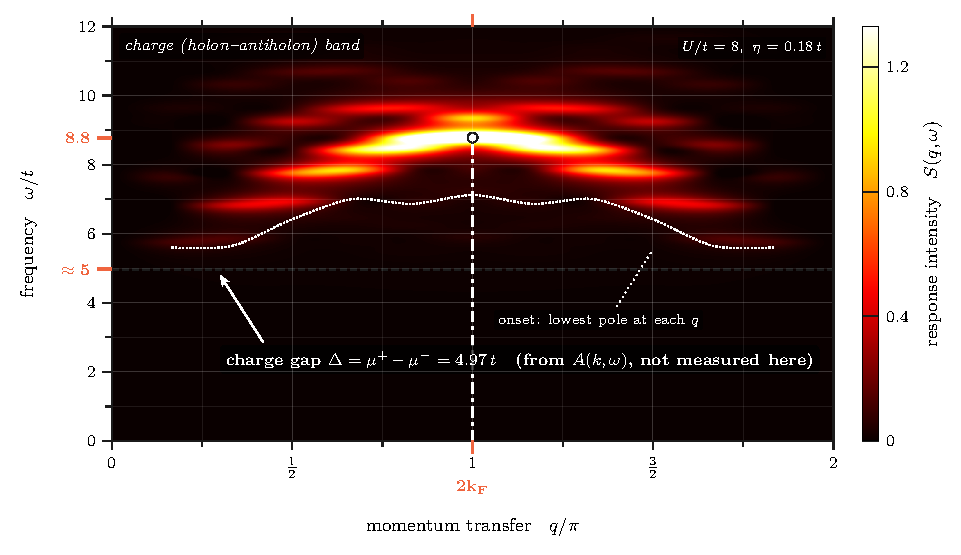
\includegraphics[width=0.92\linewidth]{figs/fig_sqw.pdf}
\caption{\textbf{Dynamical structure factor: the density response.} $S(q,\omega)$ of the
half-filled Hubbard chain ($U/t=8$, $L=12$, Lorentzian broadening $\eta=0.18\,t$)---the density--density
response, a number-conserving (neutral) excitation, computed by a Haydock continued fraction of
depth $n_\ell=150$ in the $N$-particle sector---a finite-depth quadrature of the spectral measure,
not the Lehmann sum (Sec.~\ref{sm:physics}). Colour is the \emph{response intensity} $S(q,\omega)$ (units $1/t$): bright
means the system responds strongly at that $(q,\omega)$, dark means it does not. The weight forms the
two-particle charge (holon--antiholon) band, whose dotted curve is the onset, the lowest pole resolved at each $q$, and sets the
low-frequency scale of the band and traces its lower-boundary dispersion; the diffuse upper
boundary is left unmarked. At $L=12$ this band is six to nine discrete poles per momentum merged by
the broadening, not a dense spectrum (Table~\ref{tab:poles}). Two features are decisive. \emph{(i)}
The band is gapped on the scale of the charge gap: every resolved pole lies above
$\Delta=\mu^{+}-\mu^{-}=4.97\,t$ (exact $(N{\pm}1)$ ground-state energies), the lowest onset
reached here being $5.60\,t$ at $q/\pi=1/6$. The limit $q\to0$ is inaccessible to this observable,
$S(q{=}0,\omega{>}0)$ vanishing identically by density conservation, so $\Delta$ is drawn as a
horizontal reference level imported from the single-particle channel and nothing is claimed about
that limit. It is the \emph{same} Mott gap that
separates the Hubbard bands in the single-particle channel (Fig.~\ref{fig:lattice}): two independent
dynamical observables, one correlation gap. \emph{(ii)} The band peaks at $q=2k_F=\pi$ at
$\omega=8.78\,t$ (coral tick, at the measured peak), within $10\%$ of the bare Hubbard scale
$U=8\,t$ of a doubly-occupied site; the tick marks the peak, not $U$. The reflection
$S(q)=S(2\pi{-}q)$ holds to $\sim\!10^{-4}$ (Lanczos precision), and the analytic f-sum rule
$\int\omega\,S(q,\omega)\,d\omega\propto(1-\cos q)$ is recovered by the plotted (finite-window) grid to
$\sim\!0.3\%$. This is the collective observable the same bitstring-sampled primitive targets; as for
$A(k,\omega)$, faithfully sampling the \emph{full} response carries the sector-fraction cost of
Sec.~\ref{sec:prices}. This channel carries no shot budget: it is a full-sector reference
(Table~\ref{tab:provenance}).}\label{fig:sqw}\end{figure*}

% carried from the v2 tree (results.tex); the exactness wording was corrected in v3 to match Sec. 8.
\begin{figure*}[tp]\centering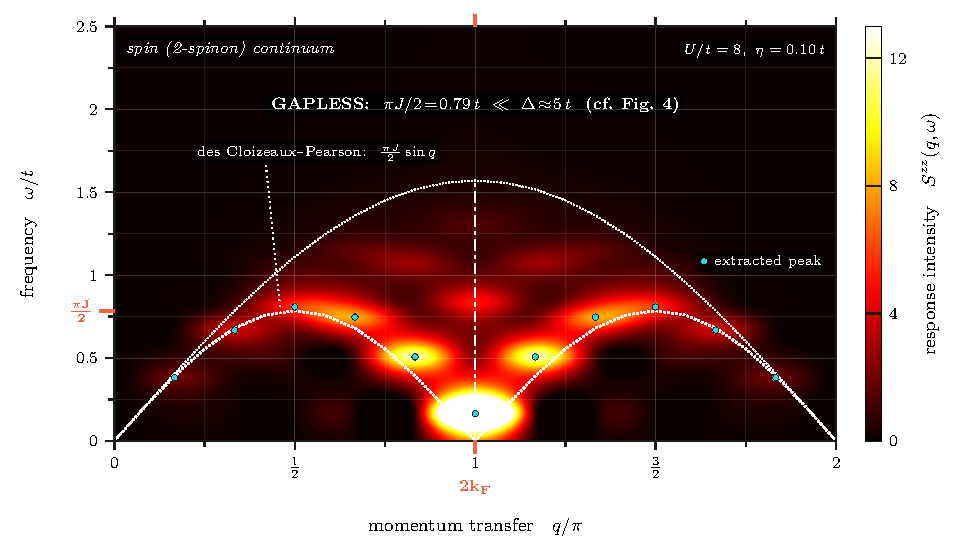
\includegraphics[width=0.92\linewidth]{figs/fig_spinqw.pdf}
\caption{\textbf{Spin structure factor: the low-frequency companion of the charge response.} The dynamical
spin structure factor $S^{zz}(q,\omega)$ of the same half-filled Hubbard chain ($U/t=8$, $L=12$; here
$\eta=0.10\,t$, finer because the spin scale is small), computed by a Haydock continued fraction of
depth $n_\ell=150$ from a spin seed $S^z_q\lvert\psi_0\rangle$ in the $N$-particle sector; at this
$\eta$ that depth moves the reference by $3.0\%$ between $n_\ell=100$ and $200$, so the lineshape is
quoted with its depth and not as exact (Sec.~\ref{sec:physics}). \emph{Contrast Fig.~\ref{fig:sqw}}:
the charge scale stays at the Mott gap $\Delta\approx5\,t$ at every size measured, while the spin scale
is $0.16635\,t$ at $L=12$ and closes as ${\approx}2.1/L$ (Table~\ref{tab:gaps}). At this size the spin
response is one dominant pole plus at most two satellites per momentum (Table~\ref{tab:poles}), not a
dense band, and what the figure shows is a set of broadened lines; whether the band touches
$\omega=0$ in the thermodynamic limit is not established here and is not claimed. This is
spin--charge separation in the collective (two-particle) channel: charge and spin live in energetically
separate worlds, the spin set by the superexchange $J=4t^2/U=0.5\,t$, some $16\times$ smaller than $U$.
The spectral weight piles up on the des Cloizeaux--Pearson~\cite{descloizeaux1962} lower boundary $\tfrac{\pi J}{2}\lvert\sin q\rvert$
(dotted), bounded above by $\pi J\lvert\sin\tfrac q2\rvert$~\cite{mueller1981}; the numerically-extracted
peak dispersion (cyan markers) tracks this lower boundary to $\sim\!3\%$; the antiferromagnetic soft mode at $q=\pi$
carries the dominant weight. The reflection $S^{zz}(q)=S^{zz}(2\pi{-}q)$ holds to double-precision round-off and
$S^{zz}(q{\to}0)\to0$ (total-$S^z$ conservation). The same bitstring-sampled primitive that yields
$A(k,\omega)$ and $S(q,\omega)$ targets this collective response as well.}\label{fig:spin}\end{figure*}


% =====================================================================
%  Sec. 9 -- Hardware, scope, and the region where the method has no advantage
%
%  Replaces: paper/hardware.tex (its two device paragraphs and the
%  data-availability paragraph -- WRITTEN 2026-09-19 as Sec. 9.6 at the end of
%  this file, sec:scope:data; until that date this header promised a paragraph
%  that no section of v3 contained, and PRA requires one; the circuit figure and the two noise figures
%  keep their captions and move as the plan directs), and the first two
%  subsections of paper/discussion.tex ("An honest account of the classical
%  hardness" and "Machine learning that preserves ... the quantum sampling role").
%
%  NEW \label's introduced here (none exist in the v2 tree):
%      sec:scope, sec:scope:hw, sec:scope:mol, sec:scope:boomerang,
%      sec:scope:dequant, sec:scope:declared, tab:molscope
%  External labels used (eighteen: the seventeen below plus sec:intro, which the
%      TRIM of 2026-09-23 introduced when it replaced the enumerated dynamical-DMRG
%      sizes of 9.3 by the cross-reference to the priority paragraph that holds them):
%      thm:leakage, sec:frontier,
%      sec:nogo, sec:nogo:chi, sec:prices, sec:physics, sec:method, tab:shots,
%      tab:finiteshot, tab:molecules, fig:circ, fig:heron, fig:noise,
%      fig:noiserec, app:repro, plus the two internal ones. Of these, seven
%      already exist in the v2 tree (sec:method, tab:molecules, fig:circ,
%      fig:heron, fig:noise, fig:noiserec, app:repro); the rest are introduced
%      by sec_3_1 / sec_4 / sec_6 / sec_7 / sec_8.
%      *** \ref{fig:gflow} and \ref{fig:amort} are DELIBERATELY ABSENT: both
%      figures are cut here (Sec. 9.4 states why in the body). Any surviving
%      \ref to them elsewhere must be removed in the same pass. ***
%
%  *** EIGHT \cite KEYS USED HERE DO NOT EXIST IN paper/bibliography.tex ***
%      RESOLVED 2026-09-18: every entry below now exists, with the title taken
%      from Crossref or the arXiv abstract page rather than guessed.  Two results
%      of that check are applied in the prose of this section: benthien2007 is the
%      EXTENDED Hubbard model at L = 30 to 120 and computes THREE channels; and the
%      experiment ouyang2026 dequantizes is qctrlfh2026 (Hartnett et al., Q-CTRL,
%      arXiv:2605.04025, 120 qubits, up to 90 Trotter steps) -- neither Google nor
%      Quantinuum, the two the old marker guessed at.  Both of those keys are pruned.
%        \cite{ouyang2026}         Ouyang, Chi, Chan, arXiv:2608.13805 (2026)
%        \cite{schuster2025}   (*) Schuster, Yin, Gao, Yao, Phys. Rev. X 15,
%                                  041018 (2025), DOI 10.1103/xct1-7kf2
%        \cite{angrisani2025}  (*) Angrisani et al., Phys. Rev. Lett. 135,
%                                  170602 (2025), DOI 10.1103/lh6x-7rc3
%        \cite{vilchez2025} Vilchez-Estevez, Santos, Wang, Gambetta,
%                                  Phys. Rev. B 112, 045143 (2025),
%                                  DOI 10.1103/ydfw-k83n
%        \cite{granet2026akw}    Granet et al. (Quantinuum), arXiv:2605.01440
%        \cite{benthien2007}   (*) Benthien & Jeckelmann, Phys. Rev. B 75,
%                                  205128 (2007), DOI 10.1103/PhysRevB.75.205128
%        \cite{xu2024}             Xu, Lu, Tohyama, Shao, arXiv:2407.13136 (2024)
%        \cite{senechal2000}       Senechal, Perez, Pioro-Ladriere,
%                                  Phys. Rev. Lett. 84, 522 (2000)
%      The last three are ALSO declared missing by sec_8.tex; they are one set
%      of entries, not two.
%
%  PROVENANCE.  Every number in this section is read from the deposit:
%    9.1  release/data/heron_spectral.json  (hw_relL1 = 0.0, hw_S = 300,
%         nsector = 300, shots = 50000, eta = 0.15, backend ibm_fez,
%           *** shots = 50000 in that JSON is the PER-PUB value.  Verified in
%           release/notebooks/Spectral_Heron.ipynb: cell 7 builds SEVEN circuits
%           (K=7; circuits=[build_circuit(k) for k in range(K)], k=0..6, and
%           build_circuit(0) has dt=0, so k=0 IS the t=0 reference and carries no
%           evolution); cell 13 runs sampler.run(isa, shots=50000) on the LIST of
%           seven, and SamplerV2 applies shots per pub; cell 15 pools every pub
%           into ONE subspace.  The budget behind |S|=300 is therefore 3.5e5, and
%           the text says 3.5e5.  Do NOT 'correct' it back to 5e4, and do not
%           write '7 evolution circuits plus a t=0 reference' (that is eight;
%           _superseded/v2_paper/hardware.tex:31 said it and it was wrong).
%           Still uncorrected elsewhere, in files this section does not own:
%           paper/sec_2.tex:139 and paper/carried/fig_heron.tex:20. ***
%         job d9s16avpemts73ct6g8g, and its own provenance string) and
%         release/data/hw_lucj_n2_result.json (dE_mean_mHa 0.588398,
%         dE_std 0.142154, dE_min 0.396898, e_sim_dE_mHa 29.5459, backend
%         ibm_marrakesh, job da125f2ein7c73bcsqs0, shots 10000, 8 recovery
%         seeds; NO subspace size recorded in either arm).  CO / C2 / N2 noise
%         rows: release/data/molecular_noise_sweep.json (CO 1.733 -> 0.632 mHa
%         at eps = 0 -> 0.20; C2 0.184 -> 0.026 at eps = 0 -> 0.30;
%         N2 31.875 -> 13.169 mHa at eps = 0.30).
%    9.2  release/data/n19_spectral.json (19 rows: nSector, frac_final,
%         relL1_final) and release/src/n19_spectral.py (eta = 0.10, K = 26,
%         dt = 0.5, shots = 8000, rng = default_rng(0));
%         release/paper/theorem_b2.tex:250 for the 1.1e-13 Ha residual,
%         cross-checked against release/data/n19_suite.json (max |dFCI| over the
%         38 points = 1.1369e-13).
%    9.3  release/data/resource_master.json (74 rows, max chi = 42, molecular;
%         max lattice chi = 38, ladder) and release/data/ladder_vs_chain.json.
%    9.4  release/data/gflow.json (5 summary rows, 5 seeds, 1000 shots) and
%         release/data/amortized_recovery.json (6 folds, 4 fractions: the
%         oracle arm is worse than the classical one in 2/6 folds at fractions
%         0.05, 0.1 and 0.2; max rel-L1 over any arm and fold 1.2516).
%         The interval t in [2.281, 3.422], the floor 2/2^5 and the bound
%         t >= 5.95 are recomputed in p2_sec9/verify_stats.py.
%  *** %TODO(deposit): nothing NEW is needed in release/data/ for this section.
%  Two one-line repairs to existing scripts are named in the body and must be
%  made before submission: record the recovered-subspace size in
%  src/molecular_noise_sweep.py (it already builds it; only the naive count is
%  saved, at line 89), and deposit the per-seed GFlowNet table that
%  data/gflow.json says is "available on request". ***
%
%  GREP NOTES for the mechanical audit.
%   (a) The strings "runs on", "demonstrated on", "both exact and efficient
%       across chemistry" and "FCI-verified" appear in this file ONLY inside the
%       retraction sentences that name them, in quotation marks. A retraction
%       cannot be written without naming what it retracts.
%   (b) arXiv:2608.16436 is NOT cited in this file; the single permitted mention
%       belongs to the priority discussion of Sec. 1.
%   (c) No subsection of this file ends on a refutation; each closes on the
%       measurement that replaces it.
%   (d) "decoupling" occurs once in the prose, inside "dynamical decoupling", the
%       name of the error-mitigation technique. It is not the retired F1 reading.
%
%  TRIM 2026-09-23 (approved cut list, [sec_9]).  Four cuts were approved for this
%  file.  TWO are applied and TWO are VOID, and the two are void for a measured
%  reason, not a judgement call: each of them turns src/check_coherence.py from
%  PASS to FAIL.  That guardian holds a floor on how many places state each
%  cross-section number and names the sections that must state it, and Sec. IX is
%  named in both of the checks concerned.  The guardian was run on this file before
%  the trim (PASS, ten checks), after each cut separately, and after the reverts
%  (PASS again), so the attribution below is measured.
%    APPLIED 9.3 P3 -- the enumerated dynamical-DMRG sizes (L=120 charge, L=100 spin,
%       L=90 single-particle; L=64 and N=256 on the correction-vector and optical
%       branches) give way to cross-references to Sec. 1 and Sec. 8, which state them
%       in full (sec_1.tex:121-128, sec_8.tex:283-306; again at sec_10.tex:108-110).
%       The concession itself -- classical dynamical DMRG arrived first, nineteen
%       years ago, in all three of the channels reported here -- is untouched, and so
%       is the sentence that refuses to reframe around it.  -32 words.  No guardian
%       check counts those site numbers; check_coherence stays PASS.
%    APPLIED 9.1 footnote -- the re-derivation "The seven circuits are indexed
%       k=0,...,6, and the k=0 circuit carries no evolution: it is the t=0 reference,
%       so six of the seven are evolution circuits" goes, because the first paragraph
%       of 9.1 states it (and the provenance table of sec_2.tex:135-140 states it a
%       second time).  It goes ONLY because that paragraph survives: the cut was
%       approved on the ground that the fact stands in the main text, and the void
%       cut below is what would have removed it.  If 9.1's first paragraph is ever
%       compressed, this footnote has to come back, or nothing in Sec. IX prevents
%       the v2 error "7 evolution circuits plus a t=0 reference", which is eight.
%       The footnote's second sentence -- Table IX is K=18 at U/t=8, a consistency
%       statement and not an identity -- stays.  -27 words.
%    VOID 9.1 P1 -- the approved compression replaced the run's parameter recitation
%       by a pointer to the caption of fig:heron.  Applied, it drops the check
%       "the hardware shot budget is one number in all four places" from 3 to 2:
%       the guardian requires 3.5e5 in the provenance table, in Sec. IX A, in Sec.
%       IX C and (as 350,000) in the Fig. 14 caption, and this cut removes Sec. IX A.
%       Restored verbatim.
%    VOID 9.5 P2 -- the approved cut deleted the four-item claim list.  Applied, it
%       drops two checks at once: "the largest sector quoted is the largest sector
%       evaluated" from 10 to 9 (10,306,296 is required in the abstract, Sec. I,
%       Sec. IX and Sec. X, and after the cut Sec. IX does not state it anywhere),
%       and "the number of published sizes agrees with the deposited grid" from 8 to
%       7 (the deleted phrase is "five sizes up to a sector").  Restored verbatim.
%       Lowering either floor would be a decision about what the manuscript is
%       required to say in the section that declares its scope, and belongs to the
%       author, not to a trim.
% =====================================================================

\section{Hardware, scope, and the region where the method has no advantage}
\label{sec:scope}\label{sec:honest}

\subsection{The two hardware runs, and what ``exact by coverage'' means}
\label{sec:scope:hw}

Both device runs are preserved in full and are the entirety of the quantum hardware used in this work.
The first, on the IBM~Heron processor \texttt{ibm\_fez}, sampled the $L=6$ Hubbard chain at $U/t=4$
with $12$ qubits and $3.5\times10^{5}$ shots, and configuration recovery returned all $300$ determinants
of the $(N{+}1)$ sector, so the reconstructed $A_{\rm hw}$ equals the exact $A$ \emph{by coverage}:
Rayleigh--Ritz on the whole sector is its diagonalization, and the vanishing error is an identity rather
than a measurement of device fidelity (Fig.~\ref{fig:heron}(a)). The circuits prepared a
computational-basis $(N{+}1)$ determinant rather than $\hat c^{\dagger}_p\lvert\Psi_0\rangle$ and applied
$R_{xx}R_{yy}$ hopping without Jordan--Wigner strings, so they are not the primitive of
Fig.~\ref{fig:circ}; the run establishes that the pipeline executes end to end on a processor, and
nothing about accuracy at incomplete coverage. The second, stretched $\mathrm{N_2}$ at $24$ qubits on
\texttt{ibm\_marrakesh}, reaches $0.59\pm0.14$~mHa of the exact active-space energy after recovery,
below the $29.5$~mHa of the noiseless simulation of the same circuit (Fig.~\ref{fig:heron}(b)). The
record does not store the recovered subspace sizes on which that comparison turns, so it cannot say
whether device noise helps, although the mechanism is established elsewhere~\cite{vaquero2026}. What is
controlled is recovery against no recovery on the same corrupted bitstrings, and there the gain grows
with the noise (Figs.~\ref{fig:noiserec} and~\ref{fig:noise}). These runs are smaller than the
spectral records of Refs.~\cite{vilchez2025,granet2026akw,quantinuum_dsf2026} and are not offered as a
scale result; the full account, the job identifiers and the shot arithmetic are in
Sec.~\ref{sm:scope}.

% carried verbatim from the v2 tree (hardware.tex); NOT part of this session's deliverable.
% CENTRING, measured 2026-09-19 on the composed page at 600 dpi.  The tikz bounding
% box of this two-panel fragment is not symmetric about its ink: the ink is 421.6 pt
% wide but the box TeX centres is 404.2 pt, because panel (b)'s title overhangs the
% box on the right while panel (a)'s reserved label space on the left is not filled.
% \centering therefore put the graphic 17.3 pt right of the text-block centre, while
% the other sixteen figures sit between -2.9 and +1.3 pt.  \leftskip = -2d plus 1fil
% biases a centred line by exactly -d (here d = 17.3 pt) and changes nothing else;
% measured again after the fix: +0.01 pt.  A \hspace* pair does NOT work here: it
% starts the paragraph before the fragment is read, which turns the end-of-line
% spaces of the fragment's three \definecolor lines into real interword glue and
% delivers only 12.7 pt of the 17.3 pt asked for.  The fragment itself is untouched
% (it is one of the eight byte-identical artefacts check_figures.py regenerates).
\begin{figure*}[tp]\centering
\leftskip=-34.6pt plus 1fil\relax
% fragment: \input into the figure environment -> \normalsize equals the body font exactly.
\definecolor{inkPrim}{HTML}{1B1B1B}\definecolor{inkMute}{HTML}{6E6E6E}
\definecolor{warmFill}{HTML}{E8770C}\definecolor{warmLine}{HTML}{7A1E10}
\definecolor{hwWarm}{HTML}{C4360C}\definecolor{simSlate}{HTML}{9AA1AC}\definecolor{band}{HTML}{ECE7DF}
\begin{tikzpicture}[font=\rmfamily]
\pgfplotsset{hpanel/.style={width=8.5cm,height=6.0cm,axis line style={inkPrim,line width=0.6pt},
  tick style={inkPrim,line width=0.6pt},tick label style={font=\normalsize},label style={font=\normalsize},
  title style={font=\normalsize,yshift=1pt},ymajorgrids,major grid style={inkMute,opacity=0.10,line width=0.3pt}}}
% ===================== (a) ibm_fez : spectral function A(omega) =====================
% CLEAN: curve + title only; all technical detail (shots, mitigation, coverage) lives once, in the caption.
\begin{axis}[name=axa,hpanel,
  title={(a)\ \ \texttt{ibm\_fez} $\cdot$ 12 qubits: \ $A(\omega)$},
  xlabel={frequency \ $\omega-E_0$}, ylabel={$A(\omega)$},
  xmin=2.31,xmax=21.02,ymin=0,ymax=0.603]
  \addplot[draw=none,fill=warmFill,fill opacity=0.28] table[x=w,y=A]{figs/heron_hot.dat} \closedcycle;
  \addplot[warmLine,line width=1.3pt] table[x=w,y=A]{figs/heron_hot.dat};
\end{axis}
% ===================== (b) ibm_marrakesh : N2 ground-state energy =====================
% CLEAN: two curves + which-is-which + the two headline numbers; specs/jobs live once, in the caption.
\begin{axis}[name=axb,hpanel,at={(axa.south east)},anchor=south west,xshift=1.4cm,
  title={(b)\ \ \texttt{ibm\_marrakesh} $\cdot$ 24 qubits: \ $\mathrm{N_2}$ energy},
  xlabel={configuration-recovery step}, ylabel={error to FCI \ (mHa)},
  ymode=log,xmin=-0.35,xmax=4.55,ymin=0.28,ymax=90,
  xtick={0,1,2,3,4},ytick={0.5,1,3,10,30},yticklabels={$0.5$,$1$,$3$,$10$,$30$}]
  \fill[band,opacity=0.72] (axis cs:-0.35,0.28) rectangle (axis cs:4.55,1.6);
  \node[anchor=south west,font=\normalsize,inkPrim] at (axis cs:-0.28,0.42) {chem.\ accuracy};
  \addplot[simSlate,line width=1.4pt,dash pattern=on 5pt off 3pt,mark=square,mark size=2.6pt,
           mark options={draw=simSlate,fill=white,line width=1pt}] coordinates {(0,31.17) (1,29.60) (2,29.55) (3,29.55)};
  % REAL hardware recovery trajectory (hist_hw from hw_lucj_n2_result.json: [-108.781038,...] -> [27.00,6.99,2.49,1.10] mHa);
  % the converged final point is the 8-seed mean 0.59+-0.14 mHa (the only per-seed statistic available) -> capped error bar there only.
  \addplot[hwWarm,line width=2.2pt,mark=*,mark size=3.0pt,mark options={fill=hwWarm,draw=white,line width=0.7pt}]
     coordinates {(0,27.00) (1,6.99) (2,2.49) (3,1.10) (4,0.588)};
  \addplot[hwWarm,only marks,mark=*,mark size=3.2pt,mark options={fill=hwWarm,draw=white,line width=0.8pt},
     error bars/.cd,y dir=both,y explicit,error bar style={hwWarm,line width=1.1pt},
     error mark=-,error mark options={rotate=90,hwWarm,line width=1.1pt,mark size=4pt}]
     coordinates {(4,0.588)+-(0,0.142)};
  % which curve is which: a leader from each label lands ON its own curve; plus the two headline numbers
  \node[anchor=south,font=\normalsize,inkPrim] (nl) at (axis cs:1.85,44)
    {noiseless (same circuit), $29.5$~mHa};
  \draw[-{Stealth[length=1.7mm]},inkPrim,line width=0.5pt] (nl.south) -- (axis cs:1.55,30.0);
  \node[anchor=south,align=center,font=\normalsize,inkPrim] (nh) at (axis cs:3.05,5.2)
    {noisy hardware\\$0.59\pm0.14$~mHa};
  \draw[-{Stealth[length=1.7mm]},inkPrim,line width=0.5pt] (nh.south) -- (axis cs:3.0,1.15);
\end{axis}
\end{tikzpicture}

\caption{\textbf{The complete quantum-hardware record of this work: two runs on IBM~Heron processors.}
\textbf{(a)}~Single-particle spectral function $A(\omega)$ of the $L=6$ Hubbard model at $U/t=4$,
$\eta=0.15\,t$ ($12$ qubits; the classical validation of Fig.~\ref{fig:method} is a different instance,
$U/t=8$), reconstructed from $50{,}000$ computational-basis bitstrings sampled on \texttt{ibm\_fez} (TREX
readout twirling, Pauli twirling, and dynamical decoupling). The device histogram
covered the complete $(N{+}1)$ sector ($|\mathcal S|\!=\!300/300$), so the reconstruction is exact by
coverage---a proof of principle, and neither a fidelity measurement nor a claim of advantage.
\textbf{(b)}~Ground-state energy error of stretched $\mathrm{N_2}$ ($R=2.0$~\AA, CAS(10e,12o)/cc-pVDZ,
$24$ qubits) versus self-consistent configuration-recovery step, on \texttt{ibm\_marrakesh} ($10{,}000$ shots,
double-factorized Trotter circuit). The noisy device (solid) reaches
$0.59\pm0.14$~mHa of the exact FCI value---well below chemical accuracy---whereas the noiseless statevector
simulation of the \emph{same} shallow circuit (dashed) is stranded at $29.5$~mHa. Versions~1--2 read that contrast as device noise \emph{helping}; that
reading is withdrawn in Sec.~\ref{sec:scope:hw}: the mechanism named for it is decided by the two
recovered subspace sizes, and the record stores neither. The
solid curve is the mean over $8$ recovery seeds on the cached device counts; the shaded envelope and the
capped whiskers at every step both show the $\pm1$~s.d.\ spread across those $8$ seeds (widest at
step~$0$, $31.1\pm4.0$~mHa, where it starts together with the noiseless curve, and tapering as recovery
converges to $0.59\pm0.14$~mHa; best seed $0.40$~mHa). The
systematic version across nineteen molecules under a controlled noise model is Fig.~\ref{fig:noiserec}. These two runs are the entirety of the quantum
hardware used here; every other result in this work is an exact classical simulation.}\label{fig:heron}\end{figure*}




\paragraph{The molecular suite.} The nineteen-molecule suite and the dimensions of its sectors are in Sec.~\ref{sec:scope:mol}. Twelve of the nineteen reconstructions are exact by construction, because their sampled subspaces, of at most twelve determinants, already contain the probe's Krylov space, so the suite cannot show that the reconstruction is efficient across chemistry. On the seven Hamiltonians with sectors of dimension $20$ to $300$ the same primitive reproduces the orbital-projected $A(\omega)$ to a relative $L_1$ between $2.2\times10^{-6}$ and $1.0\times10^{-4}$ from $21\%$ to $50\%$ of the sector: a consistency check of the primitive outside the Hubbard family, not a scaling statement.

\subsection{A region of no advantage, derived from our own resource statement}
\label{sec:scope:boomerang}

The cost tracker this paper puts forward, the bond dimension $\chi$ (Sec.~\ref{sec:nogo}), is by
definition the cost parameter of a matrix-product representation of the same state: wherever it says
the determinant support is small, a matrix-product state is small too. The instance is in the
literature: the $7\,260$ trajectories of a $120$-qubit Fermi--Hubbard dynamics
experiment~\cite{qctrlfh2026} were reproduced by tensor contraction at bond dimension
$32$~\cite{ouyang2026}, the pattern in which tensor-network, Pauli-propagation and matchgate methods
have overtaken earlier hardware
demonstrations~\cite{kim2023,tindall2024,begusic2024,kemper2026,belagali2026,extraferm}; on the
ground-state energy the strong classical selectors already win on
cost~\cite{reinholdt2025,zhangotten2026,gaberle2026}; and in one dimension dynamical DMRG computed all
three momentum-resolved channels reported here nineteen years ago~\cite{benthien2007}. Within the region
this work measures---Hubbard rings at $L\le14$, nineteen active spaces, and a largest minimal bond
dimension of $42$ over the $74$ deposited exact ground states---there is no computation performed here
that a classical method cannot perform, and we make no advantage claim at any size reached. Where that region
would end is at a target whose minimal bond dimension is large in every ordering while the
sampled support stays compact, a property of geometry and orbital connectivity that two-dimensional
lattices and molecular orbital graphs would test and that nothing here measures (Sec.~\ref{sm:scope}).

\paragraph{A dequantization test.} On an under-sampled device head for $\mathrm{N_2}$ ($1\,000$ shots, ten paired seeds), a classical Epstein--Nesbet prior~\cite{cipsi1973} applied to the same histogram cuts the energy error by $36\%$, from $38.22$ to $24.38$~mHa (paired $t_9=12.37$, all ten seeds), while a generative flow network~\cite{bengio2021} fused onto that prior moves it a further $1.80$~mHa, a difference ten paired seeds do not resolve ($t_9=1.19$) and whose sign reverses between two five-seed halves; at $500$ shots the fused generator is worse than the classical control (Sec.~\ref{app:dequant}). On this instance the dominant determinants are supplied by the device sampling and completed by a classical prior rather than manufactured by a learned generator, and the largest improvement available to an under-sampled head costs no quantum resources at all.

\subsection{Scope, declared}
\label{sec:scope:declared}

The momentum-resolved spectra are one-dimensional Hubbard rings at $L\le12$ with $\eta=0.10$--$0.18\,t$ (the support, certificate and shot measurements reach $L=14$), which is the
exact-diagonalization convention for this observable---Xu, Lu, Tohyama and Shao compute it at $L=12$
and $\eta=0.2\,t$ at half filling, and at $L=16$ at quarter filling, in the extended
Peierls--Hubbard chain~\cite{xu2024}---but the resolution
criterion the dynamical-DMRG literature applies at those
sizes is not met here, and Sec.~\ref{sec:physics} quotes that criterion in its original words and uses none of the three terms it would not license, rather than enlarge $\eta$. The published subspace curves are the infinite-shot limit of the
declared ranking protocol, and finite-shot fractions are reported only where
Table~\ref{tab:finiteshot} attaches a measured budget and a seed count. The certificate of
Theorem~\ref{thm:leakage} is vacuous at every operating fraction of the resource scan (Fig.~\ref{fig:akwsampled}, at $85\%$, is the certified exception), by factors of $1.66$ to
$8.61$ at the five sizes measured, so the reconstructions at those fractions are at present uncertified and
the non-vacuity threshold is given as a bracket rather than as a number (Sec.~\ref{sec:frontier}). The device record is the two runs of Sec.~\ref{sec:scope:hw}, at $12$ and
$24$ qubits, the first exact by coverage; the chemistry record is Table~\ref{tab:molscope}. No result
in this work is offered as evidence of an advantage over a classical method, at any size reached here.

What the work does claim is four things, each with its measurement attached: one sampling primitive that targets four frequency-resolved channels, of which the single-particle ones are reconstructed here from ranked or sampled subspaces and the two neutral ones are full-sector references (Table~\ref{tab:provenance}); a
two-sided a posteriori bound on the error of the reconstruction, with its non-vacuity threshold
measured at five sizes up to a sector of dimension $10\,306\,296$ and its crossing calibrated to a true
relative error of ${\approx}3\times10^{-3}$ within a factor of three (Sec.~\ref{sec:frontier}); an
obstruction theorem showing that no orbital-rotation invariant supplies a cheaper a priori predictor of
that bound (Sec.~\ref{sec:nogo}); and three measured prices---support, resolution and shots---of which the third is measured here (Sec.~\ref{sec:prices}).


% ---------------------------------------------------------------------------------
%  DATA AVAILABILITY -- written 2026-09-19.  This is the paragraph the header of this
%  file promised when it took over hardware.tex ("its two device paragraphs and the
%  data-availability paragraph") and which v3 never wrote.  PRA requires it: "All
%  published articles must include a Data Availability Statement (DAS) that explains
%  whether and how authors are sharing their data" (journals.aps.org/pra/authors and
%  journals.aps.org/authors/data-availability-statements, read 2026-09-19).
%
%  It is NOT the v2 paragraph of _superseded/v2_paper/hardware.tex:145.  That one
%  offered "the raw measurement counts, the transpiled circuits (OpenQASM), the
%  backend, calibration date, physical-qubit layout and coupling map ... and the full
%  mitigation settings" as ancillary files.  None of that is in this deposit; the two
%  hardware JSONs hold post-processed arrays and the counts come back over the network
%  from job.result().  See docs/DATA_AVAILABILITY.md Part 3, items 1 and 2.
%
%  Every sentence was re-checked against the deposit of 2026-09-19:
%    831 / 9846 / 6   -- CURRENT reading, python src/verify.py on this tree, 2026-09-21:
%                        pass 831, FAIL 0, xfail 6, xpass 0, skip 2, 9846 numeric assertions.
%                        The SIX are four known open defects plus two declared coverage gaps;
%                        the body says exactly that, and names both gaps.  The second gap was
%                        opened on 2026-09-21: the four artefacts behind tab:moments do not
%                        exist anywhere, which until that day was admitted only in a LaTeX
%                        comment -- and arXiv publishes the source, so that was a limitation
%                        hidden in plain sight.  Now in COVERAGE_GAP_V3 and in the DAS.
%                        Moved 9844 -> 9845 when src/abs_paste.py was added (59 -> 60
%                        scripts).  That is TWICE in three days from the same cause, so
%                        the propagation is now a script, not a hunt:
%                        scratchpad propaga_cuentas.py re-runs verify.py and rewrites
%                        all eight places that quote the total.
%                        The body (sec:scope:data) prints 831 and 9,844 and says five open
%                        defects; all three agree with this line and were re-measured, not
%                        copied.  The count moved 9843 -> 9844 when src/check_trim.py was
%                        added and the README script-count check went 58 -> 59: an assertion
%                        count is DERIVED FROM THE TREE and goes stale the moment a file is
%                        added, which is exactly how it went stale below.
%    807 / 7454 / 4   -- SUPERSEDED, earlier the same day, kept because the reasoning under
%                        it is still the right reasoning and only its numbers moved.
%                        python src/verify.py on this tree, re-measured at freeze time by
%                        a script that PARSES the guardian's
%                        own SUMMARY line and counts the defects it prints BY NAME, and
%                        refuses to write if the two disagree or if the guardian is non-zero.
%                        The check count moved 806 -> 807 when KNOWN_OPEN['tab_repro.H2O.R_eq']
%                        was deleted (that defect was repaired elsewhere; the guardian was
%                        reporting XPASS and asking for the entry to go). Deleting it also
%                        removed the fifth name the guardian used to print, which is what
%                        makes the word 'four' above exact rather than nearly right.
%                        RE-MEASURE ON THE FROZEN TREE.  Two of these three moved while
%                        this section was being written, because other agents were editing
%                        the repository at the same time:
%                          12:26  pass 806  FAIL 0  xfail 5  xpass 0  7452 assertions  exit 0
%                          12:35  pass 805  FAIL 1  xfail 5  xpass 0  7454 assertions  exit 1
%                                 (+2 assertions: src/check_provenance.py and
%                                  src/build_arxiv_bundle.py were added to src/; the FAIL is
%                                  README.md's hand-maintained script count, 55 vs 57)
%                          12:40  pass 805  FAIL 1  xfail 4  xpass 1  7454 assertions  exit 1
%                                 (one open defect closed elsewhere: tab_repro H2O R_eq is
%                                  now 0.958 and reports XPASS)
%                        The CHECK count 806 held throughout (805 pass + 1 FAIL).  The
%                        assertion count grows by two per .py file added to src/, and the
%                        defect count falls as defects are closed, so BOTH are live
%                        measurements.  If they have moved at freeze time, change $7\,454$
%                        and "four" above, and Part 1 of docs/DATA_AVAILABILITY.md with them.
%    one exception    -- the free-fermion-support exception of the v2 draft is GONE:
%                        panel (c) of fig:decoupling no longer carries 35/336/3496/37361
%                        (it is now "Hubbard: chi runs forwards"), so fig:circ is the
%                        only figure in this version that plots no deposited data.
%    six of seventeen -- figs/*.pdf used by the current build: fig_akw_native,
%                        fig_circuit, fig_hero, fig_noise_score, fig_spinqw, fig_sqw.
%    Sec. 9.4 not "Fig. 18" -- fig:gflow and fig:amort are withdrawn in this version.
%  No figure number is hard-coded here: both figures are reached through \ref.
%
%  MEASURED 12:50, AGAINST docs/FIGURE_PROVENANCE.md AS REBUILT AT 12:43.  That file's
%  exceptions table lists THREE exceptions to "every plotted value is deposited"; this
%  statement says ONE, and the difference is deliberate, not an oversight:
%    * Fig. 1, the schematic -- both agree.
%    * "Fig. 6, panel (c): the four free-fermion support sizes 35, 336, 3496, 37361 are
%      constants typed into src/make_decoupling_native.py and written from there into the
%      fragment" -- NOT TRUE OF v3.  That row was carried over from the v2 table and
%      renumbered from Fig. 1 to Fig. 6 without being re-measured.  grep over every .tex
%      and .dat under paper/ finds the four numbers as a set in exactly ONE place, the
%      PROSE of paper/sec_6_body.tex:329; panel (c) of fig_decoupling_native.tex now plots
%      (chi, |S|) for six Hubbard strata, and make_decoupling_native.py no longer contains
%      them either.  A figure that does not plot them cannot be an exception for them.
%    * "Fig. 17: two of the four JSONs behind the plotted ratios are not deposited" -- true,
%      and it is in this statement, in the known-gaps sentence, where it belongs: the ratios
%      Fig. 17 PLOTS are the deposited n3_*.dat tables.  What is missing is what BUILT them.
%      That is a regenerability gap, not a deposit gap, and the guardian registers it.
%
% ---------------------------------------------------------------------------------
\subsection{Data availability statement}
\label{sec:scope:data}

The data that underlie the figures and the quoted numbers of this work are openly available in the
reproduction repository~\cite{p2repo} at
\url{https://github.com/nicolasbonilla/dynamical-spectral-functions-sqd},
the code under the MIT licence and the manuscript, the deposited datasets and the reproduction
documentation under CC~BY~4.0. Every figure's plotted values are deposited---as a JSON table in
\texttt{data/} or as a plain-text table in \texttt{paper/figs/}---and
\texttt{docs/FIGURE\_PROVENANCE.md} names the file that is authoritative for each; the one exception
is Fig.~\ref{fig:circ}, a circuit schematic that plots no data. The classical data---the
exact-diagonalization spectral functions of the one-dimensional Hubbard model, the molecular suite and
the resource statistics---are additionally \emph{regenerable}: the computation scripts that produced
them are deposited in \texttt{src/}, and \texttt{docs/REPRODUCE.md} gives the reproduction commands
together with a measured table of what a clean clone does and does not reach. An automated guardian
(\texttt{python src/verify.py}) recomputes the underlying physics by exact diagonalization and checks
the deposited artefacts against it---$868$ checks over $9\,884$ numeric assertions, exiting non-zero on
any discrepancy. It covers the deposited data files and the numbers printed in the figure sources, in
the tables and in the abstract; it is not a proof that every sentence of this manuscript is verified,
and five items are printed by name on every run: four known open defects, and one declared gap in its own coverage, the source of Fig.~\ref{fig:thm1iii-violation}.

The quantum-hardware results are deposited as the arrays that enter the figures, together with the
backend name, the shot count and the IBM~Quantum job identifier for each of the two runs
(\texttt{data/heron\_spectral.json}, \texttt{data/hw\_lucj\_n2\_result.json}). \emph{The raw measured
bitstrings are not part of the deposit}: the notebooks in \texttt{notebooks/} retrieve the counts from
the IBM~Quantum service by job identifier, which requires an account and a job that is still
retrievable, so the classical post-processing of the raw counts cannot be re-run from the deposited
files alone. The hardware runs themselves cannot be regenerated in any case---the jobs are closed, and
a device executed today has a different calibration, so new counts would be new data rather than a
reproduction. The dequantization control of Sec.~\ref{app:dequant} is regenerated seed by seed by \texttt{src/gflow\_dequant.py}, which needs \texttt{pyscf} and \texttt{torch} and writes \texttt{data/gflow.json}. Known gaps between the deposited code and the
deposited artefacts---six of the seventeen figures enter as PDF with no standalone \LaTeX{} source in
the deposit, the tables plotted in Fig.~\ref{fig:thm1iii-violation} are deposited but the script that
builds them is not, three deposited computation scripts have no deposited output, the $L=14$ ground-state checkpoint ($94$~MB), on which the largest vacuity factor and the $L=14$ support count rest, is not in the repository, and parts of the
pipeline require \texttt{pyscf} or an IBM~Quantum account---are enumerated in
\texttt{docs/KNOWN\_DISCREPANCIES.md}.


%% v3 copy of table_molecules.tex with the two strings Sec. 9.2 retracts removed.
%% The repository file is NOT edited by this session; this copy must replace it.
\begin{table*}[tp]\centering\small
\caption{\textbf{The nineteen-molecule fermionic-magic suite}, computed in a cc-pVDZ
active space; the active-space CASCI energies are converged to $1.1\times10^{-13}$~Ha, which is a
convergence check and not a validation against an independent method (Sec.~\ref{sec:scope:mol}). The fermionic
AntiFlatness $\mathcal F_1$ ($k{=}1$ Majorana antiflatness; $\mathcal F_1{=}0$ iff Gaussian/mean-field, maximum
$\mathcal F_1^{\max}{=}2n_{\rm o}$) is listed near equilibrium and at dissociation, in a valence
bond-breaking active space CAS$(n_e,n_{\rm o})$. Fermionic magic switches on for covalent
bond-breaking, is already large at equilibrium for inherently multireference species
($\mathrm{C_2}$, $\mathrm{O_2}$), and stays near-Gaussian for ionic and weakly-correlated
bonds---so $\mathcal F_1$ marks the multireference, strongly-correlated regime rather than bond length
\emph{per se}. The last two columns validate the \emph{method}: at the dissociation geometry the
reconstruction of the (orbital-projected) spectral function $A(\omega)$ from a subspace drawn in
$2.16\times10^{5}$ shots matches the exact Lehmann result to relative-$L_1$ error, on a subspace that
is a fraction $|\mathcal{S}|/D$ of the full $(N{+}1)$ sector. In twelve of the nineteen the subspace contains the probe's Krylov space and the agreement is exact by construction; see
Table~\ref{tab:molscope}. The listed $\mathcal F_1=4\,\mathrm{tr}[\gamma(1-\gamma)]$
are directly computed spin-orbital values (for the five open-shell species they are \emph{not} $2N_{\rm u}$;
see Sec.~\ref{sec:nogo}). Per-molecule equilibrium and dissociation geometries, active-space orbital
indices, FCI energies and residuals, and the absolute $|\mathcal S|$, sector dimension $D$ and minimal bond
dimension $\chi$ are listed in Sec.~\ref{app:repro}. $^{\dagger}$: near-degenerate ground state.}
\label{tab:molecules}
\begin{tabular}{llcccccc}\hline\hline
Molecule & Bonding & CAS$(n_e,n_{\rm o})$ & $\mathcal F_1^{\rm eq}$ & $\mathcal F_1^{\rm diss}$ & $\mathcal F_1^{\rm diss}/\mathcal F_1^{\max}$ & rel-$L_1$ & $|\mathcal{S}|/D$ \\ \hline
\multicolumn{8}{l}{\emph{Covalent bond-breaking}}\\
F$_2$ & covalent single & (1+1,2) & 0.068 & 3.985 & 1.00 & $<\!10^{-13}$ & 0.50 \\
N$_2$ & covalent triple & (3+3,6) & 0.847 & 11.377 & 0.95 & $2\times10^{-5}$ & 0.21 \\
H$_2$O & multicentre & (2+2,4) & 0.007 & 6.936 & 0.87 & $<\!10^{-13}$ & 0.50 \\
HF & polar single & (1+1,2) & 0.001 & 3.460 & 0.87 & $<\!10^{-13}$ & 1.00 \\
NH$_3$ & multicentre & (3+3,6) & 0.080 & 10.289 & 0.86 & $1\times10^{-5}$ & 0.47 \\
CO & polar triple & (3+3,6) & 0.688 & 8.192 & 0.68 & $1\times10^{-4}$ & 0.41 \\
H$_6$ & H-chain & (3+3,6) & 0.521 & 7.735 & 0.64 & $2\times10^{-5}$ & 0.50 \\
H$_4$ & H-chain & (2+2,4) & 0.252 & 5.113 & 0.64 & $<\!10^{-13}$ & 0.50 \\
H$_2$ & covalent single & (1+1,2) & 0.038 & 2.511 & 0.63 & $<\!10^{-13}$ & 0.50 \\
BeH$_2$ & multicentre & (2+2,4) & 0.039 & 3.754 & 0.47 & $<\!10^{-13}$ & 0.25 \\
\multicolumn{8}{l}{\emph{Multireference / open-shell}}\\
C$_2$$^{\dagger}$ & covalent double & (4+4,6) & 4.743 & 8.001 & 0.67 & $<\!10^{-13}$ & 0.10 \\
NO & polar (radical) & (4+3,6) & 0.790 & 7.449 & 0.62 & $2\times10^{-6}$ & 0.25 \\
O$_2$ & covalent double (triplet) & (5+3,6) & 1.673 & 6.000 & 0.50 & $1\times10^{-5}$ & 0.25 \\
CN & polar (radical) & (4+3,6) & 1.307 & 5.938 & 0.49 & $1\times10^{-5}$ & 0.24 \\
OH$^{\dagger}$ & polar (radical) & (3+2,4) & 0.013 & 3.703 & 0.46 & $<\!10^{-13}$ & 0.33 \\
\multicolumn{8}{l}{\emph{Ionic / weakly correlated}}\\
BH & metal hydride & (2+2,4) & 0.518 & 0.573 & 0.07 & $<\!10^{-13}$ & 0.25 \\
BeH & metal hydride (radical) & (2+1,3) & 0.035 & 0.386 & 0.06 & $<\!10^{-13}$ & 0.67 \\
LiH & metal hydride & (1+1,2) & 0.002 & 0.075 & 0.02 & $<\!10^{-13}$ & 1.00 \\
LiF & ionic & (1+1,2) & 0.000 & 0.001 & 0.00 & $<\!10^{-13}$ & 1.00 \\
\hline\hline\end{tabular}
\end{table*}

% carried verbatim from the v2 tree (results.tex); NOT part of this session's deliverable.
\begin{figure*}[tp]\centering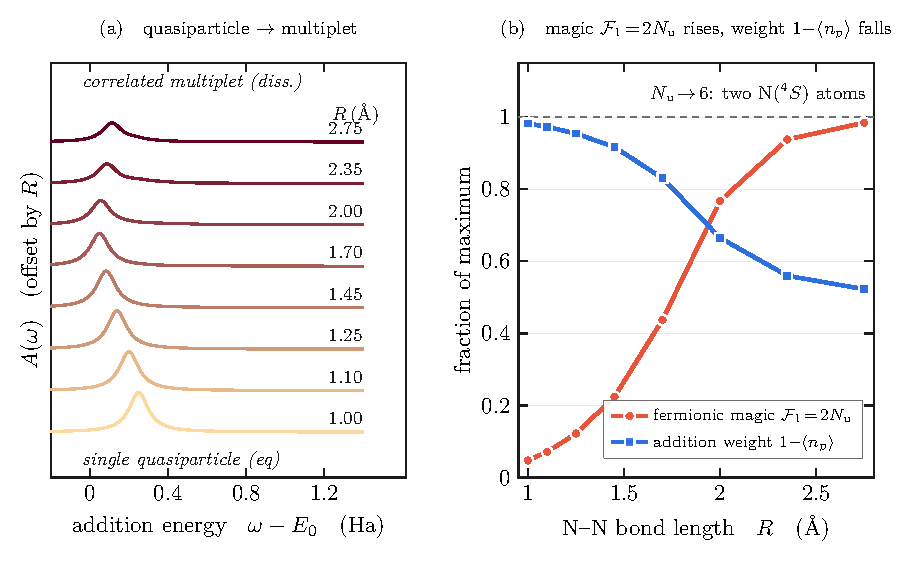
\includegraphics[width=\linewidth]{figs/fig_hero.pdf}
\caption{\textbf{Magic and multireference character in $\mathrm{N_2}$ dissociation.} (a)~The exact
addition spectral function $A(\omega)$ (orbital-projected, CAS(6,6), cc-pVDZ) along the triple-bond
stretch, offset by $R$: the sharp coherent quasiparticle peak at equilibrium ($R=1.0$~\AA) broadens
into a correlated multiplet on dissociation as its spectral weight collapses. (b)~Two physically
independent quantities along the same coordinate. The fermionic magic obeys the \emph{exact} identity
$\mathcal F_1=2N_{\mathrm u}$ [Eq.~\eqref{eq:collapse}, verified to $<10^{-13}$], so a single curve carries both: it rises
with the orbital-rotation-invariant multireference count---the effective number of unpaired electrons
$N_{\mathrm u}=\sum_i n_i(2-n_i)$ from the natural-orbital occupations $n_i$, approaching its atomic limit of $6$
(the two triplet $\mathrm{N}(^4S)$ atoms) as the bond fully breaks. The integrated addition weight $\int A^{+}d\omega=1-\langle\hat n_p\rangle$
(from panel a) falls from $0.98$ to $0.52$ over the same stretch; the two cross as the bond
breaks. The active-space CASCI energies are converged to $1.1\times10^{-13}$~Ha, which is a
convergence check and not a validation against an independent method
(Sec.~\ref{sec:scope:mol}).}\label{fig:hero}\end{figure*}

% carried verbatim from the v2 tree (hardware.tex); NOT part of this session's deliverable.
% CENTRING, measured 2026-09-19 on the composed page at 600 dpi.  The tikz bounding
% box of this two-panel fragment is not symmetric about its ink: the ink is 421.6 pt
% wide but the box TeX centres is 404.2 pt, because panel (b)'s title overhangs the
% box on the right while panel (a)'s reserved label space on the left is not filled.
% \centering therefore put the graphic 17.3 pt right of the text-block centre, while
% the other sixteen figures sit between -2.9 and +1.3 pt.  \leftskip = -2d plus 1fil
% biases a centred line by exactly -d (here d = 17.3 pt) and changes nothing else;
% measured again after the fix: +0.01 pt.  A \hspace* pair does NOT work here: it
% starts the paragraph before the fragment is read, which turns the end-of-line
% spaces of the fragment's three \definecolor lines into real interword glue and
% delivers only 12.7 pt of the 17.3 pt asked for.  The fragment itself is untouched
% (it is one of the eight byte-identical artefacts check_figures.py regenerates).
\begin{figure*}[tp]\centering
\leftskip=-34.6pt plus 1fil\relax
% fragment: \input into the figure environment -> \normalsize equals the body font exactly.
\definecolor{inkPrim}{HTML}{1B1B1B}\definecolor{inkMute}{HTML}{6E6E6E}
\definecolor{warmFill}{HTML}{E8770C}\definecolor{warmLine}{HTML}{7A1E10}
\definecolor{hwWarm}{HTML}{C4360C}\definecolor{simSlate}{HTML}{9AA1AC}\definecolor{band}{HTML}{ECE7DF}
\begin{tikzpicture}[font=\rmfamily]
\pgfplotsset{hpanel/.style={width=8.5cm,height=6.0cm,axis line style={inkPrim,line width=0.6pt},
  tick style={inkPrim,line width=0.6pt},tick label style={font=\normalsize},label style={font=\normalsize},
  title style={font=\normalsize,yshift=1pt},ymajorgrids,major grid style={inkMute,opacity=0.10,line width=0.3pt}}}
% ===================== (a) ibm_fez : spectral function A(omega) =====================
% CLEAN: curve + title only; all technical detail (shots, mitigation, coverage) lives once, in the caption.
\begin{axis}[name=axa,hpanel,
  title={(a)\ \ \texttt{ibm\_fez} $\cdot$ 12 qubits: \ $A(\omega)$},
  xlabel={frequency \ $\omega-E_0$}, ylabel={$A(\omega)$},
  xmin=2.31,xmax=21.02,ymin=0,ymax=0.603]
  \addplot[draw=none,fill=warmFill,fill opacity=0.28] table[x=w,y=A]{figs/heron_hot.dat} \closedcycle;
  \addplot[warmLine,line width=1.3pt] table[x=w,y=A]{figs/heron_hot.dat};
\end{axis}
% ===================== (b) ibm_marrakesh : N2 ground-state energy =====================
% CLEAN: two curves + which-is-which + the two headline numbers; specs/jobs live once, in the caption.
\begin{axis}[name=axb,hpanel,at={(axa.south east)},anchor=south west,xshift=1.4cm,
  title={(b)\ \ \texttt{ibm\_marrakesh} $\cdot$ 24 qubits: \ $\mathrm{N_2}$ energy},
  xlabel={configuration-recovery step}, ylabel={error to FCI \ (mHa)},
  ymode=log,xmin=-0.35,xmax=4.55,ymin=0.28,ymax=90,
  xtick={0,1,2,3,4},ytick={0.5,1,3,10,30},yticklabels={$0.5$,$1$,$3$,$10$,$30$}]
  \fill[band,opacity=0.72] (axis cs:-0.35,0.28) rectangle (axis cs:4.55,1.6);
  \node[anchor=south west,font=\normalsize,inkPrim] at (axis cs:-0.28,0.42) {chem.\ accuracy};
  \addplot[simSlate,line width=1.4pt,dash pattern=on 5pt off 3pt,mark=square,mark size=2.6pt,
           mark options={draw=simSlate,fill=white,line width=1pt}] coordinates {(0,31.17) (1,29.60) (2,29.55) (3,29.55)};
  % REAL hardware recovery trajectory (hist_hw from hw_lucj_n2_result.json: [-108.781038,...] -> [27.00,6.99,2.49,1.10] mHa);
  % the converged final point is the 8-seed mean 0.59+-0.14 mHa (the only per-seed statistic available) -> capped error bar there only.
  \addplot[hwWarm,line width=2.2pt,mark=*,mark size=3.0pt,mark options={fill=hwWarm,draw=white,line width=0.7pt}]
     coordinates {(0,27.00) (1,6.99) (2,2.49) (3,1.10) (4,0.588)};
  \addplot[hwWarm,only marks,mark=*,mark size=3.2pt,mark options={fill=hwWarm,draw=white,line width=0.8pt},
     error bars/.cd,y dir=both,y explicit,error bar style={hwWarm,line width=1.1pt},
     error mark=-,error mark options={rotate=90,hwWarm,line width=1.1pt,mark size=4pt}]
     coordinates {(4,0.588)+-(0,0.142)};
  % which curve is which: a leader from each label lands ON its own curve; plus the two headline numbers
  \node[anchor=south,font=\normalsize,inkPrim] (nl) at (axis cs:1.85,44)
    {noiseless (same circuit), $29.5$~mHa};
  \draw[-{Stealth[length=1.7mm]},inkPrim,line width=0.5pt] (nl.south) -- (axis cs:1.55,30.0);
  \node[anchor=south,align=center,font=\normalsize,inkPrim] (nh) at (axis cs:3.05,5.2)
    {noisy hardware\\$0.59\pm0.14$~mHa};
  \draw[-{Stealth[length=1.7mm]},inkPrim,line width=0.5pt] (nh.south) -- (axis cs:3.0,1.15);
\end{axis}
\end{tikzpicture}

\caption{\textbf{The complete quantum-hardware record of this work: two runs on IBM~Heron processors.}
\textbf{(a)}~Single-particle spectral function $A(\omega)$ of the $L=6$ Hubbard model at $U/t=4$,
$\eta=0.15\,t$ ($12$ qubits; the classical validation of Fig.~\ref{fig:method} is a different instance,
$U/t=8$), reconstructed from $50{,}000$ computational-basis bitstrings sampled on \texttt{ibm\_fez} (TREX
readout twirling, Pauli twirling, and dynamical decoupling). The device histogram
covered the complete $(N{+}1)$ sector ($|\mathcal S|\!=\!300/300$), so the reconstruction is exact by
coverage---a proof of principle, and neither a fidelity measurement nor a claim of advantage.
\textbf{(b)}~Ground-state energy error of stretched $\mathrm{N_2}$ ($R=2.0$~\AA, CAS(10e,12o)/cc-pVDZ,
$24$ qubits) versus self-consistent configuration-recovery step, on \texttt{ibm\_marrakesh} ($10{,}000$ shots,
double-factorized Trotter circuit). The noisy device (solid) reaches
$0.59\pm0.14$~mHa of the exact FCI value---well below chemical accuracy---whereas the noiseless statevector
simulation of the \emph{same} shallow circuit (dashed) is stranded at $29.5$~mHa. Versions~1--2 read that contrast as device noise \emph{helping}; that
reading is withdrawn in Sec.~\ref{sec:scope:hw}: the mechanism named for it is decided by the two
recovered subspace sizes, and the record stores neither. The
solid curve is the mean over $8$ recovery seeds on the cached device counts; the shaded envelope and the
capped whiskers at every step both show the $\pm1$~s.d.\ spread across those $8$ seeds (widest at
step~$0$, $31.1\pm4.0$~mHa, where it starts together with the noiseless curve, and tapering as recovery
converges to $0.59\pm0.14$~mHa; best seed $0.40$~mHa). The
systematic version across nineteen molecules under a controlled noise model is Fig.~\ref{fig:noiserec}. These two runs are the entirety of the quantum
hardware used here; every other result in this work is an exact classical simulation.}\label{fig:heron}\end{figure*}

% carried verbatim from the v2 tree (hardware.tex); NOT part of this session's deliverable.
\begin{figure*}[tp]\centering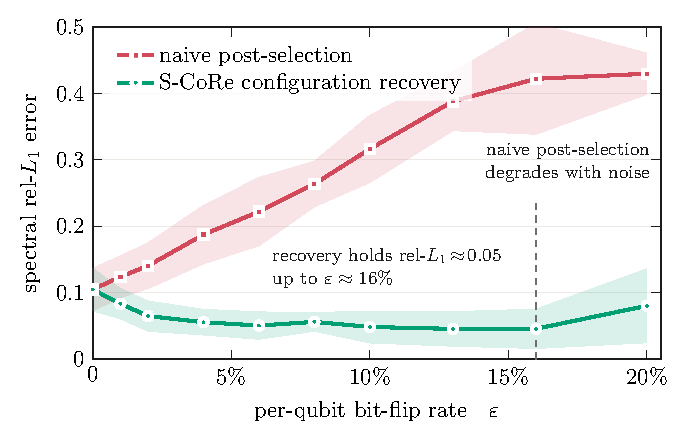
\includegraphics[width=0.7\linewidth]{figs/fig_noise_score.pdf}
\caption{\textbf{Noise robustness (synthetic per-qubit bit-flip channel, $L=6$).} Spectral
relative-$L_1$ error vs the per-qubit bit-flip rate $\varepsilon$, applied to bitstrings Born-sampled from
the exact distribution (this is a controlled classical simulation, not a device run). Naive
post-selection degrades steadily, whereas S-CoRe self-consistent configuration recovery holds the error
near $0.05$ out to $\varepsilon\approx16\%$ (seed-averaged over $6$ seeds at $6{,}000$ shots each; bands
$=\pm1$ s.d.\ across seeds).}\label{fig:noise}\end{figure*}

% carried verbatim from the v2 tree (hardware.tex); NOT part of this session's deliverable.
\begin{figure*}[tp]\centering% self-contained native pgfplots fragment (fig:noiserec)
\definecolor{nrH6}{HTML}{6A4C93}
\definecolor{nrNH3}{HTML}{E8880C}
\definecolor{nrN2}{HTML}{D7263D}
\definecolor{nrCO}{HTML}{12876F}
\definecolor{nrC2}{HTML}{2E6F95}
\definecolor{nrOK}{HTML}{0E7C7B}\definecolor{nrBad}{HTML}{5E4B8B}\definecolor{nrNv}{HTML}{D1495B}\definecolor{nrChem}{HTML}{2E7D32}
\begin{tikzpicture}
\begin{groupplot}[group style={group size=2 by 1, group name=nrg, horizontal sep=1.45cm}, height=9.5cm, paperaxis,
  title style={at={(0,1)},anchor=south west,font=\bfseries,yshift=1pt}]
\nextgroupplot[width=0.505\linewidth, ymode=log, xmin=-1, xmax=31, ymin=3e-3, ymax=80,
  xlabel={per-qubit bit-flip rate $\varepsilon$ (\%)}, ylabel={energy error vs FCI (mHa)}, title={(a)},
  legend style={at={(0.5,0.03)},anchor=south,font=\normalsize,draw=black!20},legend columns=3,legend cell align=left]
\draw[nrChem,dashed,line width=0.6pt] (axis cs:-1,1.6) -- (axis cs:31,1.6);
% chemical-accuracy label: emitted after the groupplot, see below.
\addplot[name path=H6lo,draw=none,forget plot] coordinates {(0,3.2914) (2,3.0066) (5,3.6550) (10,3.7659) (15,5.3712) (20,8.9720) (30,15.6267)};
\addplot[name path=H6hi,draw=none,forget plot] coordinates {(0,4.5041) (2,4.1385) (5,4.4412) (10,6.5199) (15,9.5780) (20,16.7961) (30,29.8587)};
\addplot[nrH6,opacity=0.15,forget plot] fill between[of=H6lo and H6hi];
\addplot[name path=NH3lo,draw=none,forget plot] coordinates {(0,2.1436) (2,1.4495) (5,1.0457) (10,0.7919) (15,1.3563) (20,1.8046) (30,5.7326)};
\addplot[name path=NH3hi,draw=none,forget plot] coordinates {(0,2.9078) (2,1.9853) (5,1.6281) (10,1.6847) (15,2.0580) (20,2.8561) (30,20.1868)};
\addplot[nrNH3,opacity=0.15,forget plot] fill between[of=NH3lo and NH3hi];
\addplot[name path=N2lo,draw=none,forget plot] coordinates {(0,0.1729) (2,0.1550) (5,0.3169) (10,0.2965) (15,0.6158) (20,1.4642) (30,8.4636)};
\addplot[name path=N2hi,draw=none,forget plot] coordinates {(0,0.6006) (2,0.6093) (5,0.6846) (10,1.3158) (15,2.3324) (20,5.5026) (30,17.8734)};
\addplot[nrN2,opacity=0.15,forget plot] fill between[of=N2lo and N2hi];
\addplot[name path=COlo,draw=none,forget plot] coordinates {(0,1.5510) (2,1.5669) (5,1.0491) (10,0.7344) (15,0.5781) (20,0.4698) (30,0.3702)};
\addplot[name path=COhi,draw=none,forget plot] coordinates {(0,1.9155) (2,2.0418) (5,1.4264) (10,1.3026) (15,1.0358) (20,0.7942) (30,1.0249)};
\addplot[nrCO,opacity=0.15,forget plot] fill between[of=COlo and COhi];
\addplot[name path=C2lo,draw=none,forget plot] coordinates {(0,0.1703) (2,0.1351) (5,0.0827) (10,0.0677) (15,0.0479) (20,0.0385) (30,0.0118)};
\addplot[name path=C2hi,draw=none,forget plot] coordinates {(0,0.1967) (2,0.1807) (5,0.1240) (10,0.0817) (15,0.0730) (20,0.0627) (30,0.0433)};
\addplot[nrC2,opacity=0.15,forget plot] fill between[of=C2lo and C2hi];
\addplot[nrH6,line width=1.4pt,mark=*,mark size=1.3pt,mark options={fill=nrH6,draw=white,line width=0.4pt}] coordinates {(0,3.8978) (2,3.5726) (5,4.0481) (10,5.1429) (15,7.4746) (20,12.8840) (30,22.7427)}; \addlegendentry{H$_6$}
\addplot[nrH6,line width=0.9pt,densely dashed,forget plot] coordinates {(0,3.8978) (2,4.6251) (5,5.6347) (10,7.8697) (15,12.9901) (20,23.8560) (30,50.3837)};
\addplot[nrNH3,line width=1.4pt,mark=*,mark size=1.3pt,mark options={fill=nrNH3,draw=white,line width=0.4pt}] coordinates {(0,2.5257) (2,1.7174) (5,1.3369) (10,1.2383) (15,1.7072) (20,2.3304) (30,12.7391)}; \addlegendentry{NH$_3$}
\addplot[nrNH3,line width=0.9pt,densely dashed,forget plot] coordinates {(0,2.5257) (2,2.9622) (5,2.7617) (10,2.9227) (15,3.7294) (20,5.5505) (30,31.5152)};
\addplot[nrN2,line width=1.4pt,mark=*,mark size=1.3pt,mark options={fill=nrN2,draw=white,line width=0.4pt}] coordinates {(0,0.3843) (2,0.3445) (5,0.5007) (10,0.6589) (15,1.3685) (20,3.2538) (30,13.1685)}; \addlegendentry{N$_2$}
\addplot[nrN2,line width=0.9pt,densely dashed,forget plot] coordinates {(0,0.3843) (2,0.4335) (5,0.6929) (10,1.1118) (15,2.8006) (20,6.3706) (30,31.8749)};
\addplot[nrCO,line width=1.4pt,mark=*,mark size=1.3pt,mark options={fill=nrCO,draw=white,line width=0.4pt}] coordinates {(0,1.7332) (2,1.8043) (5,1.2377) (10,1.0185) (15,0.8069) (20,0.6320) (30,0.6975)}; \addlegendentry{CO}
\addplot[nrCO,line width=0.9pt,densely dashed,forget plot] coordinates {(0,1.7332) (2,1.9851) (5,1.9371) (10,1.4901) (15,1.8518) (20,2.5550) (30,2.8339)};
\addplot[nrC2,line width=1.4pt,mark=*,mark size=1.3pt,mark options={fill=nrC2,draw=white,line width=0.4pt}] coordinates {(0,0.1835) (2,0.1579) (5,0.1034) (10,0.0747) (15,0.0604) (20,0.0506) (30,0.0261)}; \addlegendentry{C$_2$}
\addplot[nrC2,line width=0.9pt,densely dashed,forget plot] coordinates {(0,0.1835) (2,0.1635) (5,0.1143) (10,0.0811) (15,0.0746) (20,0.0647) (30,0.0657)};
\nextgroupplot[width=0.425\linewidth, xmode=log, xmin=2.2e-3, xmax=14, enlarge y limits=0.03,
  ytick={0,1,2,3,4,5,6,7,8,9,10,11,12,13,14,15,16,17,18}, yticklabels={BeH$_2$,H$_2$,LiH,HF,F$_2$,H$_2$O,H$_4$,OH,LiF,BH,N$_2$,BeH,C$_2$,NO,O$_2$,CN,CO,NH$_3$,H$_6$}, y tick label style={font=\normalsize},
  xtick={0.01,0.1,1,10}, xticklabels={$0.01$,$0.1$,$1$,$10$}, xminorticks=false,
  xlabel={energy error at $\varepsilon=2\%$ (mHa)}, title={(b)},
  legend style={at={(0.03,0.03)},anchor=south west,font=\normalsize,draw=black!20},legend cell align=left]
\fill[nrChem,fill opacity=0.06] (axis cs:2.2e-3,-0.6) rectangle (axis cs:1.6,18.6);
\draw[nrChem,dashed,line width=0.7pt] (axis cs:1.6,-0.6) -- (axis cs:1.6,18.6);
\node[nrChem,font=\tiny,anchor=south,rotate=90] at (axis cs:1.6,9.5) {};
\draw[black!32,line width=0.8pt] (axis cs:0.0022,0) -- (axis cs:0.0022,0); \draw[black!32,line width=0.8pt] (axis cs:0.0022,1) -- (axis cs:0.0022,1); \draw[black!32,line width=0.8pt] (axis cs:0.0022,2) -- (axis cs:0.0022,2); \draw[black!32,line width=0.8pt] (axis cs:0.0022,3) -- (axis cs:0.0022,3); \draw[black!32,line width=0.8pt] (axis cs:0.0022,4) -- (axis cs:0.0022,4); \draw[black!32,line width=0.8pt] (axis cs:0.0327,5) -- (axis cs:0.0022,5); \draw[black!32,line width=0.8pt] (axis cs:0.3178,6) -- (axis cs:0.0022,6); \draw[black!32,line width=0.8pt] (axis cs:0.0194,7) -- (axis cs:0.0194,7); \draw[black!32,line width=0.8pt] (axis cs:0.0254,8) -- (axis cs:0.0254,8); \draw[black!32,line width=0.8pt] (axis cs:0.0845,9) -- (axis cs:0.0605,9); \draw[black!32,line width=0.8pt] (axis cs:0.0688,10) -- (axis cs:0.0636,10); \draw[black!32,line width=0.8pt] (axis cs:0.1367,11) -- (axis cs:0.1367,11); \draw[black!32,line width=0.8pt] (axis cs:0.1711,12) -- (axis cs:0.1615,12); \draw[black!32,line width=0.8pt] (axis cs:0.3275,13) -- (axis cs:0.1942,13); \draw[black!32,line width=0.8pt] (axis cs:0.4696,14) -- (axis cs:0.3363,14); \draw[black!32,line width=0.8pt] (axis cs:0.7815,15) -- (axis cs:0.7261,15); \draw[black!32,line width=0.8pt] (axis cs:1.3923,16) -- (axis cs:1.2450,16); \draw[black!32,line width=0.8pt] (axis cs:2.6491,17) -- (axis cs:1.5063,17); \draw[black!32,line width=0.8pt] (axis cs:4.3814,18) -- (axis cs:3.5606,18);
\addplot[only marks,mark=o,mark size=1.9pt,nrNv,line width=0.8pt] coordinates {(0.0022,0) (0.0022,1) (0.0022,2) (0.0022,3) (0.0022,4) (0.0327,5) (0.3178,6) (0.0194,7) (0.0254,8) (0.0845,9) (0.0688,10) (0.1367,11) (0.1711,12) (0.3275,13) (0.4696,14) (0.7815,15) (1.3923,16) (2.6491,17) (4.3814,18)}; \addlegendentry{naive}
\addplot[only marks,mark=*,mark size=2.1pt,nrOK] coordinates {(0.0022,0) (0.0022,1) (0.0022,2) (0.0022,3) (0.0022,4) (0.0022,5) (0.0022,6) (0.0194,7) (0.0254,8) (0.0605,9) (0.0636,10) (0.1367,11) (0.1615,12) (0.1942,13) (0.3363,14) (0.7261,15) (1.2450,16) (1.5063,17) (3.5606,18)}; \addlegendentry{S-CoRe}
\node[black,font=\normalsize,anchor=north east] at (axis cs:1.4720000000000002,18.3) {$1.6$ mHa};
\end{groupplot}
\node[nrChem,font=\footnotesize,anchor=south east,inner sep=1pt]
      at (nrg c1r1.north east) {chemical accuracy ($1.6$\,mHa)};
\end{tikzpicture}

\caption{\textbf{SQD ground-state energy under a controlled bit-flip model across the molecular suite.}
\textbf{(a)}~Energy error vs the per-qubit bit-flip rate $\varepsilon$ for five representative molecules
($\mathrm{H_6}$, $\mathrm{NH_3}$, $\mathrm{N_2}$, CO, $\mathrm{C_2}$; seed-averaged over $8$ seeds at $4{,}000$ shots each, bands $=\pm1$ s.d.\ across seeds; log scale). Solid $=$ S-CoRe recovery, dashed $=$ naive
post-selection. The advantage of recovery over naive post-selection, both arms consuming the same corrupted
bitstrings at the same rate with the same seeds, grows with noise. For $\mathrm{CO}$ and
$\mathrm{C_2}$ the error at finite $\varepsilon$ also falls below its own $\varepsilon=0$ value;
that second comparison is not used here (Sec.~\ref{sec:scope:hw}): it is decided by the size of
the recovered subspace, which this sweep does not record. \textbf{(b)}~The full nineteen-molecule suite at a realistic
$\varepsilon=2\%$ (log scale, sorted): for each molecule the naive post-selection error (open circle) is
linked to the S-CoRe value (filled), so the leftward pull is the recovery gain; the shaded band is
chemical accuracy ($<1.6$~mHa). Eighteen of nineteen land inside it; $\mathrm{H_6}$, the most
multireference case, is the residual challenge. Panels (a) and (b) are independent seed ensembles
(panel (a): $8$ seeds; panel (b): $5$ seeds, $4000$ shots), so a given molecule's $\varepsilon=2\%$ value
can differ by up to a factor of a few between them (for $\mathrm{N_2}$, $0.34$ vs $0.06$~mHa; both far below chemical accuracy).}\label{fig:noiserec}\end{figure*}

% ---------------------------------------------------------------------------------
%  fig:amort and fig:gflow are NOT typeset.  This is not a layout decision.
%  Sec. 9.4 of this manuscript reads, in the body: "Both figures of this test are
%  therefore withdrawn and the surviving statement is made in prose."  The same
%  paragraph withdraws the two ratios "3.1 s.d." and "1.2 s.d." because they are
%  a difference divided by one arm's standard deviation and so are not test
%  statistics at all -- and those two numbers are exactly what the caption of
%  fig:gflow asserts.  The header of sec_9.tex says the same thing to the builder:
%  "\ref{fig:gflow} and \ref{fig:amort} are DELIBERATELY ABSENT: both figures are
%  cut here".  Typesetting them anyway printed, three pages after the retraction,
%  the statistics the retraction withdraws; and neither float was referenced by any
%  sentence -- they were the only two orphan floats of the thirty-five.  The two
%  \input lines were carried over from the one-column driver by accident.
% \input{carried/fig_amort.tex}
% \input{carried/fig_gflow.tex}

% =====================================================================================
%  Sec. 10 -- CONCLUSION.  Replaces paper/conclusion.tex in full.
%
%  STRUCTURE, reordered 2026-09-23 and audited after writing.  The content is the same
%  as the previous version of this file; the ORDER is not.  Previously: bound first,
%  vacuity last, so the section read "here is my certificate and it does not work".
%  Now:
%    the OBSTRUCTION as the result  |  the two-sided bound as the instrument that
%    identifies the object obstructed  |  the sweep as the evidence, with the one
%    positive property and its own defeater  |  THREE limits, named and numbered in
%    prose  |  the open question  |  one closing sentence.
%  No promise of advantage anywhere.  The closing sentence must not be turned into one.
%
%  WHAT THIS REORDER MAY NOT DO, and did not: add a claim the manuscript does not
%  already make, turn a hedge into an assertion, or drop a number, a concession, a
%  priority attribution or a retraction.  Two concessions were moved IN from Secs. 3.1
%  and 5 rather than out: the explicit retraction of Theorem 1(iii) of versions 1-2,
%  and the ten-of-fourteen out-of-sample result for the two-parameter rule fitted in
%  1-w_S, with the count that moves between six and twelve.  Both make the section
%  longer and are kept for that reason.
%
%  EXTERNAL LABELS USED (all owned by other sections):
%    thm:leakage, sec:leakage  Sec. 3          [sec_3_body.tex]
%    sec:retraction            Sec. 3.1        [sec_3_1.tex]
%    thm:moments               Sec. 4          [sec_4_body.tex]
%    sec:frontier, sec:frontier:obstruction    [sec_5_body.tex]
%    sec:nogo, thm:witness, prop:leakinv       [sec_6_body.tex]
%    sec:prices                Sec. 7          [sec_7.tex]
%    sec:physics, tab:gaps     Sec. 8          [sec_8.tex]
%    sec:honest                Sec. 9          [sec_9.tex]
%  This file defines only: sec:conclusion.
%
%  \cite keys used here, all VERIFIED PRESENT in paper/bibliography.tex (2026-09-23):
%    benthien2007, nocera2016, kuehner1999, whitefeiguin2004, holzner2011, kpm2006,
%    paeckel2019, tdasci2024, whitedmrg1992, schollwock2011, tarabunga2026.
%  The set is unchanged by the reorder: none added, none dropped.
%
%  GREP NOTES for the mechanical audit:
%   (a) "decoupled"/"decoupling" appear nowhere in this file.
%   (b) The section opens on the obstruction and does not end on one: the three limits
%       are followed by the open question and by what the paper leaves behind.
%   (c) No number retired on 2026-09-18 appears here.  In particular this file does NOT
%       say that the shot budget grows with a larger exponent than the support (Sec. 7
%       measures the difference at 0.054 per site with a 95% interval containing zero),
%       quotes no minimum slack for the bound, and quotes the spin-gap coefficient only
%       as the approximate value of Sec. 8, never to three figures.
%   (d) The headline impossibility carries its scope inside the same sentence ("at every
%       size this work reports"), and the L=6 support count (296 of 300, which is the
%       one size whose answer depends on the threshold) is printed next to it.  Neither
%       may be dropped: without them the sentence claims a theorem the paper does not
%       prove.
% =====================================================================================

\section{Conclusion}
\label{sec:conclusion}

The result of this paper is negative, and it is a statement about the problem rather than about our
inequality: from $L=8$ on, in the determinant basis a device measures in, no leakage-type
certificate---ours or another---can be non-vacuous at low fraction. The reason
is geometric and it is measured. Zero leakage requires the subspace to contain the Krylov space
$\mathcal K(H,\phi)$, and the coordinate support of that Krylov space is $296$ of $300$ determinants
at $L=6$ and all $3920$ of $3920$ at $L=8$---so at $L=8$ the leakage is strictly positive for every
proper coordinate subspace---and, at an amplitude threshold of $10^{-12}$, the whole sector at
$L=8$, $10$, $12$ and $14$, the largest of dimension $10\,306\,296$, by two estimators that agree
wherever both ran (Sec.~\ref{sec:frontier:obstruction}). The obstruction is structural rather than
incidental, and a property of the basis the device measures in, not of the bound and not of the
ranking.

The two-sided bound is what identifies the object that obstruction is about. By
Theorem~\ref{thm:leakage} the error of a spectral function reconstructed on a subspace of sampled
configurations splits into the Born weight the shots failed to capture and the Hamiltonian coupling
that leaks across the boundary of that subspace at the resolution asked for; only the first of the
two is bought by drawing more bitstrings, so the error is indexed on the boundary and not on the
weight. The weight alone cannot carry the statement: no inequality indexed on the captured weight can
hold, by an analytic counterexample and by counting, and the weight-only Theorem~1(iii) of
versions~1 and~2 of this preprint is retracted (Sec.~\ref{sec:retraction}). What a Krylov-adequate
subspace does guarantee is moment exactness through order $2K+1$, with the proof the code realizes
(Theorem~\ref{thm:moments}). And nothing cheaper bounds that boundary \emph{usefully} from outside: one-body
fermionic magic is constant along an orbit on which the determinant support runs from $O(K)$ to
$2^{K}$ at bond dimension $2$, and constant on fibers on which the subspace-aware certificate still
separates (Theorem~\ref{thm:witness}, Proposition~\ref{prop:leakinv}), the general
invariant/basis-dependent division being due to Tarabunga \emph{et al.}~\cite{tarabunga2026}.

Measured subspace by subspace at five system sizes, that bound is vacuous at every published
fraction, at each of the five sizes evaluated, by factors of $1.66$ to $8.61$, converged in Krylov
depth at $L=12$---not an accident of the constants, but the obstruction in the numbers. The same
sweep yields the one positive property that survived four independent attacks: the crossing of the
trivial bound occurs at a true relative $L_1$ error between $1.2\times10^{-3}$ and
$7.3\times10^{-3}$, median $2.8\times10^{-3}$, over sixteen $(L,\eta)$ cells at $L=6$--$12$ and
$\eta=0.10$--$0.25\,t$---a drift, not scatter: ordered without exception in both arguments and
conservative in $L$---and it is computed without the answer (Sec.~\ref{sec:frontier}). Its own limit
is in the same table: a rule with two constants fitted in $1-w_S$ localizes that crossing about as
tightly out of sample and more tightly on ten of the fourteen train/test splits, a count that moves
between six and twelve as the constants are fitted, so we claim no superiority for the certificate as
a tracker of the error against the captured weight---out of sample it has none. The method is priced
on three axes rather than one, the third---shots---measured here for the first time
(Sec.~\ref{sec:prices}), and the primitive is validated against the one answer known exactly and
independently of it: from the same calculation on the same lattice, the charge scale converges to a
finite thermodynamic value while the spin scale closes as $\approx2.1/L$, with an independent
effective-Heisenberg control (Table~\ref{tab:gaps}).

Three limits bound all of it, and we state them as flatly as the results. \emph{First, the
certificate does not certify the reconstructions this paper reports.} They are, at present,
uncertified---vacuous at every published fraction and at each of the five sizes evaluated,
above---and neither a sharper proof nor a rearrangement of the subspace repairs that.
\emph{Second, the largest momentum-resolved spectrum is $L=12$, by exact diagonalization.} The three
momentum-resolved responses reported here were computed classically by dynamical DMRG in
2007~\cite{benthien2007}---at $120$, $100$ and $90$ sites in the charge, spin and single-particle
channels respectively---and at $L=48$ in the Hubbard chain, $L=64$ in the Heisenberg chain, with
correction vectors~\cite{nocera2016}; the wider classical toolbox is broader
still---correction-vector and time-dependent DMRG, Chebyshev matrix-product states and
kernel-polynomial expansions~\cite{kuehner1999,whitefeiguin2004,holzner2011,kpm2006,paeckel2019}, and
the real-time propagation of selected configuration-interaction wavefunctions~\cite{tdasci2024}; one
dimension is where tensor networks, since White's formulation~\cite{whitedmrg1992}, are
near-optimal~\cite{schollwock2011}, and nothing in this work competes with that standard; the
vocabulary of the thermodynamic limit is accordingly absent from it (Sec.~\ref{sec:physics}).
\emph{Third, the certified regime costs more shots than the method saves.} Moving from the published
fraction to the non-vacuous band multiplies the shots per snapshot needed for the marginal
configuration by $7.5$ to $10$ at $L=8$ and by $20$ to $35$ at $L=12$, where that configuration
carries a Born probability of $1$ to $2\times10^{-9}$: a regime a device can certify is, on these
systems, one in which diagonalizing the whole sector is already the cheaper thing to do.

Two questions follow, and only one of them is a matter of more computing. Whether a certified regime
exists at low sector fraction is now a well-posed measurement rather than an expectation, and the
calibration above is the instrument for making it; whether it exists at all turns on a prior question
this work can pose but not answer---whether any single-particle basis leaves the coordinate support
of $\mathcal K(H,\phi)$ short of the entire sector, since it is that support, and not the quality of
the sampler, that pins the threshold measured here.

What this paper leaves behind is therefore narrow and, we think, useful: an obstruction measured
rather than conjectured, binding a class of certificates and not only ours; a two-sided bound that
names the boundary as the object the error is indexed on and can be evaluated without the answer; and
a map of where that bound is informative, its negative half stated in the same voice as its positive
one.

% ---------------------------------------------------------------------------------
%  ACKNOWLEDGMENTS -- added 2026-09-19 at the end of the last body section, which is
%  where REVTeX places this block: main.tex inputs sec_10.tex and then \clearpage
%  \appendix, so the block falls after the Conclusion and before Appendix A.
%
%  WHAT PRA ACTUALLY REQUIRES, checked rather than assumed (2026-09-19):
%    * Data Availability Statement: REQUIRED.  "All published articles must include a
%      Data Availability Statement (DAS)" -- journals.aps.org/pra/authors, and
%      journals.aps.org/authors/data-availability-statements.  Written as Sec. 9.6.
%    * Conflict of interest: NOT required inside the article.  APS requires authors to
%      "alert editors to any potential conflict of interest such as sources of funding,
%      condition of employment, and any limitations on disclosure of data, code, or
%      experimental details", and only ENCOURAGES a statement in the paper itself
%      ("authors are encouraged to declare any conflict of interest within the paper
%      itself using a Conflict of Interest statement") -- journals.aps.org/authors/
%      editorial-policies.  So none is printed here.  If Nicolas wants one, it goes in
%      this block; the employment affiliation is the item an editor would expect named.
%    * Funding: nothing is claimed here, in either direction.  This block asserts only
%      what can be verified from the deposit, i.e. that the device runs happened.
%  The IBM sentence is IBM Quantum's standard acknowledgement and disclaimer.
% ---------------------------------------------------------------------------------
\begin{acknowledgments}
We acknowledge the use of IBM~Quantum services for this work; the two device runs reported in
Sec.~\ref{sec:scope:hw} were executed on \texttt{ibm\_fez} and \texttt{ibm\_marrakesh}. The views
expressed are those of the author and do not reflect the official policy or position of IBM or the
IBM~Quantum team.
\end{acknowledgments}


% The one-column driver carried \FloatBarrier here (main_test.tex:176).  placeins
% is not loaded -- it documents that it does not handle double-column floats -- so
% the barrier is \clearpage, which does flush them.  Without it six body floats of
% Sec. IX were composed inside Appendix A.
\clearpage
\appendix

% ===================================== [APPENDIX] ====================================
%  Move verbatim into the appendix, after the moment appendix of sec_4.tex.
% =====================================================================================

\section{Counterexamples to the weight-only bound, and the pooled sweep}
\label{app:counterex}

\paragraph{The three-level family.} Section~\ref{sec:retraction} exhibits a two-level instance forcing
the constant of the weight-only bound~\eqref{eq:weightonly} to its trivial value at $w_S=1$. With $w_S<1$
strictly the failure is unbounded. Take
$H=\operatorname{diag}\bigl(\bigl(\begin{smallmatrix}0&g\\ g&0\end{smallmatrix}\bigr),\delta\bigr)$,
$\phi=e_0+\varepsilon e_2$ and $S=\{0\}$, so that $1-w_S=\varepsilon^{2}/(1+\varepsilon^{2})$ may be
made as small as wished while the weight displaced to $\pm g$ stays $O(1)$. The ratio of the measured
error to the weight-only bound then diverges as $\delta^{-2}$ in the displacement $\delta$ of the
discarded component; we measured it to $7.6\times10^{7}$ before double precision limits the family.

\paragraph{The pooled sweep behind Fig.~\ref{fig:thm1iii-violation}.} Five machine-readable scans,
written by two independent implementations, contribute $621$ subspaces: $243$ from the original sweep,
and $162+112+104$ from a re-implementation deposited as \texttt{cert\_stress.json},
\texttt{cert\_akw.json} and \texttt{cert\_teqsci.json}. Fifteen reproduce the target to
double-precision round-off (relative $L_1\le10^{-10}$) and define no ratio, leaving $606$ live
subspaces over four Hamiltonian families --- Hubbard chains, XXZ, $t$--$V$, Anderson and sparse random
matrices --- and eight construction rules, of which $156$ are finite-shot realizations at $4000$ shots
per snapshot and the remainder deterministic weight-ordered or structured selections. On those $606$:
the weight-only bound fails on $468$; among the $363$ with $w_S\ge0.99$ --- the regime a sampling
experiment aims for --- it fails on all $363$, the mildest by a factor $2.10$, with $50$ of them carrying $w_S=1$
exactly, so that the bound is identically zero and the ratio infinite; below $w_S=0.99$ it survives on
$138$ of $243$, in every case where the relative error is already of order unity and the bound excludes
nothing. Theorem~\ref{thm:leakage} is violated by none of the $606$; the largest ratio of error to
bound is $0.9999999997$, attained on four subspaces with $w_S=0$ exactly, where $A_S\equiv0$ and the
trivial branch is an identity rather than an inequality. The leakage branch is the smaller of the two
on only $61$ of the $606$: the sweep shows that the bound \emph{holds}, not that it is tight.

\paragraph{Independent re-verification.} The $378$ rows of the three deposited scans were re-audited
for this version by a script sharing no code with the one that produced them. It confirms $378$ of
$378$ for each side of Eq.~\eqref{eq:twobudget}; a largest error-to-bound ratio of $0.9999999997$ over
the $376$ rows that define one; the exclusion lemma~\eqref{eq:exclusion} on $378$ of $378$, with $357$
rows at $K_S=-1$ and $21$ at $w_S=1$ exactly; and violations of the weight-only bound on $219$ of the
$219$ finite-ratio rows with $w_S\ge0.99$, the mildest by a factor $2.00$.

\begin{figure*}[tp]\centering
% ---------------------------------------------------------------------------------------------
% LAYOUT 2026-09-18: panel width 0.455->0.447\linewidth and horizontal sep 1.35->1.15cm.
% Reason: measured with \sbox inside the manuscript geometry the fragment was 480.24pt wide
% fragment to 480.24pt against a 472.32pt text block.  Now 445pt.  Data unchanged.
% Native pgfplots fragment (fig:thm1iii-violation) -- APPENDIX.
% Theorem 1(iii) as published, ||A-A_S||_1 <= 2||phi||^2 (1-w_S) + C rho^{-K_S}, tested against
% the measured L1 error, and compared with the replacement bound (Theorem B).
%
% EVERY coordinate comes from a JSON written by an auto-verifying run; none is typed by hand.
% Builder: build_n3.py -> n3_*.dat ; the counts quoted in the legend are re-checked by that
% script against the .dat files it writes (see n3_summary.json).
%   thm3_results.json  239 rows  original sweep: 3 Hubbard L=6 Hamiltonians x 8 subspace families
%   thm3_L8b.json        4 rows  a SITE-seeded L=8 run.  NOT the paper's Fig. 5 configuration:
%                                 its own docstring says "Site seed instead of momentum seed",
%                                 while release/src/sampled_akw.py seeds with c^dag_{k,up}|GS>.
%                                 Kept in the cloud, never highlighted.
%   cert_stress.json   162 rows  \
%   cert_akw.json      112 rows   > independent re-implementation (certificate.py, 2026-09-18).
%                                 Its 64 L=8 rows ARE the paper's Fig. 5 setting (momentum seeds,
%                                 eta=0.18t, FR=0.50/0.70/0.85/0.95) and reproduce the deposited
%                                 sampled_akw_L8.json to 2.1e-8 absolute; they are the highlighted series.
%   cert_teqsci.json   104 rows  /
% 621 pooled; 15 are exact to machine noise (relative L1 <= 1e-10) and carry no defined ratio.
% The plotted published bound is the weight term 2||phi||^2(1-w_S). On 195 of the 239 rows of the
% original sweep the Krylov order is K_S = -1, so the second term C rho^{-K_S} = C rho supplies no
% decay at all and no finite constant C turns the statement into a bound (2x2 counterexample).
% Theorem B is plotted AS STATED: the minimum of the trivial cap ||phi||^2(1+w_S) and the leakage
% branch (||phi||+||phi_S||)(||phi_Q|| + Lambda_S(eta)/eta). The leakage branch is the smaller of
% the two in only 61 of the 606 live rows -- this figure does NOT show the leakage branch is tight.
% ---------------------------------------------------------------------------------------------
\definecolor{vlHi}{HTML}{D55E00}      % published bound, captured weight w_S >= 0.99
\definecolor{vlLo}{HTML}{E9A178}      % published bound, w_S < 0.99
\definecolor{vlNew}{HTML}{0072B2}     % Theorem B (replacement)
\definecolor{vlInk}{HTML}{1B1B1B}
\definecolor{vlRule}{HTML}{7A7A7A}
\begin{tikzpicture}
\begin{groupplot}[
  group style={group size=2 by 1, horizontal sep=1.35cm},
  width=0.455\linewidth, height=7.4cm, paperaxis,
  ymode=log, ymin=1e-6, ymax=5e7,
  ytick={1e-4,1e-2,1e0,1e2,1e4,1e6},
  extra y ticks={1.6e7}, extra y tick labels={$\infty$},
  extra y tick style={grid=none, tick label style={font=\footnotesize}},
  ymajorgrids, grid style={draw=black!10},
  title style={at={(0,1)},anchor=south west,font=\small\bfseries,yshift=1.5pt},
  label style={font=\small}, tick label style={font=\footnotesize},
]
% =========================== (a) versus subspace fraction ===========================
\nextgroupplot[
  title={(a)~versus subspace fraction},
  xlabel={subspace fraction $|\mathcal{S}|/\dim$},
  ylabel={measured $\|A-A_{\mathcal{S}}\|_1$ / bound},
  xmin=0, xmax=1.03, xtick={0,0.25,0.5,0.75,1},
  legend to name=n3legend, legend columns=3, legend cell align=left,
  legend style={draw=none, fill=none, font=\scriptsize, column sep=7pt, row sep=1.5pt},
]
\fill[vlHi,fill opacity=0.055] (axis cs:0,1) rectangle (axis cs:1.03,8e6);
% --- data (all "forget plot"; legend marks are drawn separately so they stay legible) ---
\addplot[forget plot,only marks,mark=o,mark size=1.15pt,draw=vlLo,line width=0.35pt,draw opacity=0.85]
  table {n3_pub_frac_lo.dat};
\addplot[forget plot,only marks,mark=*,mark size=1.15pt,mark options={draw=none,fill=vlHi,fill opacity=0.62}]
  table {n3_pub_frac_hi.dat};
\addplot[forget plot,only marks,mark=*,mark size=1.0pt,mark options={draw=none,fill=vlNew,fill opacity=0.55}]
  table {n3_thmB_frac.dat};
\addplot[forget plot,only marks,mark=triangle*,mark size=1.9pt,
         mark options={draw=none,fill=vlHi,fill opacity=0.9}]
  table[x=x,y expr=1.6e7] {n3_inf_frac.dat};
% --- paper's Fig.5 configuration (64 rows): drawn as min / median / max at each
% abscissa.  The 64 individual rows are NOT removed from the figure -- they are part of
% the orange w_S>=0.99 series.  As 64 separate diamonds they fused into solid blobs that
% resolved no marker and hid the orange points underneath (reviewer defect D3).
% Caps are drawn at +-3% of the abscissa; that is layout, the y values are the data.
\draw[vlInk,line width=0.5pt] (axis cs:0.5,16.1609) -- (axis cs:0.5,21.0661);
\draw[vlInk,line width=0.5pt] (axis cs:0.485,16.1609) -- (axis cs:0.515,16.1609);
\draw[vlInk,line width=0.5pt] (axis cs:0.485,21.0661) -- (axis cs:0.515,21.0661);
\draw[vlInk,line width=0.5pt] (axis cs:0.7,17.8042) -- (axis cs:0.7,29.9511);
\draw[vlInk,line width=0.5pt] (axis cs:0.679,17.8042) -- (axis cs:0.721,17.8042);
\draw[vlInk,line width=0.5pt] (axis cs:0.679,29.9511) -- (axis cs:0.721,29.9511);
\draw[vlInk,line width=0.5pt] (axis cs:0.85,15.0552) -- (axis cs:0.85,33.7282);
\draw[vlInk,line width=0.5pt] (axis cs:0.8245,15.0552) -- (axis cs:0.8755,15.0552);
\draw[vlInk,line width=0.5pt] (axis cs:0.8245,33.7282) -- (axis cs:0.8755,33.7282);
\draw[vlInk,line width=0.5pt] (axis cs:0.95,22.3768) -- (axis cs:0.95,57.2787);
\draw[vlInk,line width=0.5pt] (axis cs:0.9215,22.3768) -- (axis cs:0.9785,22.3768);
\draw[vlInk,line width=0.5pt] (axis cs:0.9215,57.2787) -- (axis cs:0.9785,57.2787);
\addplot[forget plot,only marks,mark=diamond,mark size=3.0pt,draw=vlInk,line width=0.6pt,mark options={fill=white,fill opacity=1}] coordinates {(0.5,18.5343) (0.7,23.621) (0.85,26.4518) (0.95,29.8719)};
\addplot[forget plot,vlInk,line width=0.9pt,densely dashed,domain=0:1.03,samples=2] {1};
\addplot[forget plot,vlRule,line width=0.4pt,dotted,domain=0:1.03,samples=2] {8e6};
% --- legend proxies ---
\addlegendimage{only marks,mark=o,mark size=2.4pt,draw=vlLo,line width=0.7pt}
\addlegendentry{weight term, $w_{\mathcal S}<0.99$ (243)}
\addlegendimage{only marks,mark=*,mark size=2.4pt,mark options={draw=none,fill=vlHi}}
\addlegendentry{weight term, $w_{\mathcal S}\ge 0.99$ (313)}
\addlegendimage{only marks,mark=*,mark size=2.4pt,mark options={draw=none,fill=vlNew}}
\addlegendentry{Theorem~\ref{thm:leakage}, same $\mathcal S$ (606)}
\addlegendimage{only marks,mark=triangle*,mark size=2.6pt,mark options={draw=none,fill=vlHi}}
\addlegendentry{bound $\equiv 0$: ratio $=\infty$ (50)}
\addlegendimage{only marks,mark=diamond,mark size=3.0pt,draw=vlInk,line width=0.7pt}
\addlegendentry{Fig.~\ref{fig:akwsampled} setting (64): range}
\addlegendimage{vlInk,line width=0.9pt,densely dashed}
\addlegendentry{exact equality: ratio $=1$}
% --- in-panel labels, placed in verified-empty corners (never over a marker) ---
\node[vlHi,font=\scriptsize\bfseries,anchor=north west] at (axis cs:0.025,3.2e6) {bound violated};
\node[vlNew,font=\scriptsize\bfseries,anchor=south west] at (axis cs:0.025,1.1e-5) {bound holds};
% =========================== (b) versus broadening eta ===========================
\nextgroupplot[
  title={(b)~versus broadening},
  xlabel={broadening $\eta/t$},
  xmode=log, xmin=0.021, xmax=1.35,
  xtick={0.03,0.05,0.1,0.2,0.5,0.9}, xminorticks=false,
  log ticks with fixed point, yticklabels={,,}, extra y tick labels={},
]
\fill[vlHi,fill opacity=0.055] (axis cs:0.021,1) rectangle (axis cs:1.35,8e6);
\addplot[only marks,mark=o,mark size=1.15pt,draw=vlLo,line width=0.35pt,draw opacity=0.85]
  table {n3_pub_eta_lo.dat};
\addplot[only marks,mark=*,mark size=1.15pt,mark options={draw=none,fill=vlHi,fill opacity=0.62}]
  table {n3_pub_eta_hi.dat};
\addplot[only marks,mark=*,mark size=1.0pt,mark options={draw=none,fill=vlNew,fill opacity=0.55}]
  table {n3_thmB_eta.dat};
\addplot[only marks,mark=triangle*,mark size=1.9pt,
         mark options={draw=none,fill=vlHi,fill opacity=0.9}]
  table[x=x,y expr=1.6e7] {n3_inf_eta.dat};
% --- paper's Fig.5 configuration (64 rows): drawn as min / median / max at each
% abscissa.  The 64 individual rows are NOT removed from the figure -- they are part of
% the orange w_S>=0.99 series.  As 64 separate diamonds they fused into solid blobs that
% resolved no marker and hid the orange points underneath (reviewer defect D3).
% Caps are drawn at +-6% of the abscissa; that is layout, the y values are the data.
\draw[vlInk,line width=0.5pt] (axis cs:0.18,15.0552) -- (axis cs:0.18,57.2787);
\draw[vlInk,line width=0.5pt] (axis cs:0.1692,15.0552) -- (axis cs:0.1908,15.0552);
\draw[vlInk,line width=0.5pt] (axis cs:0.1692,57.2787) -- (axis cs:0.1908,57.2787);
\addplot[forget plot,only marks,mark=diamond,mark size=3.0pt,draw=vlInk,line width=0.6pt,mark options={fill=white,fill opacity=1}] coordinates {(0.18,22.9909)};
\addplot[vlInk,line width=0.9pt,densely dashed,domain=0.021:1.35,samples=2] {1};
\addplot[vlRule,line width=0.4pt,dotted,domain=0.021:1.35,samples=2] {8e6};
\end{groupplot}
\node[anchor=north,yshift=-0.92cm] at (group c1r1.south east) {\pgfplotslegendfromname{n3legend}};
\end{tikzpicture}

% Caption for fig_thm1iii_violation_native.tex  (appendix figure).
% Every number below is traceable to the JSON sources.  The counts, factors and ratios
% are printed by build_n3.py; the two exceptions are 156 and 4000, which that script does
% NOT emit and which fix_n3_caption.py re-derives here from the deposited files:
%   156  = 104 live rows of p2_calc/out/cert_teqsci.json  +  52 rows of thm3_results.json
%          carrying kind = teqsci
%   4000 = cert_teqsci.json /shots (= 4000), the same value as thm3_run.py:28
% The min/median/max whiskers of the Fig.-5 series come from n3_fig5_summary.json,
% written by fix_n3_fig5_series.py from n3_fig5_frac.dat / n3_fig5_eta.dat.
\caption{\textbf{A bound indexed on the captured weight alone fails on exactly the subspaces this work relies on; Theorem~\ref{thm:leakage} does not.}
For each subspace $\mathcal S$ we plot the measured error $\|A-A_{\mathcal S}\|_1$ divided by the
bound, so every point above the dashed line at $1$ is a violation. Orange: the weight term of Eq.~\eqref{eq:weightonly}, $2\|\varphi\|^{2}(1-w_{\mathcal S})$, split by captured weight (filled, $w_{\mathcal S}\ge
0.99$; open, $w_{\mathcal S}<0.99$). Blue: Theorem~\ref{thm:leakage} as stated, $\min\{\|\varphi\|^{2}(1+w_{\mathcal
S}),\,(\|\varphi\|+\|\varphi_{\mathcal S}\|)(\|\varphi_{\mathcal Q}\|+\Lambda_{\mathcal
S}(\eta)/\eta)\}$, on the same subspaces. We pooled $621$ subspaces from five machine-readable
sweeps written by two independent implementations ($239+4$ from the original sweep; $162+112+104$
from an independent re-implementation); $15$ of them reproduce the target to within double-precision
round-off (relative $L_1\le 10^{-10}$) and define no ratio, leaving $606$ live subspaces, of which
$156$ are finite-shot realisations at $4000$ shots per snapshot and the remainder are deterministic
weight-ordered or structured selections. \emph{The weight term alone is violated on $468$ of the $606$.} On $50$ of them it is identically zero: those subspaces carry the whole weight to double
precision ($w_{\mathcal S}=1$ exactly, and $K_{\mathcal S}\in\{0,1,2\}$, so the remaining term is the
undefined constant $C\rho^{-K_{\mathcal S}}$); their ratio is infinite and they are drawn on the row
marked $\infty$, above the dotted rule. Among the $313$ finite-ratio points with $w_{\mathcal S}\ge
0.99$---the regime the paper invokes---\emph{every one} is a violation, the mildest by a factor
$2.10$; with the $50$ infinite ones that is $363$ of $363$, and the finite factors reach
$3.66\times10^{6}$. Below $w_{\mathcal S}=0.99$ the bound survives on $138$ of $243$ points, but only
where the relative error is already of order unity, so it excludes nothing there. Diamonds mark the
configuration of Fig.~\ref{fig:akwsampled} ($L=8$, $U/t=8$, $\eta=0.18t$, momentum seeds
$c^{\dagger}_{k\uparrow}|\Psi_0\rangle$, subspace fractions $0.50/0.70/0.85/0.95$, both branches,
eight momenta): that reconstruction reproduces the deposited \texttt{sampled\_akw\_L8.json} to
$2.1\times10^{-8}$ per momentum, and its violation factor is $15.1$--$57.3$, of which $15.1$--$33.7$
at the fraction $0.85$ of Fig.~\ref{fig:akwsampled}. Those $64$ rows sit at only four abscissae, so they are drawn as a min--median--max whisker at each one rather than as $64$ overlapping markers (medians $18.5, 23.6, 26.5, 29.9$ at fractions $0.50, 0.70, 0.85, 0.95$); each of them is also plotted individually inside the filled orange series, which is where their scatter can be read. Theorem~\ref{thm:leakage} is violated on none of the $606$; its ratios span
$1.18\times10^{-5}$ to $0.9999999997$. That maximum is reached on four subspaces with $w_{\mathcal
S}=0$ exactly, where $A_{\mathcal S}\equiv 0$ and $\|A-A_{\mathcal S}\|_1=\|\varphi\|^{2}$ equals the
trivial cap by algebra---the branch that carries no information---and the leakage branch
$\Lambda_{\mathcal S}(\eta)/\eta$ is the smaller of the two on only $61$ of the $606$ rows: the
figure shows that Theorem~\ref{thm:leakage} \emph{holds}, not that it is tight. In (b) the $\eta$ axis is not a sweep
within one model: the Hubbard-chain rows exist only at $\eta/t=0.05,\,0.15,\,0.18$ and the stress
families (XXZ, $t$--$V$, Anderson, sparse random) only at $0.03,\,0.07,\,0.22,\,0.40,\,0.90$, so no
trend across the full axis may be read from it.}
\label{fig:thm1iii-violation}

\end{figure*}


% ===================================== [APPENDIX] ====================================

\section{Moment exactness: statement, proof, sharpness, and the shot count}
\label{app:moments}

We make precise the two things a Krylov-adequate subspace does deliver. Fix the seed
$\ket{\phi}=\hat c^{\dagger}_{p}\ket{0}$ (the electron-addition branch; removal is identical), with
weight $\lVert\phi\rVert^{2}=\braket{\phi|\phi}$, and let
$A(\omega)=\sum_{n}\lvert\braket{n|\phi}\rvert^{2}\,\mathcal L_{\eta}\!\big(\omega-(E_n-E_0)\big)$ be
the exact spectral function, where $\{\ket{n},E_n\}$ diagonalize $H$ in the $(N{+}1)$-particle sector
and $\mathcal L_{\eta}(x)=\tfrac{\eta/\pi}{x^{2}+\eta^{2}}$. For a configuration set $\mathcal S$ let
$P=P_{\mathcal S}$ be the orthogonal projector onto $\operatorname{span}(\mathcal S)$, let
$H_{\mathcal S}=PHP$ with eigenpairs $\{\ket{\tilde m},\tilde E_m\}$, and let
$A_{\mathcal S}(\omega)=\sum_{m}\lvert\braket{\tilde m|\phi}\rvert^{2}\,
\mathcal L_{\eta}\!\big(\omega-(\tilde E_m-E_0)\big)$ be the reconstruction. Write
$\mathcal K_K=\operatorname{span}\{\phi,H\phi,\dots,H^{K}\phi\}$ and
$w_{\mathcal S}=\lVert P\phi\rVert^{2}/\lVert\phi\rVert^{2}$. Moments are taken on the point measures
$d\mu=\sum_n\lvert\braket{n|\phi}\rvert^{2}\delta(\omega-(E_n-E_0))$ and
$d\mu_{\mathcal S}=\sum_m\lvert\braket{\tilde m|\phi}\rvert^{2}\delta(\omega-(\tilde E_m-E_0))$, not on
the broadened $A$, whose moments of order $\ge2$ diverge.

\subsection{What the proof uses}
\label{app:moments:exact}

Theorem~\ref{thm:moments} and its proof are stated in Sec.~\ref{sec:moments:exact}. The proof uses
$P=P^{\dagger}=P^{2}$, $H=H^{\dagger}$ and $\mathcal K_K\subseteq\operatorname{span}(\mathcal S)$, and
nothing else. In particular it does not use that $\mathcal S$ is a coordinate subspace, that it was
obtained by drawing bitstrings, or that any Lanczos basis is well
conditioned~\cite{epperly2022}; it holds verbatim for
the orthogonal projector onto a Krylov space, which is the form evaluated in Sec.~\ref{sec:frontier}.
The single asymmetry in Eq.~\eqref{eq:rrsplit}---$a$ runs to $K$ while $b$ runs to $K+1$---is what
produces the odd reach $2K+1$ rather than $2K$. Two structural remarks follow at no cost.

\emph{(a) The node count.} $d\mu_{\mathcal S}$ has $|\mathcal S|$ atoms, one per Ritz pair, not $K+1$.
Equation~\eqref{eq:momex} is therefore a weak quadrature statement for a rule of that size: a Gauss
rule of $n$ nodes for $d\mu$ is exact through order $2n-1$~\cite{golub2010}, so the $K=1$ row of
Table~\ref{tab:moments}, with $280$ nodes, would reach order $559$ if its nodes were the Gauss nodes of
$d\mu$. They are not, and it reaches order $3$; those $555$ orders measure the distance between the
two objects. This is the measurable content of the distinction: identifying $A_{\mathcal S}$ with an order-$(K{+}1)$ Gauss rule misdescribes the
object and the reach such an object would have; the reach $2K+1$ of
Theorem~\ref{thm:moments} itself is unaffected.

\emph{(b) Unit captured weight is implied, not assumed.} For a coordinate subspace $P$ is diagonal, so
$P\phi=\phi\iff\operatorname{supp}(\phi)\subseteq\mathcal S\iff w_{\mathcal S}=1$. Since
$\mathcal K_0=\operatorname{span}\{\phi\}$, the hypothesis of Theorem~\ref{thm:moments} at any $K\ge0$
already implies $w_{\mathcal S}=1$. Every subspace admissible for moment exactness therefore sits at
the extreme of the weight budget of Sec.~\ref{sec:leakage}, where the shot term vanishes identically
and the whole residual error is leakage---which is why the two statements are complementary rather
than competing.

\subsection{Sharpness, control, and the limits of the validation system}
\label{app:moments:sharp}

Table~\ref{tab:moments} is computed by exact diagonalization of the $(N{+}1,S_z{=}{+}1)$ sector of the
open $L=6$, $U/t=8$ Hubbard chain ($D=300$, $\lVert\phi\rVert^{2}=1/2$), with
$\mathcal S=\bigcup_{a\le K}\operatorname{supp}(H^{a}\phi)$. Four measurements support it.

\emph{Reach.} Through order $2K+1$ the relative discrepancy is $\le3.2\times10^{-15}$ for $K=0,1$ and
$\le7.5\times10^{-15}$ for $K=2$. At order $2K{+}2$ it is $9.5\times10^{-4}$ ($K=0$) and
$6.0\times10^{-8}$ ($K=1$), eleven and seven decades above the arithmetic floor. The absolute
discrepancies at that order, $3.104583\times10^{-2}$ and $1.340167\times10^{-4}$, agree to six
significant figures across all six implementations listed below and are properties of the
construction, not of the arithmetic. The $K=2$ row carries no entry there, for a structural reason and
not a numerical one: the ladder has filled the sector, $A_{\mathcal S}=A$ identically, and their
relative $L_1$ distance is $0$ to machine arithmetic. One run of one of the six routes does report a
nonzero residue in that row; the same run reports a cyclic-subspace dimension of $301$ inside a sector
of dimension $300$ and emits floating-point overflow while forming the high powers. It is discarded,
and the corrected run is the one quoted.

\emph{Reproducibility of the residues.} The relative discrepancies are quoted, and the absolute ones
below order $2K{+}2$ are not, for a reason worth recording. The exact moments
$\mu_j=\braket{\phi|(H-E_0)^{j}|\phi}$ run from $5.0\times10^{-1}$ at $j=0$ to $1.6\times10^{5}$ at
$j=6$, so an absolute residue at the top of the ladder is a roundoff quantity whose size depends on the
route taken to the same identity. Across six equivalent routes---Rayleigh--Ritz on the shifted or on
the unshifted matrix, crossed with exact moments obtained from the Lehmann sum, from the shifted
matrix--vector recursion, or by binomial recombination of unshifted powers---the relative residue below
order $2K{+}2$ stays inside $[1.1,1.8]\times10^{-15}$ at $K=0$ and $[1.0,3.2]\times10^{-15}$ at $K=1$,
a spread under a factor $3.3$, while the absolute residue at the same orders is not stable to two
significant figures. We therefore quote relative residues below $2K{+}2$, and absolute ones only at
$2K{+}2$, where the discrepancy is physical and route independent.

\emph{Negative control.} Over $300$ uniformly drawn coordinate subspaces of the same size
$|\mathcal S|=200$, the zeroth moment is wrong by between $1.86\times10^{-2}$ and $4.18\times10^{-1}$
(median $1.67\times10^{-1}$), i.e.\ by $3.7\%$ to $84\%$ of $\lVert\phi\rVert^{2}$ (median $33\%$),
with every one of
the $300$ draws failing; the Krylov-support subspace of identical size is exact to
$4.4\times10^{-16}$. At $|\mathcal S|=280$ the random draws fail by $4.8\times10^{-5}$ to
$2.6\times10^{-1}$ (median $1.12\times10^{-2}$), again without exception, against
$5.0\times10^{-16}$. The discriminating variable is the identity of the determinants, not their number.

\emph{Scale.} The Krylov ladder at $L=6$ occupies $0.667$, $0.933$ and $1.000$ of the sector at
$K=0,1,2$, so it exhausts the sector at $K=2$ and the table has exactly three rows. This system can
verify Eq.~\eqref{eq:momex} and locate its exact reach; it cannot exhibit the behaviour of
$\lVert A-A_{\mathcal K_K}\rVert_1$ at large $K$, which is the regime Conjecture~\ref{conj:geom}
concerns, and we make no claim there.

\emph{Why the open chain.} The ladder terminates when the coordinate subspace contains the cyclic
subspace generated by $\phi$---not when it fills the sector---and at that point the reconstruction is
exact, because $\operatorname{span}(\mathcal S)$ then carries every eigenvector of nonzero Lehmann
weight. On the periodic rings of Sec.~\ref{sec:prices} that happens early: at $L=6$ the ladder runs
$200\to296$ and stalls at $296$ of $300$ determinants, where $A_{\mathcal S}=A$ to
$1.0\times10^{-14}$ in relative $L_1$ and the moments are exact past order $2K{+}1$ at every $K\ge1$.
The ring therefore offers a single row in which the reach of Eq.~\eqref{eq:momex} is visible at all
($K=0$: relative discrepancy $4.4\times10^{-16}$ through order $1$, $4.6\times10^{-3}$ at order $2$);
the open chain offers two, and is the system on which the method validation of Sec.~\ref{sec:method} is
performed. Within the reach they cover, both agree: the identity is exact, sharp at the next order, and
decidable from the subspace alone.

\subsection{The geometric-convergence claim, and why it is left open}
\label{app:moments:conj}

Conjecture~\ref{conj:geom} is easily taken for a consequence of Eq.~\eqref{eq:momex}. It is not
one: moment exactness gives $2K+2$ linear identities, and $\lVert A-A_{\mathcal K_K}\rVert_1$ is not a
finite linear functional of them. A proof would require (i) a polynomial approximation theorem for
$x\mapsto\mathcal L_\eta(\omega-x)$, uniform in $\omega$, on a real set containing
$\operatorname{spec}(H)$ and $\operatorname{spec}(H_{\mathcal K_K})$, and (ii) a tail estimate
controlling the complement. For (i) the natural route is a Bernstein-ellipse bound, in which the
resolution enters through the poles of the kernel at $x=\omega\pm i\eta$: the largest admissible
ellipse has semi-minor axis below $\eta$, so its parameter---and with it any geometric rate---approaches
$1$ as $\eta\to0^{+}$. That is a mechanism and not a derivation: it exhibits neither $C(\eta)$
nor $\rho(\eta)$, and neither appears anywhere in this work or in the deposit.

The prefactor is moreover pinned from below by the two-level family of Sec.~\ref{sec:retraction}. With
$H=\bigl(\begin{smallmatrix}0&g\\ g&0\end{smallmatrix}\bigr)$ and $\phi=e_0$ one has
$\braket{\phi|H|\phi}=0$, so $\mathcal K_0=\operatorname{span}\{\phi\}$ carries a single pole at the
origin while $A$ carries two at $\pm g$; by adaptive integration over the whole line at $\eta=0.15$ (\texttt{src/moments\_table.py}), $\lVert A-A_{\mathcal K_0}\rVert_1=1.5197,\ 1.8352,\ 1.9504,\ 1.9835,\ 1.9950,\ 1.9983,\ 1.9995$ for
$g=1,3,10,30,100,300,1000$ at $\lVert\phi\rVert^{2}=1$, approaching the trivial ceiling
$2\lVert\phi\rVert^{2}=2$ monotonically. Any $C(\eta)$
valid uniformly on this family therefore satisfies $C(\eta)\ge2\lVert\phi\rVert^{2}$. A geometric bound
with a trivial prefactor is not worthless---it would still decay in $K$---but it cannot be non-vacuous
at small $K$, and small $K$ is where a shot-limited subspace lives.

Conjecture~\ref{conj:geom} therefore remains open, and we name its two missing ingredients
explicitly so that it can be attacked rather than left unremarked. What this work offers in its place
is not a rate in $K$ at all but a bound on $\lVert A-A_{\mathcal S}\rVert_1$ itself, at the $\eta$ of
the figure and on the subspace actually in hand (Theorem~\ref{thm:leakage}), measured subspace by
subspace, together with a measurement of where that bound is non-vacuous (Sec.~\ref{sec:frontier}).
That is a weaker statement than a rate and a stronger one than a conjecture, and it is the one the
deposit can reproduce.

\subsection{The sample-complexity bound}
\label{app:moments:shots}

\begin{proposition}[Sampling capture]
\label{prop:shots}
Let $p(x)=\tfrac{1}{K+1}\sum_{k=0}^{K}\lvert\braket{x|e^{-iHt_k}\phi}\rvert^{2}/
\lVert\phi\rVert^{2}$, draw $T$ bitstrings independently from $p$, and let $\mathcal S$ be the
set of distinct outcomes. For $\varepsilon,\delta\in(0,1)$, if
$T\ge\varepsilon^{-1}\log\bigl(1/(\varepsilon\delta)\bigr)$ then with probability at least $1-\delta$
the set $\mathcal S$ contains every configuration $x$ with $p(x)\ge\varepsilon$.
\end{proposition}

\begin{proof}
Let $\mathcal N_\varepsilon=\{x:p(x)\ge\varepsilon\}$. Since $\sum_x p(x)=1$ and each member
contributes at least $\varepsilon$, $|\mathcal N_\varepsilon|\le1/\varepsilon$. For fixed
$x\in\mathcal N_\varepsilon$, $\Pr[x\notin\mathcal S]=(1-p(x))^{T}\le(1-\varepsilon)^{T}\le
e^{-\varepsilon T}$. A union bound gives
$\Pr[\mathcal N_\varepsilon\not\subseteq\mathcal S]\le\varepsilon^{-1}e^{-\varepsilon T}$, which is at
most $\delta$ for the stated $T$.
\end{proof}

The cardinality bound $|\mathcal N_\varepsilon|\le1/\varepsilon$ is deterministic, and it is what
removes the circularity of the form $T=O(\varepsilon^{-1}\log(|\mathcal S|/\delta))$, in
which the random size of the sampler's own output appears inside a bound on the number of draws that
produce it. Where $\varepsilon^{-1}\le|\mathcal S|$, the new logarithm is also the smaller one, so
nothing is lost.

The scope of $\varepsilon$ needs the same care. It thresholds a Born probability of the time-averaged
mixture, and Proposition~\ref{prop:shots} makes no statement about $\lVert A-A_{\mathcal S}\rVert_1$.
Two independent obstructions stand between the two quantities. First, the weight left uncaptured is
bounded only by $|\{x:p(x)<\varepsilon\}|\cdot\varepsilon$, which for a delocalized state is $O(1)$:
many small probabilities can sum to most of the mixture. Second, and decisively, a subspace holding the
\emph{entire} Born support of the probe---$w_{\mathcal S}=1$ exactly, nothing left to capture at any
$\varepsilon$---still has relative $L_1$ error $0.28$ at $L=6$ on the open chain of
Table~\ref{tab:moments}, and $0.43$ at $L=6$ and $0.35$ at $L=8$ on the periodic rings, all at
$\eta=0.18\,t$ and all relative to $\lVert\phi\rVert^{2}$ (Sec.~\ref{sec:leakage}); it is the $K=0$
row of Table~\ref{tab:moments}.
Proposition~\ref{prop:shots} is a statement about the sampler and about nothing else. The spectral
error at fixed $\eta$ is the subject of Theorem~\ref{thm:leakage}, and what the composition of the two
actually costs is reported as three separate prices in Sec.~\ref{sec:prices}.

% =====================================================================================
%  DROP-IN CAPTION REPLACEMENT for panel (b) of \ref{fig:method} (results.tex lines 46-51).
%  Not part of Sec. 4; move into the figure file.  It removes the sentence that calls the
%  geometric collapse "guaranteed by the moment-exactness theorem" -- Sec. 4 withdraws that
%  corollary -- and it attaches the shot budget to the word "sampled".
%
% \textbf{(b)}~Relative-$L_1$ error against the number of measured time slices $K$, for the
% finite-shot reconstruction: multinomial draws at $4000$ shots per step, eight independent
% seeds (band $=$ standard deviation), $\eta=0.15\,t$, so the budget is $T=4000(K{+}1)$ and
% reaches $5.2\times10^{4}$ at $K=12$. The error falls by a factor $32$ across the thirteen
% points, from $0.59$ at $K=0$ to $0.0185$ at $K=12$, with one non-monotone step at $K=3$
% inside the discovery phase, while the mean subspace returned grows from $75$ to $242$
% determinants of the $300$-dimensional sector. A geometric rate fitted to the window
% $4\le K\le9$ is withdrawn in Sec.~\ref{sec:moments:notbuy}: it is not implied by moment
% exactness, and inside that window the decay in $K$ is confounded with the growth of
% $|\mathcal S|$.
% =====================================================================================


% ===================================== [APPENDIX] ====================================

\section{The leakage certificate: hypotheses, protocol, and the anatomy of the threshold}
\label{app:hyp}

Theorem~\ref{thm:leakage} holds under three hypotheses. Each is a statement about the pipeline that
produced the reconstruction rather than about the theorem, so each has to be checked against the
pipeline. We check all
three here, with numbers, for the sweep of Sec.~\ref{sec:frontier}, and add the two protocol
declarations and the decomposition that section quotes.

\paragraph{(H1) Common origin.} $A$ and $A_P$ must be referred to the same $E_0$. A shift common to
both cancels exactly---verified to $1.000000$ for shifts of $10^{-3}$, $10^{-2}$ and
$10^{-1}\,t$---which is how the hypothesis is satisfied here, a single $E_0$ being used for both
objects. If $A_P$ is instead referred to $E_0+\delta$, the discrepancy acquires an additive
$\lVert\phi_P\rVert^{2}(4/\pi)\arctan(\lvert\delta\rvert/2\eta)$, verified to $2\times10^{-5}$ in all
$48$ cases tested, \emph{which the certificate does not control}. A ground state obtained by
Rayleigh--Ritz on $60\%$ of the $N$-electron sector at $L=8$ gives $\delta=6.7\times10^{-4}\,t$, which
adds $0.0024$ to a bound of $1.2036$---$+0.20\%$---while multiplying the \emph{measured} error by
$16$; and the dependence is not even monotone, a shift of $10^{-2}\,t$ lowering the measured error at
$L=6$, fraction $0.85$, $\eta=0.18\,t$ from $2.7\times10^{-2}$ to $1.2\times10^{-2}$. The measured
errors quoted beside a bound in Sec.~\ref{sec:frontier} are therefore those of a pipeline handed the
exact $E_0$, and they bound the error of a pipeline that estimates it from neither side. No cheap a
posteriori control on $\delta$ is available: residual (Weinstein) and Temple
bounds~\cite{weinstein1934,temple1928} computed on
ground-state subspaces of $20$--$80\%$ of the $N$ sector at $L=6$ give $\arctan$ terms of $1.76$,
$1.64$, $1.40$ and $0.92$, all vacuous against the ceiling of $2$. In a shot-based pipeline $E_0$ is
itself estimated on whatever subspace the shots populated, and the certificate has never been tested
that way.

\paragraph{(H2) Normalization and support of the $L_1$ norm.} The bound is on
$\int_{\mathbb R}\lvert A-A_P\rvert\,d\omega$ normalized by
$\lVert\phi\rVert^{2}=\int_{\mathbb R}A\,d\omega$. A relative error normalized instead by $\int_W A$
over a finite window $W$ and evaluated by finite quadrature---the convention of the repository, in
which Sec.~\ref{sec:prices} reports---is a different quantity, differing by the product of
$\int_W\lvert A-A_P\rvert/\int_{\mathbb R}\lvert A-A_P\rvert$ and $\lVert\phi\rVert^{2}/\int_W A$.
Both factors are measured here: the second is $1.0100$, $1.0309$ and $1.0373$ at $\eta=0.05$, $0.15$
and $0.18\,t$ at $L=6$ and $1.0110$, $1.0278$ and $1.0335$ at $L=8$, while the first lies between
$1.0040$ and $1.0115$ across the $204$ configurations of this study. Every number in
Sec.~\ref{sec:frontier} is in the normalization of Theorem~\ref{thm:leakage}, and the two conventions
are nowhere interchanged.

\paragraph{(H3) Exact reference.} $A$ denotes the exact spectral function of the full $(N\pm1)$
sector. If the reference is itself a Lanczos reconstruction of finite depth $n_\ell$, the theorem does
\emph{not} bound $\lVert A^{(n_\ell)}-A_P^{(n_\ell)}\rVert_1$, and a measured error below the
reference's own drift measures the reference rather than the reconstruction. That drift runs from
$2.6\times10^{-5}$ ($L=12$, $\eta=0.10\,t$) to $2.8\times10^{-7}$ ($\eta=0.18\,t$), and at $L=10$ the
reorthogonalization gap, $1.71\times10^{-5}$, is of the same order as the depth drift. We therefore
quote no measured error anywhere in Sec.~\ref{sec:frontier} within a factor of $20$ of its own
reference drift: twelve rows at $L\ge10$ fall under that rule and are left blank rather than rounded,
the weakest surviving cell---$L=12$, $\eta=0.10\,t$---standing at a factor $47$. One gap is declared
and not bounded. The reconstructions this paper publishes are produced by bare Lanczos at depth $150$,
while the certificate is evaluated on the reorthogonalized Krylov space; the difference between the
two has been measured at a single point at $L=8$---relative $L_1$ of $1.2454\times10^{-3}$ against
$1.2464\times10^{-3}$---and never bounded, and at $L=12$ it has never been measured at all.

\paragraph{Ranking, ties and support.} Two properties of the cut are declared with the protocol. Only the reflection-forbidden determinants ($4$, $18$, $48$, $200$ at $L=6$--$12$) carry exactly zero accumulated Born weight, and they rank last, so the cut is never filled with configurations the
device would never sample in the infinite-shot limit; ties at the cut involve two determinants (four
at $L=6$, at fractions $0.80$ and $0.85$) and move the bound by at most $6.6\times10^{-4}$ relative.
Above the support floor $\lvert\operatorname{supp}(\phi)\rvert/D$ of Sec.~\ref{sec:retraction}, on the other hand, the
ranking selects among determinants outside $\operatorname{supp}(\phi)$: at fraction $0.85$ that is
$30.2\%$ of $S$ at $L=6$, $42.0\%$ at $L=8$ and ${\approx}39.6\%$ at $L=10$. Those contribute nothing
to $w_S$, and they do change $H_S$. The depth uncertainty quoted in Sec.~\ref{sec:frontier} is the
full recomputation of $\mathrm{FR}^{\ast}$ with $L=12$ capped at $n_\ell=300$: it moves by $0.0024$,
$0.0021$, $0.0012$ and $0.0000$ at $\eta=0.10$, $0.15$, $0.18$ and $0.25\,t$.

\paragraph{Reorthogonalization and the certified object.} Full reorthogonalization is used at every
point of the sweep, without which the projector is not a projector: the orthogonality defect is at
most $4.7\times10^{-15}$, and $P_{\mathcal K}\phi=\phi_S$ to $1.1\times10^{-14}$. At $L=12$ the
certificate is evaluated at $n_\ell=300$--$500$ on up to $658\,627$ determinants, the dense $A_S$
never being formed---which is why what the bound controls is $A_{\mathcal K}$ at the declared depth
and not $A_S$ (Sec.~\ref{sec:frontier:hyp}).

\paragraph{Anatomy of the displacement.} The percentages quoted in
Sec.~\ref{sec:frontier:obstruction} are medians over $15$ of the $18$ $(\eta,\text{target})$ cells at
$L=8$; three cells are censored from above, the certificate never reaching the target inside the grid,
and are excluded rather than imputed. Pooling $L=6$ with $L=8$ shifts them to $52\%$, $31\%$, $11\%$
and $4.1\%$, which is why the $L=8$ figures are the ones quoted. One caveat travels with them, and it
is why they are reported as a diagnosis and not as a quantity: of the rungs of the inequality chain
only the last is computable by a user from $(H,S,\phi,\eta)$, so the decomposition is of an object the
user never sees.


%  APPENDIX MATERIAL BELONGING TO SEC. 6.  Everything below this line is NOT
%  part of the body section: move it verbatim into the appendix file, where it
%  must carry \label{app:witness} (that label already exists in theorem_b2.tex
%  and is reused here for the same content).  Sec. 6 references it twice.
% =============================================================================
\section{The geminal witness: proof and angle sweep}
\label{app:witness}

\begin{proof}[Proof of Theorem~\ref{thm:witness}]
Each geminal occupies its own four spin-orbitals, so \eqref{eq:apsg} is a product across the $K$ blocks
and $\gamma$ is block diagonal with spatial natural occupations
$(n_{b_i},n_{a_i})=(2\cos^2\theta,2\sin^2\theta)$; hence $N_{\mathrm u}=8K\cos^2\theta\sin^2\theta=2K$ at
$\theta=\pi/4$, and $\mathcal F_1=4K$ by Eq.~\eqref{eq:collapse}. The Majorana covariance is likewise
block diagonal, and at $\theta=\pi/4$ a single maximally-paired geminal is the two-determinant cat, whose
covariance vanishes identically ($\Gamma=0$): every order saturates its maximum,
$\mathcal F_k=2n_{\rm o}=4$ per geminal for all $k$, giving $\mathcal F_2=4K$. This equality of orders is
a knife-edge of maximal pairing; away from it the orders separate ($\theta=\pi/6$ gives
$\mathcal F_1=3$, $\mathcal F_2=3.75$ per pair, both still large on the same family). In the pairing basis
each geminal is a two-configuration superposition, so the product carries $2^{K}$ determinants. Finally,
as a product of two-orbital factors the state is a matrix-product state whose every bond crosses at most
one geminal, so $\chi=2$ in that ordering, and contraction and Born sampling then cost $O(K)$. All four
values are reproduced by exact diagonalization for $K=1,\dots,4$.
\end{proof}

Table~\ref{tab:fibersweep} continues the fiber exhibit of Table~\ref{tab:fiber} into a continuous sweep of
the rotation angle at $K=3$. It stops at $s=0.654$: at the maximal-pairing angle $s=\pi/4$ the Born
distribution of $\phi$ is exactly flat over $2^{K}$ determinants, so the top-$|\mathcal S|$ rule does not
select a subspace and no contrast measured there is well defined. Across every row the captured weight is
identical at the two endpoints to $2.2\times10^{-16}$, so the entire difference sits in the leakage term,
and the certificate at the rotated endpoint is the trivial bound $1+w_S$ in every row.

\begin{table*}[tp]\centering\small
\caption{\textbf{Angle sweep of the fiber exhibit}, $K=3$, $\delta=0.01$, $\eta=0.10$,
$|\mathcal S|=4$. Columns as in Table~\ref{tab:fiber}.}
\label{tab:fibersweep}
\setlength{\tabcolsep}{4pt}
\begin{tabular}{@{}lccccc@{}}
\toprule
$s$ & $w_S$ (both endpoints)
 & $\widehat\Lambda/\eta$ al. & $\widehat\Lambda/\eta$ rot.
 & cert.\ al. & cert.\ rot. \\
\midrule
$0.131$ & $0.982963$ & $0.328$ & $1.610$ & $\mathbf{0.913}$ & $1.983$ (trivial) \\
$0.262$ & $0.933013$ & $0.317$ & $3.010$ & $\mathbf{1.131}$ & $1.933$ (trivial) \\
$0.393$ & $0.853553$ & $0.299$ & $4.124$ & $\mathbf{1.312}$ & $1.854$ (trivial) \\
$0.524$ & $0.750000$ & $0.277$ & $4.849$ & $\mathbf{1.450}$ & $1.750$ (trivial) \\
$0.654$ & $0.629410$ & $0.252$ & $5.139$ & $\mathbf{1.543}$ & $1.629$ (trivial) \\
\bottomrule
\end{tabular}
\end{table*}

\section{One-body magic cannot bound the determinant support}
\label{app:theorem}
\begin{proposition}[Coefficient-insensitivity obstruction]
\label{prop:obstruction}
Let $\mu$ be any functional of a fixed finite set of reduced density matrices, continuous in the
state. Then $\mu$ cannot lower-bound the \emph{raw} determinant support (the unthresholded Slater rank);
like the CP tensor rank, this count is not lower-semicontinuous~\cite{desilvalim2008}: for every $c>0$ there exist states with $\mu$ arbitrarily small and rank arbitrarily large.
\end{proposition}
\begin{proof}
Rank is a coefficient-insensitive count. Take
$\ket{\Psi_\epsilon}=\ket{D_0}+\epsilon\sum_{k=1}^{K}\ket{D_k}$ with the $D_k$ distinct. As
$\epsilon\to0$ every reduced density matrix converges to that of $\ket{D_0}$, so any continuous
$\mu\to\mu(\ket{D_0})$ (for $\mathcal F_1$, to $0$), while the rank remains $\Theta(K)$.
\end{proof}
\noindent The obstruction is about the unthresholded rank; the operative, coefficient-\emph{sensitive}
support $|\mathcal S|_\varepsilon$ of Sec.~\ref{sec:nogo} collapses to $1$ along the same
$\epsilon\to0$ path, so continuity alone does not obstruct it. What obstructs $|\mathcal S|_\varepsilon$
itself is the orbital-rotation symmetry---no invariant functional survives it---together with the two
equal-weight witnesses below, whose amplitudes are $\Theta(1)$ and therefore threshold-robust.
Two explicit witnesses rule out the natural repairs. The two-determinant cat
$(\ket{1\cdots10\cdots0}+\ket{0\cdots01\cdots1})/\sqrt2$ has $\gamma=\tfrac12\mathbb 1$, hence
$\mathcal F_1=2n_{\rm o}$ (maximal) yet Slater rank $2$, so no $\mathcal F_1$-monotone bounds $|\mathcal S|$
from below; a paired (BCS) Gaussian state has Gaussian rank $1$ yet fractional occupations, so no
occupation functional bounds it from above. The only computable lower bounds on $|\mathcal S|$ are the
basis-dependent orbital-Schmidt (matrix-flattening) ranks~\cite{schollwock2011}---the tensor-network
bond dimension---to which any Gaussian-invariant magic measure is blind. That lower bound is exact:

\begin{proposition}[The bond dimension lower-bounds the support]
\label{prop:chibound}
For any state and any bipartition of the spin-orbitals into $(\mathrm L,\mathrm R)$, the Schmidt rank
$\chi$ across the cut (the minimal matrix-product-state bond dimension there) satisfies
\begin{equation}
\chi \;\le\; |\mathcal S|,
\end{equation}
where $|\mathcal S|$ is the number of fixed-basis Slater determinants of nonzero amplitude. Hence the
minimal bond dimension is a rigorous, basis-dependent lower bound on the determinant support. The bound is
one-sided: the geminal witness of Thm.~\ref{thm:witness} has $\chi=2$ yet $|\mathcal S|_{\mathrm{pair}}=2^{K}$,
so $|\mathcal S|$ can exceed $\chi$ exponentially in a generic basis (and descends toward $\chi$ in the
natural-orbital basis), while the orbital-invariant one-body magic $\mathcal F_1$ bounds neither
(Prop.~\ref{prop:obstruction}).
\end{proposition}
\begin{proof}
Write $\ket{\Psi}=\sum_{D\in\mathcal S}c_D\ket{D}$ over its support. Each determinant factorizes across the
cut, $\ket{D}=\ket{D_{\mathrm L}}\otimes\ket{D_{\mathrm R}}$, so the matricization
$A_{D_{\mathrm L},D_{\mathrm R}}=c_D$ has at most $|\mathcal S|$ nonzero entries; its rank---the Schmidt
rank $\chi$---is therefore at most $|\mathcal S|$.
\end{proof}
\noindent Since a matrix-product-state simulation costs $\mathrm{poly}(\chi)$, Prop.~\ref{prop:chibound}
says that \emph{in the sampler's own basis a tensor network is never less compact than the sampled
subspace}: this is why we make no advantage claim in one dimension, where $\chi$ is small, and why
any advantage must live in the higher-entanglement regime where $\chi$ itself---and with it the classical
tensor-network cost---grows (the chain-to-ladder jump of Fig.~\ref{fig:ladder}). Empirically $\chi$ is also the
operative correlate of the \emph{measured} cost: across the $74$ exact ground states of
Fig.~\ref{fig:master} the thresholded support $|\mathcal S|_\varepsilon$ tracks $\chi$ (pooled Spearman
$\rho=0.72$; $\rho=0.90$ within the $n=38$ molecular suite, where however one-body magic scores a
comparable $\rho=0.86$---the two resources are separated not there but by the Hubbard sweep, where
$\mathcal F_1$ anti-orders the support in all six strata while $\chi$ orders it at a mean $\rho$ of
$0.948$; the pooled coefficients for that sweep, $\rho=0.57$ and $-0.11$, are Simpson reversals of the
six strata and are not the evidence here, Sec.~\ref{sec:nogo:chi}). Two caveats belong with that number. A rank correlation is not a statement of tightness,
and per the geminal witness the bound can be exponentially loose. And the proposition is proved for the
raw support: once amplitudes are thresholded the inequality need not survive---here $|\mathcal S|$ is cut
at $99\%$ of the weight while $\chi$ is cut at $\varepsilon=0.05$, a tighter tolerance---and
$|\mathcal S|_\varepsilon$ falls below $\chi$ in $7$ of the $38$ molecular points. What stands is that $\chi$ is a rigorous floor on
the raw support and an empirical correlate of the measured one, whereas $\mathcal F_1$ orders the
support with a sign that is not stable from family to family (Sec.~\ref{sec:nogo:chi}).


% =====================================================================================
%  APPENDIX: the full statistical re-analysis promised by Sec. 6.5.  WRITTEN 2026-09-18.
%  app:stats was referenced by sec_6.tex and defined nowhere.
%  Every number below is read from release/data/stats_resource.json (stats_resource.py,
%  2026-09-18T18:53Z) and was re-read from that file while this appendix was written.
%  NOTE: the Williams statistic is t = 0.9449, i.e. 0.94 -- Sec. 6.5 previously printed
%  0.95 and Fig. 2's caption printed 0.94; the file says 0.94 and both now agree with it.
% =====================================================================================

\section{The resource statistics, stratified}
\label{app:stats}

Section~\ref{sec:nogo:chi} reports the correlation evidence within the design that produced it. This
appendix gives the design, the per-stratum coefficients and the three tests, so that the retraction of
the two pooled coefficients of versions~1--2 can be checked rather than taken.

\paragraph{The lattice design.} The $30$ Hubbard points are six $(L,N)$ strata swept over the same five
on-site repulsions $U=1,2,4,8,16$; they are not $30$ independent observations, and the effective number
of independent sweeps is six. Table~\ref{tab:strata} gives each stratum. The rank correlation of
$\mathcal F_1$ with the static support $|\mathcal S|_{\varepsilon_w}$ is $-1$ in all six, exactly; that
of $\chi$ runs from $+0.894$ to $+1.000$ with mean $+0.948$, its departures from unity being ties in
$\chi$ and not inversions.

\begin{table*}[tp]\centering\small
\caption{\textbf{The six Hubbard strata.} Each is a five-point sweep in $U$ at fixed $(L,N)$. The
one-sided exact permutation probability of a perfect reversal within one stratum of five distinct
values is $1/120=0.0083$; ties in $\chi$ raise it. ``distinct $\chi$'' counts how many of the five
$\chi$ values differ, which is what caps $\rho(\chi,|\mathcal S|)$ below unity in four of the
six.}\label{tab:strata}
\begin{tabular}{cccccc}
\toprule
$L$ & $N$ & $\rho(\mathcal F_1,|\mathcal S|)$ & $\rho(\chi,|\mathcal S|)$ & $\chi$ over $U=1,2,4,8,16$ & distinct $\chi$\\
\midrule
$6$  & $6$  & $-1.000$ & $+1.000$ & $12,10,6,5,4$   & $5$\\
$6$  & $4$  & $-1.000$ & $+0.894$ & $11,10,9,9,9$   & $3$\\
$8$  & $8$  & $-1.000$ & $+0.949$ & $11,11,8,8,7$   & $3$\\
$8$  & $6$  & $-1.000$ & $+0.975$ & $16,16,15,14,13$& $4$\\
$10$ & $10$ & $-1.000$ & $+0.975$ & $17,14,10,6,6$  & $4$\\
$10$ & $8$  & $-1.000$ & $+0.894$ & $13,13,13,11,9$ & $3$\\
\bottomrule
\end{tabular}
\end{table*}

\paragraph{Three tests, and what each assumes.} The stratified Kendall statistics are $\tau=-1.000$ for
$\mathcal F_1$, with $0$ concordant and $60$ discordant within-stratum pairs and no ties, and
$\tau=+1.000$ for $\chi$, with $50$ concordant, $0$ discordant and $10$ tied. Because each
$\mathcal F_1$ stratum is a perfect reversal of five distinct points, the exact one-sided stratified
permutation probability is the product of the six per-stratum chances,
$(1/120)^{6}=3.35\times10^{-13}$, over a relabelling space of $2.99\times10^{12}$; the same test
applied to $\chi$, which has ties, gives $1.93\times10^{-10}$. Fisher's combination of the six
per-stratum probabilities is conservative here and returns $6.56\times10^{-8}$ and
$1.14\times10^{-5}$ ($\chi^{2}=57.4$ and $44.7$ on $12$ degrees of freedom); we quote the permutation
values and record Fisher's beside them. All are \emph{one-sided}---a perfect reversal is one of the
$120$ orderings, not two---and all take a product across strata, so all assume the six strata
independent. They are not six independent experiments: they are three lengths crossed with two
fillings, on one code path and one $U$ grid. What the numbers establish is that the direction is
reproduced six times out of six, not that it generalizes beyond this family.

\paragraph{Why the pooled coefficients are withdrawn, both of them.} Pooled over the same $30$ points
the coefficients are $\rho(\chi,|\mathcal S|)=+0.569$ and
$\rho(\mathcal F_1,|\mathcal S|)=-0.109$, the second with a nominal two-sided $p=0.57$ and the first
with $p=0.0010$. Pooling six deterministic five-point sweeps with different offsets destroys the
within-stratum structure that carries the signal; it is a Simpson reversal in both cases. It happens to
destroy the signal in our favour on $\chi$ and against us on $\mathcal F_1$, and that is exactly why
neither may be kept: a rule that is applied to one coefficient and not to the other is not a rule.

\paragraph{The molecular set.} The $n=38$ molecular points are $19$ molecules at two geometries, i.e.\
dependent pairs. The intraclass correlation of $\log_2|\mathcal S|$ within a molecule is $0.214$, a
design effect of $1.214$ and a design-corrected effective $n$ of $31.3$. Ties are pervasive: $29$ of
the $38$ ($76\%$) lie in some tied group of $|\mathcal S|_{\varepsilon_w}$ and $11$ are pinned at the
floor $|\mathcal S|=1$, which caps the attainable Spearman coefficient at $\rho_{\max}=0.9863$;
against that ceiling $\chi$ reaches $91.4\%$ and $\mathcal F_1$ $87.4\%$. Under a molecule-level
cluster permutation ($10^{6}$ resamples) both coefficients are beyond the resolution floor of the
test, $p\le1.0\times10^{-6}$. The comparison versions~1--2 rested on is not resolvable, and three
procedures agree that it is not: $\rho=0.9011$ for $\chi$ against $0.8618$ for $\mathcal F_1$ differ by
$0.0393$; a molecule-level cluster bootstrap ($2\times10^{4}$ resamples) puts a $95\%$ interval on the
difference of $[-0.070,+0.189]$, which contains zero; Williams's test for dependent correlations gives
$t=0.94$ on $35$ degrees of freedom, $p=0.35$, and Steiger's $z=0.94$, $p=0.35$. Both parametric tests
assume bivariate normality and untied ranks while $76\%$ of these points sit in a tie, which is why the
bootstrap is quoted first; at the cluster-level effective $n$ of $19$, Williams gives $p=0.53$. Pooled
over all $74$ rows the pair is $0.722$ against $0.599$ and is likewise unresolved. Recomputed over the
$71$ \emph{distinct} states---three chain rows duplicate three Hubbard rows---it is $0.746$ against
$0.592$.

\paragraph{One artefact of the deposit, recorded because it changes a digit.} The pooled
$\rho(\mathcal F_1,|\mathcal S|)$ stored in the deposit is $0.5991984$ and recomputing it from the
per-species values gives $0.5992028$. The difference is not a bug in either: it is a tie in
$\mathcal F_1$ created when two rows that are the same state are stored at different precisions. The
quantity is quoted to three figures throughout for that reason.

\section{Reproducibility data for the molecular suite}
\label{app:repro}

% --- float declaration moved here (placement only): this table is the LAST
%     float of the manuscript and it used to be declared after the one
%     paragraph of this appendix, with no text left behind it.  The
%     \clearpage that main.tex puts before the bibliography therefore flushed
%     it onto a page of its own carrying not one line of text.  Declared
%     ahead of the paragraph it can top the page the appendix starts on, and
%     that page keeps the paragraph.  Not a character of the table or of the
%     paragraph changed, and declaration ORDER is unchanged, so Table XVI is
%     still Table XVI.
\begin{table*}[tp]\centering\small
\caption{\textbf{Reproducibility data for the nineteen-molecule suite} (cc-pVDZ, valence bond-breaking
active spaces). $R_{\rm eq},R_{\rm diss}$ in \AA{}; for the polyatomics ($\mathrm{BeH_2},\mathrm{H_2O},
\mathrm{NH_3},\mathrm{H_4},\mathrm{H_6}$) the representative varied bond length is shown and full
Cartesians are in the ancillary data. $D$: dimension of the $N$-electron (neutral, ground-state) sector,
in which the tabulated $|\mathcal S|$ lives; $|\mathcal S|$: ground-state determinant support ($\ge99\%$
FCI weight); $\chi$: minimal MPS bond dimension across the central spin-orbital cut. The $|\mathcal S|/D$
of Table~\ref{tab:molecules} is a distinct ratio, taken in the $(N{\pm}1)$ spectral sector.}
\label{tab:repro}
\begin{tabular}{llccccccc}\hline\hline
Molecule & CAS$(n_e,n_{\rm o})$ & $R_{\rm eq}$ & $R_{\rm diss}$ & $D$ & $|\mathcal S|^{\rm eq}$ & $|\mathcal S|^{\rm diss}$ & $\chi^{\rm eq}$ & $\chi^{\rm diss}$ \\ \hline
F$_2$ & (1+1,2) & 1.412 & 3.00 & 4 & 1 & 2 & 2 & 2 \\
N$_2$ & (3+3,6) & 1.098 & 2.40 & 400 & 7 & 80 & 7 & 32 \\
H$_2$O & (2+2,4) & 0.958 & 2.30 & 36 & 1 & 13 & 1 & 13 \\
HF & (1+1,2) & 0.917 & 2.30 & 4 & 1 & 4 & 1 & 4 \\
NH$_3$ & (3+3,6) & 1.012 & 2.33 & 400 & 1 & 68 & 4 & 42 \\
CO & (3+3,6) & 1.128 & 2.40 & 400 & 8 & 46 & 14 & 30 \\
H$_6$ & (3+3,6) & 0.900 & 2.00 & 400 & 9 & 91 & 8 & 36 \\
H$_4$ & (2+2,4) & 0.900 & 2.00 & 36 & 2 & 11 & 4 & 8 \\
H$_2$ & (1+1,2) & 0.741 & 2.00 & 4 & 1 & 2 & 1 & 2 \\
BeH$_2$ & (2+2,4) & 1.334 & 2.90 & 36 & 1 & 6 & 1 & 8 \\
C$_2$ & (4+4,6) & 1.243 & 2.60 & 225 & 13 & 6 & 11 & 2 \\
NO & (4+3,6) & 1.151 & 2.50 & 300 & 5 & 25 & 11 & 7 \\
O$_2$ & (5+3,6) & 1.208 & 2.60 & 120 & 11 & 4 & 4 & 2 \\
CN & (4+3,6) & 1.172 & 2.50 & 300 & 27 & 9 & 17 & 7 \\
OH & (3+2,4) & 0.970 & 2.40 & 24 & 1 & 5 & 1 & 4 \\
BH & (2+2,4) & 1.232 & 2.60 & 36 & 5 & 3 & 2 & 2 \\
BeH & (2+1,3) & 1.343 & 2.70 & 9 & 1 & 2 & 1 & 2 \\
LiH & (1+1,2) & 1.596 & 3.20 & 4 & 1 & 2 & 1 & 4 \\
LiF & (1+1,2) & 1.564 & 3.20 & 4 & 1 & 1 & 1 & 1 \\
\hline\hline\end{tabular}
\end{table*}

Table~\ref{tab:repro} lists, for every molecule of Table~\ref{tab:molecules}, the equilibrium and
dissociation bond lengths, the active space, the $N$-electron (neutral, ground-state) sector dimension $D$, the ground-state
determinant support $|\mathcal S|$ (the number of determinants carrying $\ge99\%$ of the FCI weight), and
the minimal matrix-product-state bond dimension $\chi$ at both geometries. These are the quantities that
enter the $\mathcal F_1$--$|\mathcal S|$ and $\chi$--$|\mathcal S|$ correlations of
Sec.~\ref{sec:nogo}, pooled over the $n=38$ equilibrium-and-dissociation points (Spearman
$\chi$--$|\mathcal S|$ $\rho=0.90$, $\mathcal F_1$--$|\mathcal S|$ $\rho=0.86$; Pearson
$\mathcal F_1$--$\log_2|\mathcal S|$ $r=0.80$). The $|\mathcal S|/D$ reported in
Table~\ref{tab:molecules} is a \emph{distinct} quantity---the fraction of the $(N{+}1)$ sector used in
the spectral \emph{reconstruction}, not the ground-state support tabulated here. Every active-space FCI
energy is converged to better than $10^{-12}$~Ha (the largest residual across all $38$ points is
$1.1\times10^{-13}$~Ha), comfortably below the $10^{-5}$~Ha quoted in the main text; the ground-state
energies, full Cartesian geometries, and orbital active-space indices are provided as ancillary files.


% \FloatBarrier of main_test.tex:189, same substitution.
\clearpage
\begin{thebibliography}{99}

% --- VQE lineage and its limits ---
\bibitem{peruzzo2014} A.~Peruzzo, J.~McClean, P.~Shadbolt, M.-H.~Yung, X.-Q.~Zhou, P.~J.~Love, A.~Aspuru-Guzik, J.~L.~O'Brien, ``A variational eigenvalue solver on a quantum processor,'' Nat.\ Commun.\ \textbf{5}, 4213 (2014); \href{https://arxiv.org/abs/1304.3061}{arXiv:1304.3061}.
\bibitem{kandala2017} A.~Kandala, A.~Mezzacapo, K.~Temme, M.~Takita, M.~Brink, J.~M.~Chow, J.~M.~Gambetta, ``Hardware-efficient variational quantum eigensolver for small molecules and quantum magnets,'' Nature \textbf{549}, 242 (2017); \href{https://arxiv.org/abs/1704.05018}{arXiv:1704.05018}.
\bibitem{mcclean2018} J.~R.~McClean, S.~Boixo, V.~N.~Smelyanskiy, R.~Babbush, H.~Neven, ``Barren plateaus in quantum neural network training landscapes,'' Nat.\ Commun.\ \textbf{9}, 4812 (2018); \href{https://arxiv.org/abs/1803.11173}{arXiv:1803.11173}.
\bibitem{cerezo2021} M.~Cerezo \emph{et al.}, ``Variational quantum algorithms,'' Nat.\ Rev.\ Phys.\ \textbf{3}, 625 (2021); \href{https://arxiv.org/abs/2012.09265}{arXiv:2012.09265}.
\bibitem{tilly2022} J.~Tilly \emph{et al.}, ``The variational quantum eigensolver: a review of methods and best practices,'' Phys.\ Rep.\ \textbf{986}, 1 (2022); \href{https://arxiv.org/abs/2111.05176}{arXiv:2111.05176}.
\bibitem{cerezo2025bp} M.~Cerezo, M.~Larocca, D.~Garc\'ia-Mart\'in \emph{et al.}, ``Does provable absence of barren plateaus imply classical simulability?,'' Nat.\ Commun.\ \textbf{16}, 7907 (2025); \href{https://arxiv.org/abs/2312.09121}{arXiv:2312.09121}.

% --- SQD / QSCI / SKQD lineage ---
\bibitem{robledomoreno2025} J.~Robledo-Moreno, M.~Motta \emph{et al.}, ``Chemistry beyond the scale of exact diagonalization on a quantum-centric supercomputer,'' Sci.\ Adv.\ \textbf{11}, eadu9991 (2025); \href{https://arxiv.org/abs/2405.05068}{arXiv:2405.05068}.
\bibitem{kanno2023} K.~Kanno, M.~Kohda, R.~Imai, S.~Koh, K.~Mitarai, W.~Mizukami, Y.~O.~Nakagawa, ``Quantum-selected configuration interaction,'' Phys.\ Rev.\ Research \textbf{8}, 023268 (2026); \href{https://arxiv.org/abs/2302.11320}{arXiv:2302.11320}.
\bibitem{adaptqsci} Y.~O.~Nakagawa, M.~Kamoshita, W.~Mizukami, S.~Sudo, Y.~Ohnishi, ``ADAPT-QSCI: adaptive construction of an input state for quantum-selected configuration interaction,'' J.\ Chem.\ Theory Comput.\ \textbf{20}, 10817 (2024); \href{https://arxiv.org/abs/2311.01105}{arXiv:2311.01105}.
\bibitem{teqsci2024} M.~Mikkelsen, Y.~O.~Nakagawa, ``Quantum-selected configuration interaction with time-evolved state,'' Phys.\ Rev.\ Research \textbf{7}, 043043 (2025); \href{https://arxiv.org/abs/2412.13839}{arXiv:2412.13839}.
\bibitem{extsqd2025} S.~Barison, J.~Robledo~Moreno, M.~Motta, ``Quantum-centric computation of molecular excited states with extended sample-based quantum diagonalization,'' Quantum Sci.\ Technol.\ \textbf{10}, 025034 (2025); \href{https://arxiv.org/abs/2411.00468}{arXiv:2411.00468}.
\bibitem{skqd2025} J.~Yu \emph{et al.} (incl.\ M.~Motta, A.~Mezzacapo), ``Quantum-centric algorithm for sample-based Krylov diagonalization,'' \href{https://arxiv.org/abs/2501.09702}{arXiv:2501.09702} (2025).
\bibitem{kirby2023} W.~Kirby, M.~Motta, A.~Mezzacapo, ``Exact and efficient Lanczos method on a quantum computer,'' Quantum \textbf{7}, 1018 (2023); \href{https://arxiv.org/abs/2208.00567}{arXiv:2208.00567}.
\bibitem{yoshioka2025} N.~Yoshioka \emph{et al.} (incl.\ A.~Mezzacapo), ``Diagonalization of large many-body Hamiltonians on a quantum processor,'' Nat.\ Commun.\ \textbf{16}, 5014 (2025); \href{https://arxiv.org/abs/2407.14431}{arXiv:2407.14431}.
\bibitem{shirakawa2025} T.~Shirakawa \emph{et al.}, ``Closed-loop calculations of electronic structure on a quantum processor and a classical supercomputer at full scale,'' \href{https://arxiv.org/abs/2511.00224}{arXiv:2511.00224} (2025).
\bibitem{danilov2025} D.~Danilov, J.~Robledo-Moreno, K.~J.~Sung, M.~Motta, A.~Shee, ``Enhancing the accuracy and efficiency of sample-based quantum diagonalization with phaseless auxiliary-field quantum Monte Carlo,'' \href{https://arxiv.org/abs/2503.05967}{arXiv:2503.05967} (2025).
\bibitem{shajan2024} A.~Shajan \emph{et al.} (incl.\ M.~Motta, A.~Mezzacapo), ``Towards quantum-centric simulations of extended molecules: sample-based quantum diagonalization enhanced with density matrix embedding theory,'' \href{https://arxiv.org/abs/2411.09861}{arXiv:2411.09861} (2024).
\bibitem{ohgoe2025} T.~Ohgoe, H.~Iwakiri, K.~Ichikawa, S.~Koh, M.~Kohda, ``Quantum computation of a quasiparticle band structure with the quantum-selected configuration interaction,'' J.\ Phys.\ Soc.\ Jpn.\ \textbf{94}, 114002 (2025); \href{https://arxiv.org/abs/2504.00309}{arXiv:2504.00309}.
\bibitem{nogaki2025} K.~Nogaki, S.~Backes, T.~Shirakawa, S.~Yunoki, R.~Arita, ``Symmetry-adapted sample-based quantum diagonalization: application to lattice model,'' \href{https://arxiv.org/abs/2505.00914}{arXiv:2505.00914} (2025).

% --- Dequantization of the energy target ---
\bibitem{leechan2023} S.~Lee, J.~Lee, H.~Zhai \emph{et al.} (incl.\ D.~R.~Reichman, L.~Lin, G.~K.-L.~Chan), ``Is there evidence for exponential quantum advantage in quantum chemistry?,'' Nat.\ Commun.\ \textbf{14}, 1952 (2023); \href{https://arxiv.org/abs/2208.02199}{arXiv:2208.02199}.
\bibitem{extraferm} Z.~Hassman, O.~Reardon-Smith, G.~S.~Ravi, F.~T.~Chong, K.~J.~Sung, ``ExtraFerm: an extended matchgate simulator,'' \href{https://arxiv.org/abs/2511.12416}{arXiv:2511.12416} (2025).
\bibitem{belagali2026} H.~Belagali \emph{et al.} (incl.\ R.~LaRose), ``Efficient classical simulation of large-scale unitary cluster Jastrow circuits,'' \href{https://arxiv.org/abs/2607.21337}{arXiv:2607.21337} (2026).
\bibitem{hinqs2026} J.-Y.~Chang \emph{et al.}, ``An iterative dual-channel neural quantum state algorithm for selected configuration interaction,'' \href{https://arxiv.org/abs/2606.26760}{arXiv:2606.26760} (2026).
\bibitem{arnnsci2026} S.~Thompson, D.~Gunlycke, ``Auto-regressive neural quantum state sampling for selected configuration interaction,'' \href{https://arxiv.org/abs/2603.24728}{arXiv:2603.24728} (2026).
\bibitem{reinholdt2025} P.~Reinholdt, K.~M.~Ziems, E.~R.~Kjellgren, S.~Coriani, S.~P.~A.~Sauer, J.~Kongsted, ``Critical limitations in quantum-selected configuration interaction methods,'' J.\ Chem.\ Theory Comput.\ \textbf{21}, 6811 (2025); \href{https://arxiv.org/abs/2501.07231}{arXiv:2501.07231}.
\bibitem{gaberle2026} C.~Gaberle, M.~S.~Jattana, ``A critical assessment of the sample-based quantum diagonalization for Heisenberg and Hubbard models,'' \href{https://arxiv.org/abs/2605.02494}{arXiv:2605.02494} (2026).
\bibitem{review} N.~Bonilla Vargas, ``Machine learning for sample-based quantum diagonalization: generative configuration recovery and the classical-simulability frontier,'' \href{https://arxiv.org/abs/2608.05314}{arXiv:2608.05314} (2026).
\bibitem{kim2023} Y.~Kim, A.~Eddins, S.~Anand \emph{et al.} (IBM Quantum), ``Evidence for the utility of quantum computing before fault tolerance,'' Nature \textbf{618}, 500 (2023); \href{https://doi.org/10.1038/s41586-023-06096-3}{DOI 10.1038/s41586-023-06096-3}.
\bibitem{tindall2024} J.~Tindall, M.~Fishman, E.~M.~Stoudenmire, D.~Sels, ``Efficient tensor network simulation of IBM's Eagle kicked Ising experiment,'' PRX Quantum \textbf{5}, 010308 (2024); \href{https://arxiv.org/abs/2306.14887}{arXiv:2306.14887}.
\bibitem{begusic2024} T.~Begu\v{s}i\'c, J.~Gray, G.~K.-L.~Chan, ``Fast and converged classical simulations of evidence for the utility of quantum computing before fault tolerance,'' Sci.\ Adv.\ \textbf{10}, eadk4321 (2024); \href{https://arxiv.org/abs/2308.05077}{arXiv:2308.05077}.
\bibitem{babbush2021} R.~Babbush, J.~R.~McClean, M.~Newman, C.~Gidney, S.~Boixo, H.~Neven, ``Focus beyond quadratic speedups for error-corrected quantum advantage,'' PRX Quantum \textbf{2}, 010103 (2021); \href{https://arxiv.org/abs/2011.04149}{arXiv:2011.04149}.
\bibitem{mazzola2024} G.~Mazzola, ``Quantum computing for chemistry and physics applications from a Monte Carlo perspective,'' J.\ Chem.\ Phys.\ \textbf{160}, 010901 (2024); \href{https://arxiv.org/abs/2308.07964}{arXiv:2308.07964}.

% --- Real-time dynamics / observables / spectral hardware ---
\bibitem{google_echoes} Google Quantum AI, ``Observation of constructive interference at the edge of quantum ergodicity,'' Nature \textbf{646}, 825 (2025); \href{https://arxiv.org/abs/2506.10191}{arXiv:2506.10191}.
\bibitem{arute2019} F.~Arute \emph{et al.} (Google AI Quantum), ``Quantum supremacy using a programmable superconducting processor,'' Nature \textbf{574}, 505 (2019); \href{https://doi.org/10.1038/s41586-019-1666-5}{DOI 10.1038/s41586-019-1666-5}.
\bibitem{googlefh2025} Google Quantum AI, ``Programmable digital quantum simulation of 2D Fermi-Hubbard dynamics using 72 superconducting qubits,'' \href{https://arxiv.org/abs/2510.26845}{arXiv:2510.26845} (2025).
\bibitem{quantinuumfh2025} Quantinuum, ``Fermionic dynamics on a trapped-ion quantum computer beyond exact classical simulation,'' \href{https://arxiv.org/abs/2510.26300}{arXiv:2510.26300} (2025).
\bibitem{qedma2026} Qedma, IBM, RIKEN \emph{et al.}, ``Resolving structure in prethermal Floquet dynamics with precision quantum computation,'' \href{https://arxiv.org/abs/2607.24937}{arXiv:2607.24937} (2026).
\bibitem{algorithmiq2026} Algorithmiq, IBM \emph{et al.}, ``Observable estimation in the absence of classical verification,'' \href{https://arxiv.org/abs/2607.25998}{arXiv:2607.25998} (2026).
\bibitem{quantinuum_dsf2026} E.~Granet \emph{et al.} (Quantinuum), ``Dynamical structure factor with a pumping approach on a trapped-ion quantum computer,'' \href{https://arxiv.org/abs/2607.07138}{arXiv:2607.07138} (2026).

% --- Quantum subspace / Krylov / Green's-function algorithms ---
\bibitem{shen2023} Y.~Shen \emph{et al.}, ``Real-time Krylov theory for quantum computing algorithms,'' Quantum \textbf{7}, 1066 (2023); \href{https://arxiv.org/abs/2208.01063}{arXiv:2208.01063}.
\bibitem{mcclean2017qse} J.~R.~McClean, M.~E.~Kimchi-Schwartz, J.~Carter, W.~A.~de~Jong, ``Hybrid quantum-classical hierarchy for mitigation of decoherence and determination of excited states,'' Phys.\ Rev.\ A \textbf{95}, 042308 (2017); \href{https://arxiv.org/abs/1603.05681}{arXiv:1603.05681}.
\bibitem{cortesgray2022} C.~L.~Cortes, S.~K.~Gray, ``Quantum Krylov subspace algorithms for ground- and excited-state energy estimation,'' Phys.\ Rev.\ A \textbf{105}, 022417 (2022); \href{https://arxiv.org/abs/2109.06868}{arXiv:2109.06868}.
\bibitem{parrish2019} R.~M.~Parrish, P.~L.~McMahon, ``Quantum filter diagonalization: quantum eigendecomposition without full quantum phase estimation,'' \href{https://arxiv.org/abs/1909.08925}{arXiv:1909.08925} (2019).
\bibitem{epperly2022} E.~N.~Epperly, L.~Lin, Y.~Nakatsukasa, ``A theory of quantum subspace diagonalization,'' SIAM J.\ Matrix Anal.\ Appl.\ \textbf{43}, 1263 (2022); \href{https://arxiv.org/abs/2110.07492}{arXiv:2110.07492}.
\bibitem{rungger2020} I.~Rungger \emph{et al.}, ``Dynamical mean field theory algorithm and experiment on quantum computers,'' \href{https://arxiv.org/abs/1910.04735}{arXiv:1910.04735} (2020).
\bibitem{umeano2025} C.~Umeano, F.~Jamet, L.~P.~Lindoy, I.~Rungger, O.~Kyriienko, ``Quantum subspace expansion approach for simulating dynamical response functions of Kitaev spin liquids,'' Phys.\ Rev.\ Materials \textbf{9}, 034401 (2025); \href{https://arxiv.org/abs/2407.04205}{arXiv:2407.04205}.
\bibitem{bauer2016} B.~Bauer, D.~Wecker, A.~J.~Millis, M.~B.~Hastings, M.~Troyer, ``Hybrid quantum-classical approach to correlated materials,'' Phys.\ Rev.\ X \textbf{6}, 031045 (2016); \href{https://arxiv.org/abs/1510.03859}{arXiv:1510.03859}.
\bibitem{endo2020} S.~Endo, I.~Kurata, Y.~O.~Nakagawa, ``Calculation of the Green's function on near-term quantum computers,'' Phys.\ Rev.\ Research \textbf{2}, 033281 (2020); \href{https://arxiv.org/abs/1909.12250}{arXiv:1909.12250}.
\bibitem{greenediniz2024} G.~Greene-Diniz, D.~Z.~Manrique, K.~Yamamoto \emph{et al.} (Quantinuum), ``Quantum computed Green's functions using a cumulant expansion of the Lanczos method,'' Quantum \textbf{8}, 1383 (2024); \href{https://arxiv.org/abs/2309.09685}{arXiv:2309.09685}.
\bibitem{bespalova2025} T.~A.~Bespalova, K.~Deli\'c, G.~Pupillo, F.~Tacchino, I.~Tavernelli, ``Simulating the Fermi-Hubbard model with long-range hopping on a quantum computer,'' Phys.\ Rev.\ A \textbf{111}, 052619 (2025); \href{https://arxiv.org/abs/2410.07789}{arXiv:2410.07789}.
\bibitem{santini2025} A.~Santini, S.~Barison, F.~Vicentini, ``Classically prepared, quantumly evolved: a hybrid algorithm for molecular spectra,'' \href{https://arxiv.org/abs/2510.24911}{arXiv:2510.24911} (2025).
\bibitem{du2026} W.~Du \emph{et al.} (incl.\ J.~P.~Vary), ``Quantum-classical framework for many-fermion response and structure,'' \href{https://arxiv.org/abs/2602.08357}{arXiv:2602.08357} (2026).
\bibitem{golub2010} G.~H.~Golub, G.~Meurant, \emph{Matrices, Moments and Quadrature with Applications} (Princeton Univ.\ Press, 2010).
\bibitem{haydock1972} R.~Haydock, V.~Heine, M.~J.~Kelly, ``Electronic structure based on the local atomic environment for tight-binding bands,'' J.\ Phys.\ C \textbf{5}, 2845 (1972); R.~Haydock, ``The recursive solution of the Schr\"odinger equation,'' Solid State Phys.\ \textbf{35}, 215 (1980).
\bibitem{piccinelli2025} S.~Piccinelli, A.~Baiardi, S.~Barison, M.~Rossmannek, A.~Carrera~Vazquez, F.~Tacchino \emph{et al.} (incl.\ A.~Alavi, M.~Motta), ``Quantum chemistry with provable convergence via randomized sample-based Krylov quantum diagonalization,'' \href{https://arxiv.org/abs/2508.02578}{arXiv:2508.02578} (2025).
\bibitem{cipsi1973} B.~Huron, J.-P.~Malrieu, P.~Rancurel, ``Iterative perturbation calculations of ground and excited state energies from multiconfigurational zeroth-order wavefunctions,'' J.\ Chem.\ Phys.\ \textbf{58}, 5745 (1973).
\bibitem{garniron2019} Y.~Garniron \emph{et al.}, ``Quantum Package 2.0: an open-source determinant-driven suite of programs,'' J.\ Chem.\ Theory Comput.\ \textbf{15}, 3591 (2019); \href{https://arxiv.org/abs/1902.08154}{arXiv:1902.08154}.
\bibitem{squires2012} G.~L.~Squires, \emph{Introduction to the Theory of Thermal Neutron Scattering}, 3rd ed.\ (Cambridge Univ.\ Press, 2012).
\bibitem{ament2011} L.~J.~P.~Ament, M.~van Veenendaal, T.~P.~Devereaux, J.~P.~Hill, J.~van den Brink, ``Resonant inelastic x-ray scattering studies of elementary excitations,'' Rev.\ Mod.\ Phys.\ \textbf{83}, 705 (2011).
\bibitem{troyerwiese2005} M.~Troyer, U.-J.~Wiese, ``Computational complexity and fundamental limitations to fermionic quantum Monte Carlo simulations,'' Phys.\ Rev.\ Lett.\ \textbf{94}, 170201 (2005).
\bibitem{calabresecardy2005} P.~Calabrese, J.~Cardy, ``Evolution of entanglement entropy in one-dimensional systems,'' J.\ Stat.\ Mech.\ P04010 (2005).
\bibitem{schuchverstraete2009} N.~Schuch, F.~Verstraete, ``Computational complexity of interacting electrons and fundamental limitations of density functional theory,'' Nat.\ Phys.\ \textbf{5}, 732 (2009); \href{https://arxiv.org/abs/0712.0483}{arXiv:0712.0483}.
\bibitem{vaquero2026} N.~Vaquero-Sabater, A.~Carreras, L.~Broers, T.~Shirakawa, S.~Yunoki, D.~Casanova, ``Noise and configuration recovery impact on quantum-selected configuration interaction,'' \href{https://arxiv.org/abs/2605.23697}{arXiv:2605.23697} (2026).

% --- Matchgate / fermionic-linear-optics simulability ---
\bibitem{valiant2002} L.~G.~Valiant, ``Quantum circuits that can be simulated classically in polynomial time,'' SIAM J.\ Comput.\ \textbf{31}, 1229 (2002).
\bibitem{terhaldivincenzo2002} B.~M.~Terhal, D.~P.~DiVincenzo, ``Classical simulation of noninteracting-fermion quantum circuits,'' Phys.\ Rev.\ A \textbf{65}, 032325 (2002); \href{https://arxiv.org/abs/quant-ph/0108010}{quant-ph/0108010}.
\bibitem{bravyi2005flo} S.~Bravyi, ``Lagrangian representation for fermionic linear optics,'' Quantum Inf.\ Comput.\ \textbf{5}, 216 (2005); \href{https://arxiv.org/abs/quant-ph/0404180}{quant-ph/0404180}.
\bibitem{jozsamiyake2008} R.~Jozsa, A.~Miyake, ``Matchgates and classical simulation of quantum circuits,'' Proc.\ R.\ Soc.\ A \textbf{464}, 3089 (2008); \href{https://arxiv.org/abs/0804.4050}{arXiv:0804.4050}.

% --- Magic / non-Gaussianity resource theory ---
\bibitem{hebenstreit2019} M.~Hebenstreit, R.~Jozsa, B.~Kraus, S.~Strelchuk, M.~Yoganathan, ``All pure fermionic non-Gaussian states are magic states for matchgate computations,'' Phys.\ Rev.\ Lett.\ \textbf{123}, 080503 (2019); \href{https://arxiv.org/abs/1905.08584}{arXiv:1905.08584}.
\bibitem{bravyikitaev2005} S.~Bravyi, A.~Kitaev, ``Universal quantum computation with ideal Clifford gates and noisy ancillas,'' Phys.\ Rev.\ A \textbf{71}, 022316 (2005); \href{https://arxiv.org/abs/quant-ph/0403025}{quant-ph/0403025}.
\bibitem{leone2022sre} L.~Leone, S.~F.~E.~Oliviero, A.~Hamma, ``Stabilizer R\'enyi entropy,'' Phys.\ Rev.\ Lett.\ \textbf{128}, 050402 (2022); \href{https://arxiv.org/abs/2106.12587}{arXiv:2106.12587}.
\bibitem{sierant2026} P.~Sierant, P.~Stornati, X.~Turkeshi, ``Fermionic magic resources of quantum many-body systems,'' PRX Quantum \textbf{7}, 010302 (2026); \href{https://arxiv.org/abs/2506.00116}{arXiv:2506.00116}.
\bibitem{swietek2026} R.~\'Swi\k{e}tek, M.~Kliczkowski, L.~Vidmar, M.~Rigol, ``One-body purity, non-Gaussianity, and entanglement in interacting integrable models,'' \href{https://arxiv.org/abs/2607.01326}{arXiv:2607.01326} (2026).
\bibitem{diaskoenig2024} M.~Dias, R.~Koenig, ``Classical simulation of non-Gaussian fermionic circuits,'' Quantum \textbf{8}, 1350 (2024); \href{https://arxiv.org/abs/2307.12912}{arXiv:2307.12912}.
\bibitem{reardonsmith2024} O.~Reardon-Smith, M.~Oszmaniec, K.~Korzekwa, ``Improved simulation of quantum circuits dominated by free fermionic operations,'' Quantum \textbf{8}, 1549 (2024); \href{https://arxiv.org/abs/2307.12702}{arXiv:2307.12702}.
\bibitem{cudbystrelchuk2023} J.~Cudby, S.~Strelchuk, ``Gaussian decomposition of magic states for matchgate computations,'' \href{https://arxiv.org/abs/2307.12654}{arXiv:2307.12654} (2023).
\bibitem{tarabunga2026} P.~S.~Tarabunga, B.~Jobst, R.~Morral-Yepes, M.~Langer, B.~Kraus, F.~Pollmann, S.-H.~Lin, ``Computable measures of fermionic non-Gaussianity from the covariance matrix,'' \href{https://arxiv.org/abs/2607.02242}{arXiv:2607.02242} (2026).
\bibitem{oh2026} C.~Oh, M.~Oszmaniec, O.~Reardon-Smith, Z.~Zimbor\'as, ``Classical simulation of free-fermionic dynamics and quantum chemistry with magic input,'' \href{https://arxiv.org/abs/2604.26813}{arXiv:2604.26813} (2026).
\bibitem{collura2026} M.~Collura, J.~De~Nardis, V.~Alba, G.~Lami, ``The non-stabilizerness of fermionic Gaussian states,'' Quantum \textbf{10}, 2036 (2026); \href{https://arxiv.org/abs/2412.05367}{arXiv:2412.05367}.
\bibitem{bittel2025} L.~Bittel, A.~A.~Mele, J.~Eisert, L.~Leone, ``Optimal trace-distance bounds for free-fermionic states: testing and improved tomography,'' PRX Quantum \textbf{6}, 030341 (2025); \href{https://arxiv.org/abs/2409.17953}{arXiv:2409.17953}.
\bibitem{melehera2025} A.~A.~Mele, Y.~Herasymenko, ``Efficient learning of quantum states prepared with few fermionic non-Gaussian gates,'' PRX Quantum \textbf{6}, 010319 (2025); \href{https://arxiv.org/abs/2402.18665}{arXiv:2402.18665}.
\bibitem{sarkis2025} M.~Sarkis, A.~Tkatchenko, ``Are Molecules Magical? Non-Stabilizerness in Molecular Bonding,'' \href{https://arxiv.org/abs/2504.06673}{arXiv:2504.06673} (2025).
\bibitem{kemper2026} A.~F.~Kemper \emph{et al.}, ``Efficient computation of real-time correlators using Pauli propagation,'' \href{https://arxiv.org/abs/2607.24924}{arXiv:2607.24924} (2026).
\bibitem{paeckel2019} S.~Paeckel \emph{et al.}, ``Time-evolution methods for matrix-product states,'' Ann.\ Phys.\ \textbf{411}, 167998 (2019); \href{https://arxiv.org/abs/1901.05824}{arXiv:1901.05824}.
\bibitem{bremner2016} M.~J.~Bremner, A.~Montanaro, D.~J.~Shepherd, ``Average-case complexity versus approximate simulation of commuting quantum computations,'' Phys.\ Rev.\ Lett.\ \textbf{117}, 080501 (2016); \href{https://arxiv.org/abs/1504.07999}{arXiv:1504.07999}.
\bibitem{hafid2025} A.~Hafid, H.~Iwakiri, K.~Tsubouchi, N.~Yoshioka, M.~Kohda, ``Hardness of classically sampling quantum chemistry circuits,'' \href{https://arxiv.org/abs/2504.12893}{arXiv:2504.12893} (2025).
\bibitem{hinsche2023} M.~Hinsche \emph{et al.}, ``A single $T$-gate makes distribution learning hard,'' Phys.\ Rev.\ Lett.\ \textbf{130}, 240602 (2023); \href{https://arxiv.org/abs/2207.03140}{arXiv:2207.03140}.

% --- Classical competitors and spectral baselines ---
\bibitem{whitedmrg1992} S.~R.~White, ``Density matrix formulation for quantum renormalization groups,'' Phys.\ Rev.\ Lett.\ \textbf{69}, 2863 (1992); \href{https://doi.org/10.1103/PhysRevLett.69.2863}{DOI 10.1103/PhysRevLett.69.2863}.
\bibitem{kuehner1999} T.~D.~K\"uhner, S.~R.~White, ``Dynamical correlation functions using the density matrix renormalization group,'' Phys.\ Rev.\ B \textbf{60}, 335 (1999); \href{https://doi.org/10.1103/PhysRevB.60.335}{DOI 10.1103/PhysRevB.60.335}.
\bibitem{jeckelmann2002} E.~Jeckelmann, ``Dynamical density-matrix renormalization-group method,'' Phys.\ Rev.\ B \textbf{66}, 045114 (2002); \href{https://arxiv.org/abs/cond-mat/0203500}{cond-mat/0203500}.
\bibitem{holzner2011} A.~Holzner, A.~Weichselbaum, I.~P.~McCulloch, U.~Schollw\"ock, J.~von Delft, ``Chebyshev matrix product state approach for spectral functions,'' Phys.\ Rev.\ B \textbf{83}, 195115 (2011); \href{https://doi.org/10.1103/PhysRevB.83.195115}{DOI 10.1103/PhysRevB.83.195115}.
\bibitem{nocera2016} A.~Nocera, G.~Alvarez, ``Spectral functions with the density matrix renormalization group: Krylov-space correction vectors,'' Phys.\ Rev.\ E \textbf{94}, 053308 (2016); \href{https://arxiv.org/abs/1607.03538}{arXiv:1607.03538}.
\bibitem{whitefeiguin2004} S.~R.~White, A.~E.~Feiguin, ``Real-time evolution using the density matrix renormalization group,'' Phys.\ Rev.\ Lett.\ \textbf{93}, 076401 (2004); \href{https://doi.org/10.1103/PhysRevLett.93.076401}{DOI 10.1103/PhysRevLett.93.076401}.
\bibitem{kpm2006} A.~Wei{\ss}e, G.~Wellein, A.~Alvermann, H.~Fehske, ``The kernel polynomial method,'' Rev.\ Mod.\ Phys.\ \textbf{78}, 275 (2006); \href{https://doi.org/10.1103/RevModPhys.78.275}{DOI 10.1103/RevModPhys.78.275}.
\bibitem{holmeshci2016} A.~A.~Holmes, N.~M.~Tubman, C.~J.~Umrigar, ``Heat-bath configuration interaction: an efficient selected configuration interaction algorithm inspired by heat-bath sampling,'' J.\ Chem.\ Theory Comput.\ \textbf{12}, 3674 (2016); \href{https://arxiv.org/abs/1606.07453}{arXiv:1606.07453}.
\bibitem{sharmashci2017} S.~Sharma, A.~A.~Holmes, G.~Jeanmairet, A.~Alavi, C.~J.~Umrigar, ``Semistochastic heat-bath configuration interaction method,'' J.\ Chem.\ Theory Comput.\ \textbf{13}, 1595 (2017); \href{https://arxiv.org/abs/1610.06660}{arXiv:1610.06660}.
\bibitem{tubmanasci2016} N.~M.~Tubman, J.~Lee, T.~Y.~Takeshita, M.~Head-Gordon, K.~B.~Whaley, ``A deterministic alternative to the full configuration interaction quantum Monte Carlo method,'' J.\ Chem.\ Phys.\ \textbf{145}, 044112 (2016); \href{https://arxiv.org/abs/1603.02686}{arXiv:1603.02686}.
\bibitem{chanheadgordon2002} G.~K.-L.~Chan, M.~Head-Gordon, ``Highly correlated calculations with a polynomial cost algorithm: a study of the density matrix renormalization group,'' J.\ Chem.\ Phys.\ \textbf{116}, 4462 (2002); \href{https://doi.org/10.1063/1.1449459}{DOI 10.1063/1.1449459}.
\bibitem{block2} H.~Zhai, H.~R.~Larsson, S.~Lee \emph{et al.} (G.~K.-L.~Chan), ``Block2: a comprehensive open source framework to develop and apply state-of-the-art DMRG algorithms in electronic structure and beyond,'' J.\ Chem.\ Phys.\ \textbf{159}, 234801 (2023); \href{https://arxiv.org/abs/2310.03920}{arXiv:2310.03920}.
\bibitem{mottazhang2018} M.~Motta, S.~Zhang, ``Ab initio computations of molecular systems by the auxiliary-field quantum Monte Carlo method,'' WIREs Comput.\ Mol.\ Sci.\ \textbf{8}, e1364 (2018); \href{https://arxiv.org/abs/1711.02242}{arXiv:1711.02242}.
\bibitem{tdasci2024} A.~Shee, Z.~Huang, M.~Head-Gordon, K.~B.~Whaley, ``Real-time propagation of adaptive sampling selected configuration interaction wave function,'' \href{https://arxiv.org/abs/2411.07615}{arXiv:2411.07615} (2024).
\bibitem{dmft1996} A.~Georges, G.~Kotliar, W.~Krauth, M.~J.~Rozenberg, ``Dynamical mean-field theory of strongly correlated fermion systems and the limit of infinite dimensions,'' Rev.\ Mod.\ Phys.\ \textbf{68}, 13 (1996); \href{https://doi.org/10.1103/RevModPhys.68.13}{DOI 10.1103/RevModPhys.68.13}.
\bibitem{damascelli2003} A.~Damascelli, Z.~Hussain, Z.-X.~Shen, ``Angle-resolved photoemission studies of the cuprate superconductors,'' Rev.\ Mod.\ Phys.\ \textbf{75}, 473 (2003); \href{https://doi.org/10.1103/RevModPhys.75.473}{DOI 10.1103/RevModPhys.75.473}.

% --- Learning from experiments, generative recovery, error mitigation ---
\bibitem{huang2022} H.-Y.~Huang \emph{et al.}, ``Quantum advantage in learning from experiments,'' Science \textbf{376}, 1182 (2022); \href{https://arxiv.org/abs/2112.00778}{arXiv:2112.00778}.
\bibitem{bengio2021} E.~Bengio, M.~Jain, M.~Korablyov, D.~Precup, Y.~Bengio, ``Flow network based generative models for non-iterative diverse candidate generation,'' NeurIPS \textbf{34} (2021); \href{https://arxiv.org/abs/2106.04399}{arXiv:2106.04399}.
\bibitem{pigensqd} C.~Patra, D.~Mondal \emph{et al.} (R.~Maitra), ``Physics-informed generative machine learning for accelerated quantum-centric supercomputing,'' \href{https://arxiv.org/abs/2512.06858}{arXiv:2512.06858} (2025).
\bibitem{vargashernandez2024} I.~L.~Huidobro-Meezs, J.~Dai, G.~Rabusseau, R.~A.~Vargas-Hern\'andez, ``GFlowNets for Hamiltonian decomposition in groups of compatible operators,'' Machine Learning and the Physical Sciences Workshop, NeurIPS 2024; \href{https://arxiv.org/abs/2410.16041}{arXiv:2410.16041} (2024).
\bibitem{vargashernandez2025} I.~L.~Huidobro-Meezs, J.~Dai, R.~A.~Vargas-Hern\'andez, ``Discrete flow-based generative models for measurement optimization in quantum computing,'' \href{https://arxiv.org/abs/2509.15486}{arXiv:2509.15486} (2025).
\bibitem{vargashernandez2019} R.~A.~Vargas-Hern\'andez, Y.~Guan, D.~H.~Zhang, R.~V.~Krems, ``Bayesian optimization for the inverse scattering problem in quantum reaction dynamics,'' New J.\ Phys.\ \textbf{21}, 022001 (2019); \href{https://arxiv.org/abs/1711.06376}{arXiv:1711.06376}.
\bibitem{qcqmc} W.~J.~Huggins, B.~A.~O'Gorman, N.~C.~Rubin, D.~R.~Reichman, R.~Babbush, J.~Lee, ``Unbiasing fermionic quantum Monte Carlo with a quantum computer,'' Nature \textbf{603}, 416 (2022); \href{https://arxiv.org/abs/2106.16235}{arXiv:2106.16235}.
\bibitem{qesem2025} D.~Aharonov \emph{et al.} (N.~H.~Lindner), ``Reliable high-accuracy error mitigation for utility-scale quantum circuits,'' \href{https://arxiv.org/abs/2508.10997}{arXiv:2508.10997} (2025).
\bibitem{reiher2017} M.~Reiher, N.~Wiebe, K.~M.~Svore, D.~Wecker, M.~Troyer, ``Elucidating reaction mechanisms on quantum computers,'' Proc.\ Natl.\ Acad.\ Sci.\ USA \textbf{114}, 7555 (2017); \href{https://arxiv.org/abs/1605.03590}{arXiv:1605.03590}.

% --- one-body indices, one-body entanglement, tensor rank, higher-order cumulant (decoupling) ---
\bibitem{takatsuka1978} K.~Takatsuka, T.~Fueno, K.~Yamaguchi, ``Distribution of odd electrons in ground-state molecules,'' Theor.\ Chim.\ Acta \textbf{48}, 175 (1978).
\bibitem{staroverov2000} V.~N.~Staroverov, E.~R.~Davidson, ``Distribution of effectively unpaired electrons,'' Chem.\ Phys.\ Lett.\ \textbf{330}, 161 (2000).
\bibitem{headgordon2003} M.~Head-Gordon, ``Characterizing unpaired electrons from the one-particle density matrix,'' Chem.\ Phys.\ Lett.\ \textbf{372}, 508 (2003).
\bibitem{gigena2020} N.~Gigena, M.~Di~Tullio, R.~Rossignoli, ``One-body entanglement as a quantum resource in fermionic systems,'' Phys.\ Rev.\ A \textbf{102}, 042410 (2020); \href{https://arxiv.org/abs/2001.03570}{arXiv:2001.03570}.
\bibitem{coffman2025} L.~Coffman, G.~Smith, X.~Gao, ``Measuring non-Gaussian magic in fermions: convolution, entropy, and the violation of Wick's theorem,'' \href{https://arxiv.org/abs/2501.06179}{arXiv:2501.06179} (2025).
\bibitem{desilvalim2008} V.~de~Silva, L.-H.~Lim, ``Tensor rank and the ill-posedness of the best low-rank approximation problem,'' SIAM J.\ Matrix Anal.\ Appl.\ \textbf{30}, 1084 (2008); \href{https://arxiv.org/abs/math/0607647}{arXiv:math/0607647}.

% --- added: classical counterexamples, hardware confirmation, GPU back-end, magic-correlation, quantum-for-AI ---
\bibitem{zhangotten2026} H.~Zhang, M.~Otten, ``From random determinants to the ground state,'' \href{https://arxiv.org/abs/2511.14734}{arXiv:2511.14734} (2025).
\bibitem{wray2025} L.~A.~Wray, C.-J.~Lin, V.~Su, H.~Gharibyan, ``Convergence of sample-based quantum diagonalization on a variable-length cuprate chain,'' \href{https://arxiv.org/abs/2512.04962}{arXiv:2512.04962} (2025).
\bibitem{seibert2026} B.~Seibert, S.~Alterman, Q.~Wang, F.~Qian, A.~Miyake, P.~J.~Love, ``Correlation is magic in electronic structure Hamiltonians,'' \href{https://arxiv.org/abs/2606.31799}{arXiv:2606.31799} (2026).
\bibitem{gpusqdomp} R.~Walkup \emph{et al.} (incl.\ J.~Robledo-Moreno, W.~Kirby, A.~Mezzacapo, A.~Córcoles), ``Scaling sample-based quantum diagonalization on GPU-accelerated systems using OpenMP offload,'' \href{https://arxiv.org/abs/2601.16169}{arXiv:2601.16169} (2026).
\bibitem{gpusqdthrust} J.~Doi, T.~Shirakawa, Y.~Kawashima, S.~Yunoki, H.~Horii, ``GPU-accelerated selected basis diagonalization with Thrust for SQD-based algorithms,'' \href{https://arxiv.org/abs/2601.16637}{arXiv:2601.16637} (2026).
\bibitem{bennewitz2022} E.~R.~Bennewitz, F.~Hopfmueller, B.~Kulchytskyy, J.~Carrasquilla, P.~Ronagh, ``Neural error mitigation of near-term quantum simulations,'' Nat.\ Mach.\ Intell.\ \textbf{4}, 618 (2022); \href{https://arxiv.org/abs/2105.08086}{arXiv:2105.08086}.
\bibitem{nqssc2026} M.~J.~Solanki, L.~Ding, M.~Reiher, ``Neural quantum states based on selected configurations,'' \href{https://arxiv.org/abs/2602.12993}{arXiv:2602.12993} (2026).
\bibitem{zeni2026} S.~Zeni, G.~Varutti, J.~Nespolo, D.~Trypogeorgos, ``Enhancing quantum-classical configuration interaction methods using a neural-network classifier,'' \href{https://arxiv.org/abs/2606.24332}{arXiv:2606.24332} (2026).
\bibitem{genqadv2025} H.-Y.~Huang, M.~Broughton, N.~Eassa, H.~Neven, R.~Babbush, J.~R.~McClean, ``Generative quantum advantage for classical and quantum problems,'' \href{https://arxiv.org/abs/2509.09033}{arXiv:2509.09033} (2025).
\bibitem{spectralborn2026} A.~Huang, W.~Maxwell, V.~Belis, E.~Peters, J.~Pye, S.~Jahangiri, J.~Bowles, ``Spectral Born machines: classically trainable quantum generative models for discrete data,'' \href{https://arxiv.org/abs/2607.06675}{arXiv:2607.06675} (2026).
\bibitem{qcafqmcion2025} L.~Zhao \emph{et al.}, ``Quantum-classical auxiliary-field quantum Monte Carlo with matchgate shadows on trapped-ion quantum computers,'' \href{https://arxiv.org/abs/2506.22408}{arXiv:2506.22408} (2025).
\bibitem{fermionsampling2022} M.~Oszmaniec, N.~Dangniam, M.~E.~S.~Morales, Z.~Zimbor\'as, ``Fermion sampling: a robust quantum computational advantage scheme using fermionic linear optics and magic input states,'' PRX Quantum \textbf{3}, 020328 (2022); \href{https://arxiv.org/abs/2012.15825}{arXiv:2012.15825}.
\bibitem{onqse2024} B.~Gauthier, P.~Rosenberg, A.~Foley, M.~Charlebois, ``An occupation-number quantum subspace expansion approach to compute the single-particle Green function: an opportunity for noise filtering,'' Phys.\ Rev.\ A \textbf{110}, 032624 (2024); \href{https://arxiv.org/abs/2312.13497}{arXiv:2312.13497}.
\bibitem{schollwock2011} U.~Schollw\"ock, ``The density-matrix renormalization group in the age of matrix product states,'' Ann.\ Phys.\ \textbf{326}, 96 (2011); \href{https://arxiv.org/abs/1008.3477}{arXiv:1008.3477}.
\bibitem{frautarabunga2024} M.~Frau, P.~S.~Tarabunga, M.~Collura, M.~Dalmonte, E.~Tirrito, ``Non-stabilizerness versus entanglement in matrix product states,'' Phys.\ Rev.\ B \textbf{110}, 045101 (2024); \href{https://arxiv.org/abs/2404.18768}{arXiv:2404.18768}.
\bibitem{liebwu1968} E.~H.~Lieb, F.~Y.~Wu, ``Absence of Mott transition in an exact solution of the short-range, one-band model in one dimension,'' Phys.\ Rev.\ Lett.\ \textbf{20}, 1445 (1968); \href{https://doi.org/10.1103/PhysRevLett.20.1445}{DOI 10.1103/PhysRevLett.20.1445}.
\bibitem{descloizeaux1962} J.~des Cloizeaux, J.~J.~Pearson, ``Spin-wave spectrum of the antiferromagnetic linear chain,'' Phys.\ Rev.\ \textbf{128}, 2131 (1962); \href{https://doi.org/10.1103/PhysRev.128.2131}{DOI 10.1103/PhysRev.128.2131}.
\bibitem{mueller1981} G.~M\"uller, H.~Thomas, H.~Beck, J.~C.~Bonner, ``Quantum spin dynamics of the antiferromagnetic linear chain in zero and nonzero magnetic field,'' Phys.\ Rev.\ B \textbf{24}, 1429 (1981); \href{https://doi.org/10.1103/PhysRevB.24.1429}{DOI 10.1103/PhysRevB.24.1429}.

\end{thebibliography}


\end{document}
